%%-----------------------------------------------------------------------%%
%% This template was created by Celeste Damiani
%% for the training session "LaTeX for writing your thesis"
%% at Queen Mary University of London, April 2021.
%%-----------------------------------------------------------------------%%
%% This is your master document. Use as a dashboard to your project

%% Preamble
%%----------------------------------------------------------------------------------
\RequirePackage[l2tabu, orthodox]{nag} % nag will show warnings if you're using obsolete or deprecated commands. Optional.

\documentclass[11pt, a4paper, twoside]{book}

% languages, fonts and geometry
%------------------------------------------------------------------------------------
\usepackage[utf8]{inputenc}
\usepackage[italian, main = english]{babel} 			% man­ages ty­po­graph­i­cal rules and hy­phen­ation for the option languages
\usepackage[T1]{fontenc}							% manages font encoding (accents, copy and paste, ...)
%\usepackage{accents}


%%-----------------------------------------------------------------------%%
%% from QM Guidance Notes on the Submission:
%% margins at the binding edge must be not less than 40 mm (1.5 inches)
%% and other margins not less than 20 mm (.75 inches). Double or one-and-a-half
%% spacing should be used, except for indented quotations or footnotes where single
%% spacing may be used. 
%%-----------------------------------------------------------------------%%


\usepackage[ 
		layoutoffset=0pt,						% No offset on the margins of the page
		bottom=2.5cm, 
		top=5cm,	
		left=4cm, 
		right=2.5cm,			
		bindingoffset=0pt,						% We already set a bigger binding edge margin
		headheight=1.5cm				% top space dedicated to the header
		]{geometry}	
					
\usepackage{microtype, fancyhdr}	 % typesetting adjustments
\usepackage{setspace}					 %allows local control over line spacing
\usepackage{pdflscape} 					 % makes landscape pages display as landscape when opening the pdf


%maths, physics, ...
%------------------------------------------------------------------------------------
\usepackage{amsfonts,amsmath,amsthm,amssymb,amscd}	 %maths formatting
\usepackage{mathtools}
\usepackage{physics}
\usepackage[sicmds,freestanding]{hepunits}
\usepackage[compat=1.0.0]{tikz-feynman}
\usepackage[version=4]{mhchem}
\numberwithin{equation}{chapter}	
%\numberwithin{table}{chapter} 
%\numberwithin{figure}{chapter}
%\usepackage{faktor}
\allowdisplaybreaks

%tools
%------------------------------------------------------------------------------------
\usepackage{url, enumitem} 			% for linkable urls and nice lists
\usepackage[noadjust]{cite}				% biblio management
\usepackage{epigraph}						% self explanatory
\usepackage[nottoc]{tocbibind}			% to make the bibliography appear in the ToC
\usepackage{blindtext}						% this is just to generate dummy text, remove 
\usepackage{imakeidx}					% to make an index, see end of document
\usepackage{comment}         % to comment blocks of text
\makeindex


%tables & pictures
%------------------------------------------------------------------------------------
\usepackage{graphicx} 				% basic to include images and use colours
\graphicspath{{Pictures/}}				% set the path to the folder with pictures
\usepackage{xcolor}
\usepackage{longtable} 				%helps format tables that are over a page long
\usepackage{lscape} 					%allows (tables) landscape formatting
\usepackage{booktabs} 				% general table formatting
\usepackage{multicol} 					%allows table cells to cover two columns
\usepackage{multirow}		
\usepackage[labelfont=bf]{caption} 				% more tools to customise for captions
%\captionsetup[longtable]{position=below}	
\usepackage{wrapfig} 					% allows to wrap text around figures
\usepackage{subcaption}

\usepackage{array}
\newcommand{\PreserveBackslash}[1]{\let\temp=\\#1\let\\=\temp}
\newcolumntype{C}[1]{>{\PreserveBackslash\centering}p{#1}}
\newcolumntype{R}[1]{>{\PreserveBackslash\raggedleft}p{#1}}
\newcolumntype{L}[1]{>{\PreserveBackslash\raggedright}p{#1}}


% Header and footer settings, for options: https://www.ctan.org/pkg/fancyhdr
%-------------------------------------------------------------------------------------
\pagestyle{fancy}                  			 % Sets fancy header and footer
%\fancyfoot{}                            		    	 % Delete current footer settings

\renewcommand{\chaptermark}[1]{        
  \markboth{\textbf{\chaptername\ \thechapter}.\ #1}{}} % Lower Case Chapter marker style
\renewcommand{\sectionmark}[1]{       
  \markright{\textbf{\thesection.}\ #1}}				 % Lower case Section marker style
%\fancyhead[LE]{\bfseries\thepage}		 % Page number (boldface) in  Left on Even pages (if document is twoside)
%\fancyhead[RO]{\bfseries\thepage}        %  and Right on Odd pages
\fancyhead[LO]{}        %  and Right on Odd pages
\fancyhead[RO]{\textsc{\rightmark}}      % Section in the Left on Odd pages
\fancyhead[RE]{}     % Chapter in the Right on Even pages (if document is twoside)
\fancyhead[LE]{\textsc{\leftmark}}     % Chapter in the Right on Even pages (if document is twoside)

\let\headruleORIG\headrule
\renewcommand{\headrule}{\color{black} \headruleORIG}
\renewcommand{\headrulewidth}{0.0pt}
\usepackage{colortbl}
\arrayrulecolor{black}

\fancypagestyle{plain}{
  \fancyhead{}
  \fancyfoot{}
  \renewcommand{\headrulewidth}{0.0pt}
}


% Remove headers from empty pages
%-----------------------------------------------------------------------------------
\makeatletter
\def\cleardoublepage{\clearpage\if@twoside \ifodd\c@page\else%
    \hbox{}%
    \thispagestyle{empty}%              % Empty header styles
    \newpage%
    \if@twocolumn\hbox{}\newpage\fi\fi\fi}
\makeatother



% Remove number from first page of a chapter
%------------------------------------------------------------------------------------
\usepackage{etoolbox}
\patchcmd{\chapter}{plain}{empty}{}{}
\makeatletter
  \let\ps@plain\ps@empty
\makeatother

% Add nice chapter quote environment
%------------------------------------------------------------------------------------
\makeatletter
%\renewcommand{\@chapapp}{}% Not necessary...
\newenvironment{chapquote}[2][2em]
{\setlength{\@tempdima}{#1}%
	\def\chapquote@author{#2}%
	\parshape 1 \@tempdima \dimexpr\textwidth-2\@tempdima\relax%
	\itshape}
{\par\normalfont\hfill--\ \chapquote@author\hspace*{\@tempdima}\par\bigskip}
\makeatother

%hyperref, breqn e altri pacchetti rompipalle
%-----------------------------------------------------------------------------------
\usepackage[linktocpage,bookmarksnumbered,pagebackref]{hyperref} % clickable links, citations and crossreferences. Can change their colour and appearance in the options.
\usepackage{breqn} % equations on more lines, remove if no equations
\usepackage{pdfpages} 

\usepackage[acronym, nonumberlist]{glossaries}
\renewcommand{\glsnamefont}[1]{\textbf{#1}}

\usepackage{afterpage}

%fancy epigraph
%-----------------------------------------------------------------------------------

\newcommand{\mytextformat}{\itshape\epigraphsize}
\newenvironment{mytext}{\mytextformat}{}
\newenvironment{mysource}{\scshape\hfill}{}
\renewcommand{\textflush}{mytext} 
\renewcommand{\sourceflush}{mysource}

\renewcommand{\epigraphflush}{flushright}

\let\originalepigraph\epigraph 
\renewcommand\epigraph[2]%
   {\setlength{\epigraphwidth}{\widthof{\mytextformat#1}}\originalepigraph{#1}{#2}}

%-----------------------------------------------------------------------------------
\usepackage{titlesec}

\titleformat{\chapter}[display]
  {\normalfont\Large\raggedleft}
  {\hfill \resizebox{!}{1.5cm}{\thechapter} \rlap{\rule{2.5cm}{1.5cm}}}
  {10pt}{\Huge}
\titlespacing*{\chapter}{0pt}{30pt}{20pt}

%% Special Environments
%%------------------------------------------------------------------------------------
% Special environments we need to define

\theoremstyle{plain}
\newtheorem{thm}{Theorem}[section]
\newtheorem{prop}[thm]{Proposition}
\newtheorem{cor}[thm]{Corollary}
\newtheorem{lem}[thm]{Lemma}

\theoremstyle{remark}
\newtheorem{rmk}[thm]{Remark}
\newtheorem{notaz}[thm]{Notation}
\newtheorem{claim}[thm]{Claim}


\theoremstyle{definition}
\newtheorem{defn}[thm]{Definition}
\newtheorem{exam}[thm]{Example}



% Theorems with a letter as counter
\newtheorem{theorem}{Theorem} 
\renewcommand*{\thetheorem}{\Alph{theorem}} 

% Informal definition
\newtheorem*{infdefinition}{Informal definition}
\renewcommand*{\thedefn}{}

% Définition informelle
\newtheorem*{Finfdefinition}{Définition Informelle}
\renewcommand*{\thedefn}{}



%% Macros
%%-----------------------------------------------------------------------------------
% fast numerical sets
%------------------------------------------------
\newcommand\Nn{\mathbb{N}}
\newcommand\Zz{\mathbb{Z}}
\newcommand\Qq{\mathbb{Q}}
\newcommand\Rr{\mathbb{R}}
\newcommand\Cc{\mathbb{C}}

% other notation and shortcuts in alphabetic order
%------------------------------------------------
\DeclareMathOperator{\Aut}{Aut}	% Group of automorphisms

\newcommand{\BB[1]}{B_{#1}}	%braid group
\newcommand{\WB[1]}{WB_{#1}}	%welded braid group
\newcommand{\LB[1]}{LB_{#1}}	%loop braid group

\newcommand \ep{\varepsilon}

\newcommand\id{\mathrm{id}}
\newcommand\ie{{\textit{i.e.}}}
\newcommand\ii{i}
\newcommand\inv{^{-1}}

\newcommand\MCG[2]{\mathrm{MCG}({#1}, {#2})} 	%mapping class group

\newcommand\nn{n}
\newcommand\nno{{n-1}}

%\newcommand\brobor{\smash[b]{\raisebox{0.6\height}{\scalebox{0.5}{\tiny(}}{\mkern-1.5mu\scriptstyle-\mkern-1.5mu}\raisebox{0.6\height}{\scalebox{0.5}{\tiny)}}}} %nice bar with parenthesis
\newcommand\brabarb{\scalebox{.3}{(}\raisebox{-1.7pt}[0pt][0pt]{$-$}\scalebox{.3}{)}}



%% Line numbers
%%-----------------------------------------------------------------------------------
\usepackage{lineno}
\linenumbers


%%------------------------------------------------------------------------------------
%% Begin document (first set spacing with package setspace)
%% and remember to check at the end of titlepage
%% that the spacing is still set to what you want (see QM rules)
%%------------------------------------------------------------------------------------
\doublespacing
%\onehalfspacing

%% List of abbreviations
%%-----------------------------------------------------------------------------------
\makeglossaries
\renewcommand*{\glspostdescription}{}
\glstoctrue
\loadglsentries{InitialFinalMaterials/Acronyms.tex}

\renewcommand{\arraystretch}{0.6}

%% to make a part of the text of your document singlespaced:
%% \begin{singlespace}
%% text
%% \end{singlespace}
\begin{document}

%%------------------------------------------------------------------------------------
%% Beginning of Frontmatter
%%------------------------------------------------------------------------------------

\begin{titlepage}

%defines the geometry for the titlepage
\newgeometry{left=40mm, right=40mm, top=40mm, bottom=40mm}  


\begin{center}

% thesis title
%---------------------------------------
\begin{spacing}{2.5}
%{\Huge \textsc{\textbf{Advancing Neutrino Detection and Triggering in DUNE}}}
{\Huge \textsc{\textbf{Pushing the Boundaries of DUNE in the Near and Far Detectors}}}
\end{spacing}

\vspace{1.0 cm}

% QM crest (optional)
%---------------------------------------
% Somewhere in this page you might want QM logo, or University of London logo, or funding body logo
% depending on your exact situation
\begin{center}

\includegraphics[width=1.0\textwidth]{Images/uni_arms}
\end{center}
\vspace{0.9cm}


% author
%---------------------------------------
{\LARGE Francisco Mart\'{i}nez L\'{o}pez} % author

\vspace{1cm}


% requirements. If unsure about the exact text for your case, 
% contact the Research Degrees Office
{\large %\sffamily
\textit{Submitted in partial fulfillment of the
requirements \\ of the Degree of Doctor of Philosophy}\\
\vspace{0.9 cm}
School of Physical and Chemical Sciences\\
Queen Mary University of London\\
\vspace{0.5 cm}
School of Physics and Astronomy\\
University of Southampton\\
\vspace{0.5cm}
December 2024 % date of submission
}

\end{center}



\end{titlepage}

\restoregeometry  % restores the geometry
\doublespacing		% restores the spacing
%\onehalfspacing
 % titlepage


% Statement of originality
%----------------------------------------------------------
\chapter*{Statement of originality}
\label{C:Statement}
\addcontentsline{toc}{section}{\nameref{C:Statement}}

I, [insert name as recorded in QM records], confirm that the research included
within this thesis is my own work or that where it has been carried out in
collaboration with, or supported by others, that this is duly acknowledged
below and my contribution indicated. Previously published material is also
acknowledged below.

\bigskip

\noindent
I attest that I have exercised reasonable care to ensure that the work is
original, and does not to the best of my knowledge break any UK law, infringe
any third party’s copyright or other Intellectual Property Right, or contain any
confidential material.

\bigskip

\noindent
I accept that the College has the right to use plagiarism detection software to
check the electronic version of the thesis.

\bigskip

\noindent
I confirm that this thesis has not been previously submitted for the award of a
degree by this or any other university.

\bigskip

\noindent
The copyright of this thesis rests with the author and no quotation from it or
information derived from it may be published without the prior written consent
of the author.

\bigskip

\noindent
Signature: [can be digital signature]

\noindent
Date:

\bigskip

\noindent
Details of collaboration and publications: 

\noindent
[insert details here if applicable]   

% Abstract
%----------------------------------------------------------
\chapter*{Abstract}
\label{C:Abstract}
\addcontentsline{toc}{section}{\nameref{C:Abstract}}

% no more than 300 words

\blindtext  


% Epighraph 
%----------------------------------------------------------
\cleardoublepage
\thispagestyle{empty}
\epigraph{¡Oh memoria, enemiga mortal de mi descanso!}
{
    \vspace*{-0.75cm}
    \begin{flushright}
        \textit{El ingenioso hidalgo don Quijote de la Mancha}\\
        \textsc{Miguel de Cervantes Saavedra}
    \end{flushright}
}

% Acknowledgements and licences
%----------------------------------------------------------
 \chapter*{Acknowledgements}
\label{C:Acknowledgements}
\addcontentsline{toc}{section}{\nameref{C:Acknowledgements}}

% Linda
First and foremost, I want to thank my supervisor Linda Cremonesi for her constant support throughout my PhD. Linda taught me many things, but most importantly how to be an independent researcher. Thank you for these four years full of great fun and great physics. This thesis is only possible thanks to her dedication.

% Stefano, Claire and the QMUL neutrino group
Thank you to Stefano Moretti and Claire Shepherd-Themistocleous, my supervisors at Southampton and RAL. They have provided me with invaluable help during this adventure. I would also like to thank the other members of the QMUL neutrino group -- Abbey Waldron, Alex Booth, Jon Hays, Nicola McConkey, Prabhjot Singh and Simranjit Singh Chhibra -- for their guidance. Our Liquid Argon weekly meetings have always been the perfect space to discuss physics.

% QMUL PhD students / postdocs
I came to the conclusion that the worth of a PhD increases exponentially with the number of friends you make along the way. That is why I thank my fellow students and postdocs in the QMUL particle physics group: Nathan, Aled, Kevin, Sid, Zahaab, Akeem, Callum, James, Talha, Christos, Elizabeth, Gitu, Rob, Albanik, Arnav, Jocelyn, Lottie, Mohammed, and Oscar. I could not imagine my life in this university without them. To more trips to The Cherry, karaoke parties and pub quizzes.

% DUNE DAQ FWTPG crew
I also want to acknowledge the work of the DUNE DAQ Firmware Readout group. In particular, I would like to thank Alessandro Thea and Ivana Hristova for their help and the long chats about the DAQ. From my time on LTA at CERN, I also want to say thank you to Shyam Bhuller and Klaudia Wawrowska. All of them made going to the office in Pr\'{e}vessin really worth it.

% ND-GAr group
For the last two years, ND-GAr has been main research focus. I want to thank the conveners of the group -- Alysia Marino, Patrick Dunne and Tanaz Mohayai -- for the opportunity to contribute to their efforts. I also want to express my gratitude to Alan Bross, Leo Bellantoni, Tom Junk and Vivek Jain, for their insight and all the chats we have had, from physics to hardware and software. And of course, thank you to the other PhD students in the group: Callum Cox, Hank Hua, and Naseem Khan.

% The rest of DUNE
I am so grateful to be a part of the DUNE collaboration. During my PhD I have met many collaborators who are both excellent scientists and amazing people. Particularly, I want to thank Alex Wilkinson and Robert Kralik, with whom I share my excitement about neutrino physics either in conferences, collaboration meetings or in random pubs around London.

% Family and (other) friends
I want to thank everyone else who has been a part of my life while working on this thesis. Thank you to Ana for her unwavering support and for making these past months so much brighter. I feel incredibly lucky to have met you, I couldn't have done this without you. Thank you to Bea for her encouragement and for always believing in me. Thank you to Giovanna for being there in the rough spots of this journey, especially at the beginning. Thank you to my friends in Spain for their patience and understanding. Finally, I would like to thank my parents and my siblings, who always supported and loved me. This thesis is also yours.


%  Table of contents           
%----------------------------------------------------------
\nolinenumbers
\tableofcontents
\addcontentsline{toc}{chapter}{Contents}
\listoffigures
\listoftables

\glsaddall
\printglossary[type=\glsdefaulttype, style=mcolindex, title=List of Abbreviations, toctitle=List of Abbreviations]
\linenumbers

%%------------------------------------------------------------------------------------
%% Beginning of Mainmatter
%%------------------------------------------------------------------------------------

\chapter{Introduction}
\label{chapter:introduction}
\chapter{Neutrino physics}\label{chapter:neutrinos}

\begin{chapquote}{Terry Pratchett, \textit{Sourcery}}
	Little particles of inspiration sleet through the universe all the time traveling through the densest matter in the same way that a neutrino passes through a candyfloss haystack, and most of them miss.
\end{chapquote}

%\noindent
Ever since they were postulated in 1930 by Wolfgang Pauli to explain the continuous $\beta$ decay spectrum \cite{Pauli1930} and later found by F. Reines and C. Cowan at the Savannah River reactor in 1953 \cite{Reines1953}, neutrinos have had a special place among all other elementary particles. They provide a unique way to probe a wide range of quite different physics, from nuclear physics to cosmology, from astrophysics to colliders. Moreover, there is compelling evidence to believe that the study of neutrinos may be key to unveil different aspects of physics beyond the SM, difficult to test elsewhere.

In this Chapter, I will review the basics of neutrino physics, from its role within the SM to the main open questions related to the neutrino sector, paying special attention to the phenomenology of neutrino oscillations.

\section{Neutrinos in the SM}\label{sec:sm_and_nu}

The SM of fundamental interactions was initially proposed in 1967 by S. Glashow, S. Weinberg and A. Salam\cite{Glashow1961,Weinberg1967,Salam1968}. This theoretical framework describes the dynamics of leptons and quarks, by introducing a collection of mediating gauge vector bosons and one scalar particle, known as the Higgs boson. It assumes that the local $\mathrm{SU}(3)\times\mathrm{SU}(2)_{\mathrm{L}}\times\mathrm{U}(1)_{\mathrm{Y}}$ gauge symmetry is an internal symmetry of the system, with $\mathrm{SU}(3)$ describing quantum chromodynamics, and $\mathrm{SU}(2)_{\mathrm{L}}\times\mathrm{U}(1)_{\mathrm{Y}}$ being the gauge groups of the electroweak sector. For a detailed overview of the SM of electroweak interactions, see Ref. \cite{Pich2012}.

In the SM, neutrinos appear in three flavours, namely $\nu_{e}$, $\nu_{\mu}$, and $\nu_{\tau}$. These are associated with the corresponding charged leptons, $e$, $\mu$, and $\tau$. Neutrinos exist only as left-handed particles, grouped in doublets with the charged leptons, while the later come in both chirality states:
\begin{equation}
	\begin{array}{cccccc}
		\begin{pmatrix}\nu_{e}\\e^{-}_{L}\end{pmatrix},&\begin{pmatrix}\nu_{\mu}\\\mu^{-}_{L}\end{pmatrix},&\begin{pmatrix}\nu_{\tau}\\\tau^{-}_{L}\end{pmatrix},&e^{-}_{R},&\mu^{-}_{R},&\tau^{-}_{R}.
	\end{array}
\end{equation}
Similarly, quarks also exist in both chirality states, and are grouped as:
\begin{equation}
	\begin{array}{ccccccccc}
		\begin{pmatrix}u_{L}\\d_{L}\end{pmatrix},&\begin{pmatrix}s_{L}\\c_{L}\end{pmatrix},&\begin{pmatrix}t_{L}\\b_{L}\end{pmatrix},&u_{R},&d_{R},&s_{R},&c_{R},&t_{R},&b_{R}.
	\end{array}
\end{equation}

The fact that there are no right-handed neutrino fields implies that neutrinos are strictly massless within the SM. This restriction follows from the experimental observation that all neutrinos produced via weak interactions are pure left-handed helicity states (and similarly antineutrinos are pure right-handed states). The hypothetical existence of right-handed neutrinos could be indirectly inferred from the observation of non-zero neutrino masses, nevertheless the existence of neutrino masses is not a sufficient condition for the existence of such fields.

Left and right-handed fermions transform differently under $\mathrm{SU}(2)_{\mathrm{L}}\times\mathrm{U}(1)_{\mathrm{Y}}$ rotations, as the right-handed particles are singlets under $\mathrm{SU}(2)_{\mathrm{L}}$. Applying a local transformation, they change as:
\begin{equation}
	\begin{split}
		\psi_{L} &\longrightarrow \mathrm{e}^{-iY\beta(x)/2}~\mathrm{e}^{-iT_{a}\alpha_{a}(x)}~\psi_{L},\\
		\psi_{R} &\longrightarrow \mathrm{e}^{-iY\beta(x)/2}~\psi_{R},
	\end{split}
\end{equation}
where $Y/2$ and $T_{a}$ are the generators of $\mathrm{SU}(2)_{\mathrm{L}}$ and $\mathrm{U}(1)_{\mathrm{Y}}$, respectively, and $\beta(x)$ and $\alpha_{a}(x)$ are the parameters of the rotation.

The values of the quantum numbers $Y/2$ and $T_{3}$, the third component of the weak isospin, have to be assigned to the different particles. The values of $T_{3}$ follow from the commutation relations of the generators of $\mathrm{SU}(2)$. After the spontaneous symmetry breaking $\mathrm{SU}(2)_{\mathrm{L}}\times\mathrm{U}(1)_{\mathrm{Y}} \rightarrow \mathrm{U}(1)_{\mathrm{EM}}$, one finds the relation which determines the electric charge:
\begin{equation}
	Q = T_{3} + \frac{Y}{2},
\end{equation}
Setting the electric charge to $-1$ for electrons, we can find the values of the hypercharge for the rest of the fermions. The resulting values for the first generation of leptons and quarks are shown in Tab. \ref{tab:sm_charge}.

\begin{table}[t]
	\centering
	\caption{Values of $T_{3}$ and $Y/2$ assigned to the first generation of fermions.}
		\begin{tabular}{l|ccccccc}
			& $e_{L}$ & $\nu_{e}$ & $e_{R}$ & $u_{L}$ & $d_{L}$ & $u_{R}$ & $d_{R}$ \\[2mm] \hline
			\rule{0pt}{1.1\normalbaselineskip}$T_{3}$ & $-1/2$  & $1/2$     & $0$     & $1/2$   & $-1/2$  & $0$     & $0$     \\[2mm]
			$Y/2$   & $-1/2$  & $-1/2$    & $-1$    & $1/6$   & $1/6$   & $2/3$   & $-1/3$ 
		\end{tabular}
	\label{tab:sm_charge}
\end{table}

It is clear that the free Lagrangian of the theory is not be invariant under the gauge transformations, as the kinetic terms contain derivatives. Therefore, to make it invariant, one needs to introduce a set of gauge bosons. They appear in the so-called covariant derivative, which replaces the common derivative and transforms in the same way as the fermion fields under local rotations. This constrain fixes completely the transformations of the spin-1 fields. For left and right-handed particles, the covariant derivatives are given by:
\begin{equation}
	\begin{split}
		D_{\mu} \psi_{L} &= \left(\partial_{\mu} + ig'\frac{Y}{2}B_{\mu}+igT_{a}W^{a}_{\mu}\right)\psi_{L},\\
		D_{\mu} \psi_{R} &= \left(\partial_{\mu} + ig'\frac{Y}{2}B_{\mu}\right)\psi_{R},
	\end{split}
\end{equation}
where $W^{i}_{\mu}$, $i=1,2,3$ and $B_{\mu}$ are the gauge bosons for the $\mathrm{SU}(2)_{\mathrm{L}}$ and $\mathrm{U}(1)_{\mathrm{Y}}$ factors, respectively, and $g$ and $g'$ are the corresponding gauge couplings. It can be shown that these fields transform in the adjoint representation of the gauge group.

So far, the theory only contains massless particles, as adding bare mass terms to the Lagrangian would spoil the gauge symmetry. Therefore, the mass terms need to be induced by a spontaneous violation of the symmetries. In the SM, the responsible for this is the Higgs mechanism. The Higgs doublet is coupled to the gauge bosons through the covariant derivative, and to the fermions through the Yukawa couplings. Upon spontaneous symmetry breaking, the vacuum expectation value of the Higgs field generate the mass terms of the particles.

\begin{table}[t]
	\centering
	\caption{Neutral current couplings.}
			\begin{tabular}{l|cccc}
					& $u$                                       & $d$                                        & $\nu_{e}$ & $e$                              \\[2mm] \hline
			\rule{0pt}{1.1\normalbaselineskip}$2v_{f}$ & $1-\frac{8}{3}\mathrm{sin}^{2}\theta_{W}$ & $-1+\frac{4}{3}\mathrm{sin}^{2}\theta_{W}$ & $1$       & $-1+4\mathrm{sin}^{2}\theta_{W}$ \\[2mm]
			$2a_{f}$ & $1$                                       & $-1$                                       & $1$       & $-1$                            
		\end{tabular}
	\label{tab:sm_nc_couplings}
\end{table}

In order to obtain the physical intermediate vector boson states, we need to perform the following redefinitions:
\begin{equation}
	\begin{split}
		A_{\mu} &= \mathrm{sin}~\theta_{W} W^{3}_{\mu} + \mathrm{cos}~\theta_{W} B_{\mu},\\
		Z_{\mu} &= \mathrm{cos}~\theta_{W} W^{3}_{\mu} - \mathrm{sin}~\theta_{W} B_{\mu},\\
		W^{\pm}_{\mu} &= \frac{1}{\sqrt{2}}\left(W^{1}_{\mu} \mp i W^{2}_{\mu}\right),
	\end{split}
\end{equation}
where $A_{\mu}$ is the photon field, and $Z_{\mu}$ and $W^{\pm}_{\mu}$ are the neutral and the charged weak boson fields, respectively. The Weinberg angle, $\theta_{W}$, relates the weak coupling constants and the electric charge:
\begin{equation}
	e = g'~\mathrm{cos}~\theta_{W} = g~\mathrm{sin}~\theta_{W}.
\end{equation}

At this point, the interacting part of the electroweak Lagrangian can be re-written as the sum of three contributions: the electromagnetic (EM), charged-current (CC) and neutral-current (NC) components:
\begin{equation}
	\begin{split}
		\mathcal{L}^{int}_{\mathrm{EW}} &= \mathcal{L}_{\mathrm{EM}}+\mathcal{L}_{\mathrm{CC}}+\mathcal{L}_{\mathrm{NC}}\\
		&= -e A_{\mu} J^{\mu}_{\mathrm{EM}} - \frac{g}{2\sqrt{2}} \left(W^{+}_{\mu}J^{\mu}_{\mathrm{CC}} + \mathrm{h.c.}\right) - \frac{g}{2 \mathrm{cos}\theta_{W}} Z_{\mu} J^{\mu}_{\mathrm{NC}},
	\end{split}
\end{equation}
with the currents defined as:
\begin{equation}\label{2.8}
	\begin{split}
		J^{\mu}_{\mathrm{EM}} &= \sum_{f} Q_{f} \bar{f}\gamma^{\mu}f,\\
		J^{\mu}_{\mathrm{CC}} &= \sum_{\ell}\bar{\nu}_{\ell}\gamma^{\mu}(1-\gamma_{5})\ell + \sum_{f}\bar{u}_{f}\gamma^{\mu}(1-\gamma_{5})d_{f},\\
		J^{\mu}_{\mathrm{NC}} &= \sum_{f} \bar{f}\gamma^{\mu}(v_{f} - a_{f}\gamma_{5})f,\\
	\end{split}
\end{equation}
where $f$ denotes any SM fermion, $\ell$ and $\nu_{\ell}$ a charged lepton and a neutrino of any flavour, and $u_{f}$ and $d_{f}$ an up-like and a down-like quarks of any flavour. For the NC case, the values of the $v_{f}$ and $a_{f}$ couplings are given in Tab. \ref{tab:sm_nc_couplings}.

As seen in Eq. (\ref{2.8}), in the electroweak theory neutrinos are coupled to the $Z$ boson in a universal way. Therefore, by measuring the so-called invisible decay width of the $Z$ boson we have an estimate of the number of light (i.e. lighter than the $Z$ boson) neutrino flavours. This number was measured by LEP in a combined analysis of $e^{+}e^{-} \rightarrow \mu^{+}\mu^{-}$ and $e^{+}e^{-} \rightarrow \mathrm{hadrons}$ to be $N_{\nu} = 2.9840 \pm 0.0082$ \cite{ALEPH2005}.

\section{Trouble in the neutrino sector}\label{sec:nu_trouble}

\subsection{The solar neutrino problem}

Neutrinos are produced everywhere in vast amounts. One of the most prominent sources of neutrinos in our vicinity is our Sun. The Sun is powered mainly by two nuclear fusion reactions, the $\mathrm{p}-\mathrm{p}$ chain and the CNO cycle. In both cases, the overall reaction is:
\begin{equation}
	4~\prescript{1}{}{\mathrm{H}}^{+}+2~e^{-} \longrightarrow \prescript{4}{}{\mathrm{H}}^{2+} + 2~\nu_{e} + 26.73~\mathrm{MeV},
\end{equation}
where part of the released energy is lost to the neutrinos. The electron neutrinos produced are often labelled after the processes that generate them. Figure \ref{fig:solar_nu_flux} shows the solar neutrino flux as a function of the neutrino energy, broken down by the production process.

In the late 1960s, the Brookhaven Solar Neutrino Experiment, led by R. Davis, started data taking with the goal of measuring the solar neutrino flux \cite{Davis1968}. The experiment used a tank containing $380~\mathrm{m}^{3}$ of tetrachloroethene ($\mathrm{C}_{2}\mathrm{Cl}_{4}$), a liquid commonly used in dry-cleaning, located $1.5~\mathrm{km}$ underground in the Homestake mine, in Lead, South Dakota. The incoming neutrinos would get captured following the reaction:
\begin{equation}
	\nu_{e} + \prescript{37}{}{\mathrm{Cl}} \longrightarrow \prescript{37}{}{\mathrm{Ar}} + e^{-},
\end{equation}
therefore allowing to measure the neutrino flux by counting the $\prescript{37}{}{\mathrm{Ar}}$ isotopes. The threshold for this reaction is $0.814~\mathrm{MeV}$, just below the $0.862~\mathrm{MeV}$ line from the $\prescript{7}{}{\mathrm{Be}}$ ground state transition.

\begin{figure}[t]
	\centering
	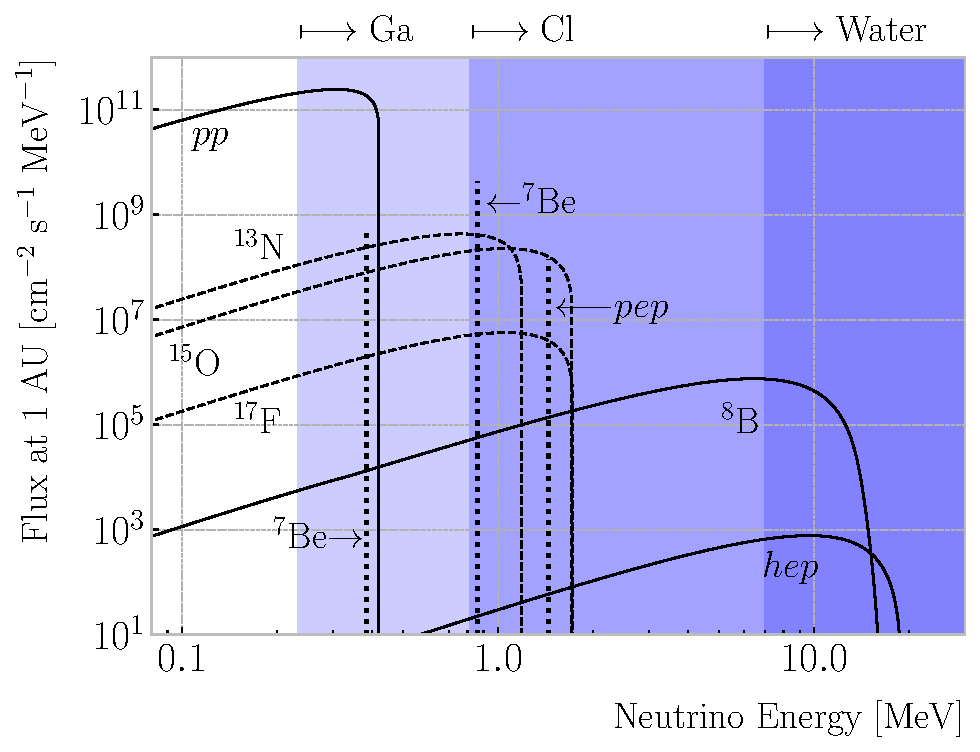
\includegraphics[width=.75\linewidth]{Images/Nu/solar_neutrino_flux.pdf}
	\caption[Solar neutrino fluxes for the solar model BS05(OP).]{Solar neutrino fluxes for the solar model BS05(OP). The detection thresholds for Gallium, Chlorine and water-based experiments are also shown. Figure adapted from Ref. \cite{Bahcall2004}.}
	\label{fig:solar_nu_flux}
\end{figure}

The results of the experiment were compared to the theoretical predictions made by J. Bahcall \cite{Bahcall1968}. During its operation from 1968 to 2002, the experiment observed a solar $\nu_{e}$ flux that was approximately a third of the total prediction \cite{Cleveland1998}.

In the early 1990s, the SAGE \cite{SAGE2009} and GALLEX \cite{GALLEX2010} experiments started operations. The detection principle used for both experiments was similar to that of the Homestake experiment, but using $\prescript{71}{}{\mathrm{Ga}}$ instead of $\mathrm{C}_{2}\mathrm{Cl}_{4}$. With a detection threshold of $0.233~\mathrm{MeV}$, the Gallium-based experiments were able to observe the $pp$ neutrino flux. Both experiments measured a solar electron neutrino flux that was a factor of two lower than the predictions, demonstrating that this deficit was energy-dependent.

In the early 2000s, the SNO experiment put an end to the solar neutrino puzzle \cite{Ahmad2001,Ahmad2002}. Thanks to its directionality capabilities, being a Cherenkov light detector, as well as to its heavy water target, SNO measured the total solar neutrino flux through the NC process:
\begin{equation}
	\nu_{\alpha} + d \longrightarrow n + p + \nu_{\alpha},
\end{equation}
where $\alpha = e, \mu, \tau$. This measurement agreed with the solar model predictions. Then, measuring the CC reaction:
\begin{equation}
	\nu_{e} + d \longrightarrow p + p + e^{-},
\end{equation}
they were able to establish that the $\nu_{\mu}$ and $\nu_{\tau}$ solar fluxes are in fact non-zero, revealing that electron neutrinos were transitioning into different flavours.

\subsection{The atmospheric neutrino problem}

When cosmic-rays interact with the atoms in the upper atmosphere, a plethora of hadrons, mainly $\pi$ and $K$ mesons, are produced. In particular, for the charged pions, we have the following decay chain dominates:
\begin{equation}
	\begin{split}
		&\pi^{+} \longrightarrow \mu^{+} + \nu_{\mu},\\
		&\mu^{+} \longrightarrow e^{+} + \bar{\nu}_{\mu} + \nu_{e},
	\end{split}
\end{equation}
and similar for the antiparticles. For neutrino energies $< 1~\mathrm{GeV}$, the ratio:
\begin{equation}
	\frac{N(\nu_{\mu}+\bar{\nu}_{\mu})}{N(\nu_{e}+\bar{\nu}_{e})},
\end{equation}
of produced neutrinos and antineutrinos is, in good approximation, equal to two \cite{Gaisser2002}.

During the 1980s, several proton decay experiments, like Kamiokande \cite{Hirata1988}, IMB \cite{Casper1991}, MACRO \cite{Ambrosio1998}, and Soudan-2 \cite{Allison1997}, measured the flux of atmospheric neutrinos. This was an important part of their research programme, as the atmospheric neutrinos constitute their main background. All these experiments reported an atmospheric neutrino ratio lower than the predictions.

\begin{figure}[t]
	\centering
	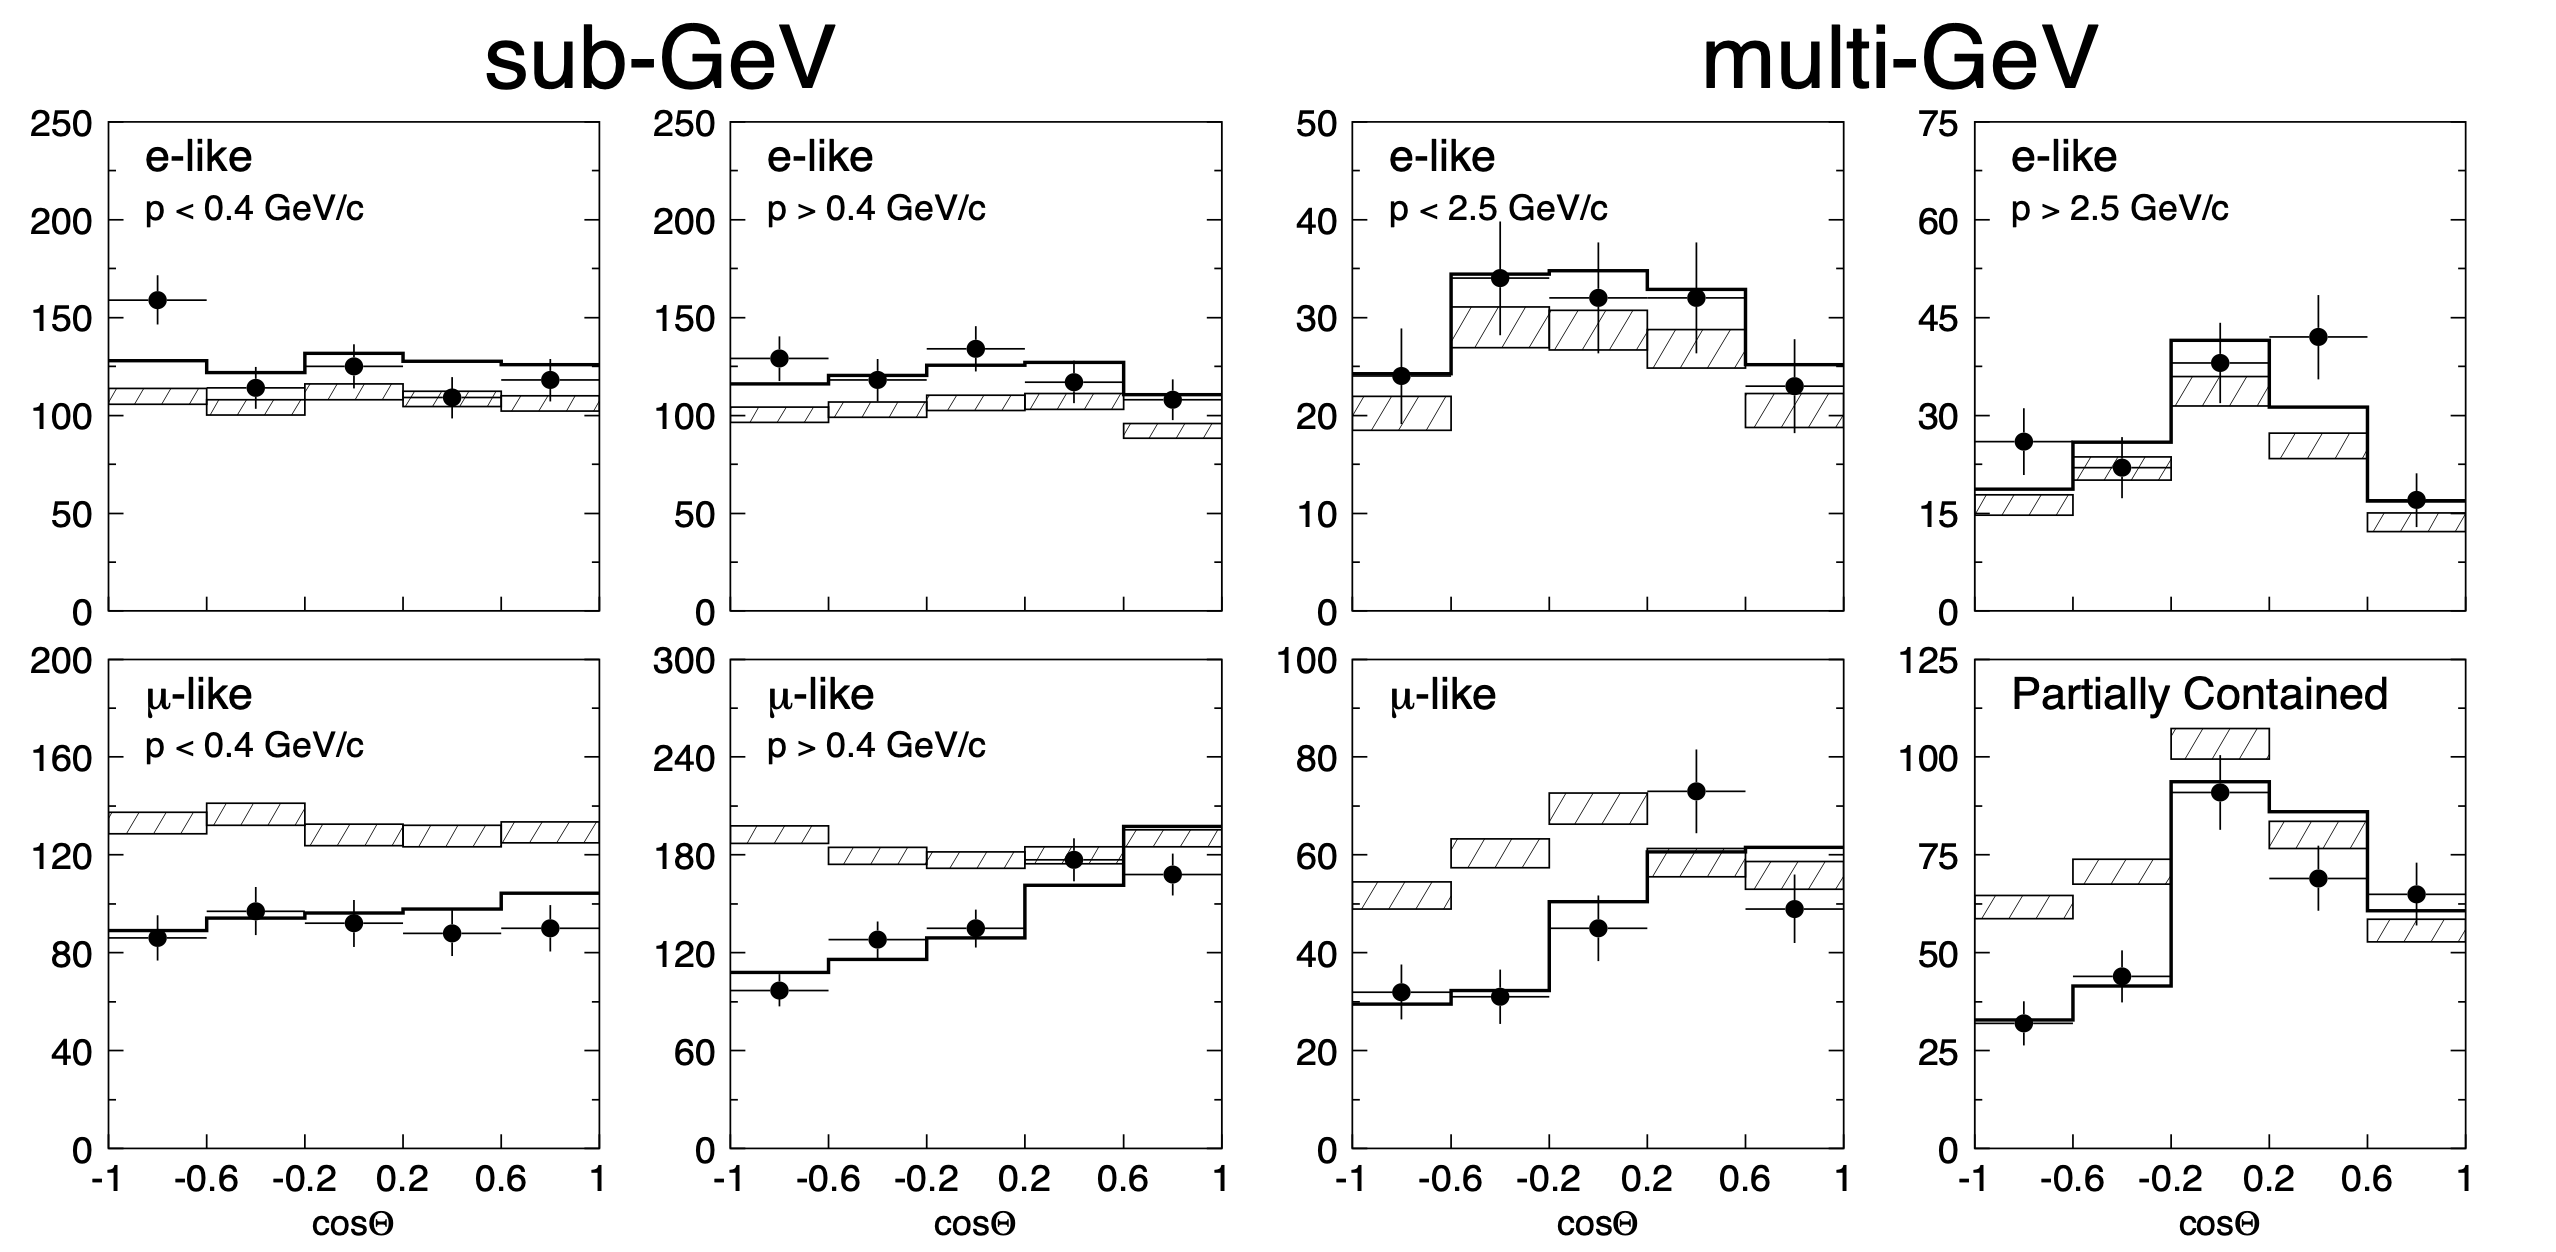
\includegraphics[width=.90\linewidth]{Images/Nu/superk_oscillations.png}
	\caption[Zenith angle distributions for the selected $\nu_{e}$ and $\nu_{\mu}$ events in the SK detector.]{Zenith angle distributions for the selected $\nu_{e}$ (top row) and $\nu_{\mu}$ (bottom row) events in the SK detector. The hatched region corresponds to the expectation in the case of no oscillations, whereas the solid line indicates the best-fit in the case of $\nu_{\mu} \rightarrow \nu_{\tau}$ oscillations. Figure taken from Ref. \cite{SuperKamiokande1998}.}
	\label{fig:atmospheric_nu_osc}
\end{figure}

A few years before the SNO discovery, in 1998, Super-Kamiokande (SK) collaboration measured the atmospheric $\nu_{e}$ and $\nu_{\mu}$ spectra as a function of the zenith angle \cite{SuperKamiokande1998}. Upward-going particles have negative zenith angle, $\mathrm{cos}~\Theta < 0$, indicating that they entered from the bottom of the detector. These upward-going neutrinos had to travel through the Earth in order to reach the detector, allowing SK to probe a broad range of baselines. Figure \ref{fig:atmospheric_nu_osc} shows the reported distributions (black dots), compared to the no oscillations prediction (hatched region). This measurement confirmed that muon neutrinos transition to other flavours, and that this phenomenon depends both on the energy and the path length of the neutrino.

The SK and SNO findings provided definitive evidence for the existence of neutrino oscillations, and therefore non-zero neutrino masses. This constitutes one of the groundbreaking discoveries of modern physics and has acted as driving force for beyond the Standard Model (BSM) physics. The minimal extension of the SM we can do to address these phenomena is introducing different masses for at least two of the neutrinos. This way, we are left with three neutrino mass eigenstates $\nu_{1}$, $\nu_{2}$, and $\nu_{3}$, with masses $m_{1}$, $m_{2}$, and $m_{3}$ respectively, which in general will not coincide with the flavour eigenstates, $\nu_{e}$, $\nu_{\mu}$, and $\nu_{\tau}$.

\section{Massive neutrinos}\label{sec:nu_mass}

The existence of neutrino oscillations imply that neutrinos are massive particles. However, as we have seen before, within the SM neutrinos are massless, as they do not have a mass term in the Lagrangian. If one wants to give neutrinos a mass, the particle content of the SM needs to be expanded.

A way of generating massive neutrinos while maintaining gauge invariance is by introducing an arbitrary number of sterile neutrinos $N_{i}$, $i=1,\dots,m$. These allow for two different types of neutrino mass terms:
\begin{equation}\label{2.10}
	-\mathcal{L}_{M_{\nu}} = \sum_{i=1}^{m} \sum_{j=1}^{3} M^{ij}_{D} \bar{N}_{i} \nu_{Lj} + \frac{1}{2} \sum_{i=1}^{m} \sum_{j=1}^{m} M^{ij}_{N} \bar{N}_{i} N^{c}_{j} + \mathrm{h.c.},
\end{equation}
where $M_{D}$ is a complex $m \times 3$ matrix and $M_{N}$ a complex and symmetric $m \times m$ matrix. The first term, often referred to as the Dirac mass term, arises from the corresponding Yukawa interaction after the spontaneous electroweak symmetry breaking, similar to the other fermions. The second term, called the Majorana mass term, is allowed in the Lagrangian, as it is a singlet of the gauge group. However, it violates lepton number conservation by two units.

If one imposes lepton number symmetry conservation, the Majorana term must banish, $M_{N}=0$. In this case, if $m=3$ we can identify the sterile neutrinos as the right-handed component of the neutrino field. The Dirac mass matrix can be diagonalised using two unitary matrices, $V^{\nu}_{R}$ and $V^{\nu}_{L}$, as:
\begin{equation}
	M_{D} = V^{\nu}_{R}~\mathrm{diag}(m_{1}, m_{2}, m_{3})~V^{\nu \dagger}_{L},
\end{equation}
where $m_{i}$, $i=1,2,3$ are the masses of the three neutrino mass eigenstates.

The neutrino mass term can be written in term of the resulting eigenstates as:
\begin{equation}
	-\mathcal{L}_{M_{\nu}} = \sum_{i=1}^{3} m_{i}~\bar{\nu}_{Di} \nu_{Di},
\end{equation}
with:
\begin{equation}
	\nu_{Di} = \left(V^{\nu \dagger}_{L}~\nu_{L}\right)_{i} + \left(V^{\nu \dagger}_{R}~N\right)_{i}.
\end{equation}

In this scenario, both the low energy particle budget and the symmetries of the SM have to be modified. Moreover, the masses of the neutrinos are generated exclusively through the Higgs mechanism, which does not explain why they are much smaller than those of the charged leptons.

Going back to the general case, we can re-write Eq. (\ref{2.10}) in matrix form as:
\begin{equation}
	-\mathcal{L}_{M_{\nu}} = \frac{1}{2} \begin{pmatrix}\bar{\nu}^{c}_{L},&\bar{N}\end{pmatrix} \begin{pmatrix}0 & M_{D}^{T}\\M_{D} & M_{N}\end{pmatrix}\begin{pmatrix}\nu_{L}\\N^{c}\end{pmatrix} + \mathrm{h.c.} = \bar{\nu}^{c} M_{\nu} \nu + \mathrm{h.c.},
\end{equation}
with $\nu=\begin{pmatrix}\nu_{L}, & N^{c}\end{pmatrix}^{T}$ being a $(3+m)$-dimensional vector grouping the active and the sterile neutrinos. The matrix $M_{\nu}$, which is a complex $(3+m)\times(3+m)$ symmetric matrix, can be diagonalised by means of a unitary matrix $V^{\nu}$, yielding:
\begin{equation}
	M_{\nu} = V^{\nu}~\mathrm{diag}(m_{1}, m_{2}, \dots, m_{3+m})~V^{\nu T}.
\end{equation}

Using this eigendecomposition, the neutrino mass term can be expressed as:
\begin{comment}
\begin{equation}
	\begin{split}
		-\mathcal{L}_{M_{\nu}} &= \frac{1}{2} \sum_{i=1}^{3+m} m_{i} \left[\left(\vphantom{V^{\nu \dagger}}\bar{\nu}^{c}~V^{\nu}\right)_{i} \left(V^{\nu \dagger}~\nu\right)_{i} + \left(\vphantom{V^{\nu \dagger}}\bar{\nu}~V^{\nu}\right)_{i} \left(V^{\nu \dagger}~\nu^{c}\right)_{i}\right]\\
		&= \frac{1}{2} \sum_{i=1}^{3+m} m_{i}~\bar{\nu}_{M i} \nu_{M i},
	\end{split}
\end{equation}
\end{comment}
\begin{equation}
	-\mathcal{L}_{M_{\nu}} = \frac{1}{2} \sum_{i=1}^{3+m} m_{i}~\bar{\nu}_{M i} \nu_{M i},
\end{equation}
where the states $\nu_{M i}$, commonly referred to as Majorana neutrinos, are defined as:
\begin{equation}
	\nu_{M i} = \left(V^{\nu\dagger}~\nu\right)_{i} + \left(V^{\nu\dagger}~\nu\right)^{c}_{i},
\end{equation}
in such a way that the Majorana condition, $\nu^{c}_{M} = \nu_{M}$, holds true.

As a consequence of the Majorana condition, the neutrino and the antineutrino states can be described in terms of a single field. As opposed to the charged leptons, which need to be represented by a four-component or Dirac spinor, the Majorana neutrino is described by a two-component or Weyl spinor.

If the eigenvalues of the Majorana mass matrix, $M_{N}$, are much larger than the electroweak symmetry breaking scale, the diagonalisation of $M_{\nu}$ leads to $3$ light and $m$ heavy neutrino states:
\begin{equation}
	-\mathcal{L}_{M_{\nu}} = \frac{1}{2} \bar{\nu}_{l} M_{l} \nu_{l} + \frac{1}{2} \bar{\nu}_{h} M_{h} \nu_{h},
\end{equation}
where the two mass matrices are given by:
\begin{equation}
	\begin{split}
		M_{l} &\simeq -V_{l}^{T} M_{D}^{T} M_{N}^{-1} M_{D} V_{l},\\
		M_{h} &\simeq V_{h}^{T} M_{N} V_{h},
	\end{split}
\end{equation}
with $V_{l}$ and $V_{h}$ two unitary matrices.

This scenario represents the so-called see-saw mechanism \cite{Minkowski1977,Gell-Mann1979,Yanagida1979,Mohapatra1979,Schechter1980}. The name comes from the fact that the masses of the heavy states are proportional to $M_{N}$, whereas for the light states they are proportional to $M_{N}^{-1}$. While both the heavy and the light neutrinos are Majorana particles, it can be shown that the heavy states are mainly right-handed, whereas the light ones are mostly left-handed.

\section{Neutrino oscillation formalism}\label{sec:nu_oscillations}

Neutrino oscillations were first proposed in 1958 by B. Pontecorvo \cite{Pontecorvo1957a}, inspired by the neutral kaon oscillation phenomenon \cite{Gell-Mann1955}. Neutral kaons, $K^{0}$ and $\bar{K}^{0}$, have opposite strangeness ($\pm 1$) and are produced in strong processes. It was observed that, when having a beam initially pure of neutral kaons of one type, these would transition into their antiparticles while propagating. Because the weak interaction does not conserve strangeness, neutral kaons can change their identity via the processes shown in Fig. \ref{fig:kaon_oscillations}.

The mixing considered initially by Pontecorvo was between the neutrino and the antineutrino states, as only one neutrino flavour was known at the time. After the discovery of the muon neutrino, the mixing between flavours was also explored \cite{Pontecorvo1967}.

In the general case, we have $3$ active and $m$ sterile neutrinos, resulting in $3+m$ neutrino mass eigenstates. Working in the mass basis, the leptonic charged-current Lagrangian can be written as:
\begin{equation}
	-\mathcal{L}_{\mathrm{CC}}^{lep} = \frac{g}{\sqrt{2}} \begin{pmatrix}\bar{e}_{L},~ \bar{\mu}_{L},~ \bar{\tau}_{L}\end{pmatrix} \gamma^{\mu} U \begin{pmatrix}\nu_{1}\\\nu_{2}\\\vdots\\\nu_{3+m}\end{pmatrix} W_{\mu}^{+} + \mathrm{h.c.},
\end{equation}
where $U$ is a $3\times(3+m)$ matrix which obeys $UU^{\dagger} = I_{3 \times 3}$, but in general will not be unitary, $U^{\dagger}U\neq I_{(3+m) \times (3+m)}$.

The leptonic mixing matrix, $U$, establishes how the neutrino mass states couple to the charged leptons. In general, a complex $n \times n$ matrix can be fully specified by $2n^{2}$ real parameters. If the matrix is unitary, then the number of independent parameters reduces to $n^{2}$, as one has to impose $n$ normalisation and $n(n-1)$ orthogonality constraints. In our case, we can further reduce the number of parameters by performing a phase redefinition of the charged lepton fields, without affecting the physics. This is not true for the neutrinos. As they may be their own antiparticles, one is not allowed to remove any physically relevant phases. If we consider $n$ generations of leptons, the total number of parameters in the mixing matrix is $n^{2}-n$. Out of these, half of them are mixing angles, while the other half are complex phase factors.

\begin{figure}[t]
	\begin{subfigure}{0.5\textwidth}
		\centering
		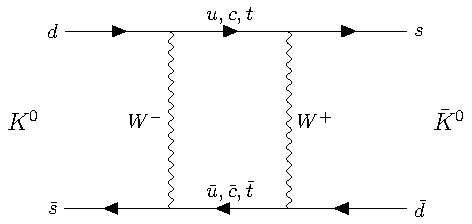
\includegraphics[width=.90\linewidth]{Images/Nu/feynman_kaon_1.pdf}
	\end{subfigure}
	\begin{subfigure}{0.5\textwidth}
		\centering
		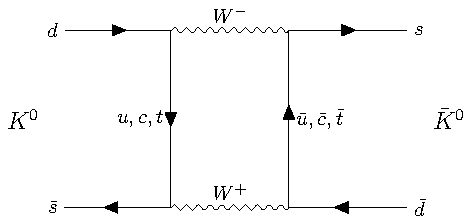
\includegraphics[width=.90\linewidth]{Images//Nu/feynman_kaon_2.pdf}
	\end{subfigure}
	\caption{$K^{0} \leftrightharpoons \bar{K}^{0}$ mixing through $W^{\pm}$ exchange.}
	\label{fig:kaon_oscillations}
\end{figure}

Considering the extended SM without any additional sterile neutrino states, the  resulting $3 \times 3$ mixing matrix is unitary. This matrix, often called the Pontecorvo-Maki-Nakagawa-Sakata (PMNS) matrix \cite{Pontecorvo1957, Maki1962}, relates the set of active neutrinos and the three mass eigenstates as:
\begin{equation}\label{2.1}
\ket{\nu_{\alpha}} = \sum_{i=1}^{3} U^{*}_{\alpha i} \ket{\nu_{i}},
\end{equation}
where the Greek index $\alpha$ denotes the flavour $\{e,\mu,\tau\}$ and the Latin index $i$ the mass state $\{1,2,3\}$. This leptonic mixing matrix may be parametrized in terms of 6 parameters, 3 of which are mixing angles $\theta_{12}$, $\theta_{13}$ and $\theta_{23}$, one CP-violating phase $\delta_{CP}$ and 2 Majorana phases $\alpha$ and $\beta$:
\begin{equation}\label{2.2}
	U = \begin{pmatrix}1&0&0\\0&c_{23}&s_{23}\\0&-s_{23}&c_{23}\end{pmatrix} \begin{pmatrix}c_{13}&0&s_{13} \mathrm{e}^{-i\delta_{CP}}\\0&1&0\\-s_{13} \mathrm{e}^{i\delta_{CP}}&0&c_{13}\end{pmatrix} \begin{pmatrix}c_{12}&s_{12}&0\\-s_{12}&c_{12}&0\\0&0&1\end{pmatrix} \begin{pmatrix}1&0&0\\0&\mathrm{e}^{i\alpha}&0\\0&0&\mathrm{e}^{i\beta}\end{pmatrix},
\end{equation}
where $c_{ij} \equiv \cos \theta_{ij}$ and $s_{ij} \equiv \sin \theta_{ij}$. This matrix is analogous to the Cabibbo-Kobayashi-Maskawa (CKM) matrix in the quark sector. If neutrinos are Dirac fermions, we can drop the Majorana phases in the PMNS matrix, as in this case we can perform the phase redefinitions. However, these phases play no role on the neutrino oscillation phenomenology.

In the case that additional sterile neutrinos states are present, the full leptonic mixing matrix would not be unitary in general. For instance, in the see-saw scenario, the $3 \times 3$ submatrix for the three light Majorana neutrinos is not unitary. However, the deviations from unitarity are of the order $\mathcal{O}(M_{D}/M_{N})$, and therefore expected to be negligible.

\subsection{Oscillations in vacuum}

Consider the case where a neutrino of flavour $\alpha$ is produced at $t=0$, and then it propagates through vacuum. Such a state will evolve in time according to the relation:
\begin{equation}
\ket{\nu_{\alpha}(\vec{x}, t)} = \sum_{i=1}^{3} U^{*}_{\alpha i} \mathrm{e}^{-i(E_{i}t-\vec{p}_{i}\cdot\vec{x})} \ket{\nu_{i}(\vec{x}=\vec{0},t=0)},
\end{equation}
in the plane wave approximation, as the mass eigenstates are also eigenstates of the free Hamiltonian.
\begin{comment}
Now, if we express the mass eigenstates as a superposition of flavour eigenstates, the last expression can be rewritten as:
\begin{equation}\label{2.4}
\ket{\nu_{\alpha}(t)} = \sum_{\beta} \sum_{i=1}^{3} U_{\beta i} \mathrm{e}^{-iE_{i}t} U^{*}_{\alpha i} \ket{\nu_{\beta}}.
\end{equation}
\end{comment}

This way, the probability for the neutrino to transition from flavour $\alpha$ to flavour $\beta$ will be given by:
\begin{equation}
\begin{split}
	P(\nu_{\alpha} \rightarrow \nu_{\beta}) = \left|\braket{\nu_{\beta}}{\nu_{\alpha}(\vec{x}, t)}\right|^{2} &= \left|\sum_{i=1}^{3} \sum_{j=1}^{3} U^{*}_{\alpha i} U_{\beta j} \mathrm{e}^{-i(E_{i}t-\vec{p}_{i}\cdot\vec{x})} \braket{\nu_{j}}{\nu_{i}}\right|^{2}\\
	&= \left|\sum_{i=1}^{3} U^{*}_{\alpha i} U_{\beta i} \mathrm{e}^{-i(E_{i}t-\vec{p}_{i}\cdot\vec{x})}\right|^{2},
\end{split}
\end{equation}
where we have used the orthogonality relation $\braket{\nu_{i}}{\nu_{j}} = \delta_{ij}$. A usual approximation to take at this point is to consider ultra-relativistic neutrinos, i.e. $p_{i} \simeq E$, so we can write the dispersion relations as:
\begin{equation}
E_{i} = \sqrt{p_{i}^{2} + m_{i}^{2}} \approx E + \frac{m_{i}^{2}}{2 E}.
\end{equation}

In the end, assuming $t \approx L$ where $L$ is the distance between the production and the detection points, the probability for the $\nu_{\alpha} \rightarrow \nu_{\beta}$ transition becomes:
\begin{equation}
\begin{split}
P(\nu_{\alpha} \rightarrow \nu_{\beta}) &= \sum_{i,j} U^{*}_{\alpha i} U_{\beta i} U_{\alpha j} U^{*}_{\beta j} \mathrm{e}^{-i\frac{\Delta m^{2}_{ij}}{2E}L}\\
&=\delta_{\alpha\beta} - 4 \sum_{i<j} \mathfrak{Re}\left[U^{*}_{\alpha i} U_{\beta i} U_{\alpha j} U^{*}_{\beta j}\right] \sin^{2}\left(\frac{\Delta m^{2}_{ij}}{4E}L\right)\\
&\phantom{=}+ 2  \sum_{i<j} \mathfrak{Im}\left[U^{*}_{\alpha i} U_{\beta i} U_{\alpha j} U^{*}_{\beta j}\right] \sin\left(\frac{\Delta m^{2}_{ij}}{2E}L\right),
\end{split}
\end{equation}
where $\Delta m^{2}_{ij}$ is the difference of the squared masses of the $j$th and $i$th neutrino mass eigenvalues. At this point, it is usual to write the phase responsible for the oscillations as:
\begin{equation}\label{2.8}
\Delta_{ij} \equiv \frac{\Delta m^{2}_{ij}}{4E}L \simeq 1.27 \frac{\Delta m^{2}_{ij}}{(\mathrm{eV}^{2})} \frac{L}{(\mathrm{km})} \frac{(\mathrm{GeV})}{E}.
\end{equation}

Notice that, in the case of antineutrinos, the only difference would be the sign of the last term in the oscillation probability. As the process $\bar{\nu}_{\alpha} \rightarrow \bar{\nu}_{\beta}$ is the CP-mirror image of $\nu_{\alpha} \rightarrow \nu_{\beta}$, the differences between their oscillation probabilities would be a measure of CP symmetry violation:
\begin{equation}\label{2.9}
\begin{split}
A^{\alpha\beta}_{CP}&=P(\nu_{\alpha} \rightarrow \nu_{\beta})-P(\bar{\nu}_{\alpha} \rightarrow \bar{\nu}_{\beta})\\
&=4  \sum_{i<j} \mathfrak{Im}\left[U^{*}_{\alpha i} U_{\beta i} U_{\alpha j} U^{*}_{\beta j}\right] \sin 2\Delta_{ij}.
\end{split}
\end{equation}

Assuming that CPT invariance holds, then the following relation must be true:
\begin{equation}
	P(\nu_{\alpha} \rightarrow \nu_{\beta}) = P(\bar{\nu}_{\beta} \rightarrow \bar{\nu}_{\alpha}),
\end{equation}
as these two process are related by the CPT symmetry. From the definition of probability, we also must have:
\begin{equation}
	\sum_{\beta} P(\nu_{\alpha} \rightarrow \nu_{\beta}) = \sum_{\beta} P(\bar{\nu}_{\alpha} \rightarrow \bar{\nu}_{\beta}) = 1,
\end{equation}
where the sum includes all flavours, including $\alpha$. From these two constraints, one can probe that:
\begin{equation}
	A^{\alpha\beta}_{CP} = - A^{\beta\alpha}_{CP},
\end{equation}
and in particular:
\begin{equation}
	A^{\alpha\alpha}_{CP} = 0.
\end{equation}

A direct consequence of this last relation is that there are no observable CP-violating effects in the so-called disappearance experiments. One needs to perform appearance experiments, where the flavour detected is different from the original flavour, in order to measure the CP asymmetry. Neutrino experiments often report the amount of CP-violation through the Jarlskog invariant. In terms of the parametrisation typically used to write the PMNS matrix, it is given by:
\begin{equation}
	J = \frac{1}{8} \mathrm{cos}~\theta_{13}~\mathrm{sin}~2\theta_{12}~\mathrm{sin}~2\theta_{13}~\mathrm{sin}~2\theta_{23}~\mathrm{sin}~\delta_{CP}.
\end{equation}
The Jarlskog invariant can be used to compare the amount of CP-violation in the lepton and the quark sectors, where $J=3.12^{+0.13}_{-0.12} \times 10^{-5}$ in the latter \cite{ParticleDataGroup2024}.

\subsection{Oscillations in matter}

When neutrinos propagate through matter, their oscillation can be affected in mainly two ways. First, neutrinos can inelastically scatter with nuclei, thus destroying the coherent propagation of their quantum state. Nevertheless, in most cases this effect is negligible (even in very dense mediums like the core of the Sun). Second, neutrinos can also experience coherent or forward scatterings, that can affect their oscillation but not lose the coherent propagation of the state.

The first proposed model to account for neutrino oscillations in matter was proposed by Mikhaev, Smirnov and Wolfenstein (MSW) \cite{Wolfenstein1977}. It relies on the fact that, as the only charged lepton present in ordinary matter is the electron, electron neutrinos can undergo both charged and neutral-current interactions with matter whereas for muon and tau neutrinos just neutral currents are possible.

An illustrative way to introduce the MSW mechanism is by considering the two flavours case. It can be shown that the evolution of the two flavour eigenstates in vacuum is given by the following time-dependent Schrödinger equation:
\begin{equation}
	i \frac{\mathrm{d}}{\mathrm{d}t} \begin{pmatrix}\nu_{e}\\\nu_{\mu}\end{pmatrix} = H_{V} \begin{pmatrix}\nu_{e}\\\nu_{\mu}\end{pmatrix},
\end{equation}
with a vacuum Hamiltonian given by:
\begin{comment}
\begin{equation}
	H_{V} = \frac{m_{1}^{2}+m_{2}^{2}}{4E} \begin{pmatrix}1&0\\0&1\end{pmatrix}+\frac{\Delta m^{2}}{4E} \begin{pmatrix}-\mathrm{cos}~2\theta&\mathrm{sin}~2\theta\\\mathrm{sin}~2\theta&\mathrm{cos}~2\theta\end{pmatrix},
\end{equation}
\end{comment}
\begin{equation}
	H_{V} = \frac{\Delta m^{2}}{4E} \begin{pmatrix}-\mathrm{cos}~2\theta&\mathrm{sin}~2\theta\\\mathrm{sin}~2\theta&\mathrm{cos}~2\theta\end{pmatrix},
\end{equation}
where $\Delta m^{2}$ is the mass splitting between the two neutrino states and $\theta$ the only mixing angle. For simplicity, I omit the terms of the Hamiltonian that are proportional to the identity, as they do not affect the oscillation phenomenology.

The NC contribution to the matter potential is identical for all the flavours, and has the form:
\begin{equation}
	V_{\mathrm{NC}} = -\frac{G_{F}}{\sqrt{2}} N_{n}(x),
\end{equation}
where $G_{F}$ is the Fermi constant and $N_{n}(x)$ the local neutron density. Because it is common to all flavours, I do not take it into account in the effective Hamiltonian, as it would appear as a term proportional to the identity. The CC component only affects the electron neutrino (and antineutrino). It can be written as:
\begin{equation}
	V_{\mathrm{CC}} = \pm \sqrt{2} G_{F} N_{e}(x),
\end{equation}
with $N_{e}(x)$ being the local electron density in the material. In the end, the effective Hamiltonian which describes the propagation of the flavour eigenstates in matter only contains an extra $\nu_{e}-\nu_{e}$ element:
\begin{equation}
	H_{M} = H_{V} + \begin{pmatrix}V_{\mathrm{CC}}&0\\0&0\end{pmatrix}.
\end{equation}

The solution to the Schrödinger equation greatly simplifies if one considers the case of a constant matter density. In that case, the effective Hamiltonian can be diagonalised, obtaining the effective neutrino mass eigenstates in matter. It can be re-written in the same form as the vacuum Hamiltonian:
\begin{equation}
	H_{M} = \frac{\Delta m_{m}^{2}}{4E} \begin{pmatrix}-\mathrm{cos}~2\theta_{m}&\mathrm{sin}~2\theta_{m}\\\mathrm{sin}~2\theta_{m}&\mathrm{cos}~2\theta_{m}\end{pmatrix},
\end{equation}
where the effective mass splitting and the effective mixing angle are given by:
\begin{equation}
	\begin{split}
		\Delta m_{m}^{2} = \lambda \Delta m_{m}^{2},\\
		\mathrm{sin}~2\theta_{m} = \frac{\mathrm{sin}~2\theta_{m}}{\lambda}
	\end{split}
\end{equation}
with:
\begin{equation}
	\begin{split}
		\lambda &= \sqrt{(\mathrm{cos}~2\theta - A)^{2} + \mathrm{sin}^{2}~2\theta},\\
		A &= \pm \frac{2\sqrt{2}G_{F}N_{e}E}{\Delta m^{2}}.
	\end{split}
\end{equation}

In terms of the effective matter oscillation parameters, the transition probability $\nu_{e} \rightarrow \nu_{\mu}$ (in the two flavour approximation) reads:
\begin{equation}
	P(\nu_{e} \rightarrow \nu_{\mu}) = \mathrm{sin}^{2}~2\theta_{m} ~ \mathrm{sin}^{2}\left(\frac{\Delta m_{m}^{2}}{2E}L\right)
\end{equation}
From this last equation one can see that, when $\mathrm{cos}~2\theta = A > 0$ the oscillations are greatly enhanced. This effect is known as the MSW resonance. For the neutrinos, this resonant condition is only satisfied if $\Delta m^{2}>0$ (the opposite is true for antineutrinos). This is can be exploited by long baseline experiments, which can gain sensitivity to the neutrino mass hierarchy through matter effects.

\subsection{Current status of neutrino oscillations}

A wide range of neutrino experiments provide experimental input to the neutrino oscillation framework, both using natural or synthetic neutrino sources. The results from one of the neutrino global fit analyses, shown in Tab. \ref{tab:neutrino_global_fit} \footnote{These are the results reported during M. T\'{o}rtola's talk at Neutrino 2024 (see this \href{https://agenda.infn.it/event/37867/contributions/233956/attachments/121839/178002/MTortola-Neutrino2024.pdf}{link}). I need to keep an eye and see if they publish these or other updated results in the near future.}, summarise well our current understanding of the different oscillation parameters.

\textbf{Solar neutrino experiments} detect neutrinos produced in thermonuclear reactions inside the Sun, mainly from the so-called $pp$ chain and the CNO cycle. These neutrinos have a typical energy in the range from $0.1$ to $20 \ \mathrm{MeV}$. These experiments (Homestake \cite{Homestake1998}, GALLEX \cite{GALLEX2010}, SAGE \cite{SAGE2009}, Borexino \cite{Borexino2011}, Super-Kamiokande \cite{Super-Kamiokande2005} and SNO \cite{SNO2011}) provide the best sensitivities to $\theta_{12}$ and $\Delta m^{2}_{21}$.

\textbf{Atmospheric neutrino experiments} detect the neutrino flux produced when cosmic rays scatter with particles in Earth's atmosphere. These collisions generate particle showers that eventually produce electron and muon neutrinos (and antineutrinos). Their energies range from few $\mathrm{MeV}$ to about $10^{9} \ \mathrm{GeV}$. Experiments, like Super-Kamiokande \cite{Super-Kamiokande2017} and IceCube \cite{IceCube2017} use atmospheric neutrinos to measure oscillations and are specially sensitive to $\theta_{23}$ and $\Delta m^{2}_{32}$.

\textbf{Reactor neutrino experiments} look for the $\bar{\nu}_{e}$ spectrum produced by nuclear reactors, with energies in the $\mathrm{MeV}$ scale. Depending on the distance to the source, long-baseline experiments like KamLAND \cite{KamLAND2013} are sensitive to the solar mass splitting $\Delta m^{2}_{21}$ whereas much shorter baseline experiment such as RENO \cite{RENO2018} or DayaBay \cite{DayaBay2018} measure $\theta_{13}$ and $\Delta m^{2}_{31}$.

\textbf{Accelerator experiments} measure neutrino fluxes generated in particle accelerators. Usually mesons are produced in the accelerator to be focused into a beam, then some decay to muon neutrinos and the rest are absorbed by a target. Depending on the configuration one can obtain a beam made of mostly neutrinos or antineutrinos. The typical energies of these neutrinos are in the $\mathrm{GeV}$ range. Experiments such as NOvA \cite{Nova2020}, T2K \cite{T2K2020}, MINOS \cite{MINOS2014}, OPERA \cite{OPERA2018} and K2K \cite{K2K2006} (and in the future DUNE \cite{DUNE2020}) are primarily sensitive to $\theta_{13}$, $\theta_{23}$ and $\Delta m^{2}_{32}$. Also, in the coming years  DUNE \cite{DUNE2020} and Hyper-Kamiokande \cite{Hyper-Kamiokande2019} will be sensitive to $\delta_{CP}$.

\begin{table}
\centering
\caption[Summary of neutrino oscillation parameters determined in the Neutrino Global Fit of 2020.]{Summary of neutrino oscillation parameters determined in the Neutrino Global Fit of 2020 \cite{deSalas2020}.}
	\begin{tabular}{c|c|c}
		Parameter                                               & Best fit $\pm ~ 1\sigma$ & $3 \sigma$ range   \\[1mm] \hline \rule{0pt}{1.1\normalbaselineskip}
		$\Delta m^{2}_{21}~[\mathrm{eV}^{2} \times 10^{-5}]$                   & $7.55^{+0.22}_{-0.20}$ & $6.98-8.19$\\[3mm]
		$\left|\Delta m^{2}_{31}\right|~[\mathrm{eV}^{2}\times 10^{-3}]$ (NO) & $2.51^{+0.02}_{-0.03}$    & $2.43-2.58$\\[2mm]
		$\left|\Delta m^{2}_{31}\right|~[\mathrm{eV}^{2}\times 10^{-3}]$ (IO) & $2.41^{+0.03}_{-0.02}$ & $2.34-2.49$    \\[3mm]
		$\sin^{2} \theta_{12} / 10^{-1}$ & $3.04 \pm 0.16$ & $2.57-3.55$ \\[3mm]
		$\sin^{2} \theta_{23} / 10^{-1}$ (NO) & $5.64^{+0.15}_{-0.21}$ & $4.23-6.04$ \\[2mm]
		$\sin^{2} \theta_{23} / 10^{-1}$ (IO) & $5.64^{+0.15}_{-0.18}$ & $4.27-6.03$ \\[3mm]
		$\sin^{2} \theta_{13} / 10^{-2}$ (NO) & $2.20^{+0.05}_{-0.06}$ & $2.03-2.38$ \\[2mm]
		$\sin^{2} \theta_{13} / 10^{-2}$ (IO) & $2.20^{+0.07}_{-0.04}$ & $2.04-2.38$ \\[3mm]
		$\delta_{CP} / \pi$ (NO) & $1.12^{+0.16}_{-0.12}$ & $0.76-2.00$ \\[2mm]
		$\delta_{CP} / \pi$ (IO) & $1.50^{+0.13}_{-0.14}$ & $1.11-1.87$
	\end{tabular}
	\label{tab:neutrino_global_fit}
\end{table}

\section{Open questions in the neutrino sector}\label{sec:nu_open_questions}

A crucial question that remains open these days, and is of vital importance for oscillation phenomena, is whether the mass eigenvalue $\nu_{3}$ is the heaviest (what we call normal ordering) or the lightest (referred to as inverted ordering) of the mass eigenstates. In other words, this means that we do not know the sign of $\Delta m^{2}_{32}$, so we can either have $m_{1}<m_{2}<m_{3}$ (NO) or $m_{3}<m_{1}<m_{2}$ (IO).

Another big puzzle is related to the value of $\delta_{CP}$. Nowadays it is poorly constrained, with all values between $\pi$ and $2\pi$ being consistent with data. A prospective measurement different from $\delta_{CP}=0,\pi$ will predict CP-violation in the leptonic sector, and thus contribute along with the one measured in the quark sector to the total amount of CP-violation. Although it is true that these two contributions by themselves are not enough to explain the matter anti-matter asymmetry in our universe, the amount of CP-violation in the leptonic sector can be key to explain such imbalance.

Both of these questions, because of their nature, could be understood thanks to future oscillation experiments.

Notwithstanding, there are other mysteries that can not be unveiled just by conducting oscillation experiments, as certain quantities do not influence these phenomena. Among these there is the question of the absolute values of the neutrino masses. Depending on the value of the lightest of the neutrino masses we can have different mass spectra, from hierarchical $m_{1} \ll m_{2}<m_{3}$ (NO) or $m_{3} \ll m_{1}<m_{2}$ (IO) to quasi-degenerate $m_{1} \simeq m_{2} \simeq m_{3}$.

Other open question concerns the nature itself of the neutrinos. If neutrinos are Dirac particles then their mass term can be generated through the usual Higgs mechanism by adding right-handed neutrino fields. However, if they are Majorana particles and therefore their own antiparticles, there is no need to add extra fields to have the mass term in the Lagrangian. Experiments like SuperNEMO \cite{SuperNEMO2010}, SNO+ \cite{SNO2015} and NEXT \cite{NEXT2020}, which search for neutrino-less double beta decay, will be able to determine whether neutrinos are Dirac or Majorana.

\section{Neutrino interactions}\label{sec:nu_interactions}

% Introduction
The study of neutrino-nucleus interactions is of great importance for long baseline neutrino oscillation experiments. The interaction model provides a mapping between the energy of the incoming neutrino and the final state particles after the interaction. Because in this kind of experiments neutrinos are obtained as secondary decay products of mesons, typically charged pions and kaons, their energies are not known a priori. Not only that, but the kinematics of the interacting nucleon are also unknown. Therefore, we rely on the neutrino interaction models to provide this relation between the observables in the detector and the true kinematics of the neutrino. Interaction modelling is expected to be the one of the leading sources of systematic uncertainties in the next generation of long baseline experiments \cite{Coloma2013,Coloma2013a,Mosel2016}.

\begin{figure}[t]
	\begin{subfigure}{0.5\textwidth}
		\centering
		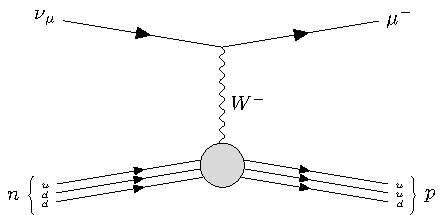
\includegraphics[width=.90\linewidth]{Images/Nu/feynman_ccqel.pdf}
		\caption{Quasi-elastic.}
	\end{subfigure}
	\begin{subfigure}{0.5\textwidth}
		\centering
		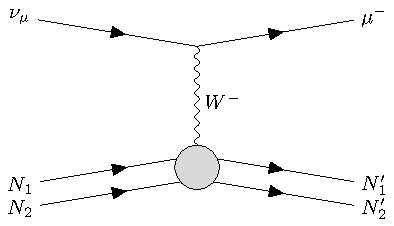
\includegraphics[width=.90\linewidth]{Images//Nu/feynman_ccmec.pdf}
		\caption{Coherent.}
	\end{subfigure}
	\begin{subfigure}{0.5\textwidth}
		\centering
		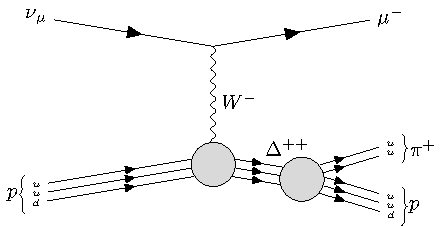
\includegraphics[width=.90\linewidth]{Images//Nu/feynman_ccres.pdf}
		\caption{Resonant.}
	\end{subfigure}
	\begin{subfigure}{0.5\textwidth}
		\centering
		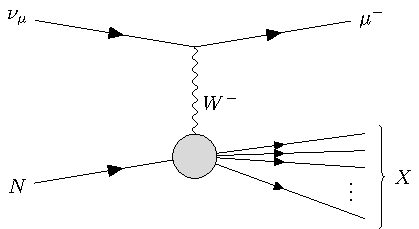
\includegraphics[width=.90\linewidth]{Images//Nu/feynman_ccdis.pdf}
		\caption{Deep inelastic.}
	\end{subfigure}
	\caption{Feynman diagrams of the four most relevant CC interactions to long baseline neutrino oscillation experiments.}
	\label{fig:neutrino_cc_interactions}
\end{figure}

% Neutrino-nucleon interactions
In the case of neutrino interactions with nuclei, at the energies relevant for long baseline oscillation experiments, around the $\mathrm{GeV}$-scale, the process is dominated by the interaction between the neutrino and a single nucleon within the nuclear medium. Figure \ref{fig:neutrino_cc_interactions} shows examples of the four most common neutrino CC interactions. In this diagrams $A$ indicated that the interaction happened with the nucles as a whole, whereas $N$ denotes a single nucleon.

\begin{figure}[t]
	\centering
	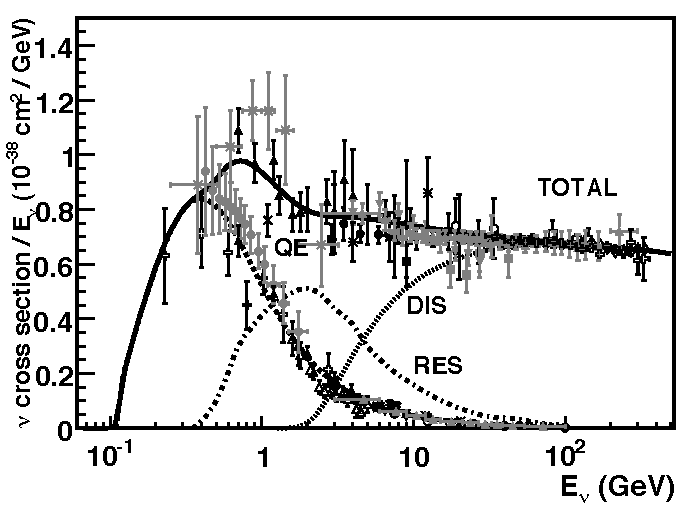
\includegraphics[width=.85\linewidth]{Images/Nu/numu_cc_cross_section.pdf}
	\caption[Total muon neutrino CC cross section per nucleon as a function of the neutrino energy.]{Total $\nu_{\mu}$ CC cross section per nucleon as a function of the neutrino energy. The contributions from the different channels are shown. Figure taken from Ref. \cite{Formaggio2012}.}
	\label{fig:numu_cc_cross_section}
\end{figure}

At low energies, below $1~\mathrm{GeV}$, quasi-elastic (QE) interactions dominate. In a CCQE interaction a neutrino (antineutrino) interacts with a neutron (proton), converting it into a proton (neutron) which is then ejected from the nucleus together with the resulting charged lepton. At energies above $1~\mathrm{GeV}$ the neutrino is able to excite the nucleon into a baryonic resonance, which promptly decays into a nucleon and a pion. These are the so-called resonant (RES) interactions. Neutrinos also interact with entire nucleus coherently, in the process known as coherent (COH) interaction. This kind of reactions also produce a single pion in the final state. At high neutrino energies, above $5~\mathrm{GeV}$, deep inelastic scattering (DIS) takes place. In these processes, the neutrino interacts with a single quark within the nucleon, breaking the nucleon and producing a hadronic shower.

Figure \ref{fig:numu_cc_cross_section} shows a compilation of measurements of the total $\nu_{\mu}$ CC cross section (see Ref. \cite{Formaggio2012} for the details of the different experimental results). Also shown are the contributions from the different interaction modes. The contribution of the CCCOH interaction is omitted, as it is negligible compared to the others. This shows how the interaction model needs to accurately predict the neutrino-nucleon cross section for the different interaction modes across a broad energy range, to obtain the correct relative contributions.

\begin{figure}[t]
	\centering
	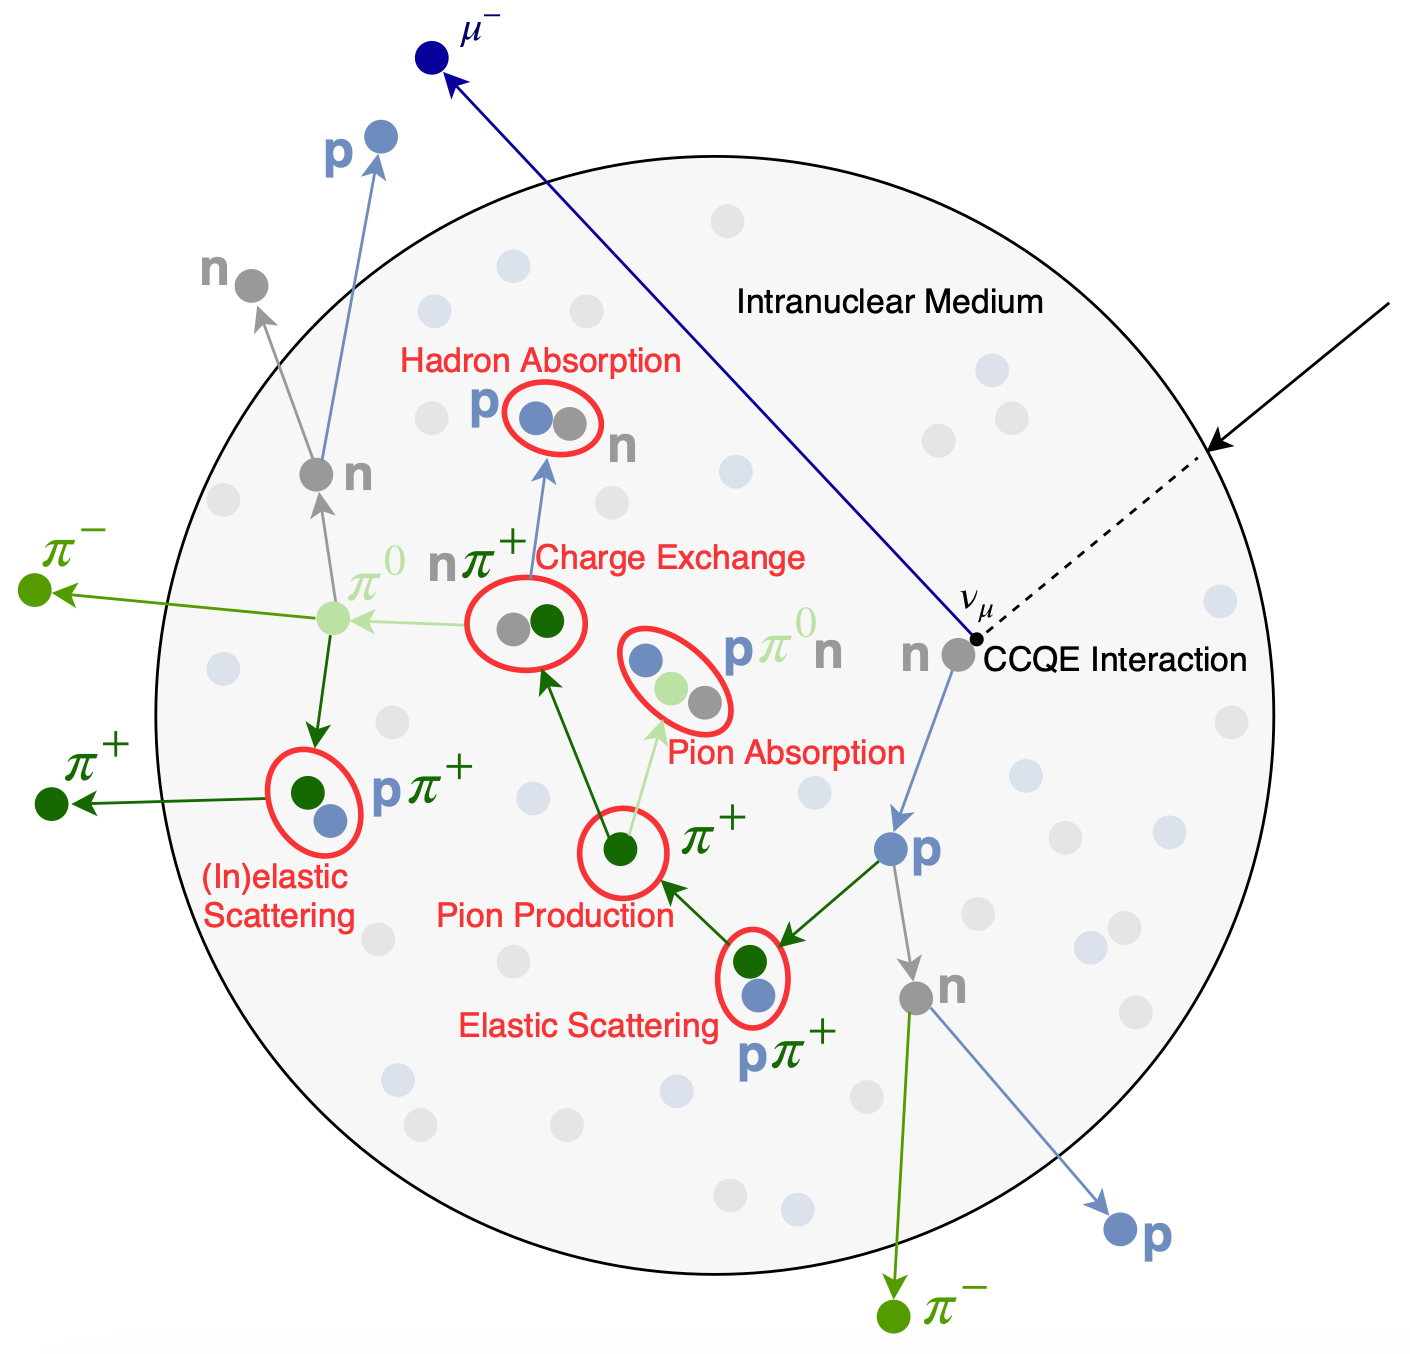
\includegraphics[width=.55\linewidth]{Images/Nu/lars_fsi.png}
	\caption[Schematic representation of a $\nu_{\mu}$ CCQE interaction with a neutron inside a nucleus.]{Schematic representation of a $\nu_{\mu}$ CCQE interaction with a neutron inside a nucleus. The reaction produces a muon and a proton, which travel through the nuclear medium. The outgoing proton undergoes various kinds of hadronic FSIs on its way out. Figure taken from Ref. \cite{Bathe-Peters2022}.}
	\label{fig:fsi_diagram}
\end{figure}

% Nuclear effects and FSI
Nuclear effects alter the neutrino cross section, as well as the multiplicities of the final state particles. Therefore, the interaction models need to account for the effects introduced by the nuclei. There are several models available to describe the initial state of the nucleus, like the relativistic Fermi gas model \cite{Smith1972}, spectral functions \cite{Nakamura2002} or the random phase approximation \cite{Pandey2014}. The other main effect that interaction models have to deal with are the so-called final state interactions (FSI). These are the interactions of the particles produced in the neutrino-nucleon scattering as they travel through the nuclear medium. Typically, the lepton exits the nucleus without interacting. However, hadrons tend to get scattered, absorbed or re-emitted. These effects are usually described by means of intra-nuclear cascade models \cite{Nikolakopoulos2022}. Figure \ref{fig:fsi_diagram} illustrates the effects of FSI on the observable particle content in the detector after a $\nu_{\mu}$ CCQE interaction.

% Experimental status
There exists a rich experimental programme dedicated to the measurement of neutrino cross sections. The list of such experiments in the recent years include MiniBooNE \cite{MiniBooNE2010}, MINERvA \cite{MINERvA2016}, MicroBooNE \cite{MicroBooNE2021} and SBND \cite{McConkey2018}. Additionally, thanks to their near detectors, long baseline experiments can perform cross section measurements. Some recent examples are NOvA \cite{Nova2021} or T2K \cite{T2K2019}. Future oscillation experiments will greatly benefit from these measurements, as the measurement of the oscillation parameters depends on the cross section modelling. However, there are alternative data-driven approaches to extract the oscillation probabilities without relying on a neutrino interaction model, which are planned to be explored in the next generation of experiments \cite{Scott2015,Hasnip2023}.
\chapter{The Deep Underground Neutrino Experiment}
\label{chapter:dune}

\begin{chapquote}{Frank Herbert, \textit{Dune}}
	Deep in the human unconscious is a pervasive need for a logical universe that makes sense. But the real universe is always one step beyond logic.
\end{chapquote}

%\noindent
The Deep Underground Neutrino Experiment (DUNE) is a next generation long-baseline neutrino oscillation experiment \cite{DUNE2020TDR1}. It will address several questions in neutrino physics, study neutrinos from astrophysical sources and search for beyond the standard model physics.

This Chapter reviews the main goals of DUNE, the operating principle of the LBNF beamline, the role that the near detector plays in the oscillation measurement, and the design of the far detector modules and their data acquisition (DAQ) system.

\section{Overview}

The main physics goals of DUNE are:
\begin{itemize}
	\item measure the neutrino mass hierarchy, the amount of CP violation in the leptonic sector and the $\theta_{23}$ octant,
	\item detect rare low energy neutrino events, like neutrinos from supernova bursts, and
	\item search for proton decay and other beyond the standard model phenomena.
\end{itemize}

The design of DUNE has been tailored with these goals in mind. It will consist of two neutrino detectors. A near detector (ND) complex will be placed at Fermilab, $574~\mathrm{m}$ downstream of the neutrino production point, whereas a larger far detector (FD) will be built in the Sandford Underground Research Facility (SURF), South Dakota, approximately $1300~\mathrm{km}$ away. Figure \ref{fig:dune} shows a simplified diagram with the various components of DUNE (not to scale).

\begin{figure}[t]
	\centering
	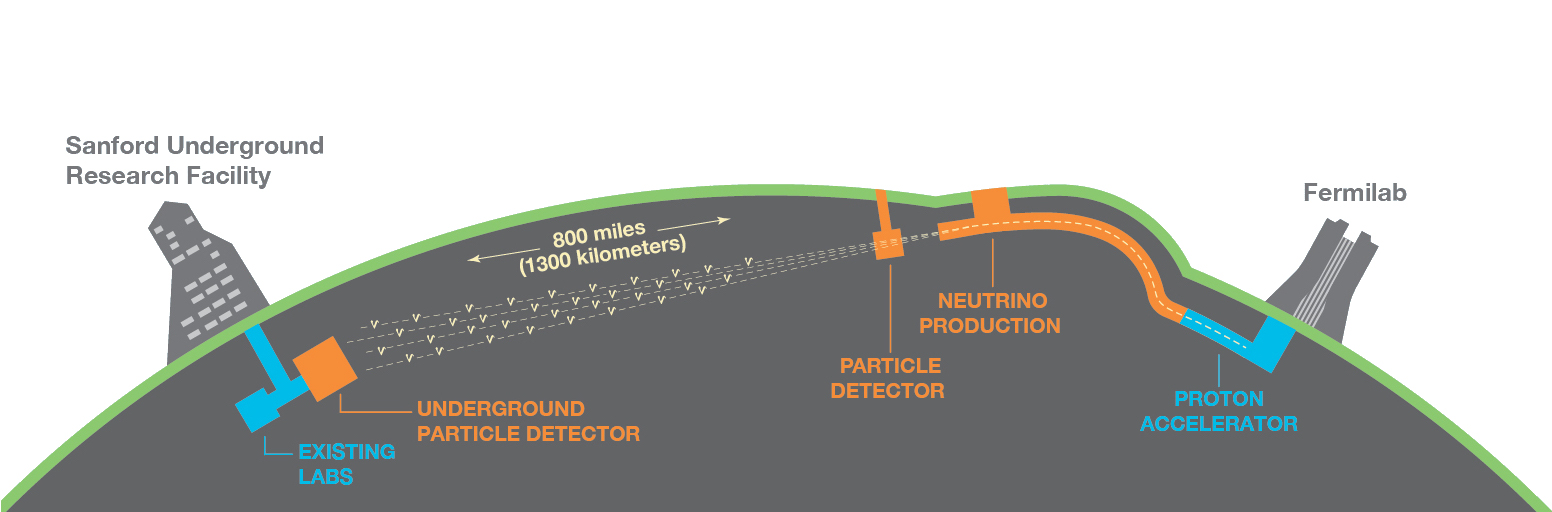
\includegraphics[width=0.9\linewidth]{Images/DUNE/FD/dune}
	\caption[Schematic diagram of the DUNE experiment and the LBNF beamline.]{Schematic diagram of the DUNE experiment and the LBNF beamline \cite{DUNE2020TDR1}.}
	\label{fig:dune}
\end{figure}

The beam neutrinos will be provided by the Long-Baseline Neutrino Facility (LBNF) beamline, the multi-megawatt wide-band neutrino beam planned for Fermilab. It will produce neutrinos travelling in the direction of SURF, with the capability to switch between neutrino and antineutrino mode.

Before arriving to the FD, the neutrino beam meets the ND complex, which serves as the experiment's control. The design of the DUNE ND is mainly driven by the needs of the oscillation physics programme, as its main role is to measure the unoscillated neutrino energy spectra. From these we can predict the unoscillated spectra at the FD, which can be compared to the spectra measured at the FD to extract the oscillation parameters. Additionally, the ND has a physics programme of its own, including cross section measurements and BSM physics searches.

The technology chosen for the FD modules of DUNE is the liquid Argon time projection chamber (LArTPC). Its four modules will record neutrino interactions from the accelerator-produced beam arriving at predictable times. As it also aims at recording rare and low energy events, like supernovae and solar neutrinos, the FD requires trigger schemes which can deal with both kinds of physics, and also maximum uptime.

\begin{table}[]
	\caption[Summary of the two-phased plan for DUNE.]{Summary of the two-phased plan for DUNE. Adapted from Ref. \cite{DUNE2022Snowmass}.}
	\centering
	\begin{tabular}{c|C{3.0cm}|C{3.0cm}|c}
	Parameter  & Phase I                     & Phase II		& Benefit \\[1mm] \hline
	\rule{0pt}{1.1\normalbaselineskip}FD mass    & $20 \ \mathrm{kt}$ fiducial & $40 \ \mathrm{kt}$ fiducial & FD statistics\\[1mm]
	Beam power & up to $1.2 \ \mathrm{MW}$   & $2.4 \ \mathrm{MW}$      & FD statistics  \\[1mm]
	ND config.  & ND-LAr, TMS, SAND           & ND-LAr, ND-GAr, SAND & Systematic constraints
	\end{tabular}
	\label{tab:dune_phases}
\end{table}

DUNE is planned to be built using a staged approach consisting on two phases, which are summarised in Tab. \ref{tab:dune_phases}. Phase I consists of a FD with $50\%$ of the total fiducial mass, a reduced version of the ND complex and a $1.2~\mathrm{MW}$ proton beam. It will be sufficient to achieve some early physics goals, like the determination of the neutrino mass ordering. For its Phase II, DUNE will feature the full four FD modules, a more capable ND and a $2.4~\mathrm{MW}$ proton beam. The physics milestones for the two phases are given in Tab. \ref{tab:dune_phases_physics}, in a staging scenario which assumes that Phase II is completed after 6 years of operation.

A summary of the DUNE science programme can be found in the DUNE FD Technical Design Report (TDR) Volume I \cite{DUNE2020TDR1}. For a detailed discussion on the two-phased approach the reader is referred to the DUNE Snowmass 2021 report \cite{DUNE2022Snowmass}.

\section{Physics goals of DUNE}

\begin{table}[]
	\caption[Exposure and time required to achieve the different physics milestones of the two phases.]{Exposure and time required to achieve the different physics milestones of the two phases. The predictions assume a Phase II staging scenario where FD modules 3 and 4 are deployed in years 4 and 6 and both the beam and ND are upgraded after 6 years. Adapted from Ref. \cite{DUNE2022Snowmass}.}
	\centering
	\begin{tabular}{c|c|C{3.0cm}|C{2.0cm}}
	Stage    & Physics milestone                                          & Exposure (kt-MW-years) & Years (staged) \\[3mm] \hline
	\rule{0pt}{1.1\normalbaselineskip}Phase I  & $5\sigma$ MO ($\delta_{CP} = -\pi/2$)                      & 16                     & 1-2            \\[1mm]
			 & $5\sigma$ MO ($100\%$ of the $\delta_{CP}$ values)         & 66                     & 3-5            \\[1mm]
			 & $3\sigma$ CPV ($\delta_{CP} = -\pi/2$)                     & 100                    & 4-6            \\[1mm] \hline
			 \rule{0pt}{1.1\normalbaselineskip}Phase II & $5\sigma$ CPV ($\delta_{CP} = -\pi/2$)                     & 334                    & 7-8            \\[1mm]
			 & $\delta_{CP}$ resolution of $10$ degrees ($\delta_{CP}=0$) & 400                    & 8-9            \\[1mm]
			 & $5\sigma$ CPV ($50\%$ of the $\delta_{CP}$ values)         & 646                    & 11             \\[1mm]
			 & $3\sigma$ CPV ($75\%$ of the $\delta_{CP}$ values)         & 936                    & 14             \\[1mm]
			 & $\mathrm{sin}^{2}(2\theta_{13})$ resolution of $0.004$       & 1079                   & 16            
	\end{tabular}
	\label{tab:dune_phases_physics}
\end{table}

As noted in the literature (see for instance Ref. \cite{deSalas2020} for a review), the parameter space of the neutrino oscillation phenomena within the three-flavour picture is quite constrained by current experimental data. However, there are still crucial open questions, like the mass ordering, the value of $\delta_{CP}$ or the $\theta_{23}$ octant. One of the main goals of DUNE is to determine precisely the values of these parameters \cite{DUNE2020TDR2}.

To address these questions DUNE can look to the subdominant oscillation channel $\nu_{\mu} \rightarrow \nu_{e}$ ($\bar{\nu}_{\mu} \rightarrow \bar{\nu}_{e}$) and study the energy dependence of the $\nu_{e}$ ($\bar{\nu}_{e}$) appearance probability. When we focus on the antineutrino channel $\bar{\nu}_{\mu} \rightarrow \bar{\nu}_{e}$ there is a change in the sign of $\delta_{CP}$, thus introducing CP-violation. Moreover, due to the fact that there are no positrons in the composition of the Earth, there is a sign difference for the matter effect contribution when looking to the antineutrino channel. This asymmetry is proportional to the baseline length $L$ and is sensitive to the sign of $\Delta m^{2}_{31}$, and thus to the neutrino mass ordering.

Another of the main physics goals of DUNE is the search for baryon-number violating processes. Specifically, it will try to answer the question of whether protons are stable or not. There is no symmetry argument that forbids protons from decaying, but its apparent stability seems to suggest that baryon number is conserved \cite{Super-Kamiokande2009}. However, proton decay is a usual feature of grand-unified theories, where electromagnetic, weak and strong interactions are unified above a certain energy scale \cite{Raby2006}.

As the energy deposition scale for this kind of searches is nearly the same as the one for long-baseline neutrino oscillations, DUNE will be able to look for them. It has several advantages over other experiments, such as excellent imaging and particle identification, which can be translated into lower backgrounds.

The last of the main objectives of DUNE is the detection of neutrinos originated in supernovae explosions, what is called a supernova neutrino burst (SNB). These neutrinos carry with them information about the core-collapse process, from the progenitor to the explosion and the remnant; but also may have information about new exotic physics. So far, the only neutrino events ever recorded from such a process were a few dozens of $\bar{\nu}_{e}$ events from the 1987A supernova located in the Magellanic Cloud, $50~\mathrm{kpc}$ away from Earth \cite{Kamiokande-II1987, Bionta1987}.

DUNE aims to collect SNB events. Although these are quite rare, as the expected supernovae explosion events are about one every few decades for our galaxy and Andromeda, the long lifetime of the experiment (around a couple of decades as well) makes it reasonable to expect some. Nowadays the main sensitivity to SNB of most experiments is to the $\bar{\nu}_{e}$ flux through inverse beta decay. One of the advantages of DUNE is its expected sensitivity to MeV-scale $\nu_{e}$ events, since the dominant channel will be $\nu_{e}$ CC scattering.

Moreover, due to the stringent requirements that the main physics goals set for DUNE, it will allow also to perform searches for all kind of BSM physics. Among others, DUNE will be able to look for: active-sterile neutrino mixing, non-unitarity of the PMNS matrix, non-standard interactions, Lorentz and CPT violations, neutrino trident production, light-mass DM, boosted DM, and heavy neutral leptons. The reader is referred to the DUNE FD TDR Volume II \cite{DUNE2020TDR2} for a full discussion of the physics scope of DUNE.

\begin{figure}[t]
	\centering
	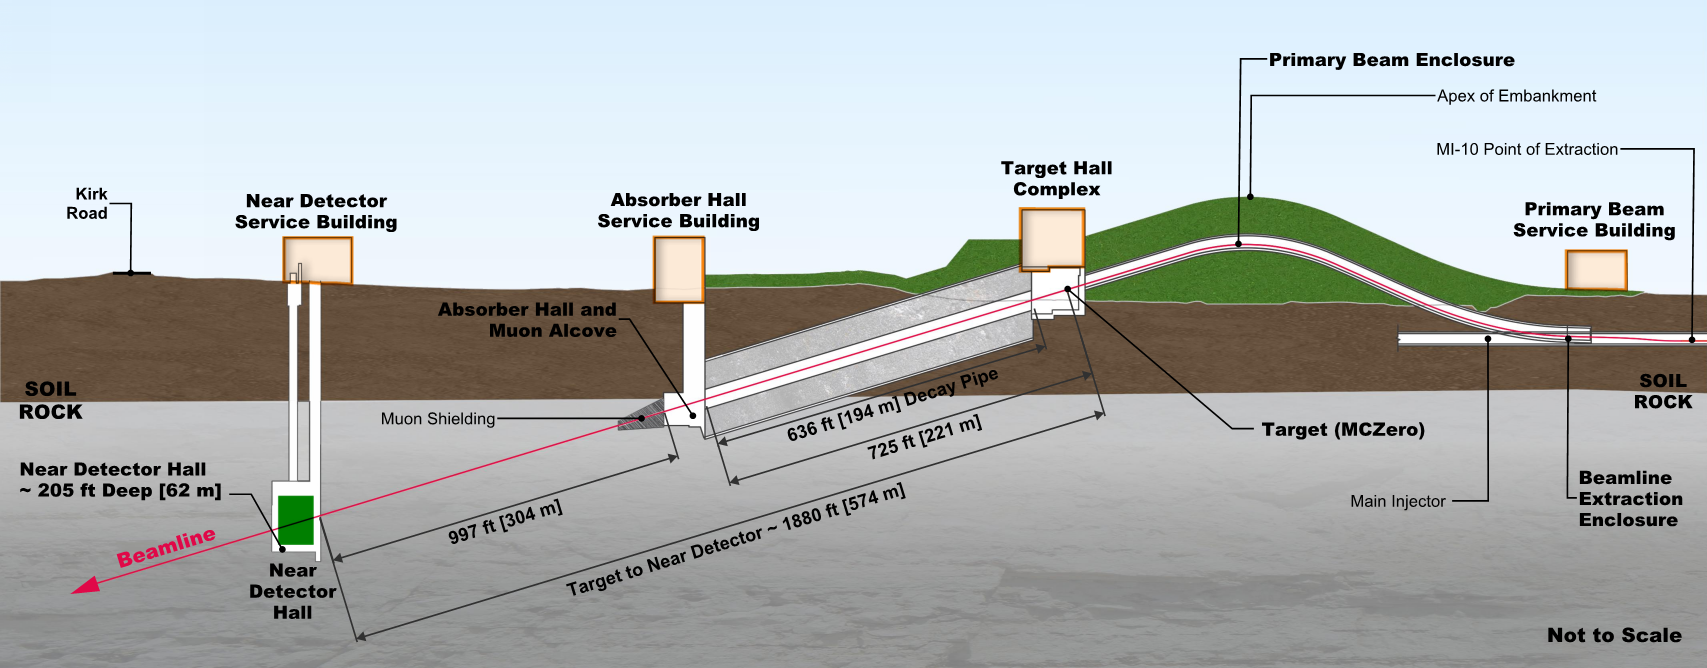
\includegraphics[width=0.95\linewidth]{Images/DUNE/LBNF/beamline-sideview}
	\caption[Schematic longitudinal section of the LBNF beamline at Fermilab.]{Schematic longitudinal section of the LBNF beamline at Fermilab (not to scale). Figure taken from Ref. \cite{DUNE2016CDR3}.}
	\label{fig:lbnf_beamline}
\end{figure}

\section{LBNF beamline}

The LBNF project is responsible for producing the neutrino beam for the DUNE detectors. A detailed discussion of the LBNF programme can be found in the DUNE/LBNF CDR Volume III \cite{DUNE2016CDR3}.

A schematic diagram of the longitudinal section of the LBNF beamline is shown in Fig. \ref{fig:lbnf_beamline}. First, a beam of $60-120~\mathrm{GeV}$ protons is extracted from the Fermilab Main Injector. This beam is aimed towards the target area, where it collides with a cylindrical graphite target to produce charged pions and kaons.

The diffuse, secondary beam of particles is focused by a pair of magnetic horns. These select the positively charged particles when operated in Forward Horn Current (FHC) mode, or the negatively charged ones when the current is reversed, also known as Reverse Horn Current (RHC) mode. The focused secondary beam then enters a $194~\mathrm{m}$ decay pipe where the pions and kaons will predominantly produce $\mu^{+}\nu_{\mu}$ pairs when in FHC mode (or $\mu^{-}\bar{\nu}_{\mu}$ in RHC mode).

At the end of the decay pipe a hadron absorber removes the undecayed hadrons and muons from the beam, which reduces the $\nu_{e}$ ($\bar{\nu}_{e}$) and $\bar{\nu}_{\mu}$ ($\nu_{\mu}$) contamination  coming from the $\mu^{+}$ ($\mu^{-}$) decays. The resulting neutrino flux at the FD is shown in Fig. \ref{fig:dune_fd_flux}, both for FHC (left) and RHC (right) modes. These predictions show the intrinsic $\overset{\brabarb}{\nu}_{e}$ contamination and wrong sign component from wrong sign and neutral meson decays, as well as muons decaying before reaching the absorber.

\begin{figure}[h!]
	\begin{subfigure}{0.49\textwidth}
		\centering
		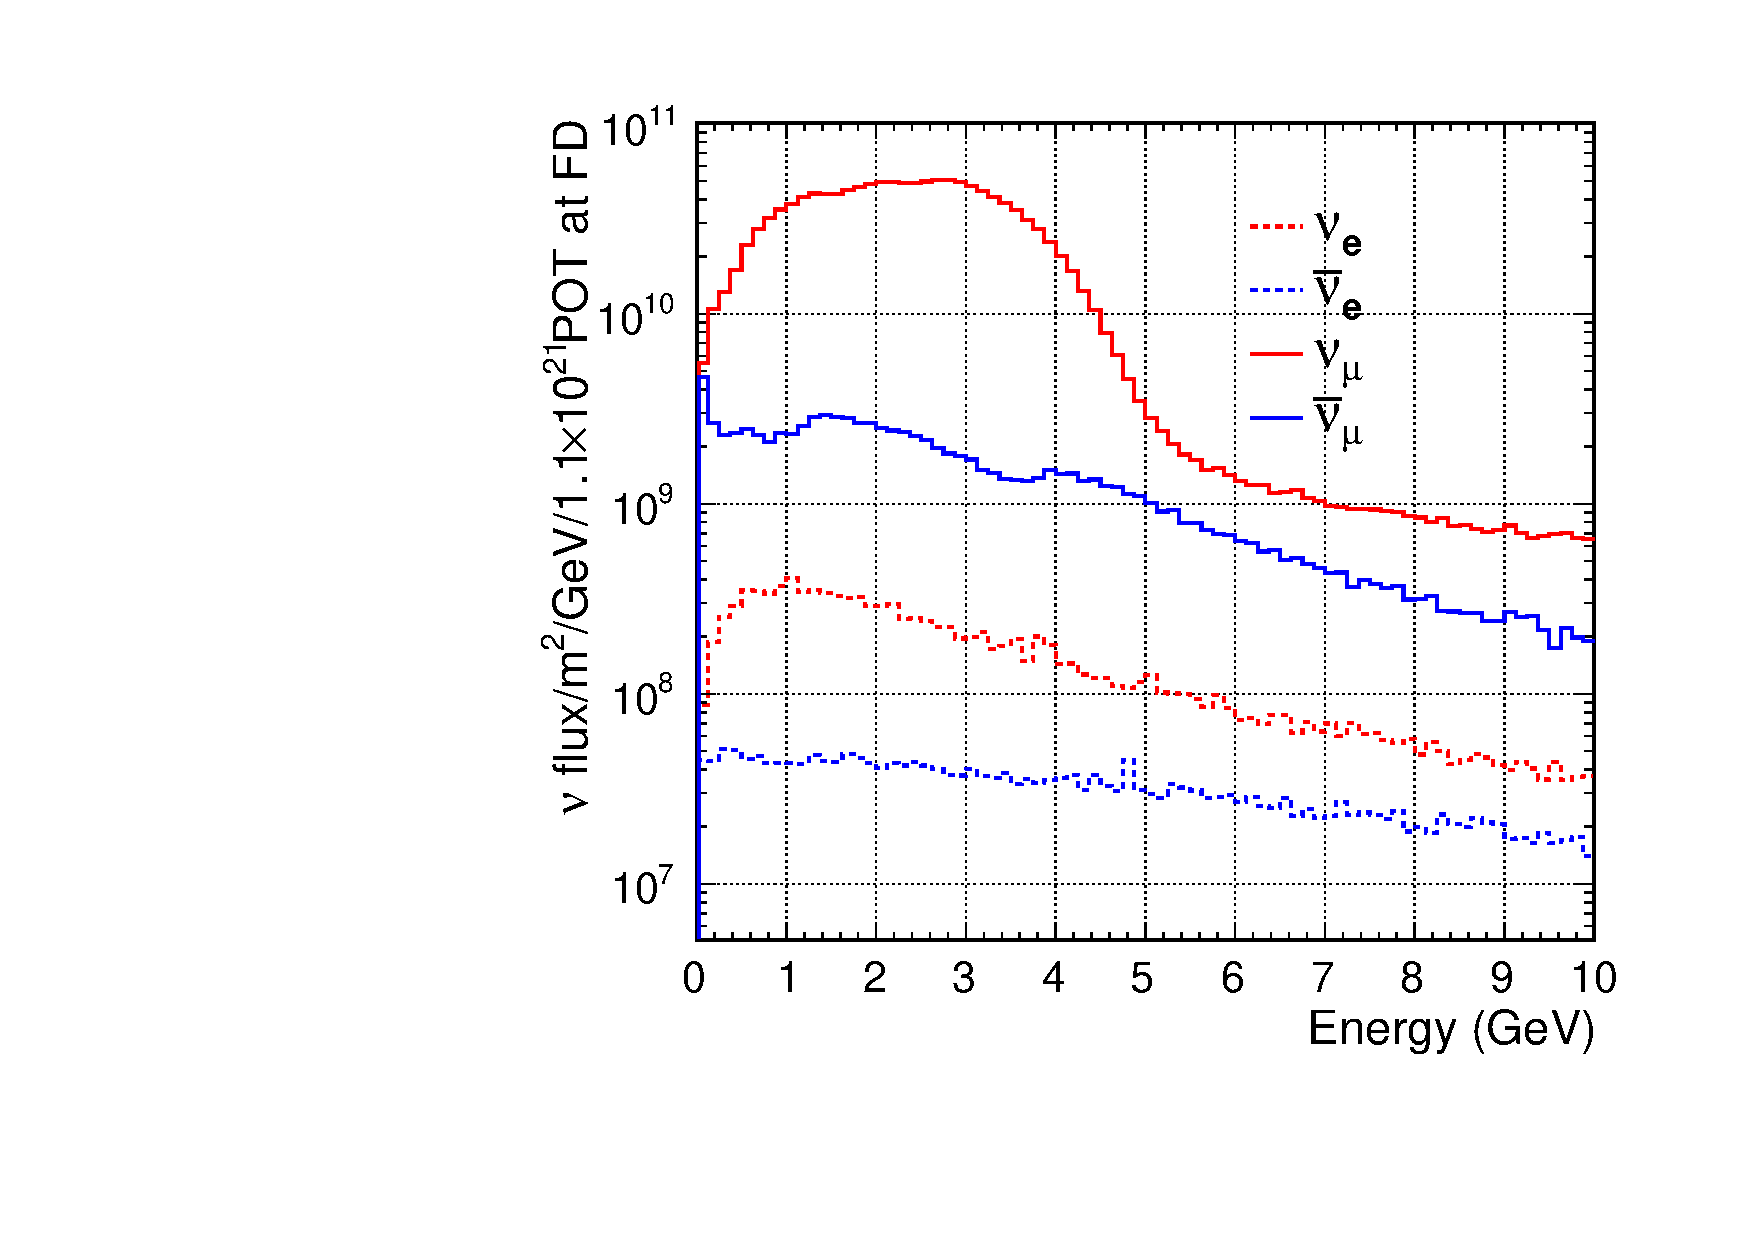
\includegraphics[width=.99\linewidth]{Images/DUNE/LBNF/dune_neutrino_fd_log}
	\end{subfigure}
	\begin{subfigure}{0.49\textwidth}
		\centering
		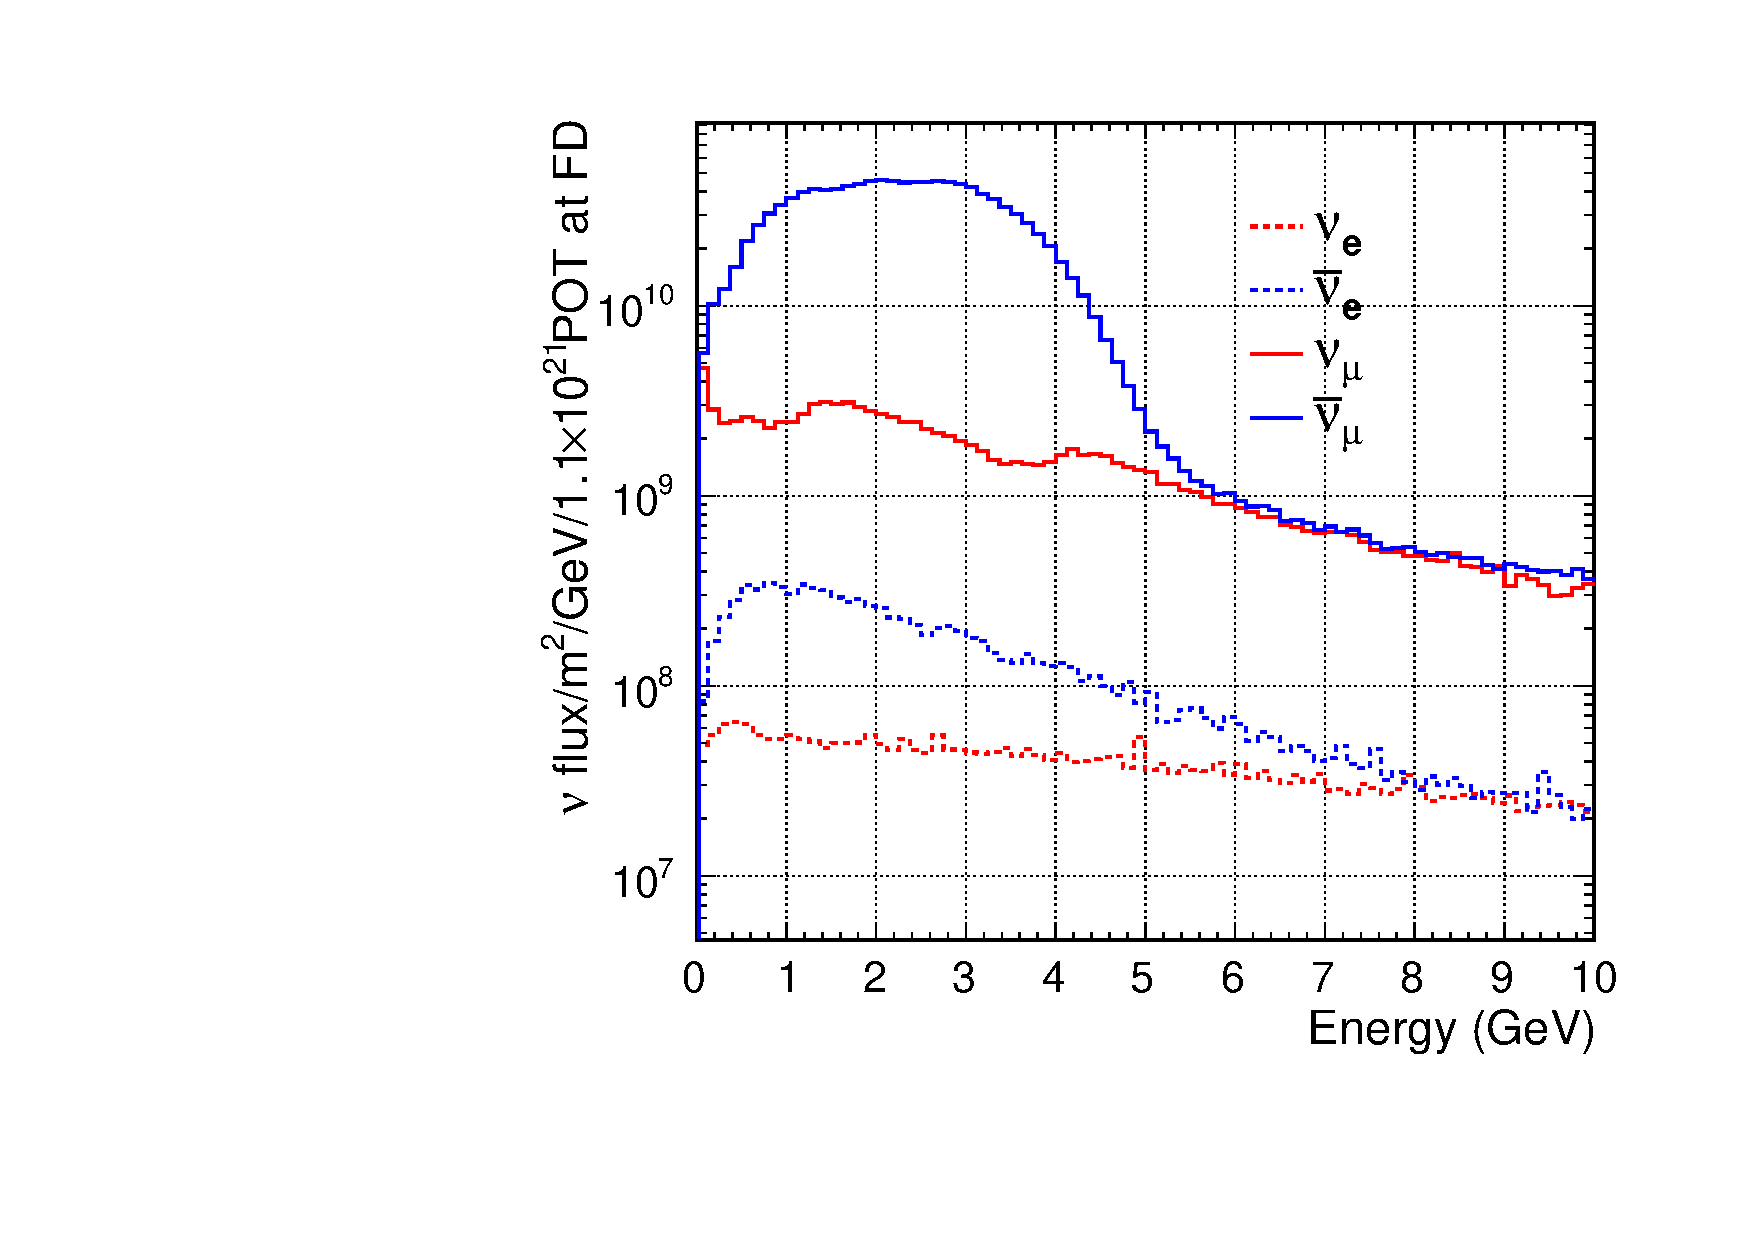
\includegraphics[width=.99\linewidth]{Images/DUNE/LBNF/dune_antineutrino_fd_log}
	\end{subfigure}
	\caption[Predicted neutrino fluxes at the FD in FHC mode and RHC mode.]{Predicted neutrino fluxes at the FD in FHC mode (left panel) and RHC mode (right panel). Figures taken from Ref. \cite{DUNE2020TDR2}.}
	\label{fig:dune_fd_flux}
\end{figure}

\section{Near Detector}

To estimate the oscillation parameters we measure the neutrino energy spectra at the FD. This reconstructed energy arises from a convolution of the neutrino flux, cross section, detector response and the oscillation probability. Using theoretical and empirical models to account for the other effects, one can extract the oscillation probability using the measurement. However, these models have associated a number of uncertainties that are then propagated to the oscillation parameters.

\begin{figure}[t]
	\centering
	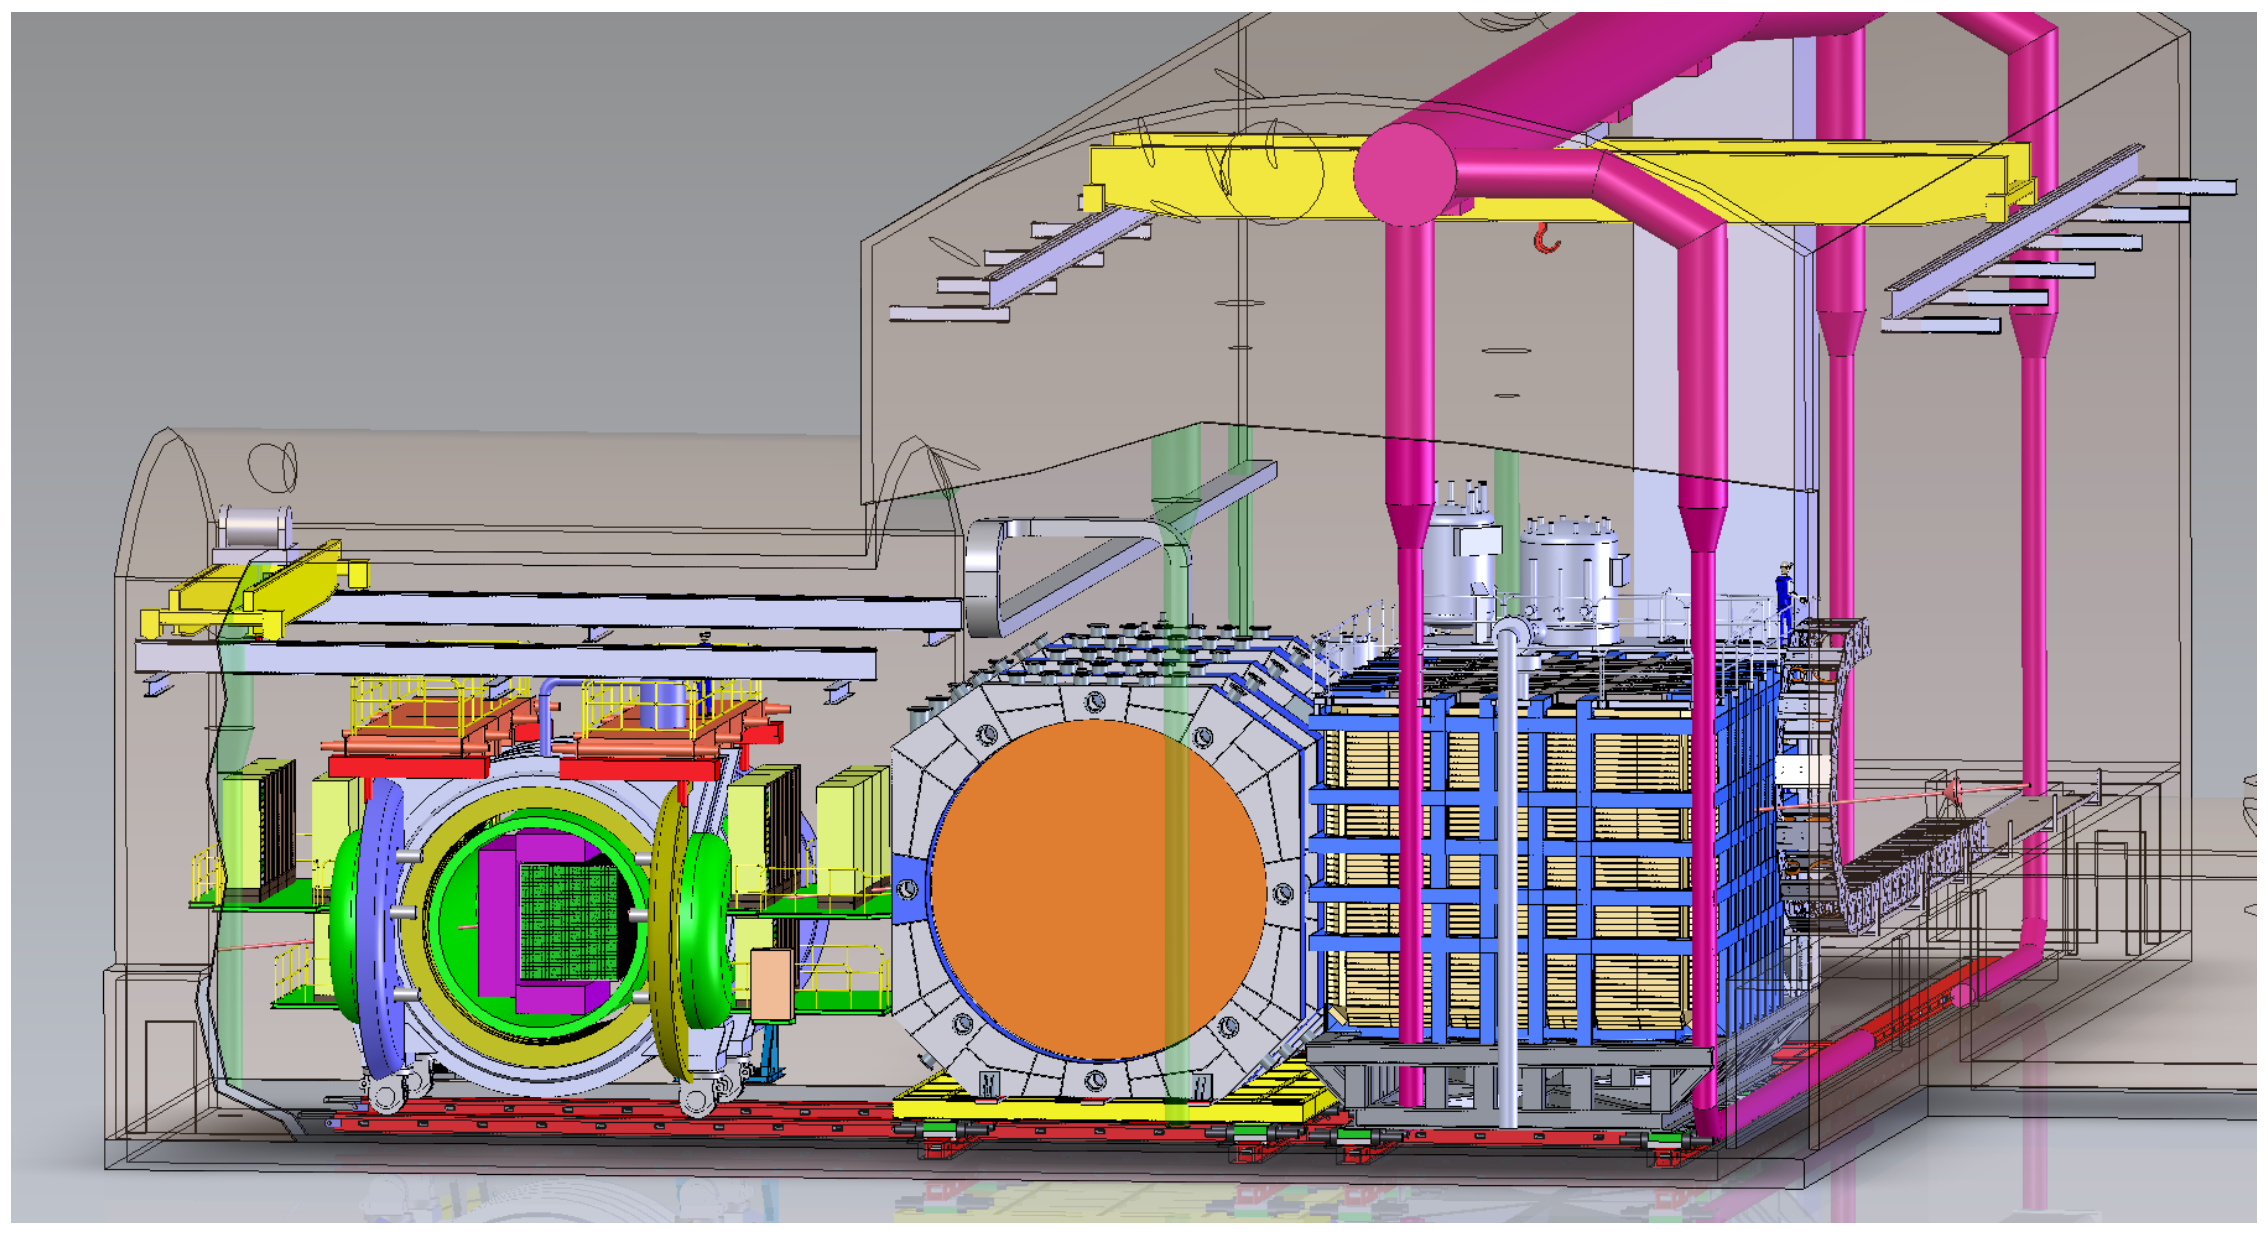
\includegraphics[width=0.95\linewidth]{Images/DUNE/ND/nd_hall}
	\caption[Representation of the ND hall in Phase II, showing the different subcomponents.]{Representation of the ND hall in Phase II, showing the different subcomponents. From right to left, in the direction of the beam, we have ND-LAr, ND-GAr and SAND. Figure taken from Ref. \cite{DUNE2021NDCDR}.}
	\label{fig:dune_nd}
\end{figure}

One of the main roles of the ND is to measure the neutrino interaction rates before the oscillation effects become relevant, i.e. close to the production point. By measuring the $\nu_{\mu}$ and $\nu_{e}$ energy spectra, and that of their corresponding antineutrinos, at the ND we can constrain the model uncertainties. A complete cancellation of the uncertainties when taking the ratio between the FD and ND measurements is not possible, as that would require both detectors to have identical designs and the neutrino fluxes seen by them to be the same. Because of the distance, the flux probed by the FD will have a different energy and flavour composition than that at the ND, as neutrinos oscillate and the beam spreads. The differences in the flux also determine the design of the detectors, therefore the ND is limited in its capability to match the FD design.

Nevertheless, having a highly capable ND, DUNE can minimise the systematic uncertainties affecting the observed neutrino energy. The ND data can be used to tune the model parameters by comparison with the prediction. Then, one uses the tuned model to predict the unoscillated FD spectra. Comparing the prediction with the measured spectra it is possible to extract the oscillation parameters.

\begin{comment}
	Another requirement for the ND is that it must reduce the impact of the cross section uncertainties on the measurement of the neutrino spectra. In other words, it needs to measure neutrino interactions much more accurately than the FD. This requires a better particle identification and energy reconstruction capabilities.
\end{comment}

\begin{figure}[t]
	\centering
	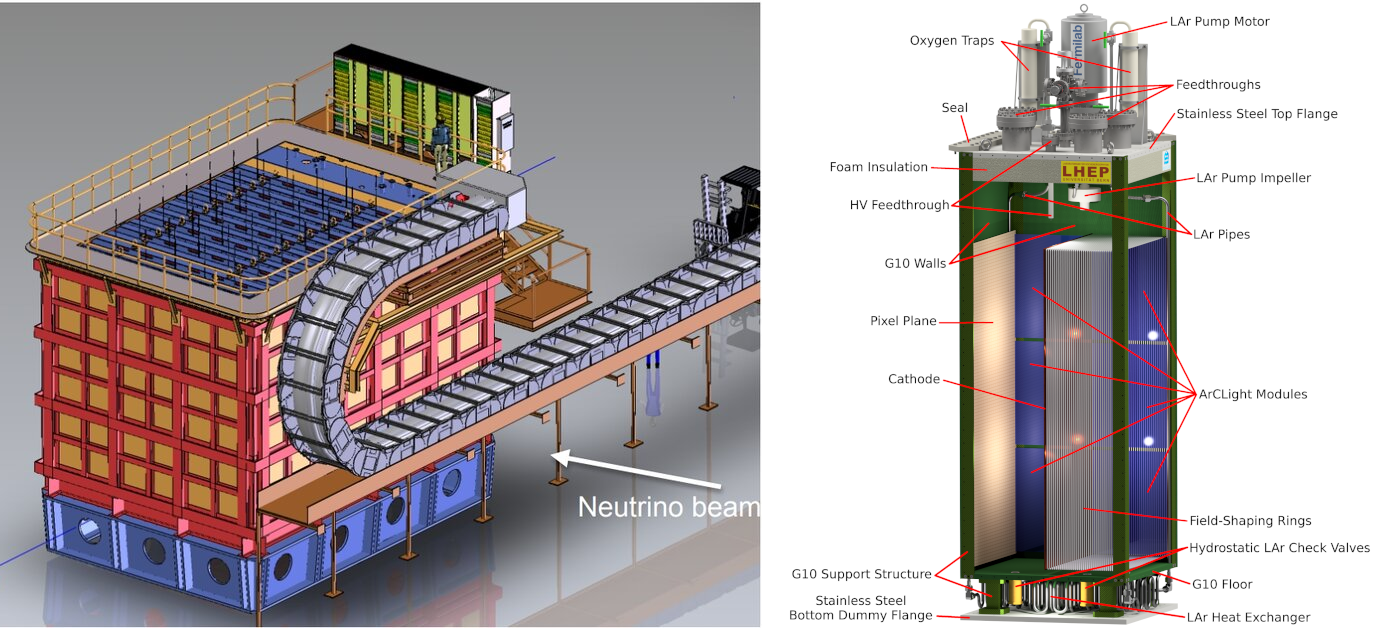
\includegraphics[width=0.99\linewidth]{Images/DUNE/ND/nd_lar_mod}
	\caption[Schematic representation of the external components of ND-LAr, including the cryostat and the PRISM movable system and detailed drawing of one ArgonCube module.]{Schematic representation of the external components of ND-LAr, including the cryostat and the PRISM movable system (left) and detailed drawing of one ArgonCube module (right). Figure adapted from Ref. \cite{DUNE2020TDR1}.}
	\label{fig:dune_nd_lar}
\end{figure}

Additionally, the ND will have a physics programme of its own. In particular, it will measure neutrino cross sections that will then be used to constrain the model used in the long-baseline oscillation analysis. It will also be used to search for BSM phenomena such as heavy neutral leptons, dark photons, millicharged particles, etc.

The DUNE ND can be divided in three main components, a LArTPC known as ND-LAr, a magnetised muon spectrometer, which will be the Temporary Muon Spectrometer (TMS) in Phase I and ND-GAr in Phase II, and the System for on-Axis Neutrino Detection (SAND). The layout of the Phase II DUNE ND can be seen in Fig. \ref{fig:dune_nd}. The first two components of the ND will be able to move off-axis, in what is called the Precision Reaction-Independent Spectrum Measurement (PRISM) concept. More details on the purpose and design of the ND can be found in the DUNE ND Conceptual Design Report (CDR) \cite{DUNE2021NDCDR}.

\subsection{ND-LAr}

\begin{figure}[t]
	\centering
	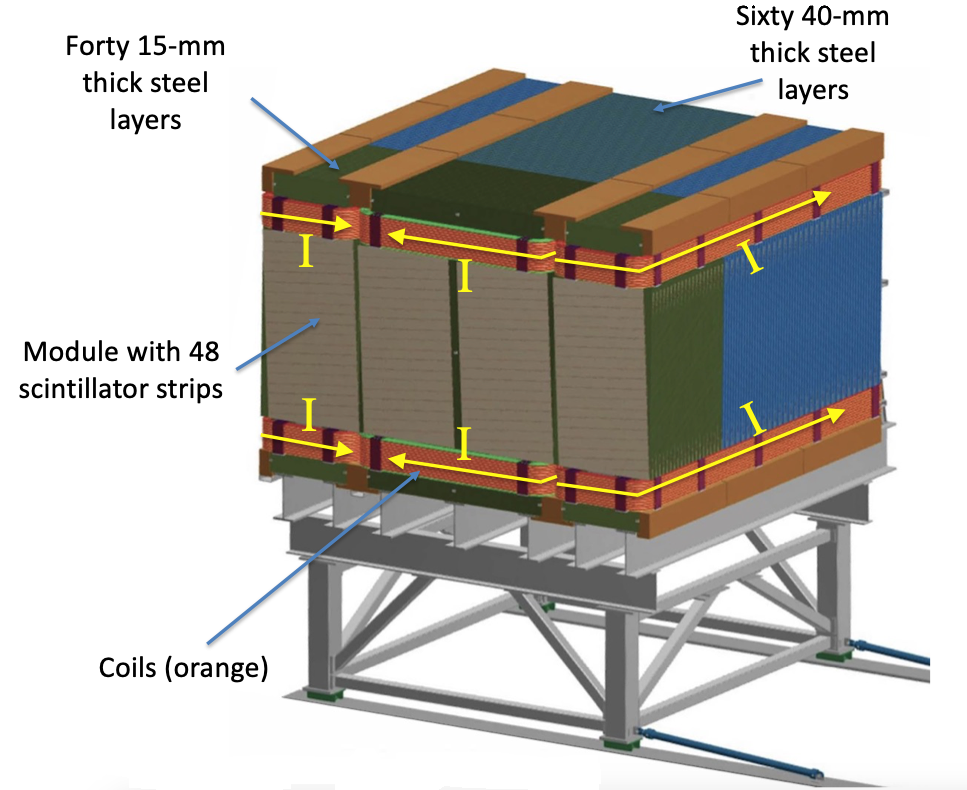
\includegraphics[width=0.65\linewidth]{Images/DUNE/ND/nd_tms}
	\caption[Schematic view of the TMS detector, highlighting its main parts.]{Schematic view of the TMS detector, highlighting its main parts. Figure adapted from Ref. \cite{Nehm2024}.}
	\label{fig:dune_tms}
\end{figure}

ND-LAr is a LArTPC, as the ND needs a LAr component to reduce cross section and detector systematic uncertainties in the oscillation analysis. However, its design differs significantly from those proposed for the FD modules. Because of the high event rates at the ND, approximately $55$ neutrino interaction events per $10~\mu\mathrm{s}$ spill, ND-LAr will be built in a modular way. Each of the modules, based on the ArgonCube technology, is a fully instrumented, optically isolated TPC with a pixelated readout \cite{Asaadi2019}. The pixelisation allows for a fully 3D reconstruction and the optical isolation reduces the problems due to overlapping interactions. Figure \ref{fig:dune_nd_lar} shows a representation of the external parts of ND-LAr (left) and a detailed diagram of an ArgonCube module (right).

With a fiducial mass of $67~\mathrm{t}$ and dimensions $7~\mathrm{m} \ (\text{w}) \times 3~\mathrm{m} \ (\text{h}) \times 5~\mathrm{m} \ (\text{l})$, ND-LAr will be able to provide high statistics and contain the hadronic systems from the beam neutrino interactions, but muons with a momentum higher than $0.7~\mathrm{GeV}/c$ will exit the detector.

\begin{figure}[t]
	\centering
	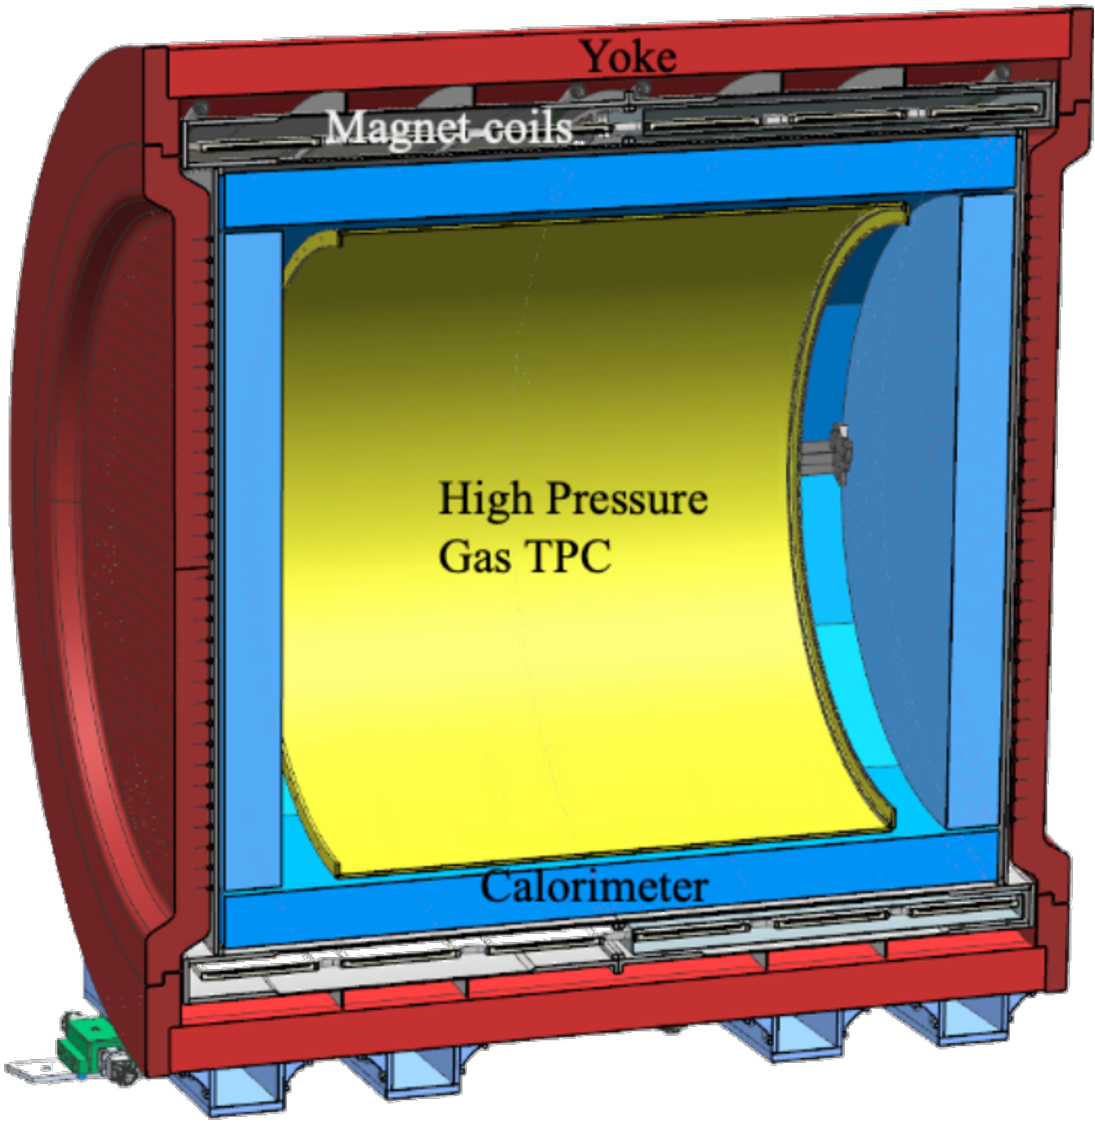
\includegraphics[width=0.45\linewidth]{Images/DUNE/ND/nd_gar}
	\caption[Cross section of the ND-GAr geometry, showing the HPgTPC, ECal and magnet.]{Cross section of the ND-GAr geometry, showing the HPgTPC, ECal and magnet. Figure adapted from Ref. \cite{DUNE2024Phase2}.}
	\label{fig:dune_nd_gar}
\end{figure}

\subsection{TMS/ND-GAr}

To accurately estimate the neutrino energy, the momentum of the outgoing muons needs to be determined. That is the reason why a muon spectrometer is needed downstream of ND-LAr.

In Phase I that role will be fulfilled by TMS. It is a magnetised sampling calorimeter, with alternating steel and plastic scintillator layers. Figure \ref{fig:dune_tms} shows a schematic view of the TMS detector. The magnetic field allows a precise measurement of the sign of the muon, so one can distinguish between neutrino and antineutrino interactions.

After the Phase II upgrade, TMS will be replaced with a more capable near detector. The current technology considered is ND-GAr. This detector is a magnetised, high-pressure gaseous argon (GAr) TPC (often denoted as HPgTPC) surrounded by an electromagnetic calorimeter (ECal) and a muon tagger. A cross section of its geometry can be seen in Fig. \ref{fig:dune_nd_gar}. ND-GAr will be able to measure the momenta of the outgoing muons while also detect neutrino interactions inside the GAr volume. This allows ND-GAr to constrain the systematic uncertainties even further, as it will be able to accurately measure neutrino interactions at low energies thanks to the lower tracking thresholds of the GAr.

\begin{figure}[t]
	\centering
	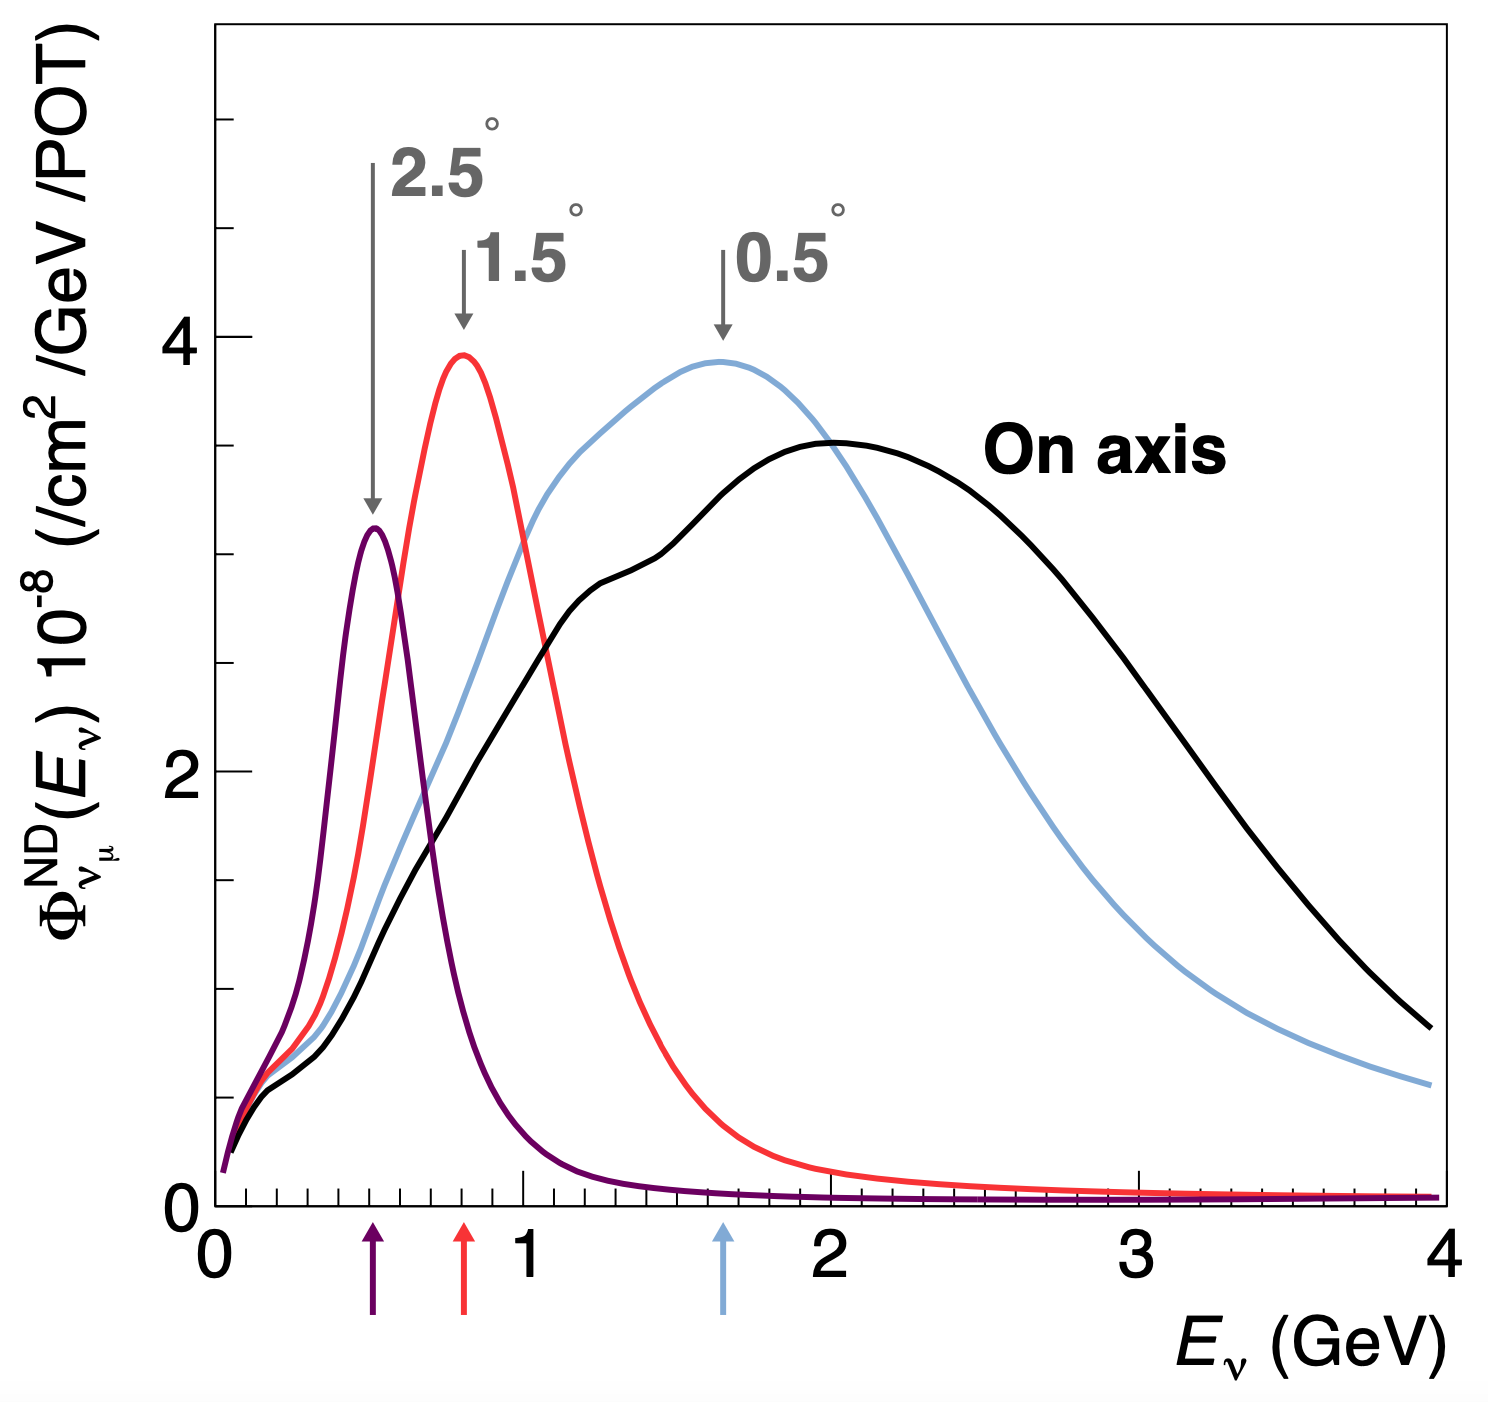
\includegraphics[width=0.55\linewidth]{Images/DUNE/ND/prism_spectra}
	\caption[Predicted beam muon neutrino flux at the ND location for different off-axis positions.]{Predicted beam muon neutrino flux at the ND location for different off-axis positions. Figure taken from Ref. \cite{DUNE2021NDCDR}.}
	\label{fig:dune_prism}
\end{figure}

\subsection{PRISM}

In general, the observed peak neutrino energy of a neutrino beam decreases as the observation angle with respect to the beam direction increases. This feature has been used in other long-baseline neutrino experiments, like T2K ($2.5^{\circ}$ off-axis) and NOvA ($0.8^{\circ}$ off-axis), to achieve narrower energy distributions. The DUNE PRISM concept exploits this effect using a movable ND. Within PRISM both ND-LAr and the muon spectrometer (TMS in Phase I and ND-GAr in Phase II) can be moved up to $3.2^{\circ}$ off-axis, equivalent to moving the detectors $30.5~\mathrm{m}$ laterally through the ND hall.

This allows us to record additional data samples with different energy compositions. Figure \ref{fig:dune_prism} compares the on-axis muon neutrino flux at the ND with the fluxes at different off-axis positions. As the off-axis position increases the neutrino flux becomes closer to a monoenergetic beam with a lower peak energy. These samples can be used to perform a data-driven determination of the relation between true and reconstructed neutrino energy, to reduce the dependence on the interaction model. The off-axis samples are linearly combined to produce a narrow Gaussian energy distribution centered on a target true energy. From the combination coefficients one can build a sample of reconstructed neutrino events that will determine the energy mapping.

The PRISM samples will also be used to form a flux at the ND location similar in shape to the oscillated flux measured by the FD. This method can be used to extract the oscillation parameters with minimal input from the neutrino interaction model \cite{Hasnip2023}.

\subsection{SAND}

The role of SAND is to monitor the beam stability by measuring the on-axis neutrino energy spectra. As the PRISM programme requires that ND-LAr and its downstream muon spectrometer spend about half of the time in off-axis positions, it is not possible to monitor the stability of the beam with the movable detectors. Moreover, for the success of PRISM it is essential to have a stable beam configuration, or at least a quick assessment and modeling of the distortions.

The SAND detector is magnetised, and features an inner low density tracker, a LAr target with optical readout and a surrounding sampling calorimeter.

\section{A More Capable Near Detector}\label{sec:mcnd}

In DUNE Phase II, a more capable near detector is needed to achieve the ultimate physics goals of the experiment. The current leading proposal for this detector is ND-GAr. As mentioned previously, it will fulfill the role of TMS, measuring the momentum and sign of the charged particles exiting ND-LAr. Additionally, it will be able to measure neutrino interactions inside the HPgTPC, achieving lower energy thresholds than those of the ND and FD LArTPCs. It will also provide a uniform event acceptance, similar to the FD, which could not be achieved by ND-LAr + TMS. By doing so, ND-GAr will allow to constrain the relevant systematic uncertainties for the LBL analysis even further. A detailed discussion on the requirements, design, performance and physics of ND-GAr can be found in the DUNE ND CDR \cite{DUNE2021NDCDR} and the ND-GAr white paper \cite{DUNE2022GArWhite}.

\subsection{Requirements}

The primary requirement for ND-GAr is to measure the momentum and charge of muons from $\nu_{\mu}$ and $\bar{\nu}_{\mu}$ CC interactions in ND-LAr, in order to measure their energy spectrum. To achieve the sensitivity to the neutrino oscillation parameters described in the DUNE FD TDR Volume II \cite{DUNE2020TDR2}, ND-GAr should be able to constrain the muon energy within a $1\%$ uncertainty or better.

Another requirement for ND-GAr is the precise measurement of neutrino interactions on argon for the energies relevant to the neutrino oscillation program. The goal is to constrain the cross section systematic uncertainties in the regions of phase space that are not accessible to ND-LAr. This requires the kinematic acceptance for muons in ND-GAr to exceed that of ND-LAr, being comparable to the one observed in the FD.

ND-GAr should also be able to help establishing the relationship between true and reconstructed energy from neutrino interactions on argon, being sensitive to particles that are not observed or may be misidentified in ND-LAr. In particular, ND-GAr needs to have low tracking thresholds in order to measure the spectrum of pions and protons produced in final-state interactions (FSI). It also must be able to accurately measure the pion multiplicity in 1, 2 and 3 pions final states, to inform the pion mass correction in the LArTPCs.

\subsection{Reference design}\label{subsec:ndgar_design}

The final design of ND-GAr is still under preparation. However, a preliminary baseline design was in place at the time of the ND CDR. This section summarises the main features of that design, as it is also the one used by default in our simulation. The different options under consideration for the ND-GAr design are further discussed in the DUNE Phase II white paper \cite{DUNE2024Phase2}.

\subsubsection{HPgTPC}

The reference design for the ND-GAr HPgTPC follows closely that of the ALICE TPC \cite{ALICE2006}. It is a cylinder with a central high-voltage cathode, generating the electric field for the two drift volumes, with a maximum drift distance of $2.5~\mathrm{m}$ each. The anodes will be instrumented with charge readout chambers. The original design repurposed the multi-wire proportional readout chambers (MWPCs) of ALICE. However, some of the current R\&D efforts focus on a gas electron multiplier (GEM) \cite{Sauli1997} option instead. Figure \ref{fig:alice_tpc} shows a schematic diagram of the ALICE TPC design. The basic ND-GAr geometry will resemble this, except for the inner field cage.

\begin{figure}[t]
	\centering
	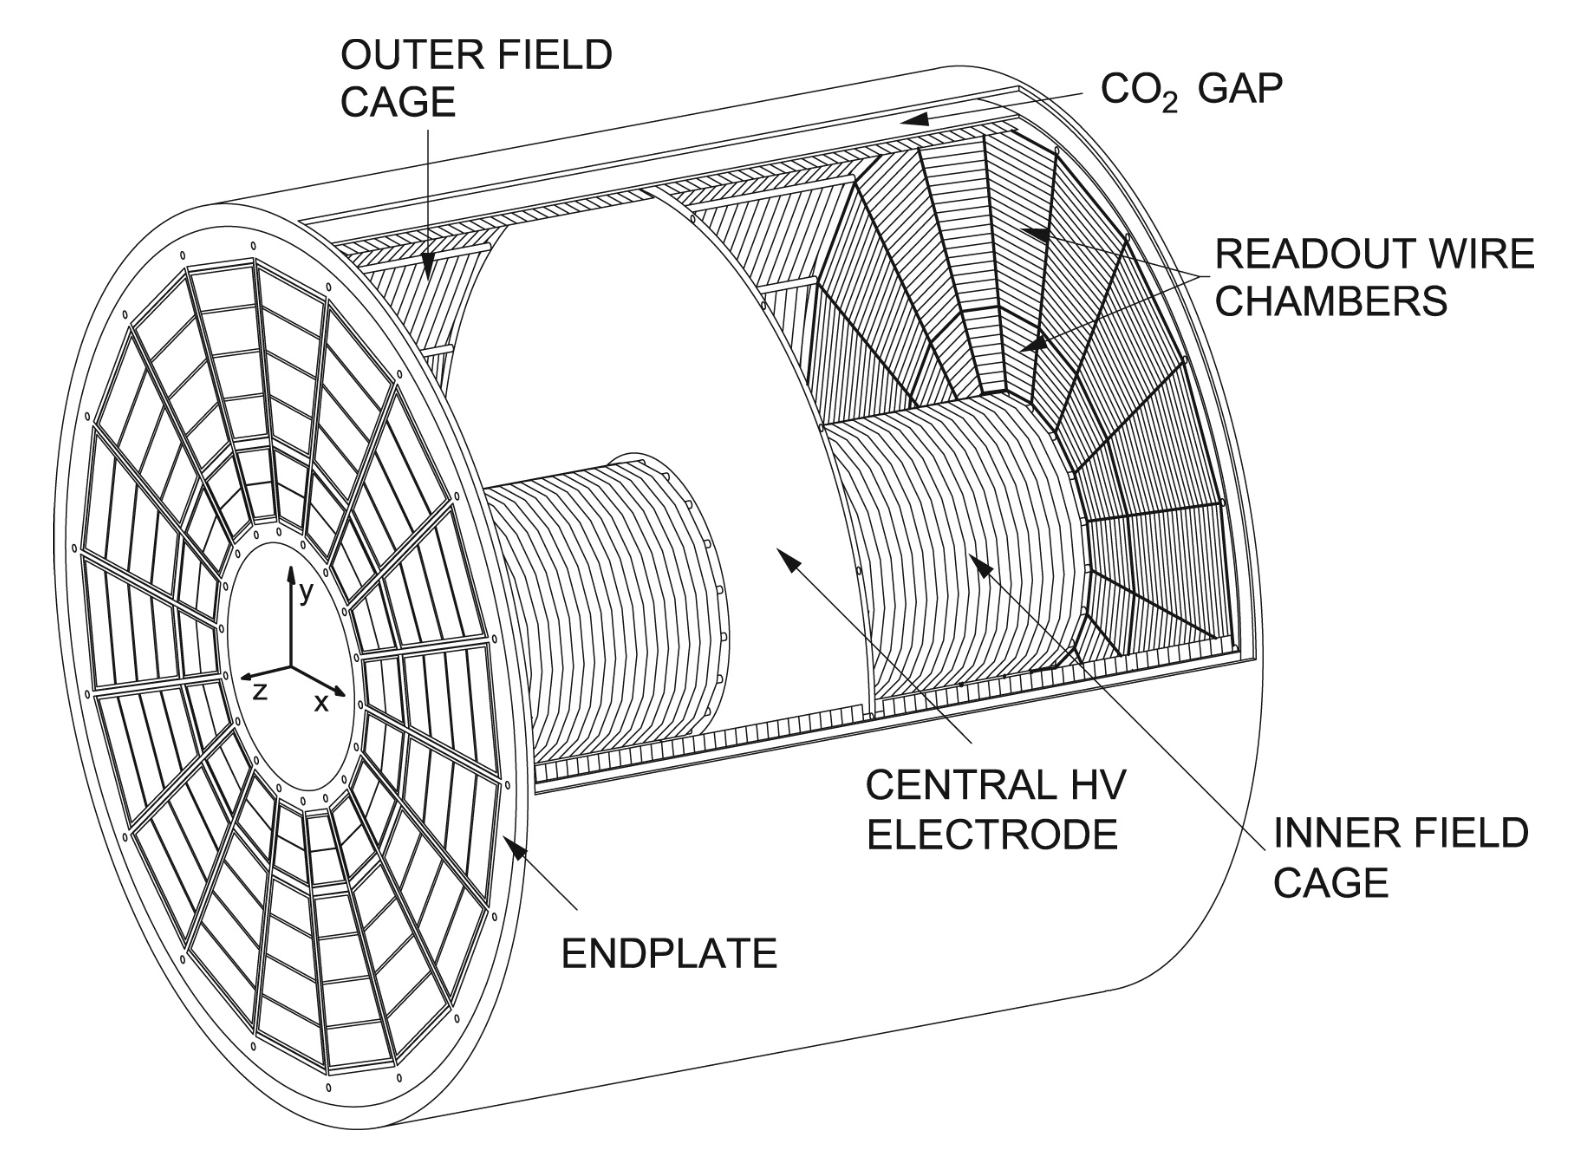
\includegraphics[width=0.7\linewidth]{Images/ND-GAr/alice_tpc}
	\caption[Diagram of the ALICE TPC, showing the two drift chambers, inner and outer field cages and readout chambers.]{Diagram of the ALICE TPC, showing the two drift chambers, inner and outer field cages and readout chambers. Figure taken from Ref. \cite{DUNE2021NDCDR}.}
	\label{fig:alice_tpc}
\end{figure}

It will use a 90:10 molar fraction $\mathrm{Ar}$:$\mathrm{CH}_{4}$ mixture at $10~\mathrm{bar}$. With this baseline gas mixture light collection is not possible, as the quenching gas absorbs most of the VUV photons. Additional R\&D efforts are underway, to understand if different mixtures allow for the light signal to be used to provide a $t_{0}$ while maintaining stable charge gain.

\subsubsection{ECal}

\begin{figure}[t]
	\centering
	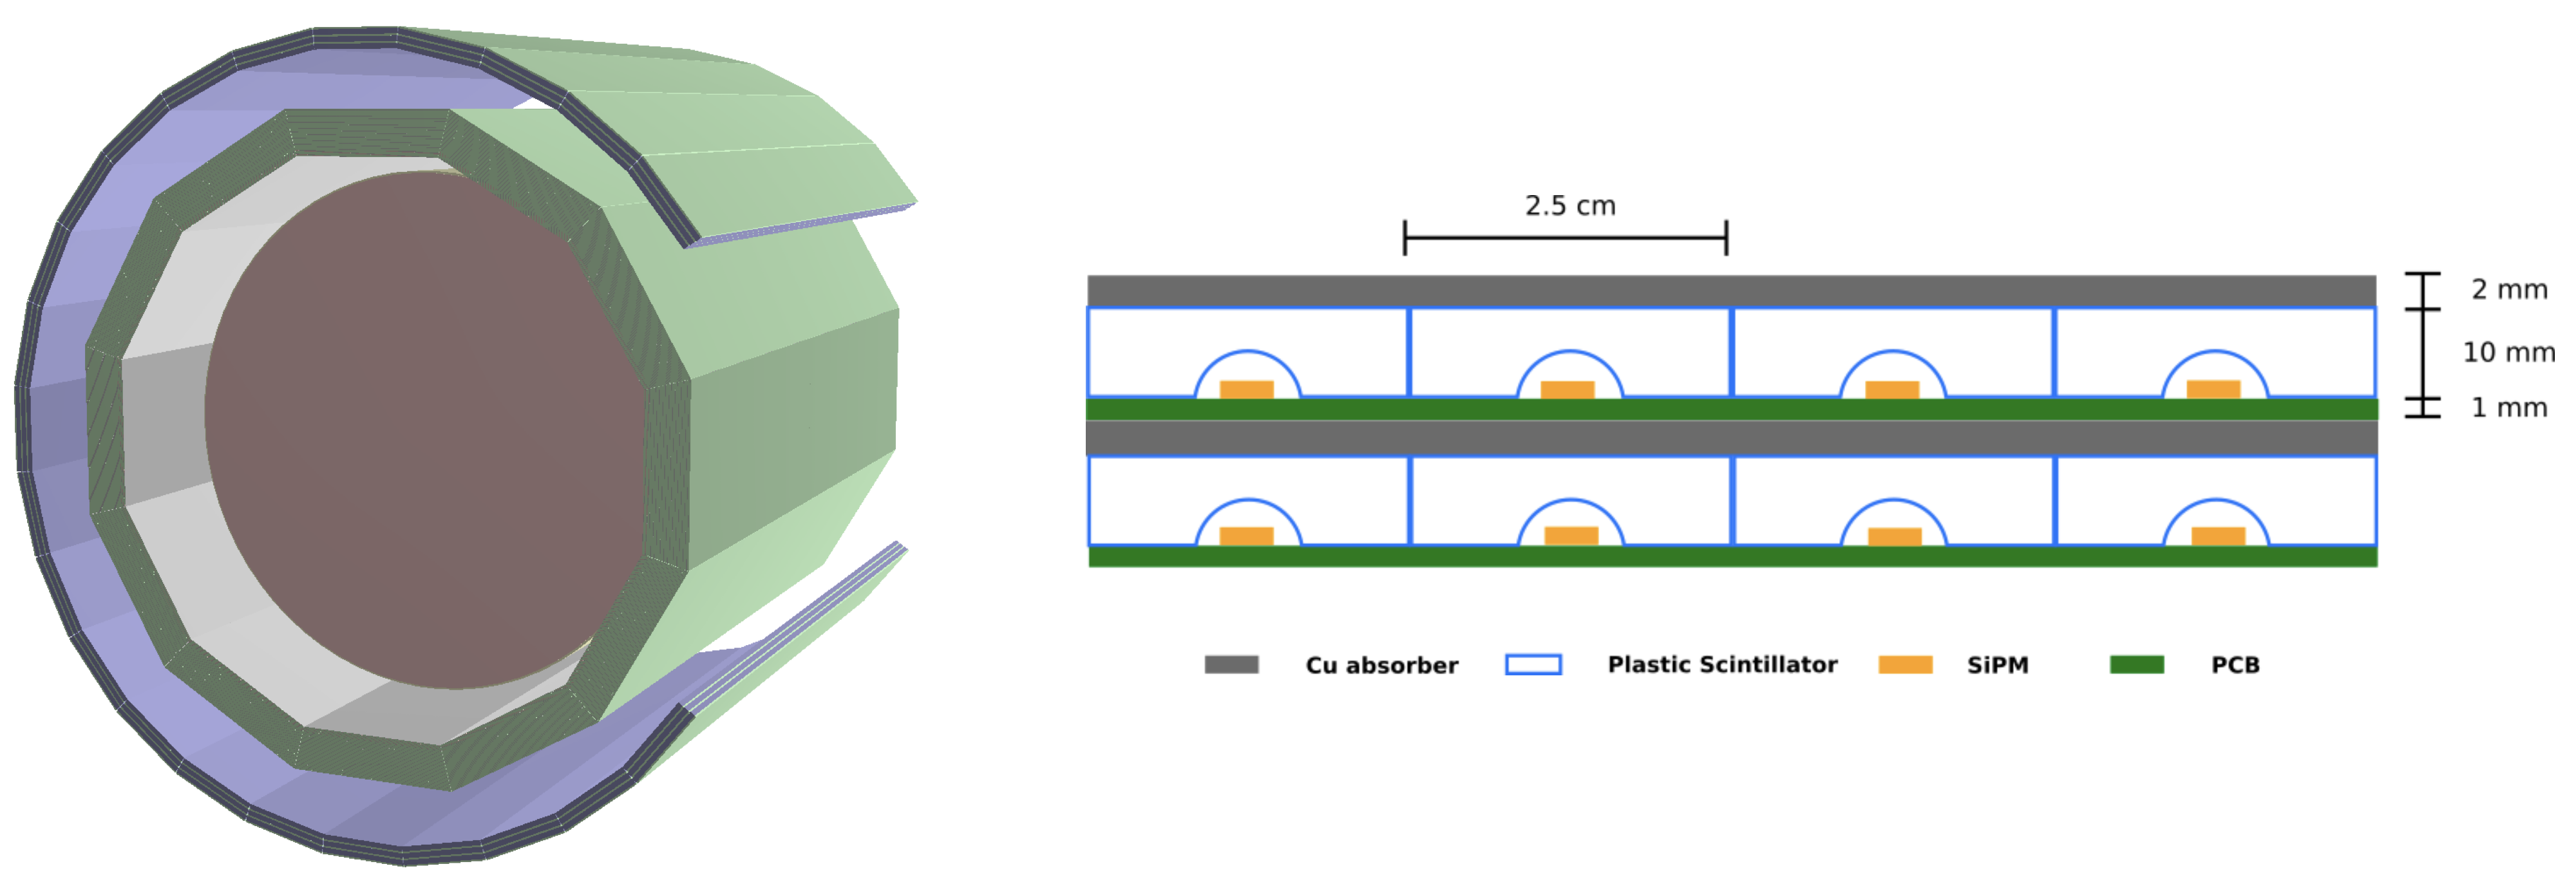
\includegraphics[width=0.99\linewidth]{Images/ND-GAr/ndgar_ecal}
	\caption[Diagram of the ALICE TPC, showing the two drift chambers, inner and outer field cages and readout chambers.]{View of the 12-sided ECal barrel and outer muon tagger geometries (left) and layout of the ECal tile layers for the $2~\mathrm{mm}$ Cu, $10~\mathrm{mm}$ scintillator option (right). Figure adapted from Ref. \cite{DUNE2021NDCDR}.}
	\label{fig:ndgar_ecal}
\end{figure}

The main role of the ND-GAr ECal is the calorimetric measurement of the electron energies and the reconstruction of photons, in particular those from neutral pion decays. Also, the ECal is able to provide a $t_{0}$ timestamp for neutrino interactions, by associating its activity to the tracks in the HPgTPC. The ECal will also be able to perform neutron reconstruction using time-of-flight measurements, and reject external backgrounds thanks to its sub-nanosecond time resolution.

The ECal design features three independent subdetectors, two end caps at each side and a barrel surrounding the HPgTPC. Each of the detectors is divided in modules, which combine alternating layers of plastic scintillator and absorber material readout by SiPMs. The inner scintillator layers consist of $2.5\times2.5~\mathrm{cm}^{2}$ high-granularity tiles, whereas the outer layers are made out of $4~\mathrm{cm}$ wide cross-strips spanning the whole module length. The current barrel geometry consists of 8 tile layers and 34 strip layers, while the end caps feature 6 and 36 respectively. The thickness of the scintillator layers is $7~\mathrm{mm}$, and $5~\mathrm{mm}$ for the Pb absorber layers. The 12-sided geometry of the ECal barrel (left) and the layout of the tile layers (left) can be seen in Fig. \ref{fig:ndgar_ecal}.

\subsubsection{Magnet}

The ND-GAr magnet design, known as the Solenoid with Partial Yoke (SPY), consists of two coupled solenoids with an iron return yoke \cite{DUNESPY2023}. The idea behind the design is to have a solenoid as thin as possible, as well as a return yoke mass distribution that minimises the material budget between ND-LAr and ND-GAr. The magnet needs to provide a $0.5~\mathrm{T}$ field in the direction perpendicular to the beam, parallel to the drift electric field. It needs to host the pressure vessel and the surrounding ECal, which points to a inner diameter of $\sim6.4~\mathrm{m}$.

The solenoid is a single layer coil, based on niobium titanium superconducting Rutherford cable. The total length of the coil is $7.5~\mathrm{m}$. The bobbin will be split in four segments, grouped in pairs with two identical cryostats connected in series. The iron yoke features an aperture in the upstream side, to minimise the energy loss of the muons coming from ND-LAr. Still, its material will be enough to reduce the magnetic field reaching SAND, and also stop the charged pions produced inside the HPgTPC.

\subsubsection{Muon system}

The design of the ND-GAr muon system is still in a preliminary stage. Its role is to distinguish between muons and pions punching through the ECal. This is especially important for wrong-sign determination, to separate these from neutral current events.

In its current form, the muon system consists of three layers of longitudinal sampling structures. It alternates $10~\mathrm{cm}$ Fe absorber slabs with $2~\mathrm{cm}$ plastic scintillator strips. The transverse granularity required is still under study.

\subsection{R\&D efforts}

\begin{figure}[t]
	\centering
	\includegraphics[width=0.99\linewidth]{Images/ND-GAr/toad.png}
	\caption[Photographs of the TOAD pressure vessel at RHUL.]{Photographs of the TOAD pressure vessel at RHUL. The TPC is mounted inside the vessel, and the OROC is supported by an aluminium frame. Figure taken from Ref. \cite{Ritchie-Yates2023}.}
	\label{fig:toad}
\end{figure}

There are several ND-GAr-related prototypes, mostly focused on the TPC charge readout and electronics. The priority is to test the full readout chain, in a high-pressure environment, using a gas mixture with high argon fraction. A detailed summary of these can be found in the DUNE Phase II white paper \cite{DUNE2024Phase2}.

\subsubsection{Multi-Wire Proportional Chambers}

As mentioned before, the original ND-GAr design repurposes the MWPCs of the ALICE TPC, which became available after the recent upgrade \cite{ALICETPC2020}. These were operated using a 90:10:5 $\mathrm{Ne}$:$\mathrm{CO}_{2}$:$\mathrm{N}_{2}$ gas mixture at $1~\mathrm{atm}$. Therefore, their performance needed to be studied in an argon gas environment at high pressure.

The Gas-argon Operation of ALICE TPC (GOAT) test stand tested the ALICE readout chambers at high pressure. In particular, it used one of the previously operated ALICE inner MWPCs, also known as IROCs, in a pressure vessel rated to $10~\mathrm{atm}$. It measured the gas gain at various pressure points, voltages and gas mixtures.

The Test stand of an Overpressure Argon Detector (TOAD) tested an ALICE outer MWPC, also known as OROC, up to $5~\mathrm{atm}$. During its time at RHUL, it was used to study the achievable gas gain of the OROC \cite{Ritchie-Yates2023}. At the moment, it is being commissioned at Fermilab for a full detector test of the readout electronics and the DAQ.

Figure \ref{fig:toad} shows the interior of the TOAD pressure vessel. The TPC is mounted inside the vessel on three rails. The back of the OROC, supported by an aluminium frame, can be seen at the front.

\begin{figure}[h!]
	\begin{subfigure}{0.49\textwidth}
		\centering
		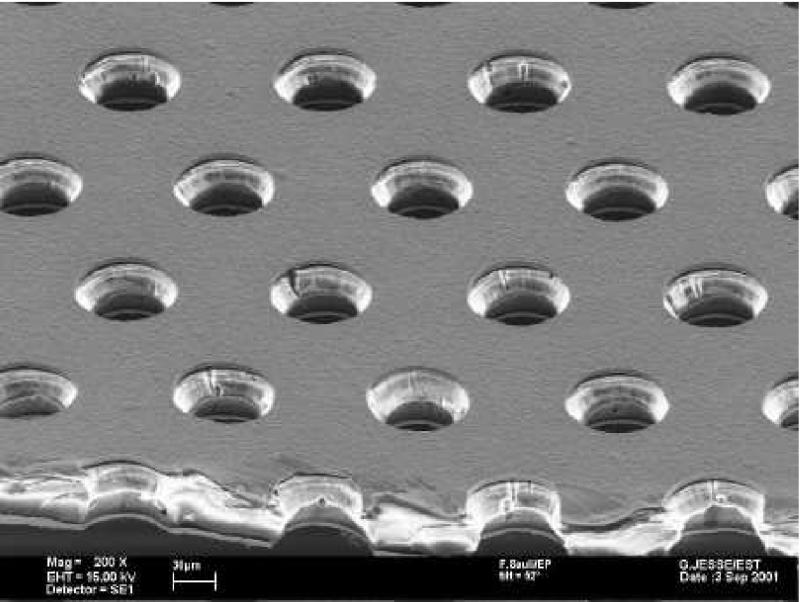
\includegraphics[width=.90\linewidth]{Images/ND-GAr/GEM_photo.jpg}
	\end{subfigure}
	\begin{subfigure}{0.49\textwidth}
		\centering
		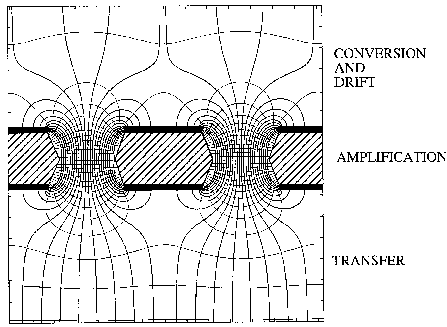
\includegraphics[width=.90\linewidth]{Images//ND-GAr/GEM_diagram.pdf}
	\end{subfigure}
	\caption[Electron microscope image and schematic diagram of a GEM electrode.]{Left panel: electron microscope image of a $50~\mu\mathrm{m}$ thick GEM electrode, with hole pitch and diameter of $140$ and $70~\mu\mathrm{m}$, respectively. Right panel: Schematics of a GEM electrode cross section, showing the electric field lines around the holes. Figures taken from Ref. \cite{Sauli2016}.}
	\label{fig:gem}
\end{figure}

\subsubsection{Gas Electron Multiplier}

An alternative to the MWPC option is the use of GEMs. These are a type of micro-pattern detector, where the ionisation electrons passing through the holes in the GEM layers are accelerated by a high-intensity electric field. The acceleration causes the electrons to ionise the medium, resulting in an avalanche which increases the signal exponentially \cite{Sauli1997}. GEMs are used in numerous experiments that need a high spatial resolution, like ALICE \cite{Lippmann2016} and CMS \cite{Calabria2016} after their upgrades.

Figure \ref{fig:gem} (left panel) shows an electron microscope picture of a $50~\mu\mathrm{m}$ thick GEM electrode, with a pitch between neighbouring holes of $140~\mu\mathrm{m}$ and a hole diameter of $70~\mu\mathrm{m}$. A schematic representation of the cross section of a GEM layer is shown in Fig. \ref{fig:gem} (left panel).

The Gaseous Argon T0 (GAT0\footnote{Spanish for cat.}) prototype studies the use of thick GEMs made out of glass to achieve optical imaging of the primary ionisation. Using a $10~\mathrm{atm}$ pressure vessel, the goal is to study different argon-based mixtures that allow for a precise $t_{0}$ determination.

The GEM Over-pressurized with Reference Gases (GORG\footnote{Persian for wolf.}) test stand is currently testing a GEM-based charge readout, using a triple-GEM stack.

\section{Far Detector}

\begin{figure}[t]
	\centering
	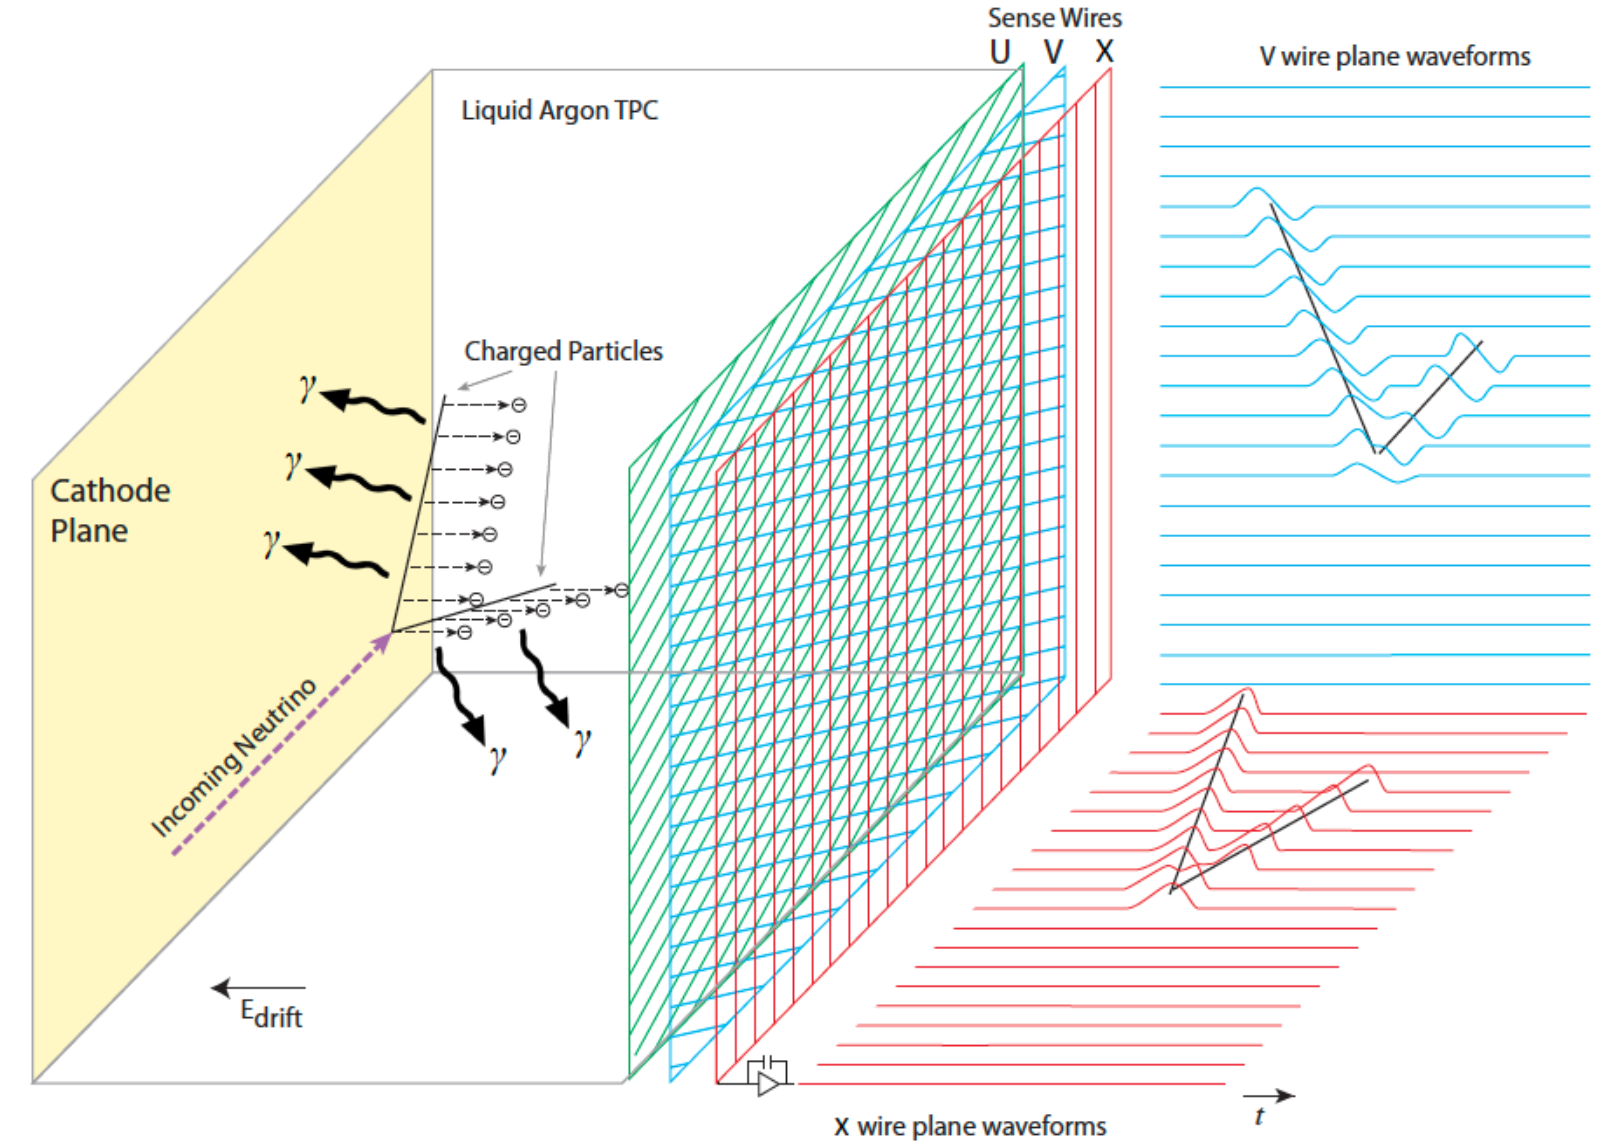
\includegraphics[width=0.8\linewidth]{Images/DUNE/FD/tpc}
	\caption[Schematic diagram showing the operating principle of a LArTPC with wire readout.]{Schematic diagram showing the operating principle of a LArTPC with wire readout. Figure taken from Ref. \cite{DUNE2020TDR1}.}
	\label{fig:lartpc}
\end{figure}

The DUNE FD complex will sit $1300~\mathrm{km}$ away from the beam target and $1.5~\mathrm{km}$ underground at SURF, South Dakota. Two caverns will host the four FD modules, two of them per cavern, each embedded in cryostats of dimensions $18.9~\mathrm{m} ~ (\text{w}) \times 17.8~\mathrm{m} ~ (\text{h}) \times 65.8~\mathrm{m} ~ (\text{l})$. A central, smaller cavern will host the cryogenic system.

Three out of the four modules are confirmed to be LArTPC detectors, with a LAr fiducial mass of at least $10 ~ \mathrm{kt}$ each. The first and third FD modules, FD-1 and FD-3, will use a Vertical Drift (VD) technology, whereas the second module, FD-2, will have a Horizontal Drift (HD) direction. The technology for the fourth module is still to be decided. Detailed descriptions of the HD and VD designs can be found in the DUNE FD TDR Volume IV \cite{DUNE2020TDR4} and the DUNE FD VD TDR \cite{DUNEVDTDR}, respectively.

For each event, with energies ranging from a few $\mathrm{MeV}$ to several $\mathrm{GeV}$, these detectors collect both the scintillation light and the ionisation electrons created when the charged particles produced in the neutrino-nucleus interactions ionise the argon nuclei. In both HD and VD designs the characteristic $128~\mathrm{nm}$ scintillation light of argon is collected by a photon detection system (PDS). This light will indicate the time at which electrons start to drift, thus enabling reconstruction over the drift coordinate when compared to the time when the first ionisation electrons arrive to the anode. Reconstruction of the topology in the transverse direction is achieved using the charge readout. Fig. \ref{fig:lartpc} illustrates the detection principle described, for the case of a HD detector with a wire readout.

\subsection{Horizontal Drift}

\begin{figure}[t]
	\centering
	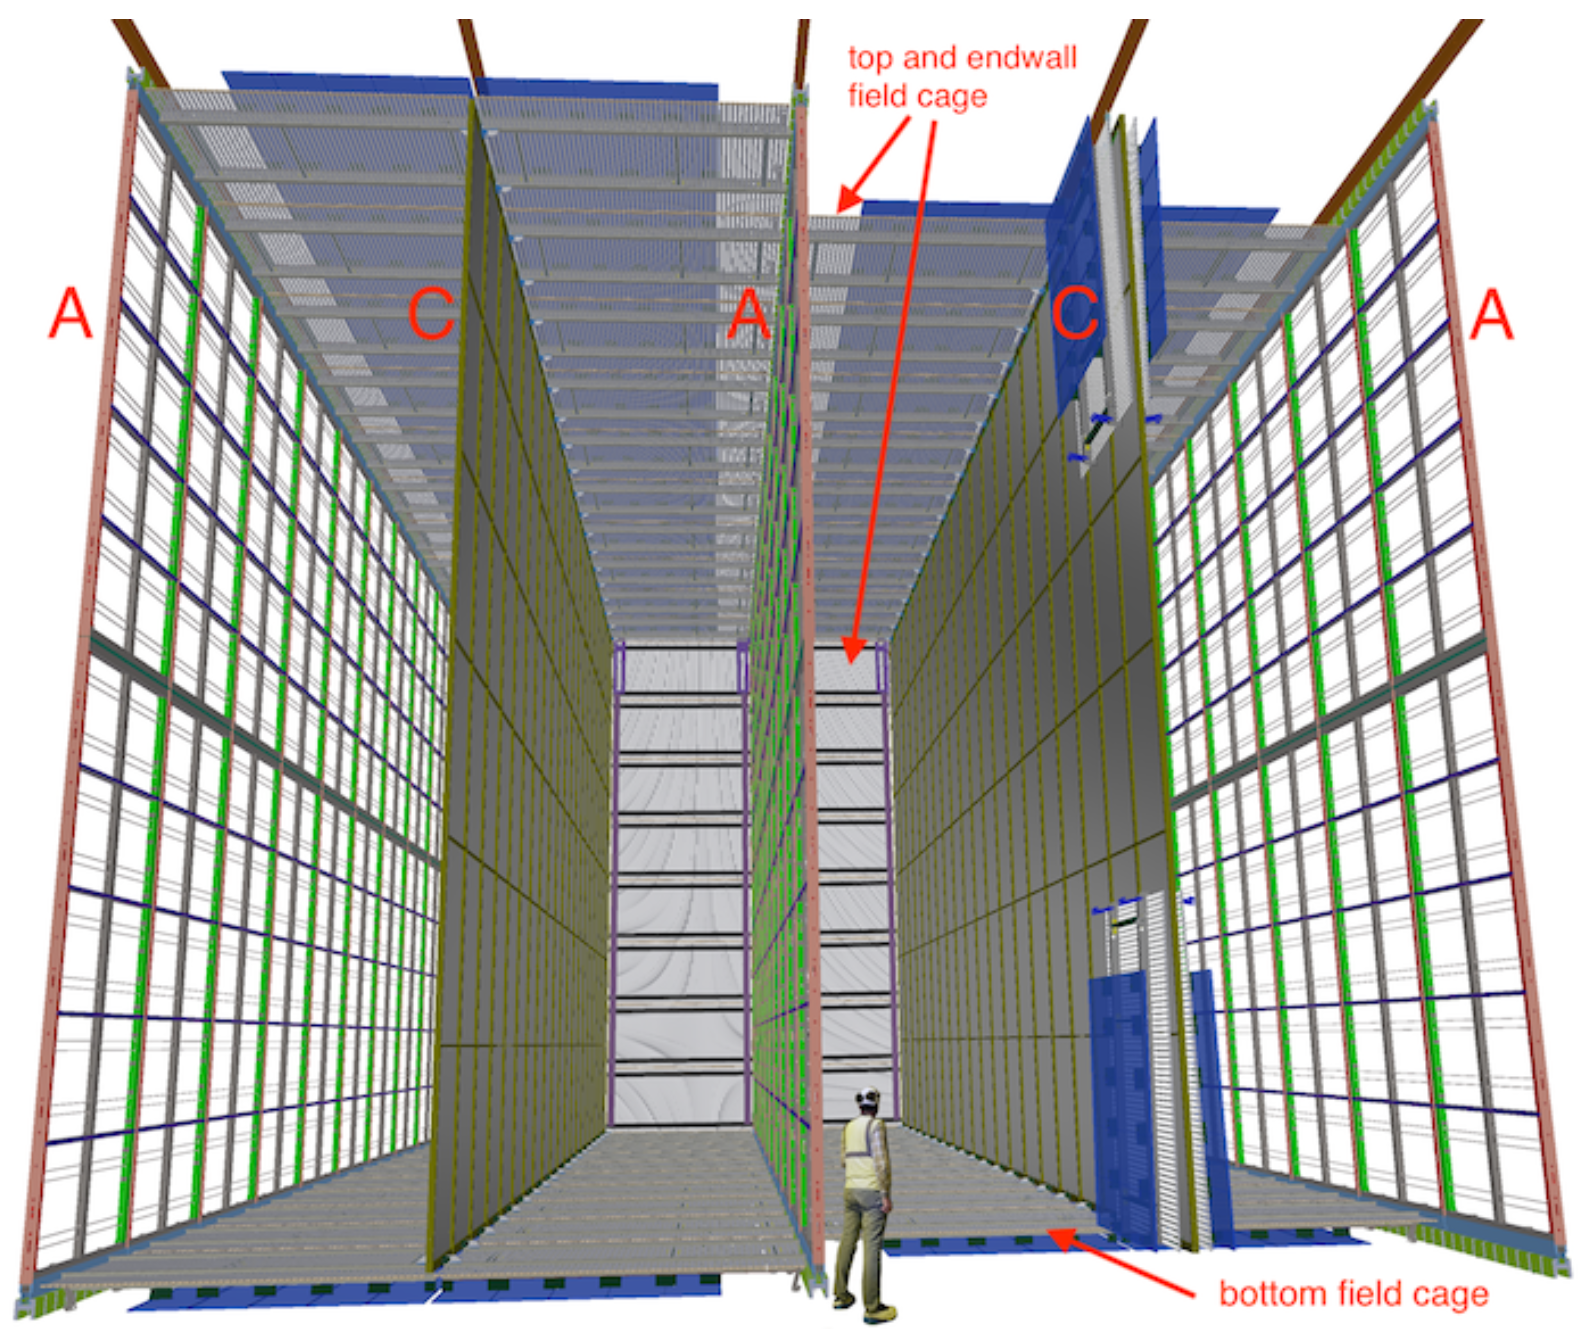
\includegraphics[width=0.65\linewidth]{Images/DUNE/FD/dune_hd}
	\caption[Proposed design for the FD-2 module following the HD principle.]{Proposed design for the FD-2 module following the HD principle. Figure taken from Ref. \cite{DUNE2020TDR1}.}
	\label{fig:dune_hd}
\end{figure}

In the HD design the ionisation electrons produced as charged particles traverse the LAr drift horizontally towards the anode planes, due to the effect of an electric field. These anode planes are made out of three layers of wire readout. This design, previously known as single-phase (SP), was tested in the ProtoDUNE-SP detector at CERN. The prototype collected data from a hadron beam and cosmic rays, providing high-quality data sets for calibration and performance studies.

Each FD HD detector module is divided in four drift regions, with a maximum drift length of $3.5~\mathrm{m}$, by alternating anode and cathode walls. The surrounding field cage ensures the uniformity of the $500~\mathrm{V/cm}$ horizontal electric field across the drift volumes. The three anode walls, which constitute the charge readout of the detector, are built by stacking anode plane assemblies (APAs), 2 high times 25 wide. The design of the HD modules is shown in Fig. \ref{fig:dune_hd}.

Each APA is made of 2560 active wires arranged in three layers, plus an extra grid layer, wrapped around a metal frame. The two induction wire planes, U and V, sit at $\pm 35.7^{\circ}$ to the vertical on each side of the APA. The collection and shielding plane wires, X and G, run parallel to the vertical direction. The ionisation electrons drift past the induction planes, generating bipolar signals on those wires, and are collected by the collection plane, producing a monopolar positive signal. The spacing between the wires is $\sim 5~\mathrm{mm}$, and it defines the spatial resolution of the APA.

\begin{figure}[t]
	\centering
	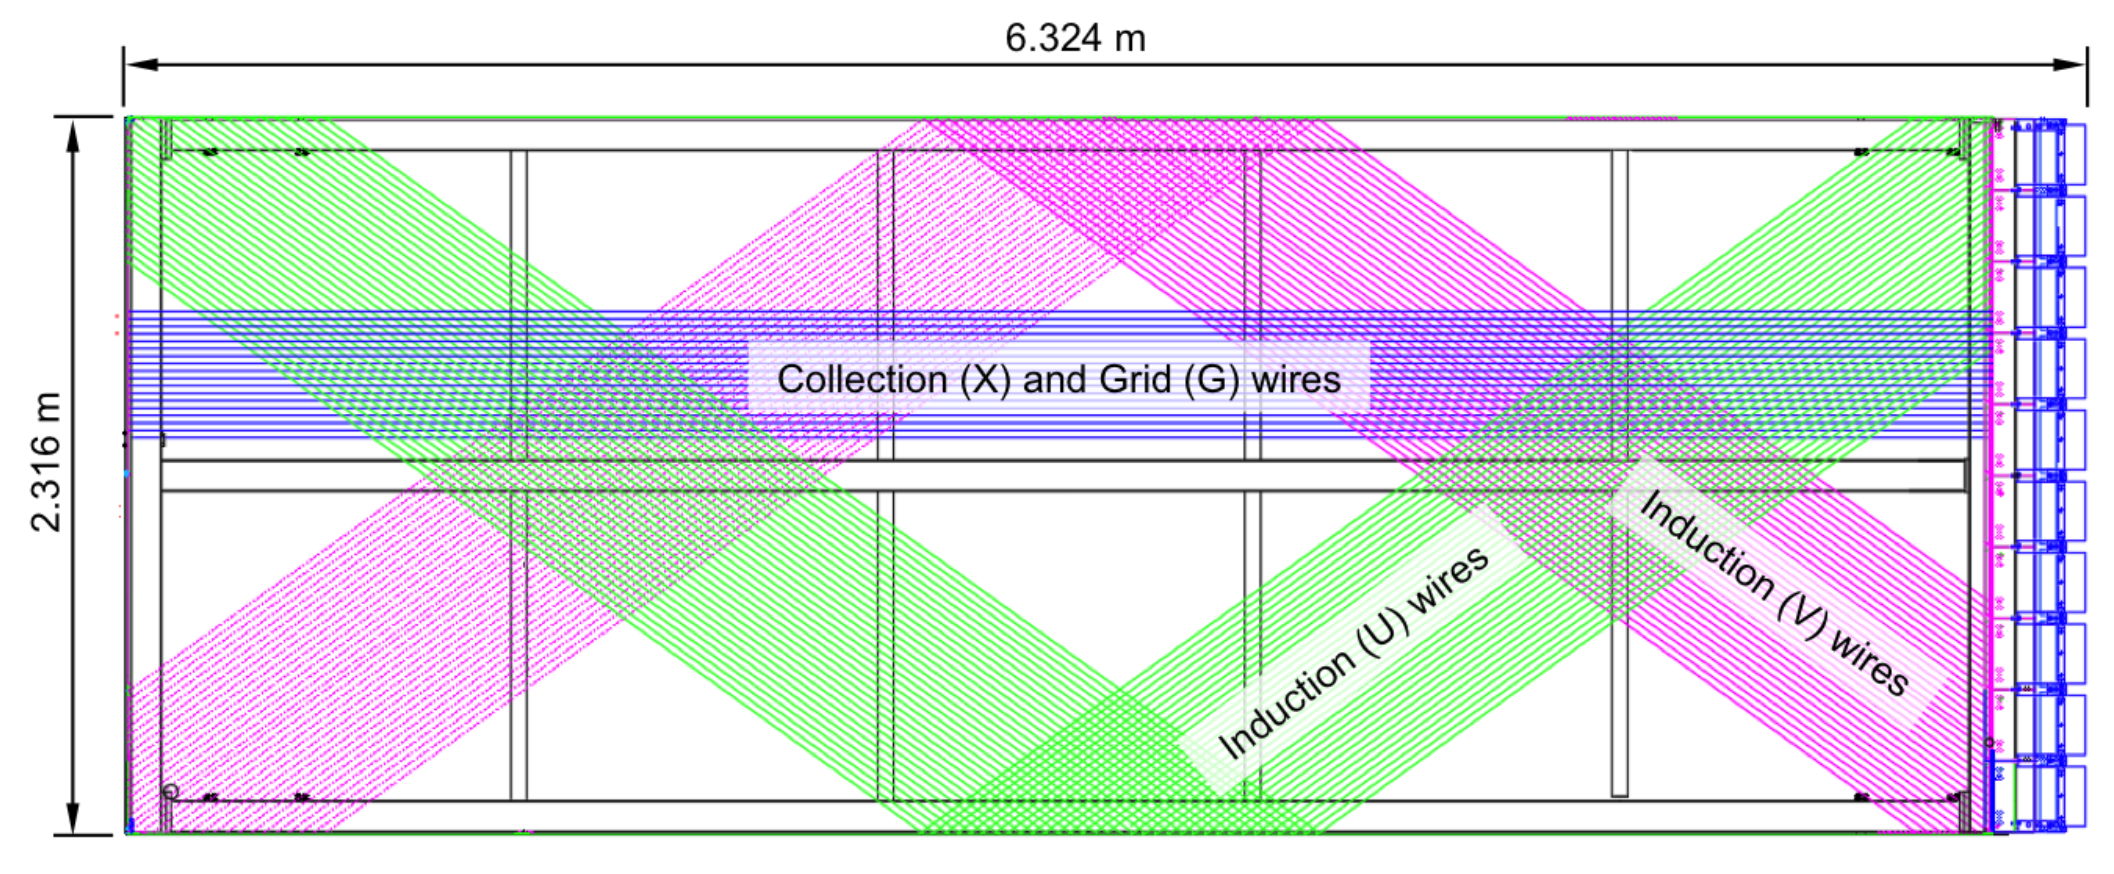
\includegraphics[width=1\linewidth]{Images/DUNE/FD/APA_wires}
	\caption[Schematic representation of an APA frames showing the U, V, X and G wires.]{Schematic representation of an APA. The black lines represent the APA steel frame. The green and magenta lines correspond to the direction of the U and V induction wires respectively. The blue lines indicate the direction of the X collection wires and the wire shielding G. Figure taken from Ref. \cite{DUNE2020TDR1}.}
	\label{fig:apa}
\end{figure}

The front-end readout electronics, or cold electronics as they are immerse in the LAr, are attached to the top of the up APAs and the bottom of the down APAs. Mounted on the front-end mother boards we have a series of ASICs that digitise the signals from the collection and induction planes. Each wire signal goes to a charge-sensitive amplifier, then to a pulse-shaping circuit, and finally to the analogue-to-digital converter. This part of the process happens inside the LAr to minimise the number of cables penetrating the cryostat. The digitised signals come out finally via a series of high-speed serial links to the warm interface boards (WIBs), from where the data is sent to the back-end DAQ through optical fibers.

\begin{figure}[t]
	\begin{subfigure}{0.49\textwidth}
		\centering
		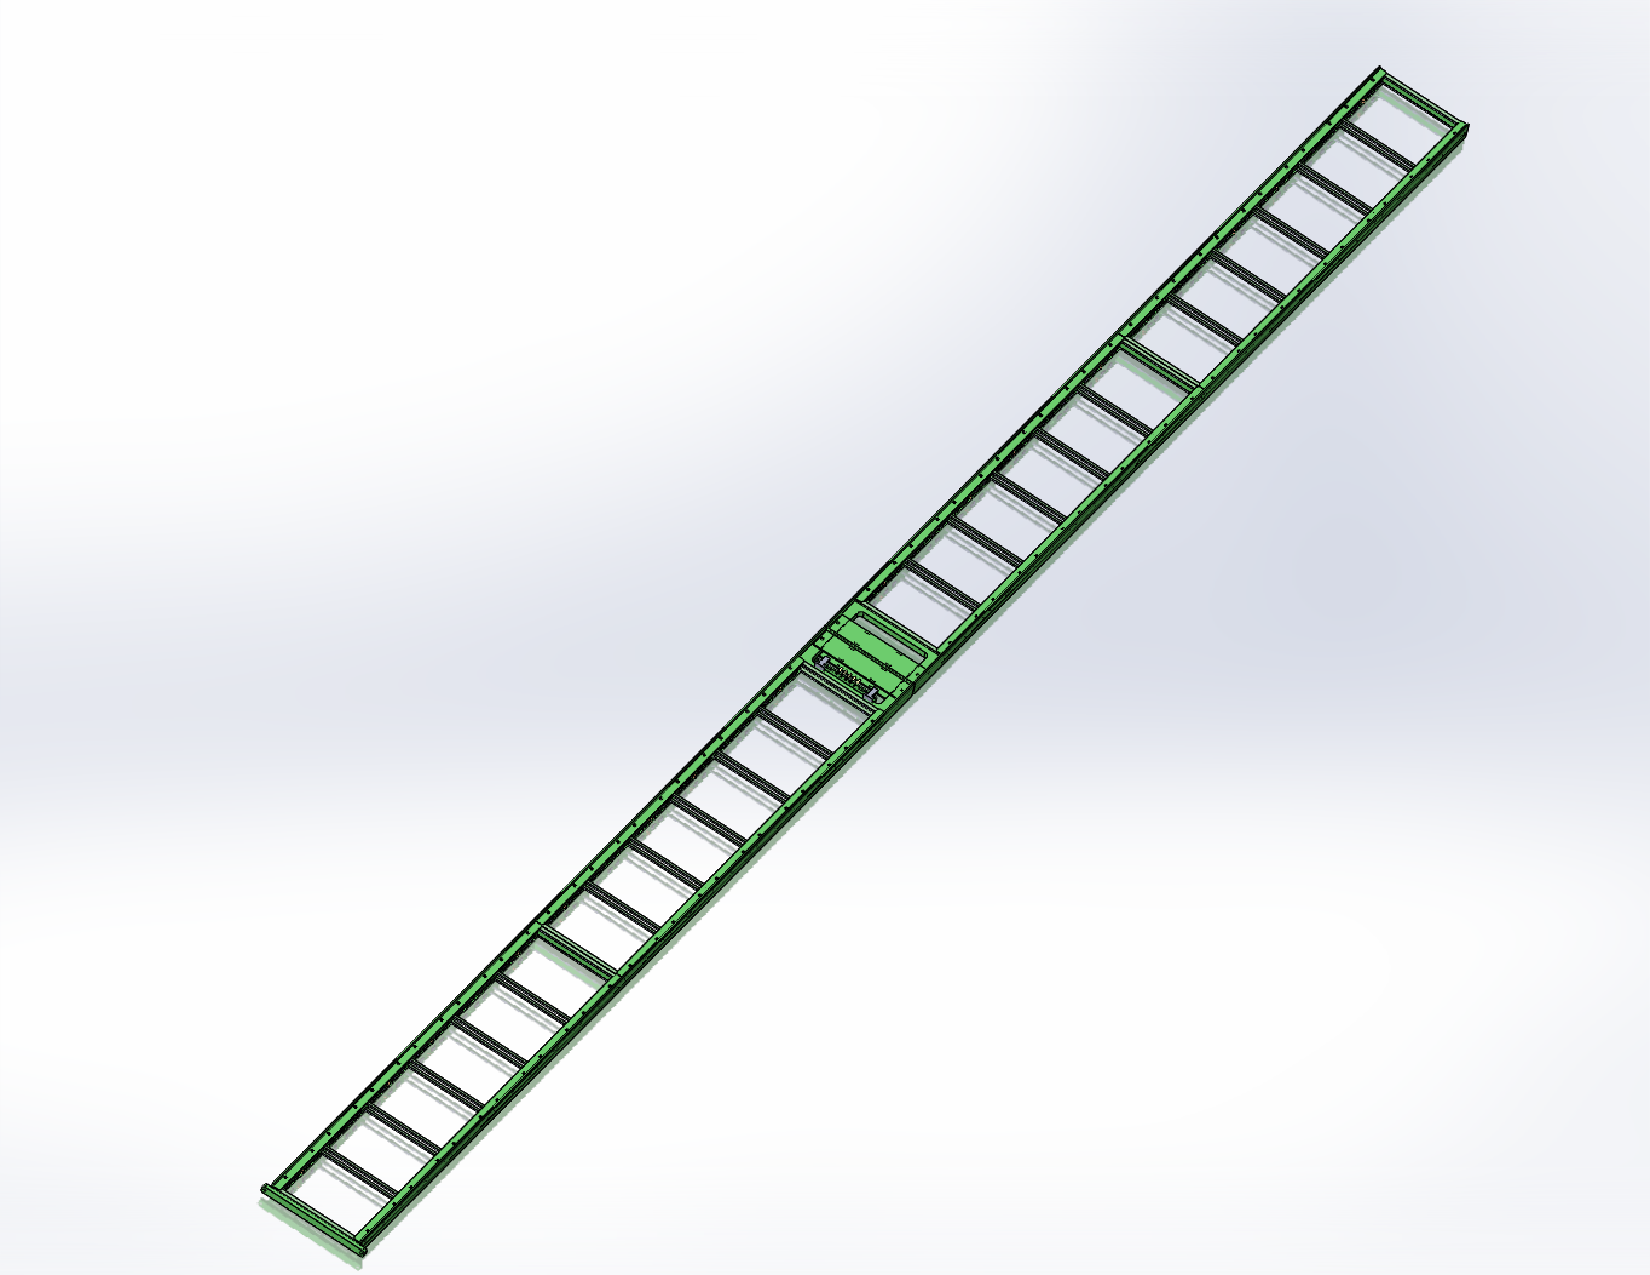
\includegraphics[width=.90\linewidth]{Images/DUNE/FD/pds-module}
	\end{subfigure}
	\begin{subfigure}{0.49\textwidth}
		\centering
		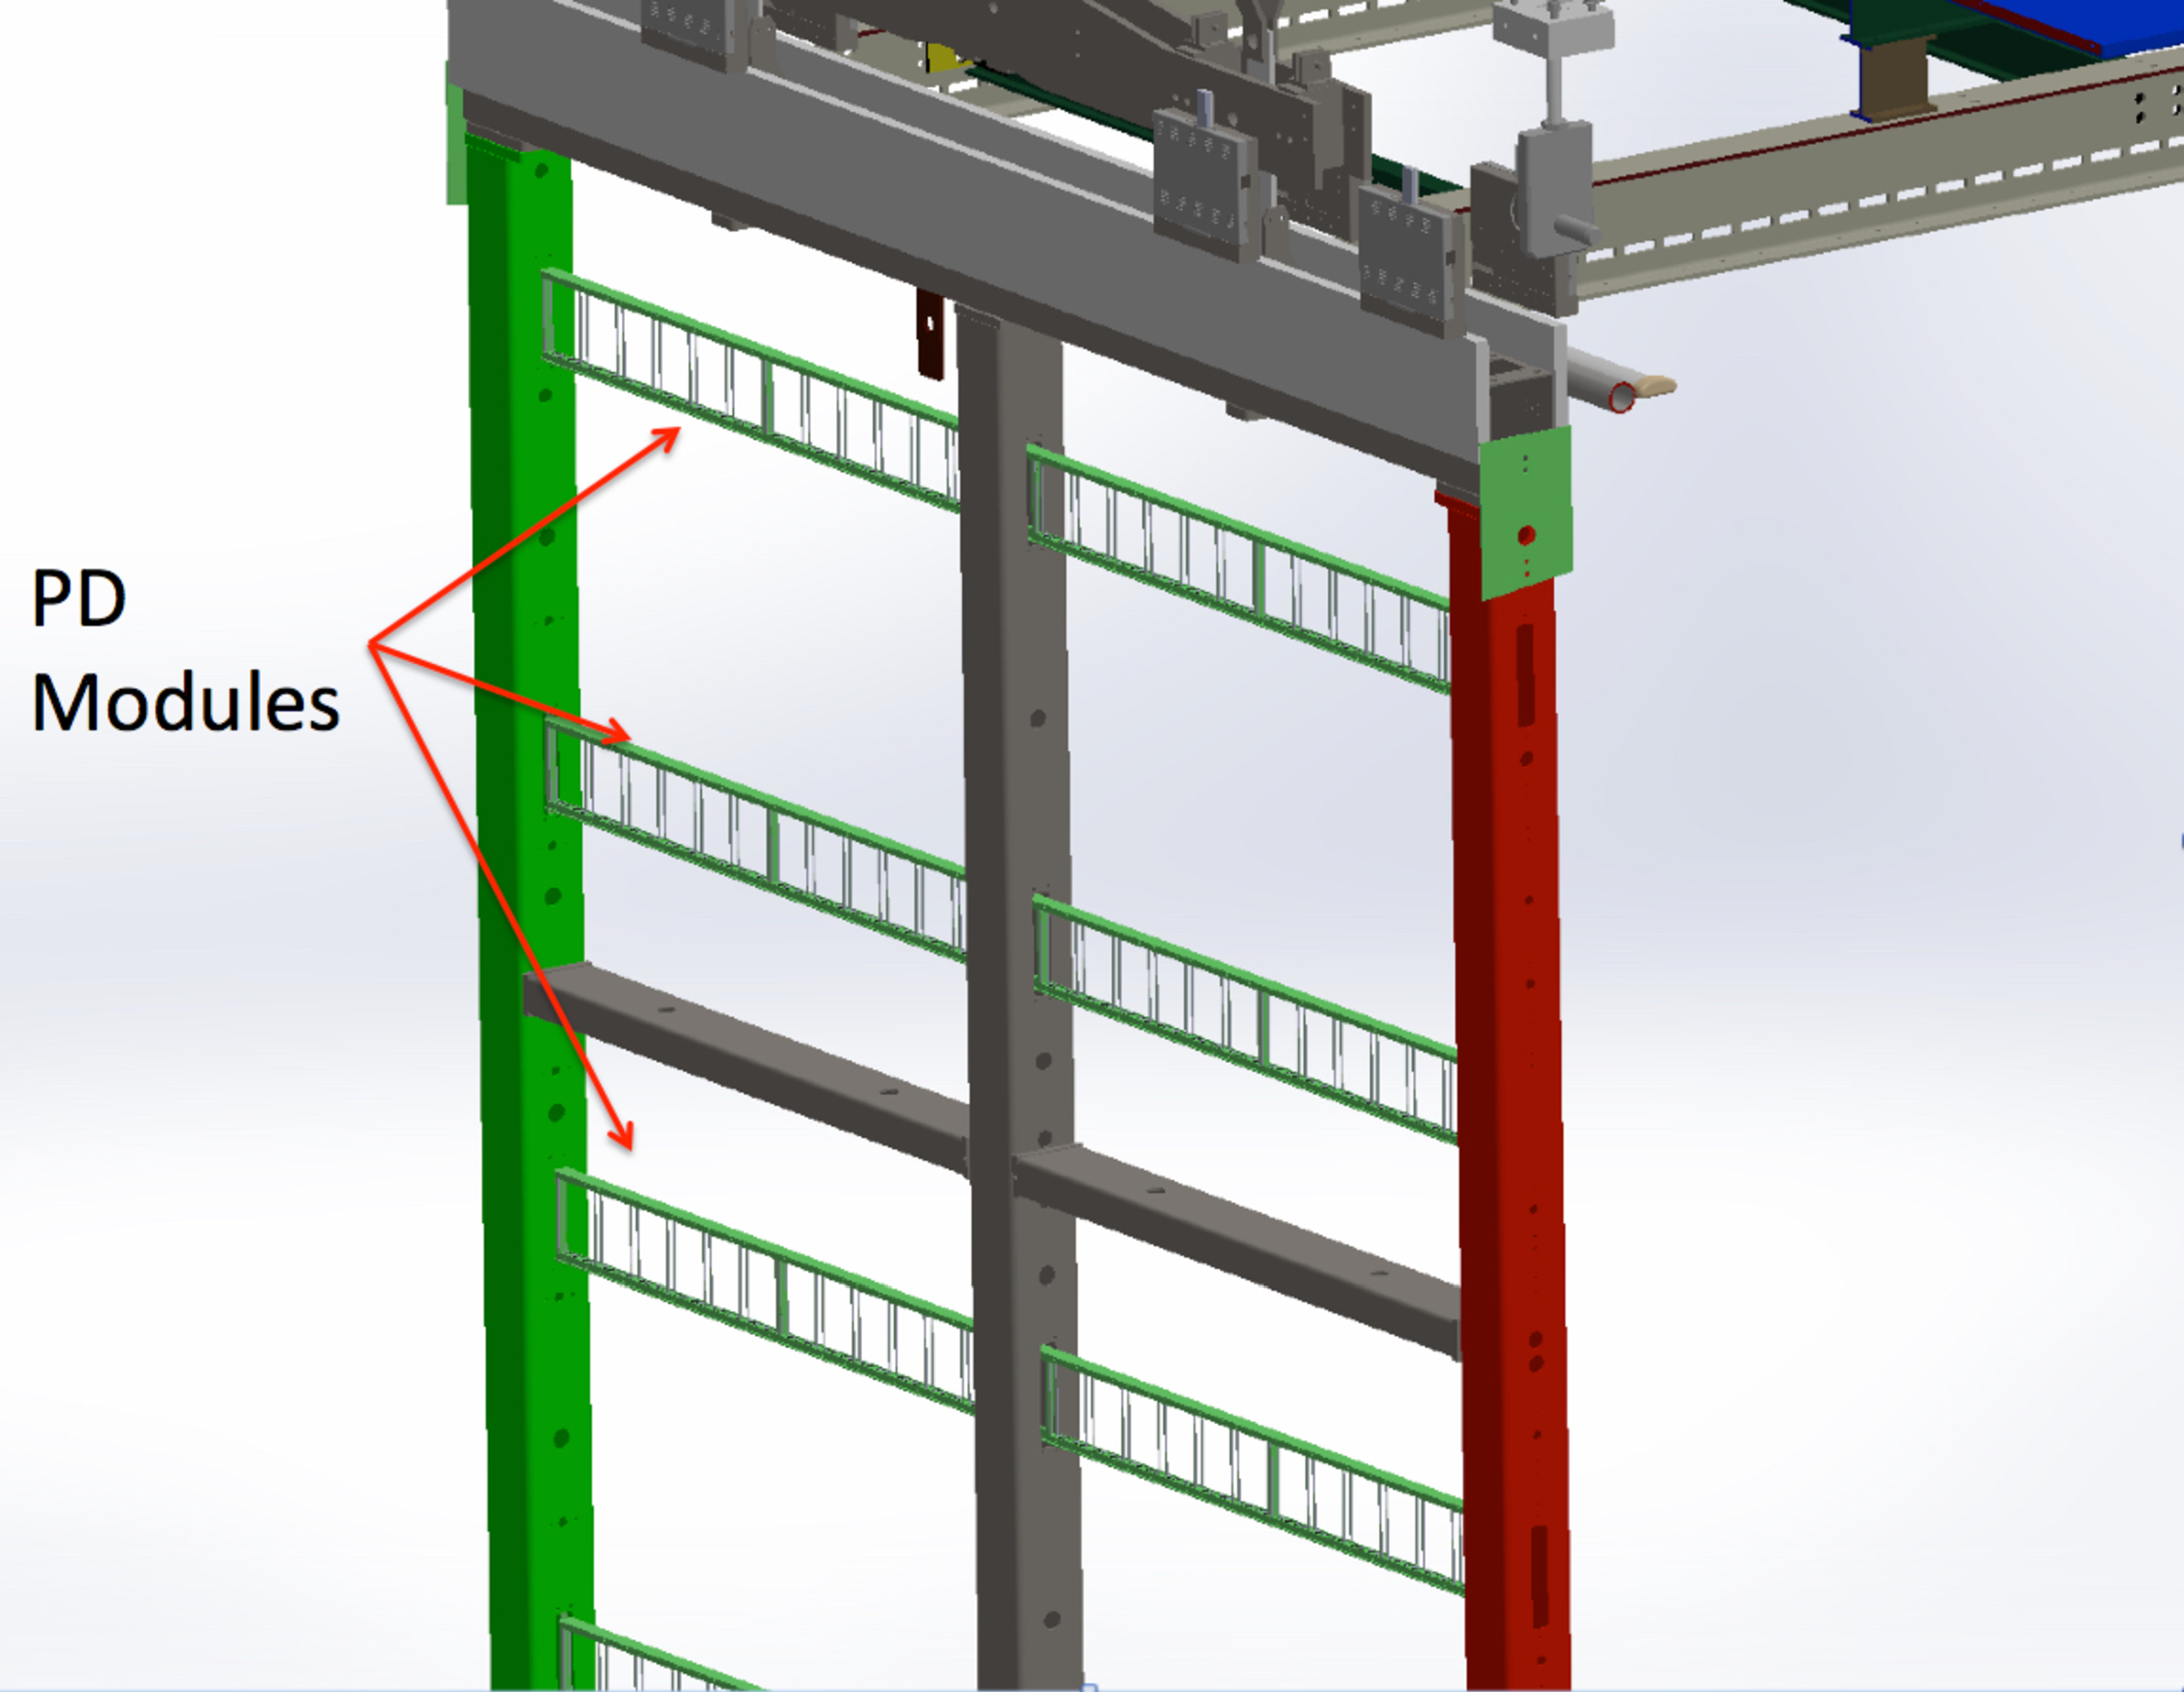
\includegraphics[width=.90\linewidth]{Images/DUNE/FD/pds-in-apa-assembly}
	\end{subfigure}
	\caption[A PDS module containing 24 X-ARAPUCAs and the location of the modules on the APA frames.]{A PDS module containing 24 X-ARAPUCAs (left) and the location of the modules on the APA frames (right). Figure taken from Ref. \cite{DUNE2020TDR1}.}
	\label{fig:dune_pds}
\end{figure}

The PDS uses modules of X-ARAPUCA devices, mounted on the APA frames between the wire planes. Each X-ARAPUCA consists of layers of dichroic filter and wavelength-shifter. They shift the VUV scintillation light into the visible spectrum, sending then the visible photons to silicon photomultiplier (SiPM) devices. The PDS modules are $209~\mathrm{cm}\times12~\mathrm{cm}\times2~\mathrm{cm}$ bars, containing 24 X-ARAPUCAs. There are 10 of these PDS modules per APA. Fig. \ref{fig:dune_pds} shows a PDS module (left) and the placement of the modules on the APAs (right).

\begin{comment}
	When using a SP LArTPC there is no electron amplification, thus low noise is required by CE to extract the signals from the wires with a minimum S/N. In the worst operating case (short drift electron lifetime $\tau = 3 \ \mathrm{ms}$ and $E_{drift} = 250 \ \mathrm{V/cm}$) at least $10^{4}$ electrons will arrive to the anode from a minimum ionizing particle (MIP) near the cathode (farthest possible distance). Requiring at most $10^{3}$ electrons of equivalent noise charge (ENC) we will have a S/N $~\sim10$ for the collection wires. In the induction wires it results in S/N $\sim 5$, because of the bipolar shape of the signal. Keeping noise low (improving S/N) is crucial to achieve the physics goals. It allows proper event reconstruction and expand the boundaries on low-energy phenomena (SNB, $^{39}$Ar calibrations, etc.). Noise also affect DAQ bandwidth, and can be a problem for astrophysical measurements.
\end{comment}

\subsection{Vertical Drift}

\begin{figure}[t]
	\centering
	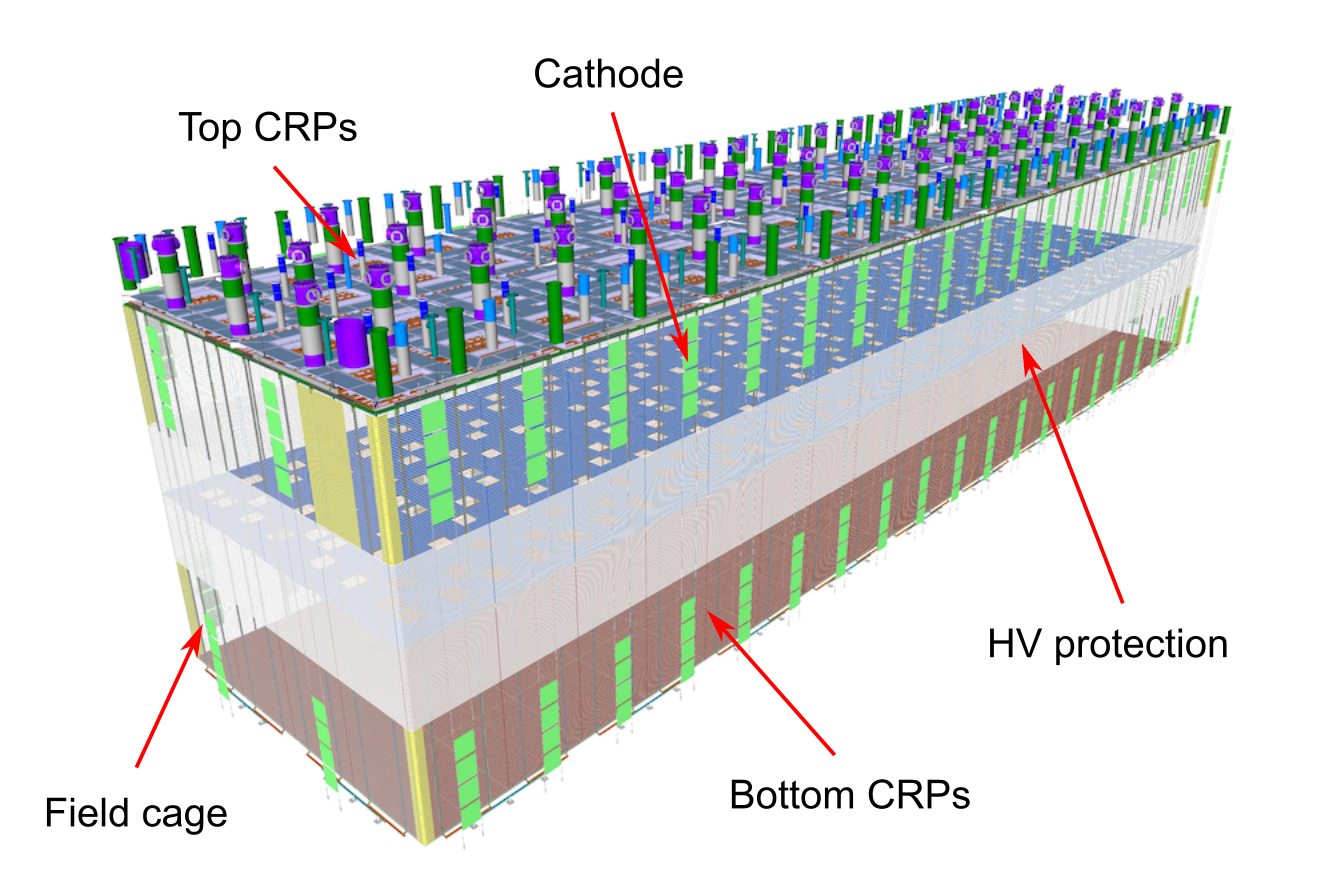
\includegraphics[width=0.70\linewidth]{Images/DUNE/FD/dune_vd}
	\caption[Proposed design for the FD-1 and FD-3 modules following the VD principle.]{Proposed design for the FD-1 and FD-3 modules following the VD principle. Figure adapted from Ref. \cite{DUNEVDTDR}.}
	\label{fig:dune_vd}
\end{figure}

In the VD case the ionisation electrons will drift vertically until they meet a printed circuit board-based (PCB) readout plane. It is based on the original dual-phase (DP) design deployed at CERN, in the detector known as ProtoDUNE-DP, which used a vertical drift design with an additional amplification of the ionisation electrons using a GAr layer above the liquid phase. The VD module incorporates the positive features of the DP design without the complications of having the LAr-GAr interface.

The current design of the FD VD module consists of two drift chambers with a maximum drift distance of $6.5~\mathrm{m}$. A cathode plane splits the detector volume perpendicular to the drift direction, while the two anode planes are connected to the bottom and top walls of the detector. The layout of a VD module is shown in Fig. \ref{fig:dune_vd}. Compared with the HD design, the VD option offers a slightly larger instrumented volume and a more cost-effective solution for the charge readout.

\begin{figure}[t]
	\centering
	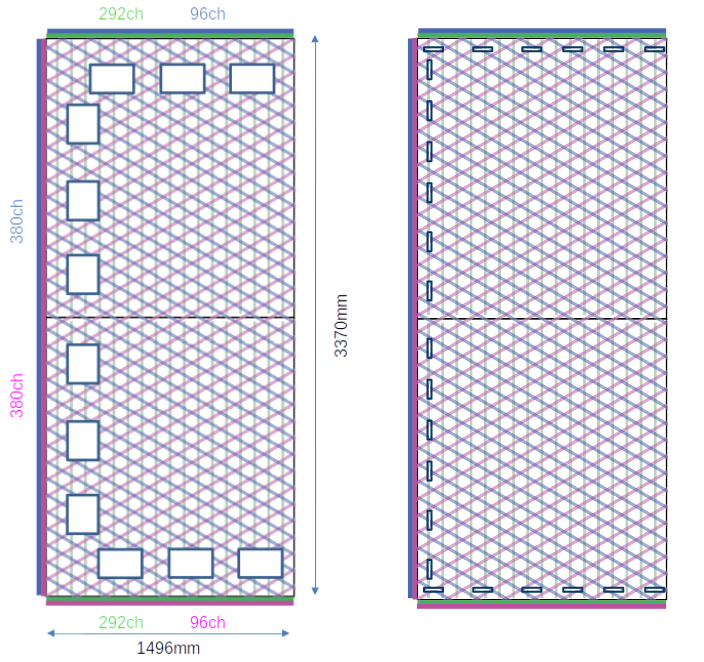
\includegraphics[width=0.70\linewidth]{Images/DUNE/FD/3V_anode_layout}
	\caption[Schematic representation of the electrode strip configuration for a top and bottom CRU.]{Schematic representation of the electrode strip configuration for a top (left) and bottom (right) CRU. Figure taken from Ref. \cite{DUNEVDTDR}.}
	\label{fig:dune_cru}
\end{figure}

As in the HD design, each drift volume features a $500~\mathrm{V/cm}$ electric field and a field cage that ensures its uniformity. The anode planes are arrays of $3.4~\mathrm{m}\times3~\mathrm{m}$ charge-readout planes (CRPs). These are formed by a pair of charge-readout units (CRUs), which are built from two double-sided perforated PCBs, with their perforations aligned. The perforations allow the drift electrons to pass between the layers.

The PCB face opposite to the cathode has a copper guard plane which acts as shielding, while its reverse face is etched with electrode strips forming the first induction plane. The outer PCB has electrode strips on both faces, the ones facing the inner PCB form the second induction plane, while the outermost ones form the collection plane. Fig. \ref{fig:dune_cru} shows the layout of the electrode strips for the top (left) and bottom (right) CRUs. The magenta and blue lines represent the first and second induction planes, respectively, and the green lines correspond to the collection plane.

The PDS in the VD module will use the same X-ARAPUCA technology developed for the HD design. The plan is to place the PDS modules on the cryostat walls and on the cathode, in order to maximise the photon yield.

%\subsection{Module of opportunity}

\begin{figure}[t]
	\centering
	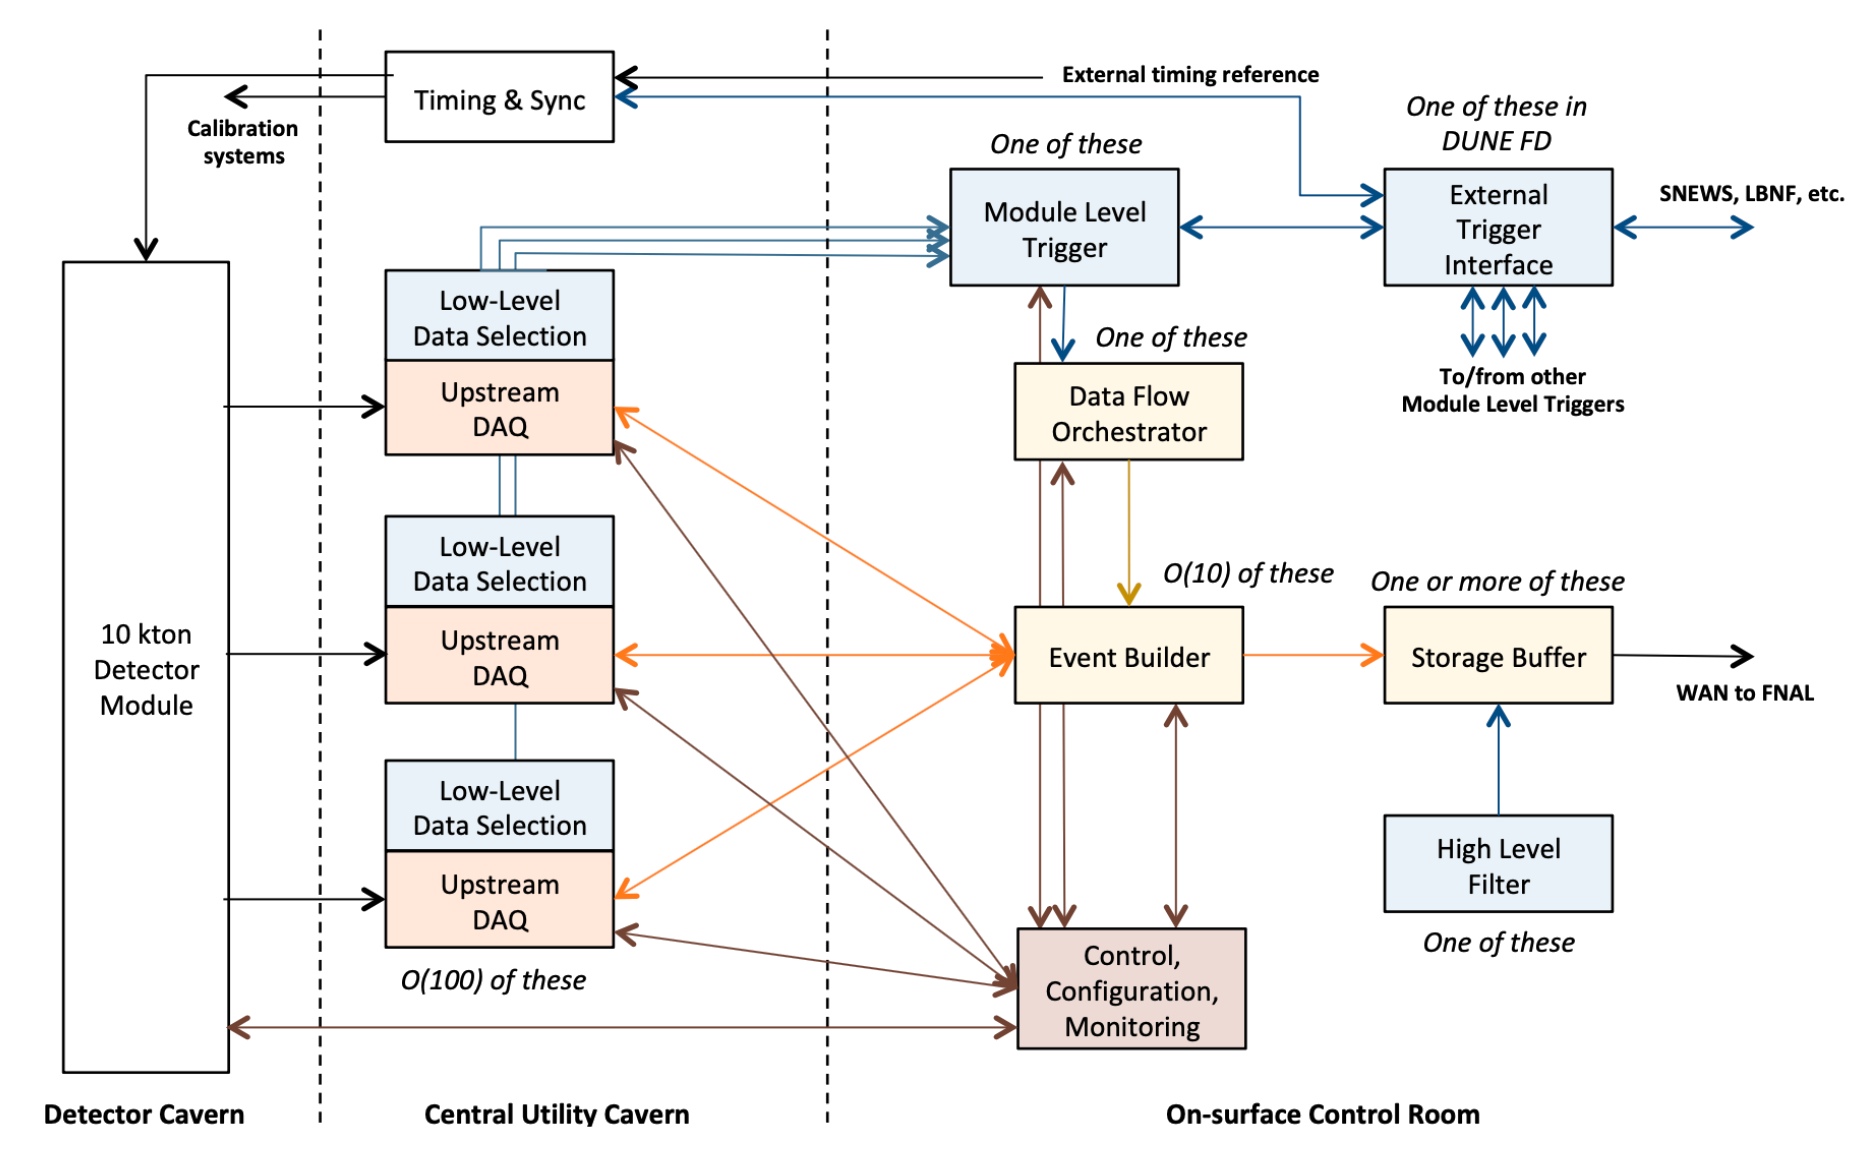
\includegraphics[width=0.8\linewidth]{Images/DUNE/FD/DAQ_detailed2}
	\caption[Detailed diagram of the DUNE FD DAQ system.]{Detailed diagram of the DUNE FD DAQ system. Figure taken from Ref. \cite{DUNE2020TDR4}.}
	\label{fig:daq1}
\end{figure}

\subsection{FD Data Acquisition System}

The data acquisition (DAQ) system receives, processes and stores data from the detector modules. In the case of DUNE, the DAQ architecture is designed to work for all FD modules interchangeably, except some aspects of the upstream part which may depend on the specific module technology.

The enormous sample rate and the number of channels in the TPC and PDS readouts will produce a very large volume of data. These pose really strong requirements and challenges to the DUNE FD DAQ architecture. It will be required to read out data of the order of ten thousand or more channels at rates of a few MHz. To cope with the huge data volume, segmented readouts and compression algorithms are used to reduce the data rate to manageable levels.

The DAQ system of the DUNE FD is composed of five different subsystems. The first one is the upstream DAQ, which receives the raw data from the detector, buffers it and performs some low-level pre-processing. The minimally processed data is then fed into a hierarchical data selection system, which then performs a module level trigger decision. In case of a positive decision, a trigger command is produced and executed by the data flow orchestrator, located in the back-end (BE) DAQ subsystem. Subsequently, the DAQ BE retrieves the relevant data from the buffers located in the upstream DAQ, adds all the data into a cohesive record, and saves it to permanent storage. Watching over all the other subsystems we also have the control, configuration and monitoring subsystem and the time and synchronization subsystem. Figure \ref{fig:daq1} shows a schematic diagram of the DAQ system, showing the different subsystems and their relations.

A notorious challenge for the DUNE DAQ system comes from its broad physics goals. We must be prepared to process events spanning a wide range of time windows, from $5 \ \mathrm{ms}$ in the case of beam and cosmic neutrinos and nucleon decay events, to $100 \ \mathrm{s}$ in the case of SNBs. This requires a continuous readout of the detector modules. Moreover, because of the off-beam measurements, we need to ensure the capabilities of online data processing and self-triggering. Having this into account, together with the technical constraints, the DUNE FD DAQ faces a series of challenges: it needs to be fault tolerant and redundant to reduce downtime, accommodate new components while it keeps serving the operational modules, have large upstream buffers to handle SNB physics, be able to support a wide range of readout windows, and reduce the throughput of data to permanent storage to be at most $30 \ \mathrm{PB/year}$.
%\chapter{ND-GAr}
\label{chapter:nd_gar}

ND-GAr is a magnetised, high-pressure gaseous argon TPC (HPgTPC), surrounded by an electromagnetic calorimeter (ECal) and a muon detector (commonly refer to as $\mu$ID). A detailed discussion on the requirements, design, performance and physics of ND-GAr can be found in the DUNE ND CDR \cite{DUNE2021NDCDR} and the ND-GAr whitepaper (cite).

In DUNE Phase II ND-GAr will fulfill the role of TMS, measuring the momentum and sign of the charged particles exiting ND-LAr. Additionally, it will be able to measure neutrino interactions inside the HPgTPC, achieving lower energy thresholds than those of the ND and FD LArTPCs. By doing so ND-GAr will allow to constrain the relevant systematic uncertainties for the LBL analysis even further.

The goal of the present chapter is to review the requirements that the physics program of DUNE impose on ND-GAr, present the current status of its design and describe the GArSoft package, its simulation and reconstruction software.

\section{Requirements}

The primary requirement for ND-GAr is to the measure the momentum and charge of muons from $\nu_{\mu}$ and $\bar{\nu}_{\mu}$ CC interactions in ND-LAr, in order to measure their energy spectrum. To achieve the sensitivity to the neutrino oscillation parameters described in the DUNE FD TDR Volume II \cite{DUNE2020TDR2} ND-GAr should be able to constrain the muon energy within a $1\%$ uncertainty or better. The main constraint will come from the calibration of the magnetic field, performed using neutral kaon decays in the HPgTPC.

Another requirement for ND-GAr is the precise measurement of neutrino interactions on argon for the energies relevant to the neutrino oscillation program. The goal is to constrain the cross section systematic uncertainties in the regions of phase space that are not accessible to ND-LAr. This requires the kinematic acceptance for muons in ND-GAr to exceed that of ND-LAr, being comparable to the one observed in the FD.

ND-GAr should also be able to the relationship between true and reconstructed energy from neutrino interactions on argon with low thresholds, being sensitive to particles that are not observed or may be misidentified in ND-LAr. In particular, ND-GAr needs to have low tracking thresholds in order to measure the spectrum of pions and protons produced in final-state interactions (FSI). It also must be able to accurately measure the pion multiplicity in 1, 2 and 3 pions final states, to inform the pion mass correction in the LArTPCs.

\section{Reference design}

The final design of ND-GAr is still under preparation. However, a preliminary baseline design was in place at the time of the ND CDR. This section summarises the main features of that design, as it is also the one used for the default geometry in our simulation. A DUNE Phase II whitepaper, discussing the different options under consideration for the ND-GAr design, is in progress. 

\subsection{HPgTPC}

The reference design for the ND-GAr HPgTPC follow closely that of the ALICE TPC. It is a cylinder with a central high-voltage cathode, generating the electric field for the two drift volumes, with a maximum drift distance of $2.5~\mathrm{m}$ each. The anodes will be instrumented with charge readout chambers. The original design repurposed the multi-wire proportional readout chambers of ALICE, however the current R\&D efforts focus on a gas electron multiplier option instead. Fig. \ref{fig:alice_tpc} shows a schematic diagram of the ALICE TPC design. The basic ND-GAr geometry will resemble this, except for the inner field cage.

\begin{figure}[t]
	\centering
	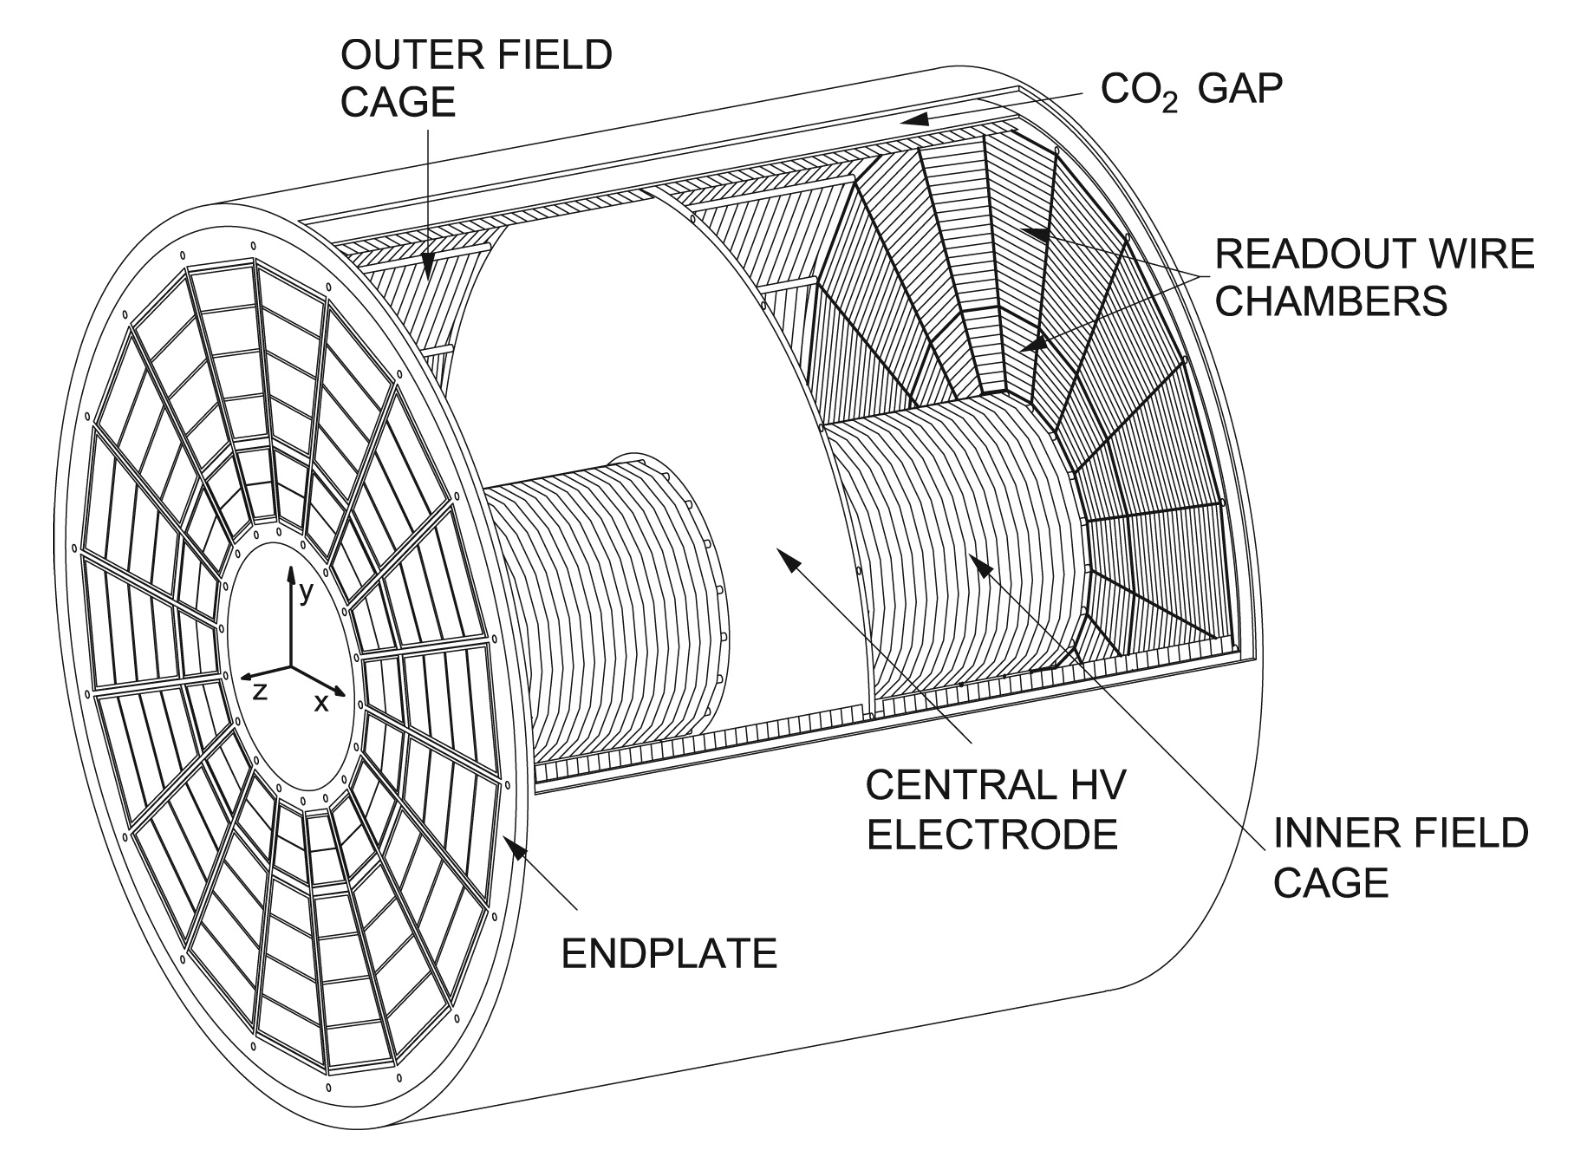
\includegraphics[width=0.7\linewidth]{Images/ND-GAr/alice_tpc}
	\caption[Diagram of the ALICE TPC, showing the two drift chambers, inner and outer field cages and readout chambers.]{Diagram of the ALICE TPC, showing the two drift chambers, inner and outer field cages and readout chambers. Figure taken from Ref. \cite{DUNE2020TDR1}.}
	\label{fig:alice_tpc}
\end{figure}

It will use a 90-10 molar fraction argon-CH$_{4}$ mixture at $10~\mathrm{bar}$. With this baseline gas mixture light collection is not possible, as the quenching gas absorbs most of the VUV photons. Additional R\&D efforts are underway, to understand if different mixtures allow for the light signal to be used to provide a $t_{0}$ while maintainig stable charge gain.

\subsection{ECal}

\begin{figure}[t]
	\centering
	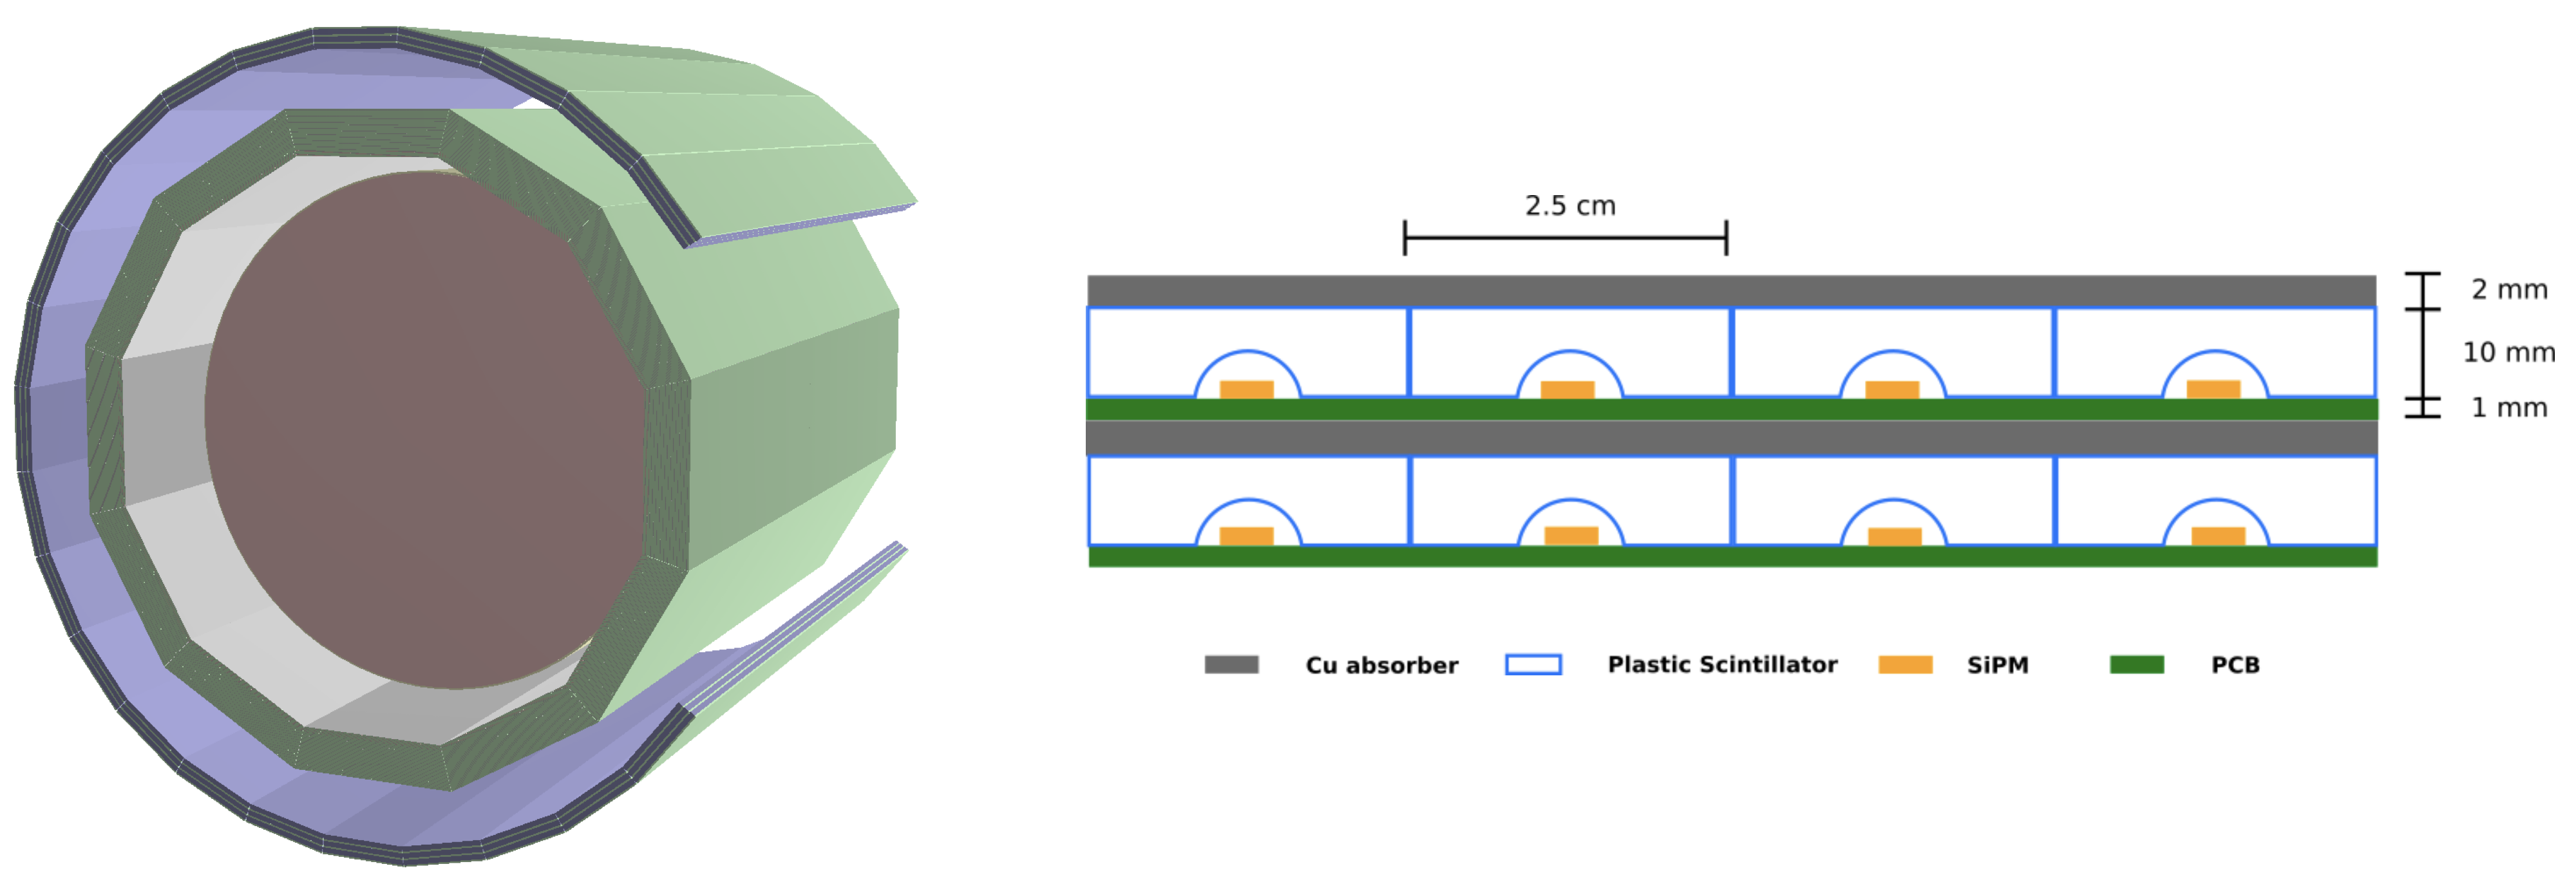
\includegraphics[width=0.99\linewidth]{Images/ND-GAr/ndgar_ecal}
	\caption[Diagram of the ALICE TPC, showing the two drift chambers, inner and outer field cages and readout chambers.]{View of the 12-sided ECal barrel and outer muon tagger geometries (left) and layout of the ECal tile layers for the $2~\mathrm{mm}$ Cu, $10~\mathrm{mm}$ scintillator option (right). Figure adapted from Ref. \cite{DUNE2020TDR1}.}
	\label{fig:ndgar_ecal}
\end{figure}

The main role of the ND-GAr ECal is the calorimetric measurement of the electron energies and the reconstruction of photons, in particular those from neutral pion decays. Also, the ECal is able to provide a $t_{0}$ timestamp for neutrino interactions, by associating its activity to the tracks in the HPgTPC. The ECal will also be able to perform neutron reconstruction using time of flight and reject external backgrounds, thanks to its sub-nanosecond time resolution.

The ECal design features three independent subdetectors, two end caps at each side and a barrel surrounding the HPgTPC. Each of the detectors is divided in modules, which combine alternating layers of plastic scintillator and absorber material readout by SiPMs. The inner scintillator layers consist of $2.5\times2.5~\mathrm{cm}^{2}$ high-granularity tiles, whereas the outer ones are made out of $4~\mathrm{cm}$ wide cross-strips spanning the whole module length. The current barrel geometry consists of 8 tile layers and 34 strip layers, while the end caps feature 6 and 36 respectively. The thickness of the scintillator layers is $7~\mathrm{mm}$ and $5~\mathrm{mm}$ for the Pb absorber layers. The 12-sided geometry of the ECal barrel (left) and the layout of the tile layers (left)\footnote{The figure shows the layout of the tile layers for a previous design with $2~\mathrm{mm}$ Cu absorber and $10~\mathrm{mm}$ plastic scintillator, as mentioned in the text the current choice is $5~\mathrm{mm}$ Pb absorber and $7~\mathrm{mm}$ scintillator.} can be seen in Fig. \ref{fig:ndgar_ecal}.

\subsection{Magnet}

The ND-GAr magnet design, know as the Solenoid with Partial Yoke (SPY), consists of two coupled solenoids with an iron return yoke. The idea behind the design is to have a solenoid as thin as possible, as well as a return yoke mass distribution that minimises the material budget between ND-LAr and ND-GAr. The magnet needs to provide a $0.5~\mathrm{T}$ field in the direction perpendicular to the beam, parallel to the drift electric field. It needs to host the pressure vessel and the surrounding ECal, which points to a inner diameter of $\sim6.4~\mathrm{m}$.

The solenoid is a single layer coil, based on niobium titanium superconducting Rutherford cable. The total length of the coil is $7.5~\mathrm{m}$. The bobbin will be split in four segments grouped in pairs with two identical cryostats, connected in series. The iron yoke features an aperture in the upstream side to allow the muons coming from ND-LAr. Still, its material will be enough to reduce the magnetic field reaching SAND, and also stop the charged pions produced inside the HPgTPC.

\subsection{Muon system}

The design of the ND-GAr muon system is still in a preliminary stage. Its role is to distinguish between muons and pions punching through the ECal. This is especially important for wrong-sign determination, to separate these from neutral current events.

In its current form, the muon system consists of three layers of longitudinal sampling structures. It alternates $10~\mathrm{cm}$ Fe absorber slabs with $2~\mathrm{cm}$ plastic scintillator strips. The transverse granularity required is still under study.

\section{GArSoft}

GArSoft is a software package developed for the simulation and reconstruction of events in ND-GAr. It is inspired by the LArSoft toolkit used for the simulation of LArTPC experiments, like the DUNE FD modules. It is based on \texttt{art}, the framework for event processing in particle physics experiments \cite{ART}. Other of its main dependencies are \texttt{ROOT}, \texttt{NuTools}, \texttt{GENIE} and \texttt{Geant4}. It allows the user to run all the steps of a generation-simulation-reconstruction workflow using FHiCL configuration files.

\subsection{Event generation}

The standard generator FHiCLs in GArSoft run the event generation and particle propagation simulation (i.e. Geant4) in the same job by default. However, it is possible to split them up if needed. The current version of GArSoft provides five different event generators, each of them producing \texttt{simb::MCTruth} products defined in \texttt{NuTools}. The available modules are:
\begin{itemize}
	\item \texttt{SingleGen}: particle gun generator. It produces the specified particles with a given distribution of momenta, initial positions and angles.
	\item \texttt{TextGen}: text file generator. The input file must follow the \texttt{hepevt} format\footnote{In brief, each event contains at least two  lines.  The first line contains two entries, the event number and the number of particles in the event. Each following line contains 15 entries to describe each particle. The entries are: status code, pdg code for the particle, entry of the first mother for this particle, entry of the second mother for this particle, entry of the first daughter for this particle, entry of the second daughter for this particle, x component of the particle momentum, y component of the particle momentum, z component of the particle momentum, energy of the particle, mass of the particle, x component of the particle initial position, y component of the particle initial position, z component of the particle initial position and time of the particle production.}, the module simply copies this to \texttt{simb::MCTruth} data products.
	\item \texttt{GENIEGen}: GENIE neutrino event generator. The module runs the neutrino-nucleus interaction generator using the options specified in the driver FHiCL file (flux file, flavour composition, number of interactions per event, $t_{0}$ distribution, ...). Current default version is \texttt{v3_04_00}.
	\item \texttt{RadioGen}: radiological generator. It produces a set list of particles to model radiological decays. Not tested.
	\item \texttt{CRYGen}: cosmic ray generator. The module runs the CRY event generator with a configuration specified in the FHiCL file (latitude and altitude of detector, energy threshold, ...). Not tested.
\end{itemize}

The module \texttt{GArG4} searches for all the generated \texttt{simb::MCTruth} data products, using them as inputs to the Geant4 simulation with the specified detector geometry. A constant $0.5~\mathrm{T}$ magnetic field along the drift coordinate is assumed. The main outputs of this step are \texttt{simb::MCParticle} objects for the generated Geant4 particles, \texttt{gar::EnergyDeposit} data products for the energy deposits in the HPgTPC and \texttt{gar::CaloDeposit} data products for the energy deposits in the ECal and muon system.

\subsection{Detector simulation}

The standard detector simulation step in GArSoft is all run with a single FHiCL, but the different modules can be run independently as well. First the \texttt{IonizationReadout} module simulates the charge readout of the HPgTPC, and later the \texttt{SiPMReadout} module runs twice, once for the ECal and then for the muon system, with different configurations.

The \texttt{IonizationAndScintillation} module collects all the \texttt{gar::EnergyDeposit} data products, to compute the equivalent number of ionization electrons for each energy deposit. The \texttt{ElectronDriftAlg} module simulates the electron diffusion numerically both in the longitudinal and transverse directions and applies an electron lifetime correction factor. The induced charge on the nearest and neighbouring readout pads is modeled using the provided pad response functions. The digitisation of the data is then simulated with the \texttt{TPCReadoutSimAlg} module. By default, the ADC sampling rate used is $50.505~\mathrm{MHz}$. The resulting raw waveforms for each channel are stored with zero-suppression, in order to save memory and CPU time. The algorithms keep blocks of ADC values above a certain threshold, plus some adjustable additional early and late tick counts. The results of these three steps are \texttt{gar::raw::RawDigit} data products.

For the ECal and the muon system the \texttt{SiPMReadout} module calls either the \texttt{ECALReadoutSimStandardAlg} or \texttt{MuIDReadoutSimStandardAlg} modules. These take all the \texttt{gar::CaloDeposit} data products in the corresponding detector and do the digitisation depending on whether the hit was in a tile or strip layer. They include single photon statistics, electronic noise, SiPM saturation and time smearing. The resulting objects are \texttt{gar::raw::CaloRawDigit} data products.

\subsection{Reconstruction}

The reconstruction in GArSoft is also run as a single job by default. It first runs the hit finding, clustering, track fitting and vertex identification in the HPgTPC, followed by the hit finding and clustering in the ECal and muon system. After those it produces the associations between the associations between the tracks and the ECal clusters.

Focusing first on the HPgTPC reconstruction, the \texttt{CompressedHitFinder} module takes the zero-suppressed ADCs from the \texttt{gar::raw::RawDigit} data products. The reconstructed hits largely correspond to the above threshold blocks, however the hit finder identifies waveforms with more than one maximum, diving them in multiple hits if they dip below a certain threshold. The data products produced are of the form \texttt{gar::rec::Hit}. These are the inputs to the clustering of hits in the \texttt{TPCHitCluster} module. Hits close in space and time are merged, and the resulting centroids are found. This module outputs \texttt{gar::rec::TPCClusters} objects and associations to the input hits.

The following step prior to the track fitting is pattern recognition. The module called \texttt{tpcvechitfinder2} uses the \texttt{gar::rec::TPCClusters} data products to find track segments, typically called vector hits. They are identified by performing linear 2D fits to the positions of the clusters in a $10~\mathrm{cm}$ radius, one fit for each coordinate pair. A 3D fit defines the line segment of the vector hit, using as independent variable the one whose sum of (absolute value) slopes in the 2D fits is the smallest. The clusters are merged to a given vector hit if they are less than $2~\mathrm{cm}$ away from the line segment. The outputs are \texttt{gar::rec::VecHit} data products, as well as associations to the clusters. The \texttt{tpcpatrec2} module takes the \texttt{gar::rec::VecHit} objects to form the track candidates. The vector hits are merged together if their direction matches, their centers are within $60~\mathrm{cm}$ and their direction vectors point roughly to their respective centers. Once the clusters of vector hits are formed they are used to make a first estimation of the track parameters, simply taking three clusters along the track. The module produces \texttt{gar::rec::Track} data products and associations between these tracks and the clusters and vector hits.

The track is fitted by means of a Kalman filter in the \texttt{tpctrackfit2} module, using the position along the drift direction as the independent variable. Two different fits are performed per track, a forward and a backwards fit, each starting from one of the track ends. The Kalman filter state vector $(y,z,R,\phi,\mathrm{tan}\lambda)$ is estimated at each point along the track using a Bayesian update. The track parameters reported in the forward and backwards fits are the ones computed at the opposite end where the fit started. The main outputs of the track fit are the \texttt{gar::rec::Track} objects. Additionally, the module stores the fitted 3D positions along the track in the \texttt{gar::rec::TrackTrajectory} data products and the total charge and step sizes for each point also get stored in the form of \texttt{gar::rec::TrackIonization} objects.

After the tracking step, the \texttt{vertexfinder1} module looks at the reconstructed \texttt{gar::rec::Track} products, creating vertex candidates with the track ends that are within $12~\mathrm{cm}$ of each other. The vertices are then fitted using linear extrapolations from the different track ends associated. The results are \texttt{gar::rec::Vertex} data products, and associations to the tracks and corresponding track ends.

For the ECal and muon tagger, the \texttt{SiPMHitFinder} module runs twice with different configurations, adapted to the particular capabilities of both. The module simply takes the \texttt{gar::raw::CaloRawDigit} products, applies a calibration factor to convert the ADC counts to $\mathrm{MeV}$ and for the strip layer hits it calculates the position along the strip using the times recorded of both SiPMs. This module produces \texttt{gar::rec::CaloHit} data products. Next, these objects are used as inputs to the \texttt{CaloClustering} module. It merges the hits based on a simple nearest neighbours (NN) algorithm. For the resulting clusters it also computes the total energy and position of the centroid. The results are stored as \texttt{gar::rec::Cluster} data products, with associations to the hits.

The last step in the reconstruction is associating the reconstructed tracks in the HPgTPC to the clusters formed in the ECal and muon system. The \texttt{TPCECALAssociation} module checks first the position of the track end points, considering only the points that are at least $215~\mathrm{cm}$ away from the cathode or have a radial distance to the center greater than $230~\mathrm{cm}$. The candidates are propagated up to the radial position, in the case of clusters in the barrel, or the drift coordinate position, for the end cap cluster, of the different clusters in the collection using the track parameters computed at the end point. The end point is associated to the cluster if certain proximity criteria are met. This module creates associations between the tracks, the end points and the clusters. The criteria for the associations are slightly different for the ECal and the muon tagger.
%\chapter{FWTPG offline software}
\label{chapter:fwtpg_software}

\chapter{Matched Filter approach to Trigger Primitives}\label{chapter:matched_filter}

\begin{chapquote}{Arthur Conan Doyle, \textit{A scandal in Bohemia}}
	It is a capital mistake to theorize before one has data. Insensibly one begins to twist facts to suit theories, instead of theories to suit facts.
\end{chapquote}

The DAQ system is responsible for the data that will be collected in the DUNE FD. Therefore, it has the capability of either expanding or limiting our physics reach, depending of its specifications. This is important for the low energy physics programme, as it requires more sensitive and reliable methods to pick up the relevant signals.

In this Chapter, I present a novel method to improve the sensitivity of the DUNE FD by enhancing the production of hits in the online processing. This is possible thanks to a more efficient filtering strategy, the matched filter, which benefits the induction channels of the detector.

\section{Motivation}
\label{sec:matched_filter_motivation}

The lowest-level objects that are formed within the DUNE FD DAQ system are the so-called trigger primitives (TPs) \cite{DUNEDAQ2022}. These represent the hits on a channel, and are used as input to the rest of the DAQ trigger chain. The TPs are formed in the hit finder chain. A schematic representation of it is shown in Fig. \ref{fig:tpg_chain}. This chain takes the raw ADC data from the detector, removes the constant pedestal of the signal using a dynamical median estimation method, applies a filter to the waveform, and tries to find peaks over a certain threshold. These peaks form the TPs, which contain information such as the start and end times over the threshold, the maximum ADC value and the corresponding ADC integral. Currently, there are two implementations of the hit finder chain, one firmware-based and other software-based.

The filter implemented in the firmware of the upstream DUNE FD DAQ is a $32$nd-order low-pass finite impulse-response (FIR) filter. The output of such filter for a discrete system can be written as:
\begin{equation}\label{2.1.1}
	y[i] = \sum_{j=0}^{N} h[i] x[i-j],
\end{equation}
where $N$ is the order of the filter, $y$ is the output sequence, $x$ is the input sequence and $h$ is the set of filter coefficients. The current implementation within \texttt{dtp-firmware} \cite{dtp-firmware} uses a set of 16 non-zero integer coefficients. For the software case, only a 5th-order filter is used, as the filtering is the most CPU-expensive part of the software hit finder.

Filtering is a vital step in the hit finder chain. It helps suppressing the noise and enhances the signal peaks with respect to the noiseless baseline. A good filtering strategy allows us to use lower thresholds when forming the TPs, thus increasing the sensitivity of our detector to low energy physics events. In such events, the hits produced by the ionisation electrons tend to have lower amplitudes than those of interest to the LBL physics programme of the DUNE experiment.

\begin{figure}[t]
	\centering
	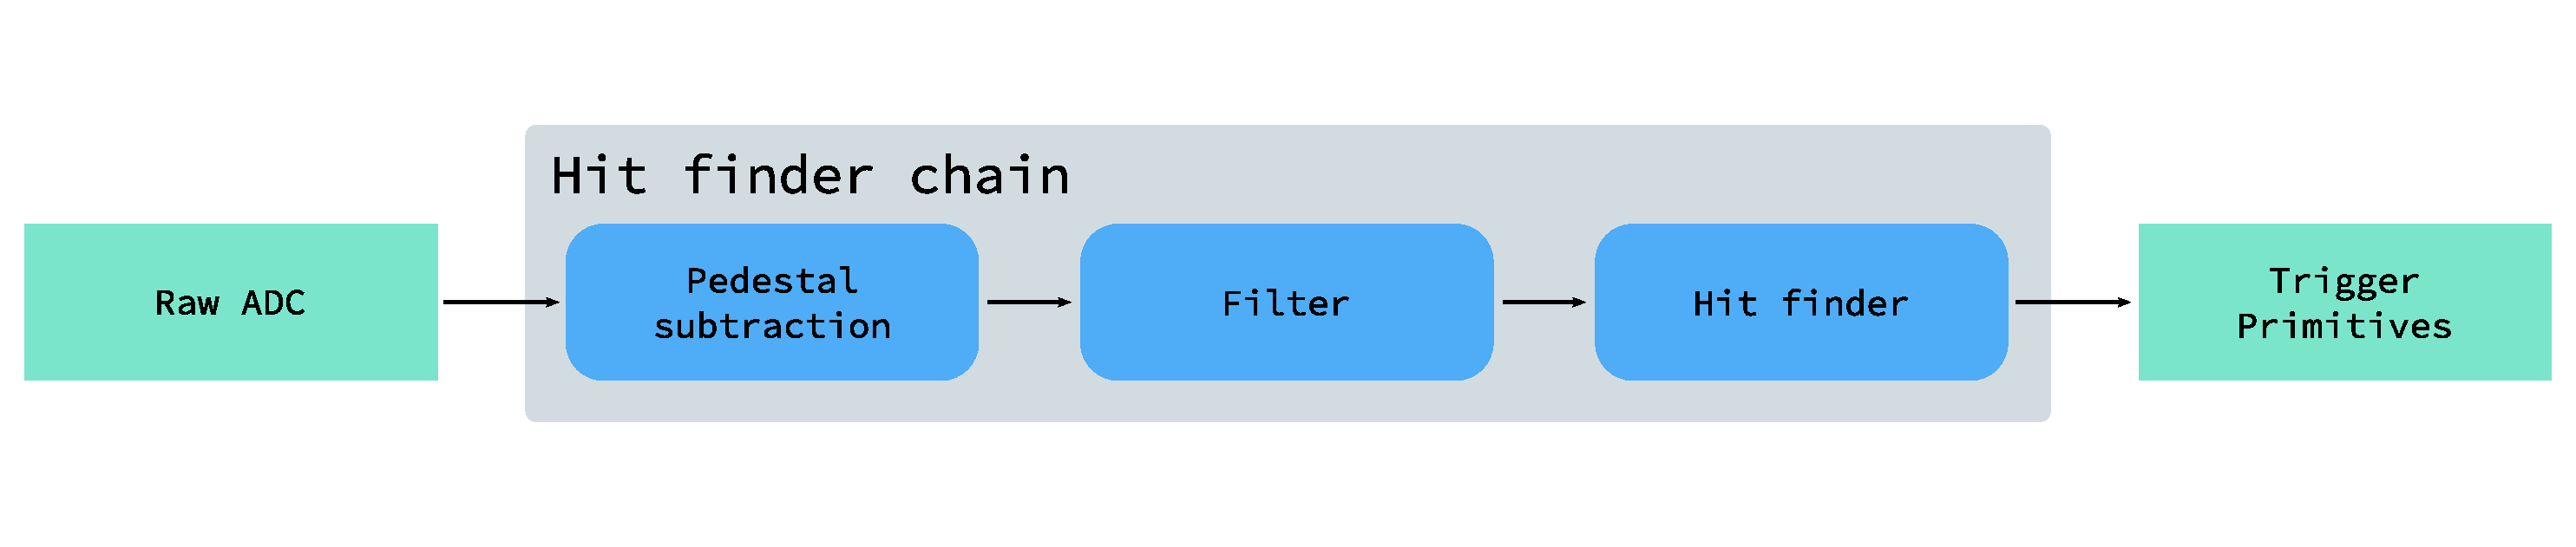
\includegraphics[width=0.99\linewidth]{Images/Matched_Filter/trigger_primitive_chain.pdf}
	\caption{Schematic representation of the Trigger Primitive Generation chain in the DUNE FD.}
	\label{fig:tpg_chain}
\end{figure}

This is particularly important for the induction planes. In general, signal peaks in the induction channels have smaller amplitude than the ones in the collection plane. This, together with the fact that the pulse shapes are bipolar, reduces our capacity to detect the hits on these channels. The inefficiency of detecting TPs in the induction planes (denoted as U and V planes) leads trigger algorithms to focus mainly on the TPs from the collection plane (so-called X plane). As a result, the possibility of making trigger decisions based on the coincidence of TPs across the three wire planes remains nowadays unexploited in DUNE. This will be beneficial for low energy events, as it adds redundancy to the algorithms, as well as for other physics that requires online directionality information, like the supernova pointing.

A possible improvement of the current hit finder chain may require optimising the existing or choosing a new filter implementation. A filter strategy which benefits the induction signals may be able to enhance the detection efficiency of TPs from the induction planes and ideally make it comparable to that of the collection plane.  

The goal is to implement a better finite-impulse response filter and to evaluate its performance relative to the current filter. To do so, I need to take into account the limitations of the firmware: the FIR filter shall have maximum 32 coefficients (so-called taps) whose values are 12-bit unsigned integers. Although it is technically possible to include non-integer coefficients, it would be a technical challenge. For instance, in the HD design there are 40 FIR instances per APA, as there are 4 FIR blocks per optical link and 10 optical links per APA. Therefore, the impact of increasing the complexity of the filter will be amplified forty times in the FPGA load. With these restrictions, the task is to provide a set of 32 coefficients which yield an optimal filter performance for the induction channels. A solution compatible with the software hit finder implementation is not considered, due to its current limitations concerning the filtering stage.

\section{Signal-to-noise ratio definition}
\label{sec:matched_filter_sn_definition}

\begin{figure}[t]
	\centering
	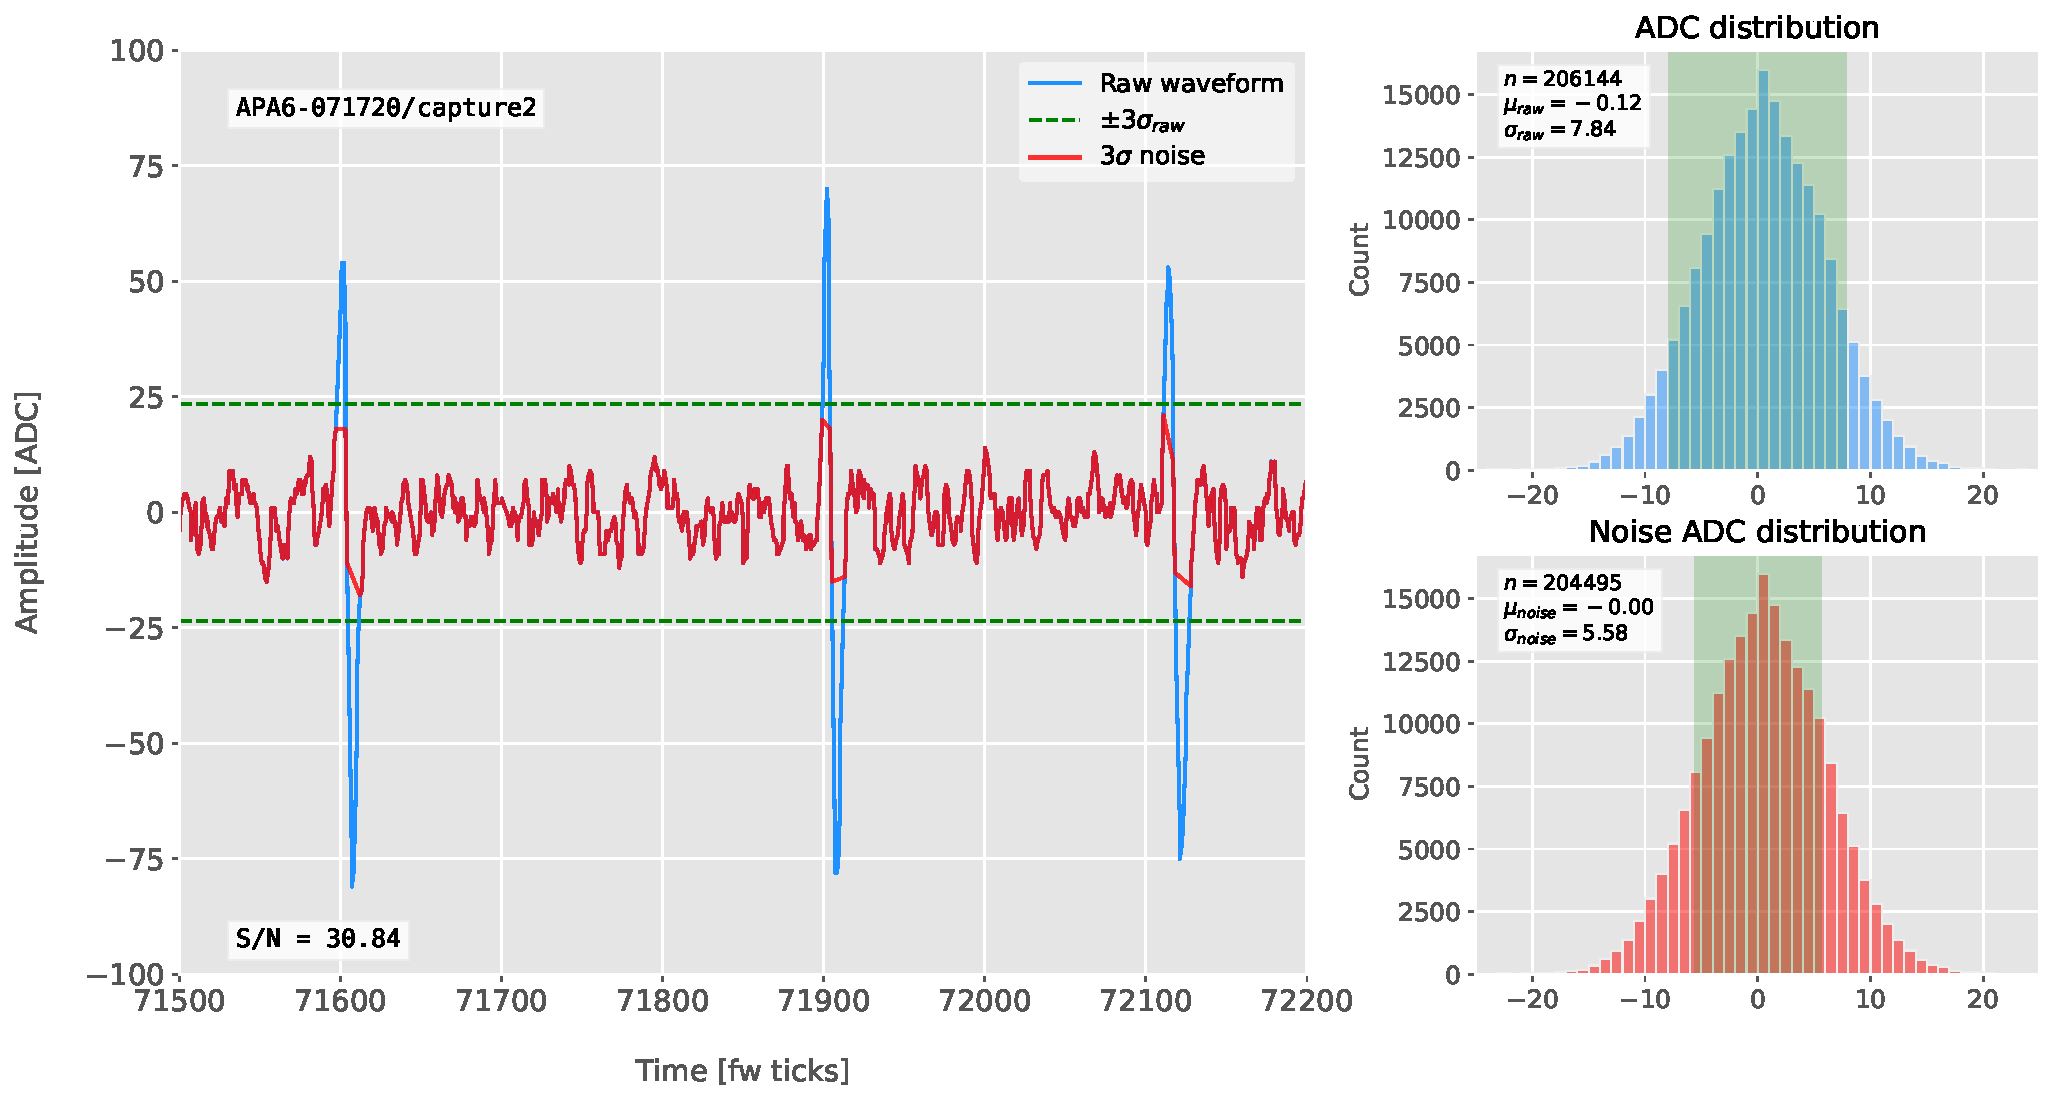
\includegraphics[width=1\linewidth]{Images/Matched_Filter/waveform_example_raw}
	\caption[Example unfiltered waveform from a ProtoDUNE-SP raw data capture.]{Left panel: Zoomed unfiltered waveform corresponding to channel $7840$ from the ProtoDUNE-SP raw data capture \texttt{felix-2020-07-17-21:31:44} (blue line). The green dashed lines mark the region $\pm3\sigma_{raw}$. The resulting noise waveform is also shown (red line). Top right panel: ADC distribution for channel $7840$, where the green shaded region represents $\pm \sigma_{raw}$. Bottom right panel: noise ADC distribution for channel $7840$, where the green shaded region represents $\pm \sigma_{noise}$.}
	\label{fig:adcs_nofir}
\end{figure}

In the following, I use the signal to noise ratio (S/N) as a measure of the FIR filter performance. The S/N metrics allow us to compare different filter implementations and serve as a basis for more detailed studies presented later in this Chapter. Here, I demonstrate how to extract its value for a set of 
ProtoDUNE-SP data. Specifically, I use the ADC capture \texttt{felix-2020-07-17-21:31:44}, a raw data capture taken for firmware validation purposes. I define the S/N of a channel as the height of the signal peaks relative to the size of the noise. To quantify this, I first estimate the standard deviation of the ADC data for each channel, $\sigma_{\mathrm{ADC}}$. Then, I define the corresponding noise waveform to be the ADC values in the range $\pm 3~\sigma_{\mathrm{ADC}}$. From this new noise data I compute the mean and standard deviation, $\mu_{noise}$ and $\sigma_{noise}$, so I can write the S/N for any given channel as:
\begin{equation}
	\mathrm{S/N} = \frac{\max{[\mathrm{ADC}]} - \mu_{noise}}{\sigma_{noise}},
\end{equation}
where $\max{[\mathrm{ADC}]}$ is simply the maximum ADC value found in the corresponding channel.

As an example, I apply this definition of the S/N to a waveform from one of the channels of the data capture. Figure \ref{fig:adcs_nofir} shows a zoomed region of the waveform corresponding to channel $7840$ (blue line), where one can clearly see three signal peaks and continuous additive noise\footnote{There are actually 6 peaks, 3 positive and 3 negative, but, because by design for induction channels the expected signal pulse shapes are bipolar, we treat them as a collection of 3 individual signals.}. I estimated the standard deviation of this raw waveform to be $\sigma_{raw} = 7.84 ~ \mathrm{ADC}$, and from this I am able to define the noise waveform (red line) as the ADC values in the range $\pm 23.52 ~ \mathrm{ADC}$. This way, I obtain $\mu_{noise} = 0.01 ~ \mathrm{ADC}$ and $\sigma_{noise} = 5.58 ~ \mathrm{ADC}$, which gives $\mathrm{S/N} = 30.84$.

I repeat this calculation now for the corresponding filtered waveform, using the current firmware FIR filter. Figure \ref{fig:adcs_fir} shows the same time window for the filtered waveform from channel $7840$ (blue line). In this case, the standard deviation of the waveform is larger than before, giving $\sigma_{raw} = 10.99 ~ \mathrm{ADC}$. The noise waveform (red line) is formed by selecting the ADC values in the $\pm 32.91 ~ \mathrm{ADC}$ range, which gives $\mu_{noise} = -0.47 ~ \mathrm{ADC}$ and $\sigma_{noise} = 7.03 ~ \mathrm{ADC}$. Finally, one obtains $\mathrm{S/N} = 24.68$. Notice that the value of S/N decreases after the filtering. Clearly, one can see that the noise baseline has increased by a factor of $1.35$ when we applied the FIR filter, and at the same time the amplitude of the signal peaks has remained almost unchanged, leading to this poorer S/N value.

\begin{figure}[t]
	\centering
	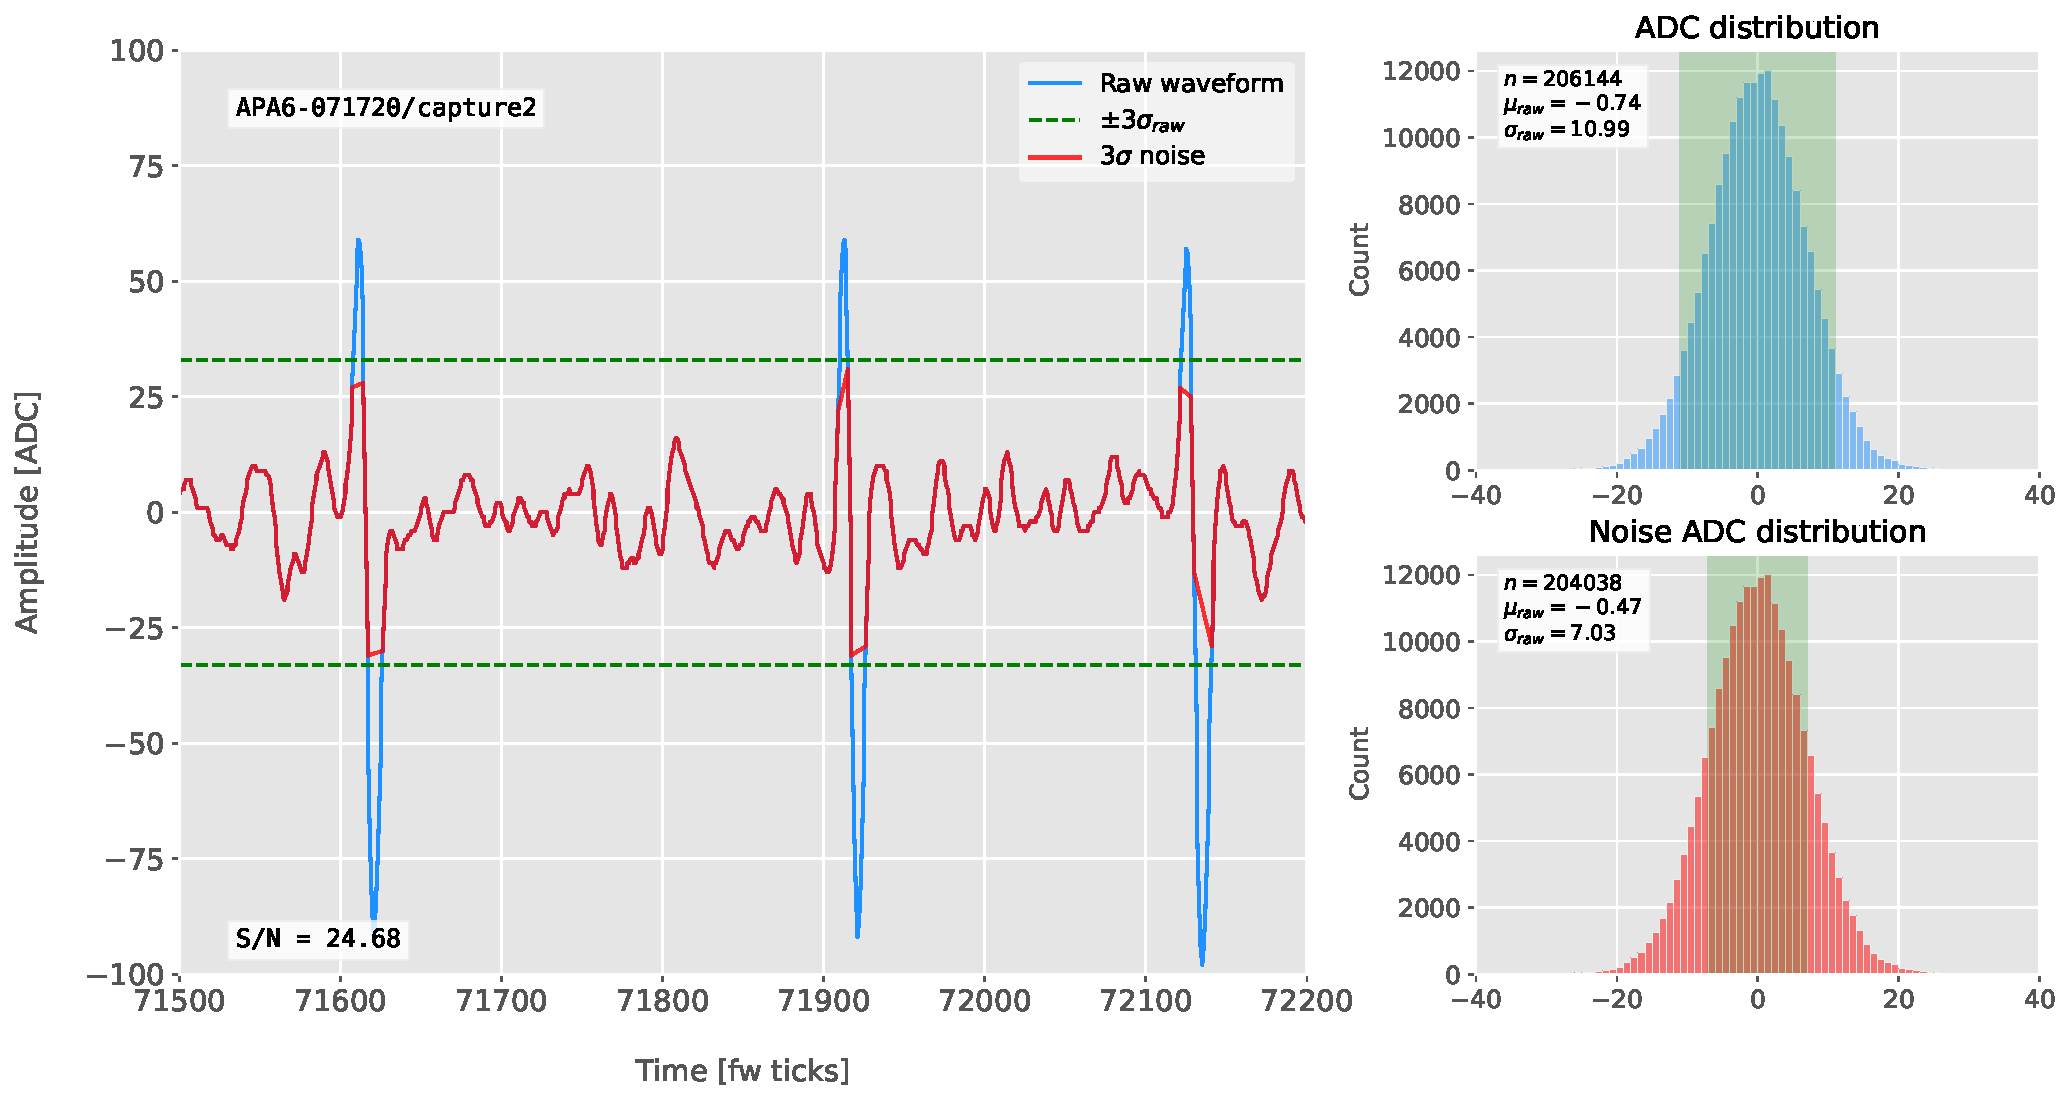
\includegraphics[width=1\linewidth]{Images/Matched_Filter/waveform_example_fir}
	\caption[Example filtered waveform from a ProtoDUNE-SP raw data capture.]{Left panel: Zoomed filtered waveform corresponding to channel $7840$ from the ProtoDUNE-SP raw data capture \texttt{felix-2020-07-17-21:31:44} (blue line). The filter used was the current implementation of the low-pass FIR filter in \texttt{dtp-firmware}. The green dashed lines mark the region $\pm3\sigma_{raw}$. The resulting noise waveform is also shown (red line). Top right panel: ADC distribution for channel $7840$ after filtering, where the green shaded region represents $\pm \sigma_{raw}$. Bottom right panel: noise ADC distribution for channel $7840$ after filtering, where the green shaded region represents $\pm \sigma_{noise}$.}
	\label{fig:adcs_fir}
\end{figure}

\section{Low-pass FIR filter design}
\label{sec:matched_filter_fir}

To optimise the frequency response of a digital filter, we can use the Parks-McClellan algorithm, where one finds a set of $N$ real coefficients that give the best response for the specified pass-band and order of the filter \cite{McClellan2005}.

Taking the detector ticks as the time unit, the Nyquist frequency will simply be $1/2 \ \mathrm{ticks^{-1}}$. The current implementation of the filter seems to have as pass-band the range $[0,0.1] \ \mathrm{ticks^{-1}}$. This can be seen in Fig. \ref{fig:filter_comp}, where I show the power spectrum, in decibels, of that filter implementation (blue solid line). The Park-McClellan algorithm finds the optimal Chebyshev FIR filter \cite{Weinberg1960} taking as input the boundaries of the target pass-band and stop-band, which can be written in the form:
\begin{equation}
	\left\{ \begin{array}{c}
		\left[0, f_{c}\right] \\
		\left[ f_{c} + \delta f, f_{N}\right]
	\end{array} \right. ,
\end{equation}
where $f_{c}$ is the cut-off frequency, $\delta f$ is the transition width and $f_{N}$ is the aforementioned Nyquist frequency. A filter with a similar behaviour to the previous one can be obtained by setting $f_{c} = 0$ and $\delta f = 0.1 \ \mathrm{ticks}^{-1}$. The response of the resulting filter is also shown in Fig. \ref{fig:filter_comp} (blue solid line). Notice that the suppression of the stop-band is enhanced for this optimal filter. For comparison, I include the power response of the filter obtained by taking the integer part of the coefficients resulting from the Parks-McClellan method (red dashed line). One can see that it does not suppress that much the stop-band, in a similar way to the current implementation of the filter.

\begin{figure}[h!]
	\centering
	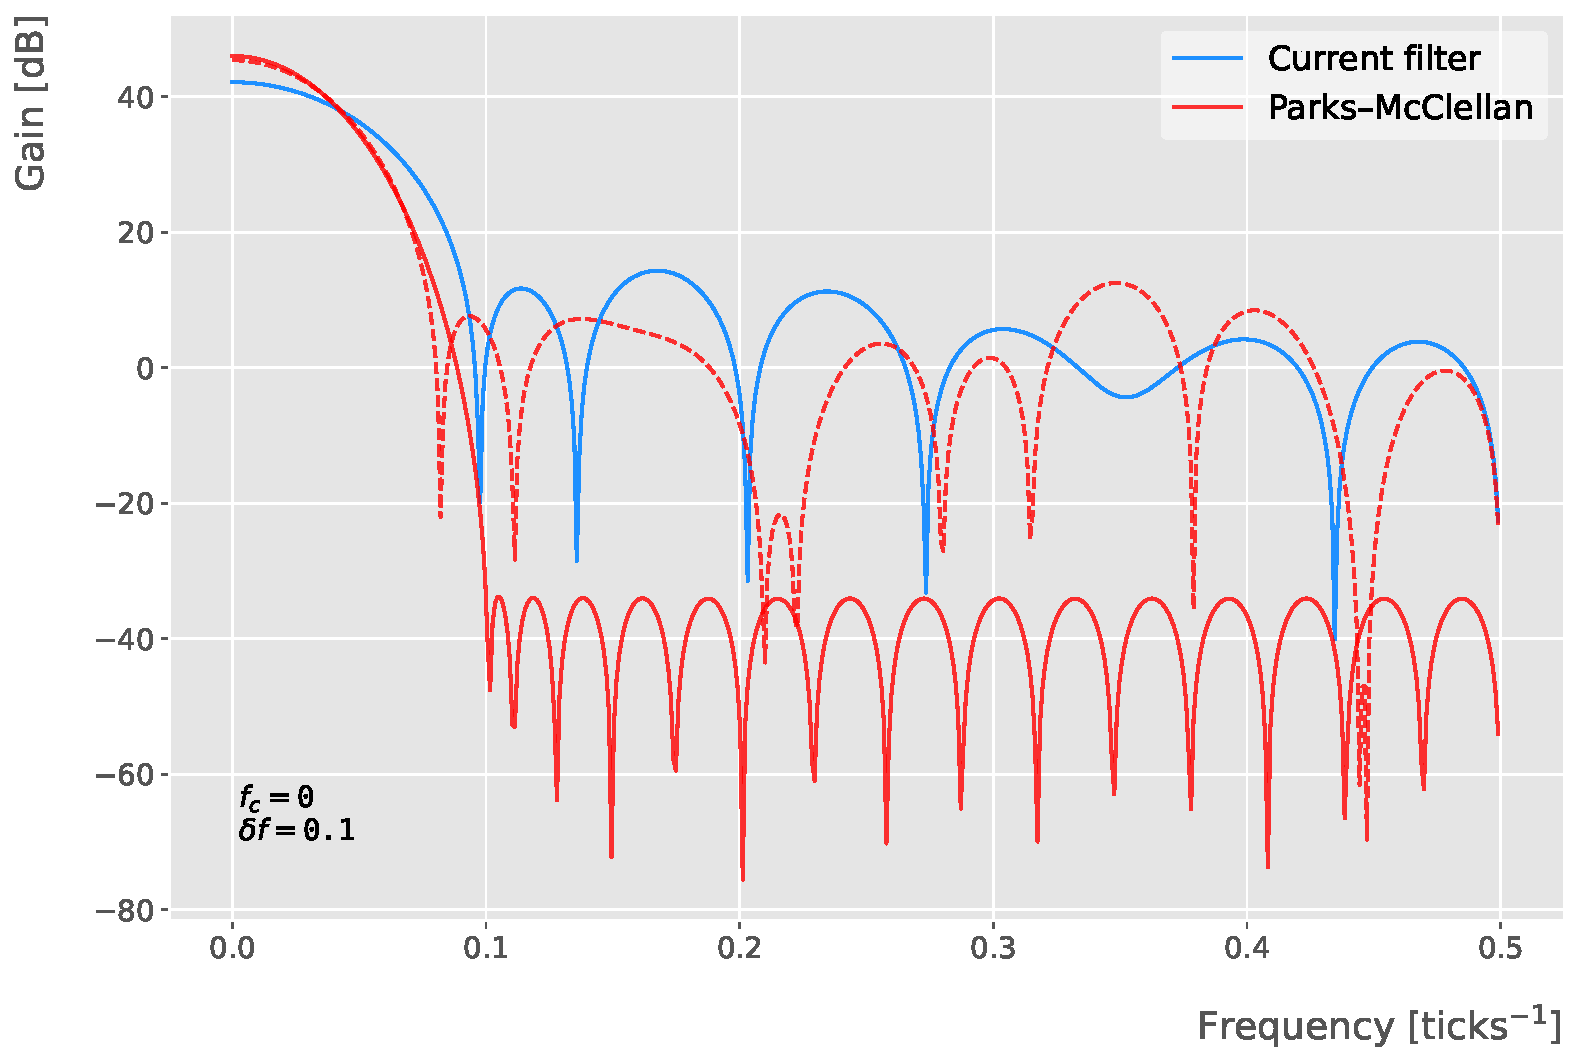
\includegraphics[width=0.8\linewidth]{Images/Matched_Filter/filter_comp}
	\caption[Power spectra for the current low-pass FIR filter and the optimal filter obtained using the Parks-McClellan algorithm.]{Power spectrum in decibels for the current implementation of the low-pass FIR filter in \texttt{dtp-firmware} (blue line), compared to the response of an optimal filter obtained using the Parks-McClellan algorithm for the same pass-band (red line). Also for comparison I include the spectrum of the optimal filter when taking only the integer part of the coefficients (red dashed line).}
	\label{fig:filter_comp}
\end{figure}

At this point, I tried to improve the performance of the FIR filter using the Park-McClellan method, i.e. maximise the overall S/N, using the available data captures. I did so by varying the values of the two quantities that parametrise the pass-band and stop-band, the cut-off frequency $f_{c}$ and the transition width $\delta f$.

\begin{figure}[t]
	\centering
	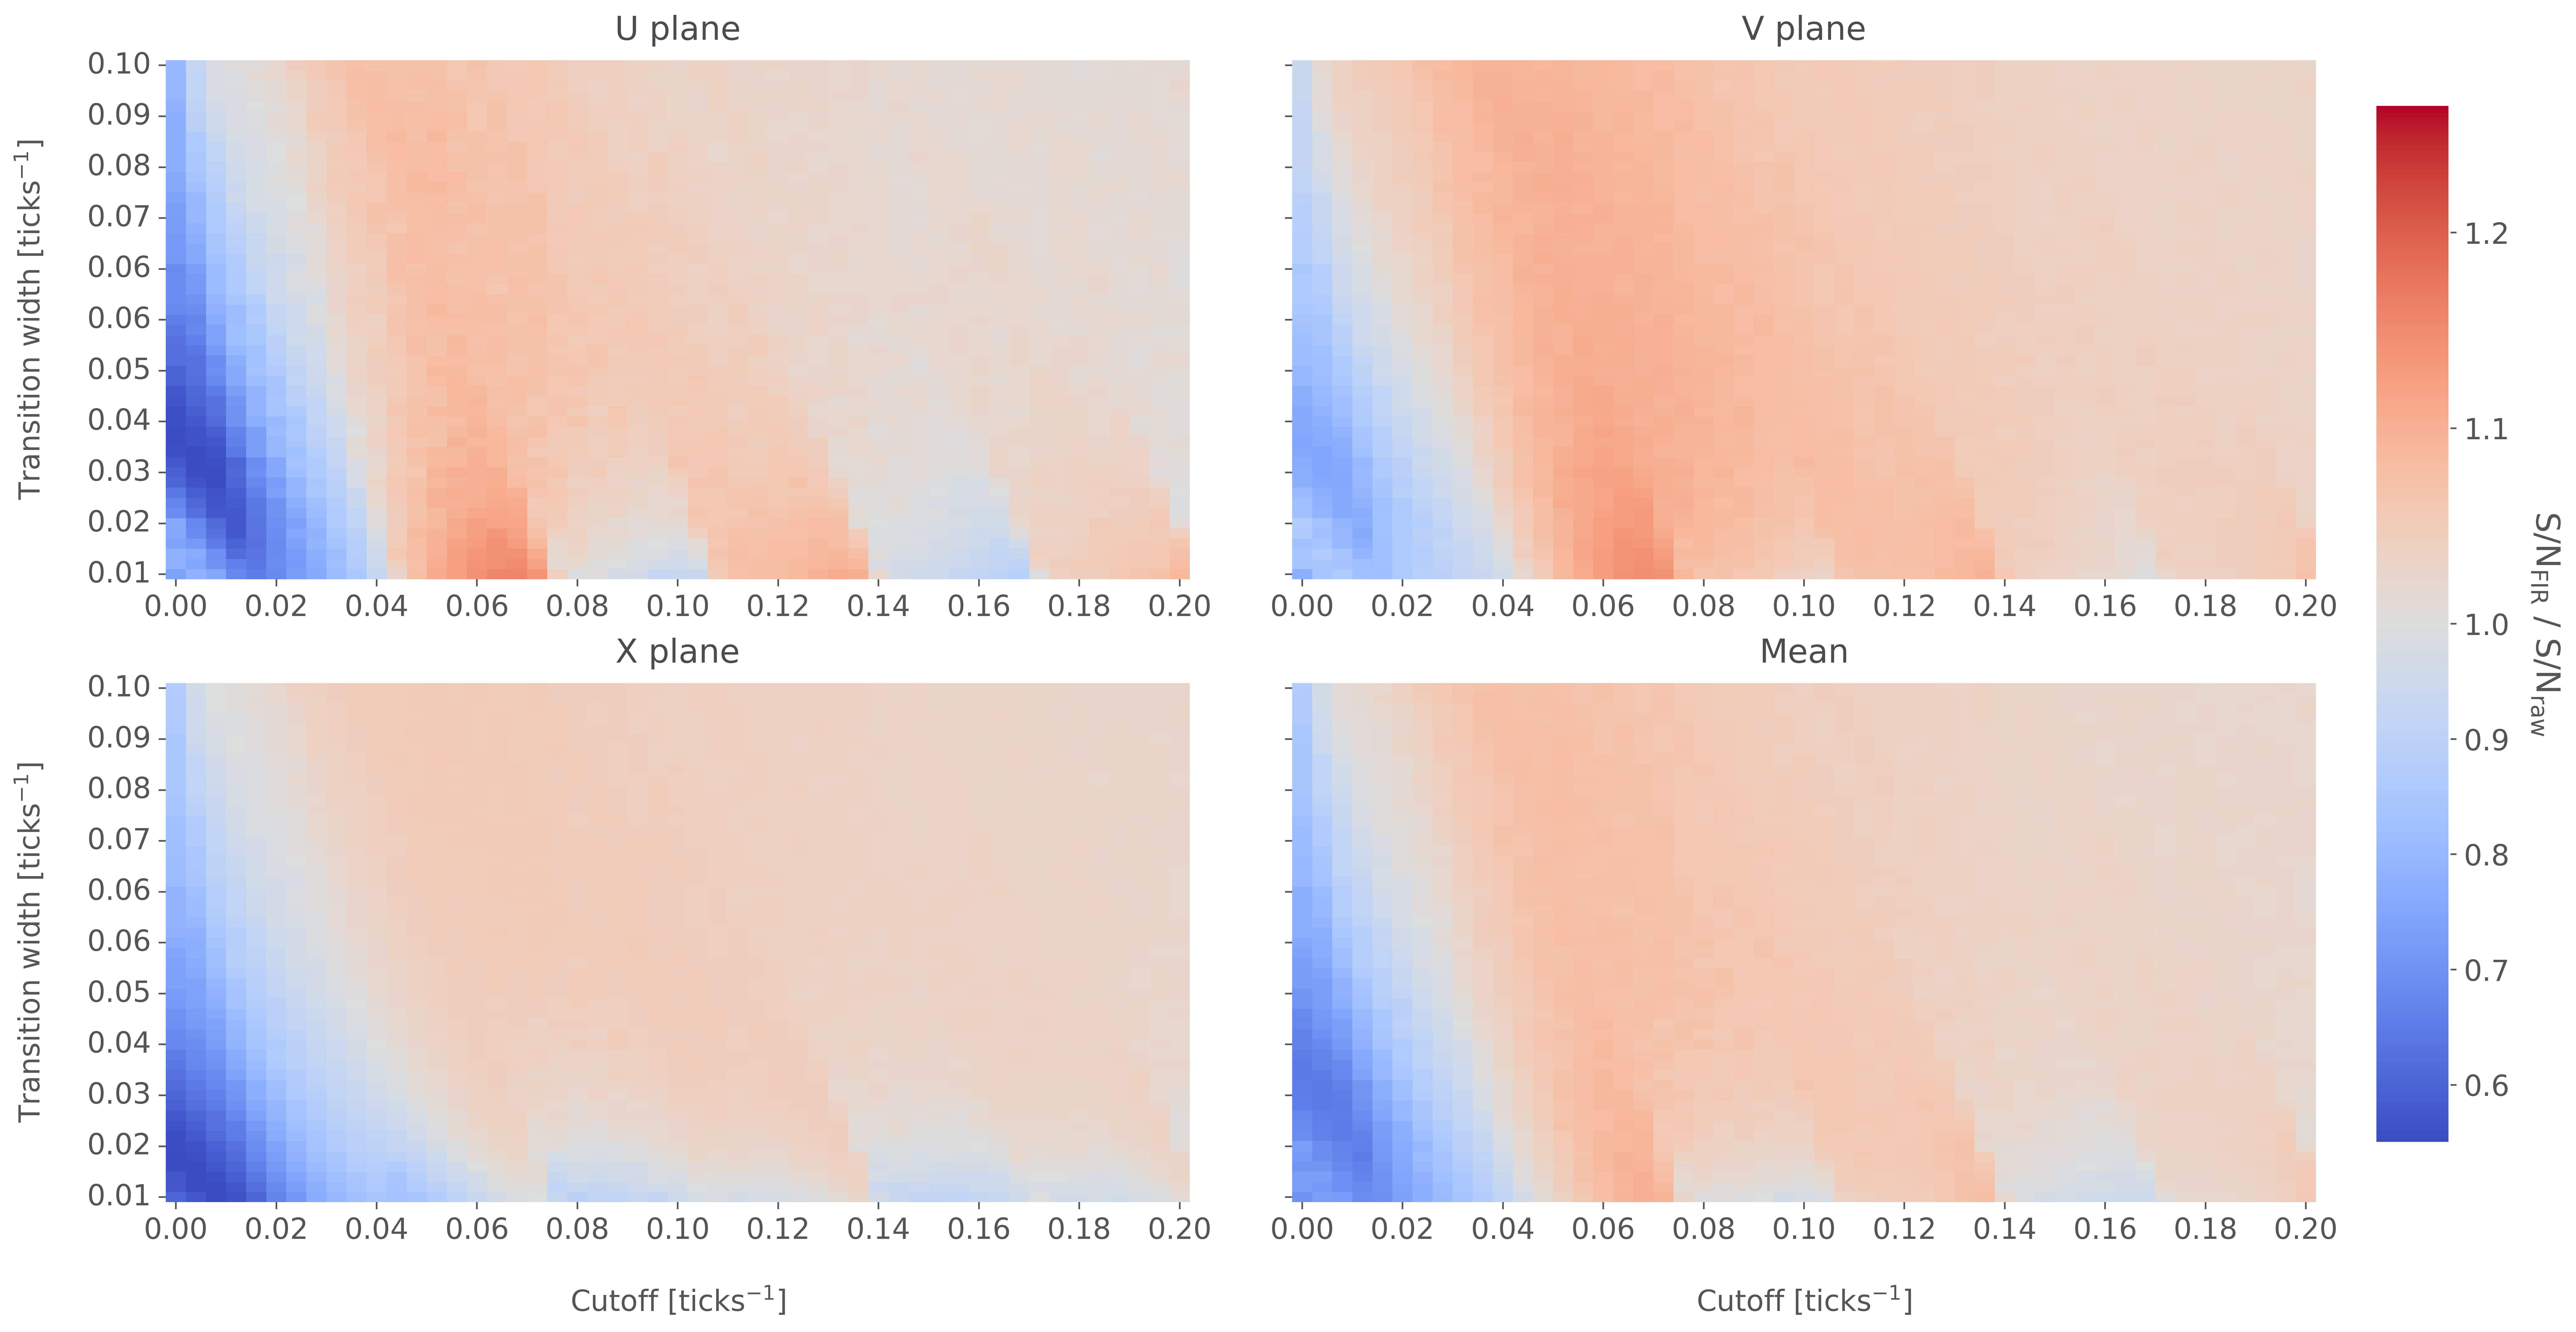
\includegraphics[width=1\linewidth]{Images/Matched_Filter/pm_fir_opt.png}
	\caption[Relative change in the S/N of the ProtoDUNE-SP raw data capture for different values of the cutoff frequency $f_{c}$ and the transition width $\delta f$.]{Relative change in the S/N for the ProtoDUNE-SP raw data capture \texttt{felix-2020-07-17-21:31:44}, using different values of the cutoff frequency $f_{c}$ and the transition width $\delta f$. The optimal Chebyshev filters were applied using just the integer part of the coefficients given by the Parks-McClellan algorithm.}
	\label{fig:fir_opt}
\end{figure}

\begin{figure}[t]
	\centering
	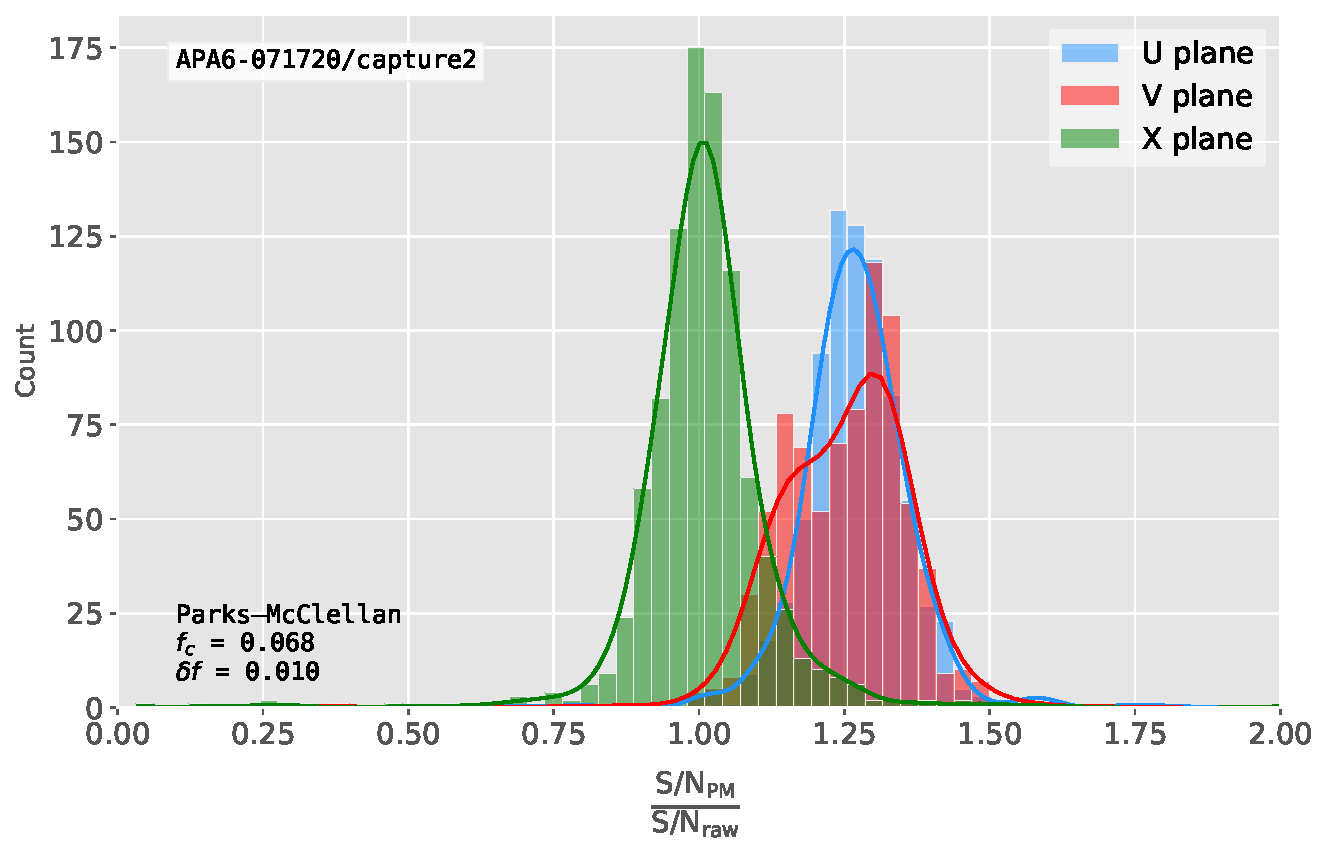
\includegraphics[width=0.85\linewidth]{Images/Matched_Filter/pm_fir_perf}
	\caption[Distribution of the relative change of the S/N on the different wire planes after the optimal FIR filter was applied.]{Distribution of the relative change of the S/N on the different wire planes from the ProtoDUNE-SP raw data capture \texttt{felix-2020-07-17-21:31:44} after the optimal Chebyshev filter was applied. The filter was computed with the Parks-McClellan algorithm using a cutoff of $f_{c} = 0.068 \ \mathrm{ticks}^{-1}$ and a transition width $\delta f = 0.010 \ \mathrm{ticks}^{-1}$.}
	\label{fig:fir_best}
\end{figure}

Figure \ref{fig:fir_opt} shows the average relative change in the S/N (i.e. the ratio between the value of the S/N after and before the filtering) for capture \texttt{felix-2020-07-17-21:31:44}, when using filters designed with the Parks-McClellan algorithm for the specified values of the cut-off frequency $f_{c}$ and the transition width $\delta f$, restricted to integer values for the filter coefficients. One can clearly distinguish different regions where we get an improvement of up to a factor of $1.35$ for the U plane. For large values of $f_{c} + \delta f$ the ratio tends to $1$, as expected. In that limit the width of the stop-band goes to $0$, meaning that no frequencies are filtered out and thus the waveform remains the same.

As it can be seen in Fig. \ref{fig:fir_opt} (bottom right panel) the configuration which gives the best mean performance for the three planes is $f_{c} = 0.068 \ \mathrm{ticks}^{-1}$ and $\delta f = 0.010 \ \mathrm{ticks}^{-1}$. We can use these to see how the filter affects the different channels. Figure \ref{fig:fir_best} shows the distribution of the S/N improvement values for all the channels in the raw ADC capture \texttt{felix-2020-07-17-21:31:44}, separated by wire plane, after the optimal Chebyshev filter was applied. One can see that there is a clear improvement for both U and V induction planes, obtaining a mean change of $1.25$ and $1.30$ for them, respectively. However, in the case of the X collection plane the distribution peaks around $1$, meaning that an important fraction of channels in that plane get a slightly worse S/N after the filter is applied. This is not a big issue, as the S/N for collection channels is usually much higher than the one for induction channels.

The results I obtained optimising the low pass filter with the Parks-McClellan method are promising. Nonetheless, the improvement found is rather marginal. Thus, I explored alternative approaches to the filtering problem, which may yield better outputs. This way, I found a possible solution in matched filters. By construction, this kind of filters offer the best improvement on the S/N.

\section{Matched filters}
\label{sec:matched_filter_matched_filter}

In the context of signal processing, a matched filter is the optimal linear filter for maximising the S/N in the presence of additive noise. It is obtained by convolving a conjugated time-reversed known template with an unknown signal to detect the presence of the template in the signal \cite{Turin1960}.

\begin{figure}[t]
	\centering
	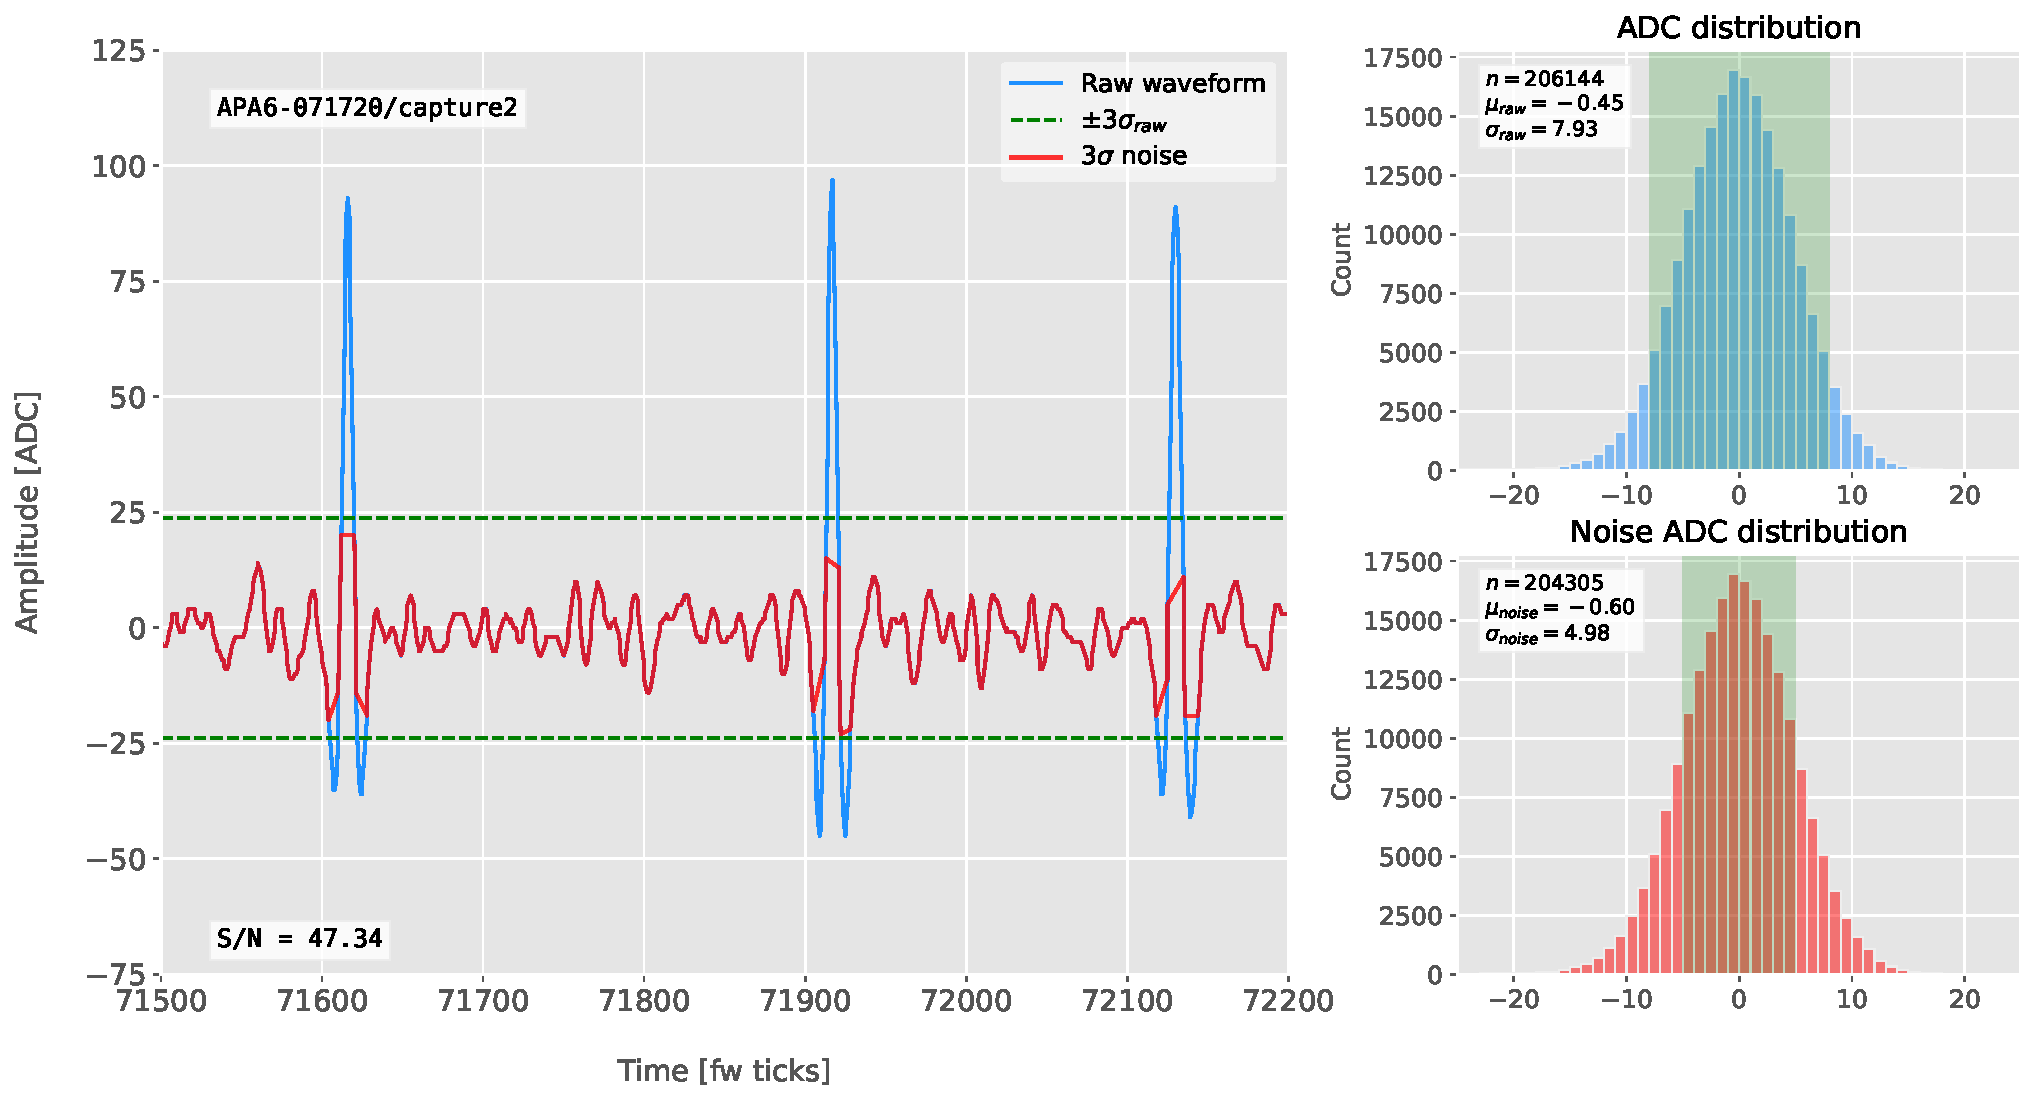
\includegraphics[width=1\linewidth]{Images/Matched_Filter/waveform_example_mf}
	\caption[Example matched filtered waveform from a ProtoDUNE-SP raw data capture.]{Left panel: Zoomed match filtered waveform corresponding to channel $7840$ from the ProtoDUNE-SP raw data capture \texttt{felix-2020-07-17-21:31:44} (blue line). The filter used was directly extracted from the data, being the $32$ values around the first peak in the original waveform. The green dashed lines mark the region $\pm3\sigma_{raw}$. The resulting noise waveform is also shown (red line). Top right panel: ADC distribution for channel $7840$ after match filtering, where the green shaded region represents $\pm \sigma_{raw}$. Bottom right panel: noise ADC distribution for channel $7840$ after match filtering, where the green shaded region represents $\pm \sigma_{noise}$}
	\label{fig:adcs_mf}
\end{figure}

Given a known signal sequence $s(t)$ and another (a priori unknown) noise sequence $n(t)$, the input signal can be written as:
\begin{equation}\label{2.4.1}
	x(t) = s(t) + n(t).
\end{equation}

Now, considering a linear time-invariant filter, whose impulse-response function I will refer to as $h(t)$, one can write the output signal as:
\begin{equation}\label{2.4.2}
	\begin{split}
		y(t) &= x(t)*h(t)\\
		&= \left(s(t) + n(t)\right)*h(t)\\
		&= y_{s}(t) + y_{n}(t),
	\end{split}
\end{equation}
where $y_{s}(t)$ and $y_{n}(t)$ are simply the outputs of the filter due to the signal and the noise components respectively.

The goal of the matched filter is to detect the presence of the signal $s(t)$ in the input sample $x(t)$ at a certain time $t_{0}$, which effectively means that we need to maximise the S/N at that given time. This way, what one wants is to have a filter which gives a much bigger output when the known signal is present than when it is not. Putting it in other words, the instantaneous power of the signal output $y_{s}(t)$ should be much larger than the average power of the noise output $y_{n}(t)$ at some time $t_{0}$.

For the case of the filtered signal, one can easily re-write it as an inverse Fourier transform:
\begin{equation}\label{2.4.3}
	y_{s}(t) = \frac{1}{2\pi} \int_{-\infty}^{\infty} \mathrm{d}\omega \ H(\omega) S(\omega) \mathrm{e}^{i \omega t},
\end{equation}
where $H(\omega)$ and $S(\omega)$ are the Fourier transforms of the impulse-response function (i.e. the transfer function of the filter) and of the input signal, respectively.

Now, focusing on the noise part, we can use the Wiener-Khinchin theorem \cite{Goodman1985} to write the mean power of the noise after filtering as:
\begin{equation}\label{2.4.4}
	E|y_{n}(t)|^{2} = \frac{1}{2\pi} \int_{-\infty}^{\infty} \mathrm{d}\omega \ |H(\omega)|^{2} S_{n}(\omega),
\end{equation}
where $S_{n}(\omega)$ is the power spectral density of the noise.

Having these, one can write the instantaneous S/N at time $t_{0}$ as:
\begin{equation}\label{2.4.5}
	\begin{split}
		\left(\frac{S}{N}\right)_{t_{0}} &= \frac{|y_{s}|^{2}}{E|y_{n}(t)|^{2}}\\
		&= \frac{1}{2\pi} \frac{\left|\int_{-\infty}^{\infty} \mathrm{d}\omega \ H(\omega) S(\omega) \mathrm{e}^{i \omega t_{0}}\right|^{2}}{\int_{-\infty}^{\infty} \mathrm{d}\omega \left|H(\omega)\right|^{2} S_{n}(\omega)}.
	\end{split}
\end{equation}

Once we have this expression, we need to find its upper limit to determine what would be the optimal choice for the transfer function. For this, we use the Cauchy-Schwarz inequality, which in the present case takes the form:
\begin{equation}\label{2.4.6}
	\left|\int_{-\infty}^{\infty} \mathrm{d}x \ f(x) g(x)\right|^{2} \leq \int_{-\infty}^{\infty} \mathrm{d}x \ \left|f(x)\right|^{2} + \int_{-\infty}^{\infty} \mathrm{d}x \ \left|g(x)\right|^{2},
\end{equation}
for any two analytical functions $f(x)$ and $g(x)$. One can prove that making the choice:
\begin{equation}\label{2.4.7}
	\begin{split}
		&f(x) = H(\omega) \sqrt{S_{n}(\omega)}\mathrm{e}^{i \omega t_{0}},\\
		&g(x) = \frac{S(\omega)}{\sqrt{S_{n}(\omega)}},
	\end{split}
\end{equation}
leads to the following upper bound for the S/N:
\begin{equation}\label{2.4.8}
	\left(\frac{S}{N}\right)_{t_{0}} \leq \frac{1}{2\pi}\int_{-\infty}^{\infty} \mathrm{d}\omega \  \frac{\left|S(\omega)\right|^{2}}{S_{n}(\omega)}.
\end{equation}

From Eqs. (\ref{2.4.5}), (\ref{2.4.6}) and (\ref{2.4.7}) one can also derive the form of the transfer function such that the upper bound is exactly reached \cite{Dwork1950}:
\begin{equation}\label{2.4.9}
	H(\omega) \propto \frac{S^{*}(\omega) \mathrm{e}^{-i \omega t_{0}}}{S_{n}(\omega)}.
\end{equation}

From this last expression we can clearly see the way the matched filter acts. As the transfer function is proportional to the Fourier transform of the signal it will try to only pick the frequencies present in the signal \cite{Wainstein1962}.

The matched filter transfer function can be greatly simplified if the input noise is Gaussian. In that case, the power spectral density of the noise is a constant, so it can be re-absorbed in the overall normalisation of the transfer function. Moreover, considering that the input signal is a real function, one can simply set $S^{*}(\omega) = S(-\omega)$, which gives:
\begin{equation}\label{2.4.10}
	H(\omega) \propto S(-\omega) \mathrm{e}^{-i \omega t_{0}}.
\end{equation}

For a discrete signal, one can think of the input and impulse-response sequences as vectors. Then, the matched filter tries to maximise the inner product of the signal and the filter while minimising the output due to the noise by choosing a filter vector orthogonal to the latter. In the case of additive noise, that leads to the impulse-response vector:
\begin{equation}\label{2.4.11}
	h = \frac{1}{\sqrt{s^{\dagger} R_{n}^{-1} s}} \ R_{n}^{-1} s,
\end{equation}
where $s$ is a reversed signal template sequence of length $N$ equal to the order of the filter and $R_{n}$ is the covariance matrix associated with the noise sequence $n$. For the Gaussian noise case, the covariance matrix is simply the unit matrix, so the above expression simplifies again to:
\begin{equation}\label{2.4.12}
	h = \frac{s}{|s|}.
\end{equation}

\begin{figure}[t]
	\centering
	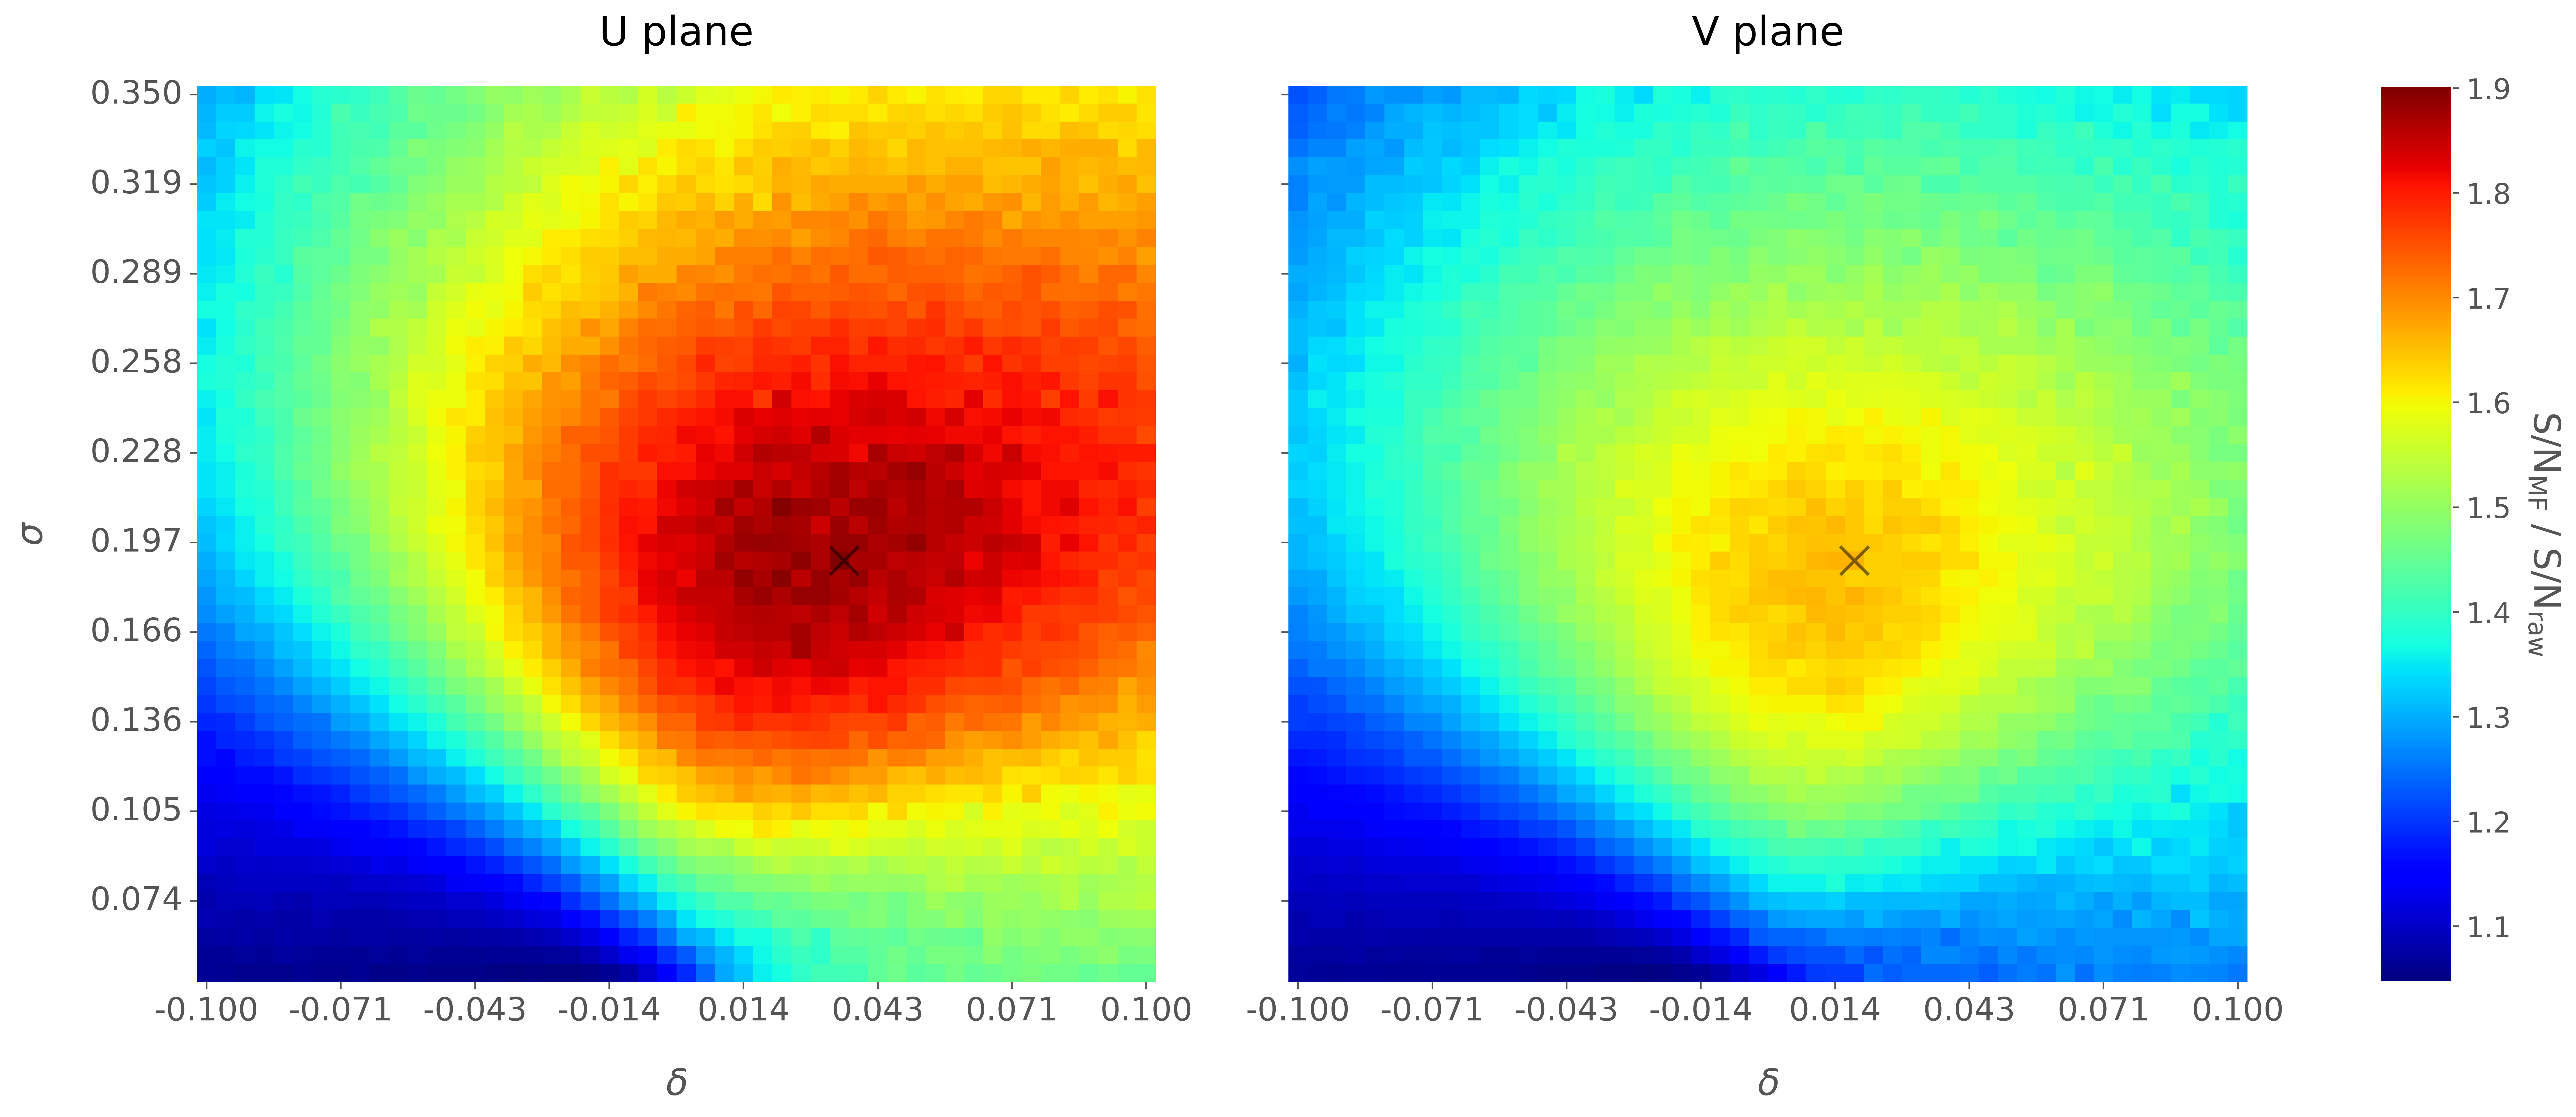
\includegraphics[width=1\linewidth]{Images/Matched_Filter/mf_fir_opt.png}
	\caption[Relative change in the S/N for the ProtoDUNE-SP raw data capture for different values of $\delta$ and $\sigma$ from the matched filter parametrisation.]{Relative change in the S/N for the ProtoDUNE-SP raw data capture \texttt{felix-2020-07-17-21:31:44} for different values of $\delta$ and $\sigma$ from the matched filter parametrisation in Eq. (\ref{2.4.13}). The black crosses in both panels denote the location of the maximum ratio value.}
	\label{fig:mf_opt}
\end{figure}

To test whether this choice of filter is appropriate one needs to choose a signal template. As an example of how a matched filter would affect our signal, I simply took the matched filter coefficients to be the 32 ADC values around a signal peak present in the data. In Fig. \ref{fig:adcs_mf} (left panel) I plotted a zoomed region for channel $7840$ in the raw data capture \texttt{felix-2020-07-17-21:31:44}, after applying the matched filter described before (blue line). When compared to the raw and FIR filtered case (see Figs. \ref{fig:adcs_nofir} and \ref{fig:adcs_fir}), after applying the matched filter the standard deviation of the noise waveform (red line) decreases and at the same time the signal peaks are enhanced. This leads to an improvement of the S/N by a factor of $1.92$ when compared to the raw waveform.

To obtain the matched filter that is more suitable for our data, I explored different configurations of signal templates. I parametrised the signal using the bipolar function:
\begin{equation}\label{2.4.13}
	f(x) = -A (x + \delta) \ \mathrm{e}^{-x^{2}/\sigma^{2}},
\end{equation}
where the parameter $\delta$ controls the asymmetry between the positive and negative peaks and $\sigma$ controls their width. The amplitude parameter $A$ is set such that it keeps the height of the biggest peak to be less than $200$ ADC in absolute value.

As this parametrisation is only adequate for bipolar signals I will focus exclusively on the induction channels. Also, to achieve the best possible performance, I optimise the coefficients for the U and V planes separately. However, as I will discuss, the differences are not very pronounced. In case it is not technically possible to separate channels in the firmware according to the plane they are coming from and use different sets of filter coefficients for them, we can just find a common set of coefficients. In such case, I do not expect the results to change drastically.

Figure \ref{fig:mf_opt} presents the results of the parameter scan, for channels in the induction planes U (left panel) and V (right panel). For each configuration of $\sigma$ and $\delta$ the resulting matched filter was applied to all channels in the corresponding plane within the data capture \texttt{felix-2020-07-17-21:31:44}. The change in S/N is computed with respect to the raw waveforms, and then the mean value for all channels is kept as a score for each filter. One can see that the improvements obtained for the U plane are in general higher than the ones for the V plane. However, these ratios are substantially higher than the ones obtained for the low-pass FIR filters. For the optimal configurations, I attained improvements up to a factor of $1.85$ for the U plane and $1.65$ for the V plane.

The sets of optimal matched filter coefficients were obtained for the parameters $\delta = 0.035$, $\sigma = 0.191$ for the U plane and $\delta = 0.018$, $\sigma = 0.191$ for the V plane. I show these two sets of coefficients in Fig. \ref{fig:mf_perf} (left panel). Figure \ref{fig:mf_perf} (right panel) shows the distribution of the S/N improvement after the optimal match filters for the U and V were applied to the corresponding channels in the raw data capture \texttt{felix-2020-07-17-21:31:44}. As mentioned before, the mean improvement achieved for the U plane channels is slightly higher than the one for the V channels. Note, however, that the spread of the distribution for the V plane is smaller than the one for the U plane.

Overall, one can see that the improvements on the S/N are much more significant in the case of the matched filter than they were for the low-pass FIR filters. The analysis of the raw data captures from ProtoDUNE-SP suggests that matched filters increase the S/N of induction channels by a factor of $1.5$ more than the optimal low-pass FIR filters.

Although these results are by themselves great points in favour of the matched filter, more studies are needed to completely assess the robustness of this approach. I proceeded then to test the matched filter with simulated data samples.

\begin{figure}[t]
	\begin{subfigure}{0.5\textwidth}
		\centering
		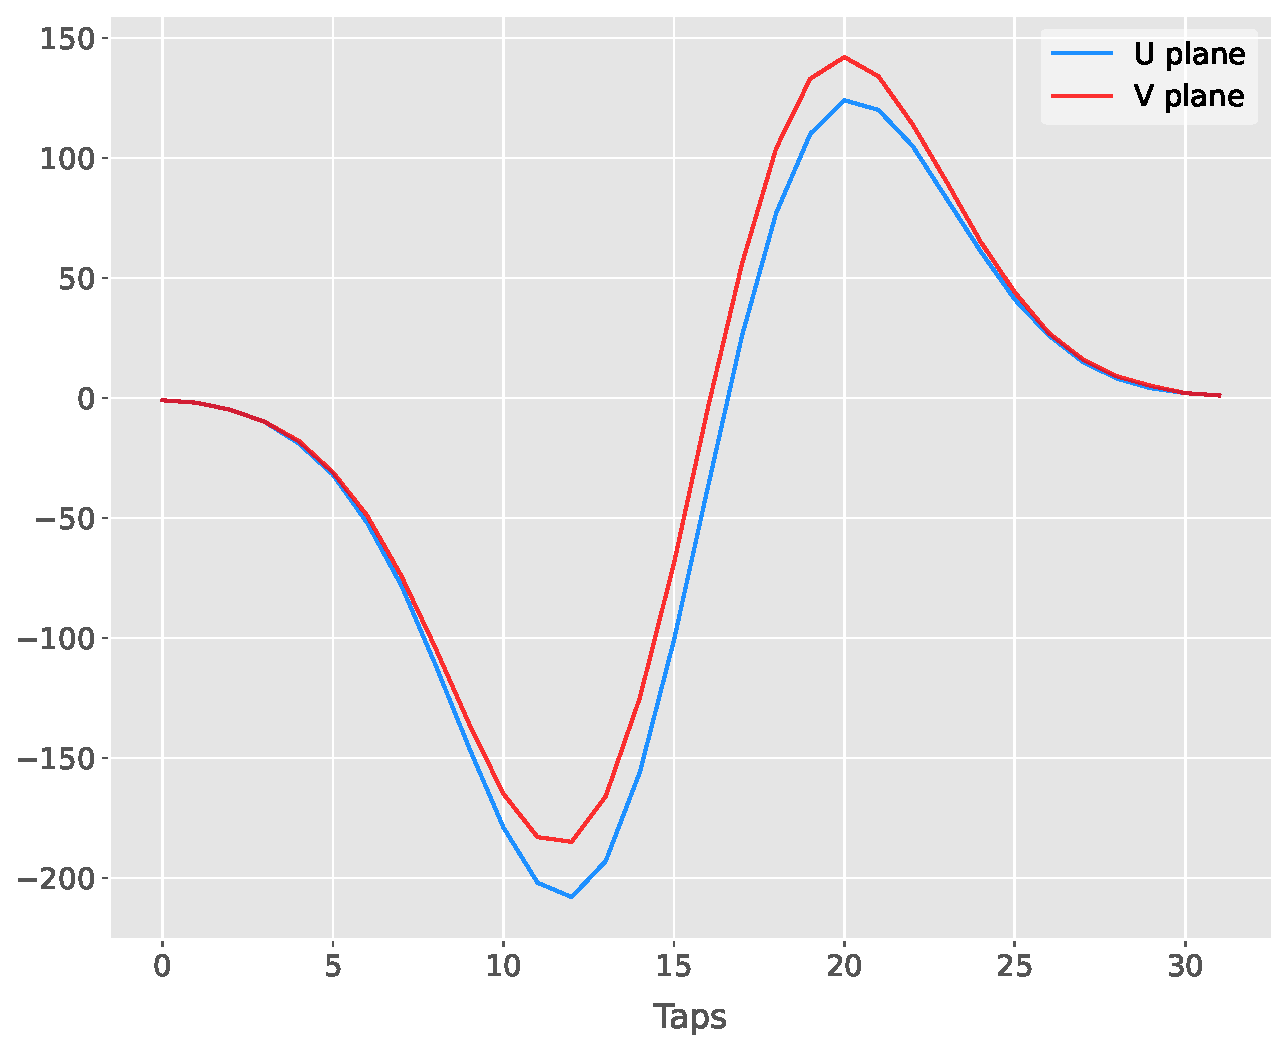
\includegraphics[width=.99\linewidth]{Images/Matched_Filter/optimal_coeffs}
	\end{subfigure}
	\begin{subfigure}{0.5\textwidth}
		\centering
		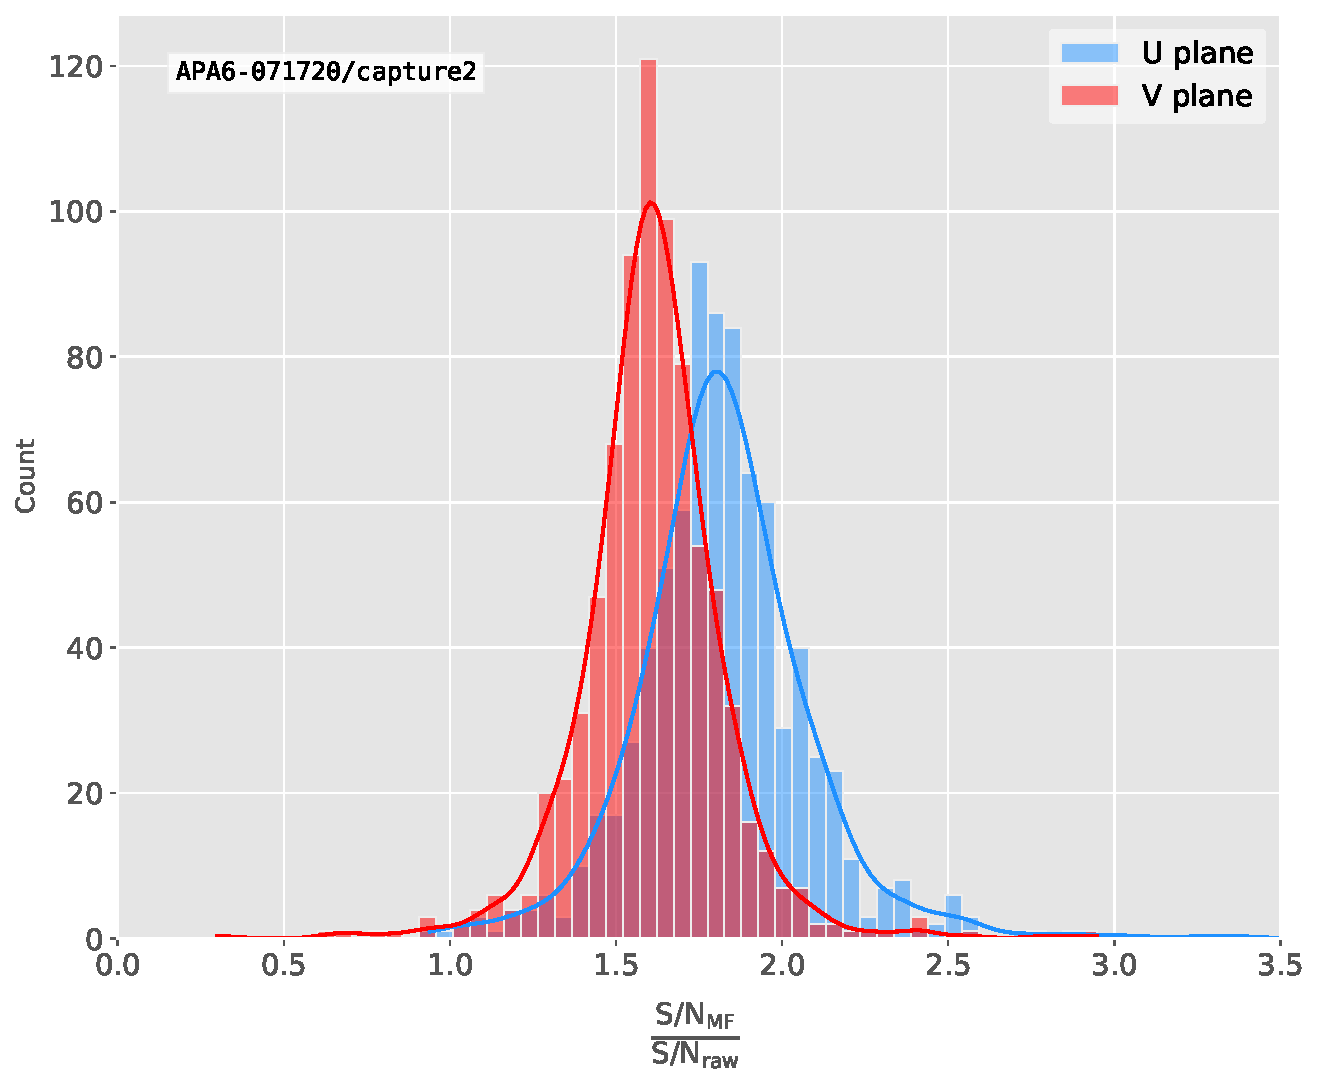
\includegraphics[width=.99\linewidth]{Images/Matched_Filter/improvement_capture}
	\end{subfigure}
	\caption[Distribution of the relative change of the S/N on the induction planes from the ProtoDUNE-SP raw data capture after their respective optimal matched filters were applied.]{Left panel: Optimal matched filter coefficients for the U (blue line) and V (red line) planes. The filters were computed with our parametrisation in Eq. (\ref{2.4.13}) for the parameter values $\delta = 0.035$, $\sigma = 0.191$ and $\delta = 0.018$, $\sigma = 0.191$ respectively. Right panel: Distribution of the relative change of the S/N on the two induction wire planes from the ProtoDUNE-SP raw data capture \texttt{felix-2020-07-17-21:31:44} after their respective optimal matched filters were applied.}
	\label{fig:mf_perf}
\end{figure}

\section{Monte Carlo studies}
\label{sec:matched_filter_mc_studies}

To further test the matched filter, the next step is to generate and process data samples using LArSoft \cite{Church2013}, the simulation and reconstruction software of the DUNE FD. In this way, one can control the particle content of the samples, the orientation of the tracks and their energy, and therefore see how the matched filter behaves in various situations.

To begin with, I prepared different monoenergetic and isotropic samples containing a single particle per event. Each sample contains a different particle species, namely electrons, muons, protons and neutral pions, all with a kinetic energy of $E_{k} = 100 \ \mathrm{MeV}$. I chose these because of the fairly different topologies they generate in the liquid argon, ranging from shower-like to track-like.

The event were generated with the single particle gun, and the Geant4 stage of the LArSoft simulation \cite{Church2013} was performed with the standard configuration for the DUNE FD HD design.

\begin{figure}[t]
	\begin{subfigure}{0.5\textwidth}
		\centering
		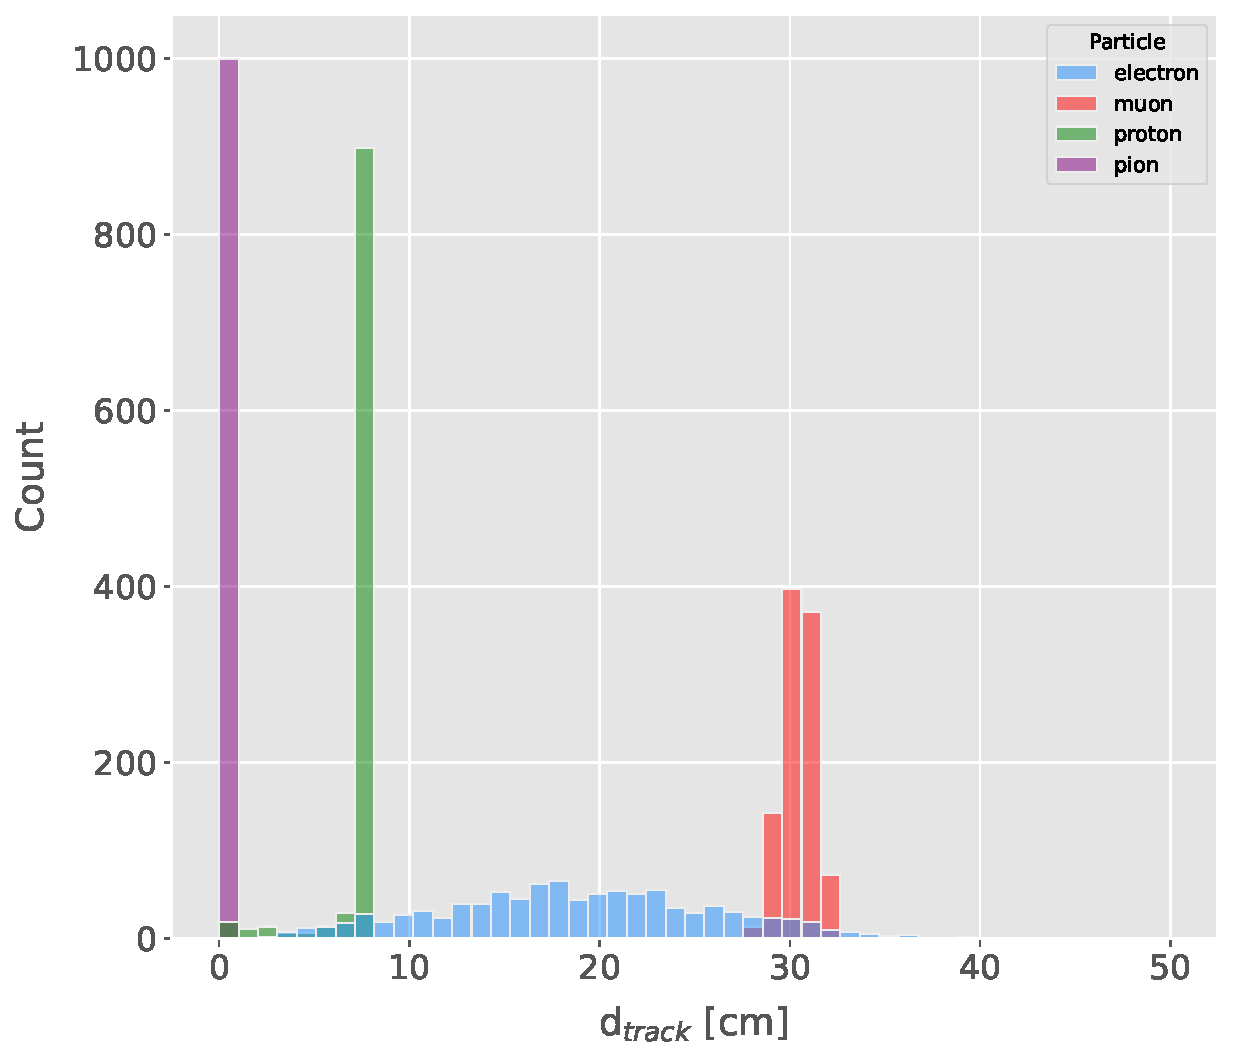
\includegraphics[width=.99\linewidth]{Images/Matched_Filter/particle_length}
	\end{subfigure}
	\begin{subfigure}{0.5\textwidth}
		\centering
		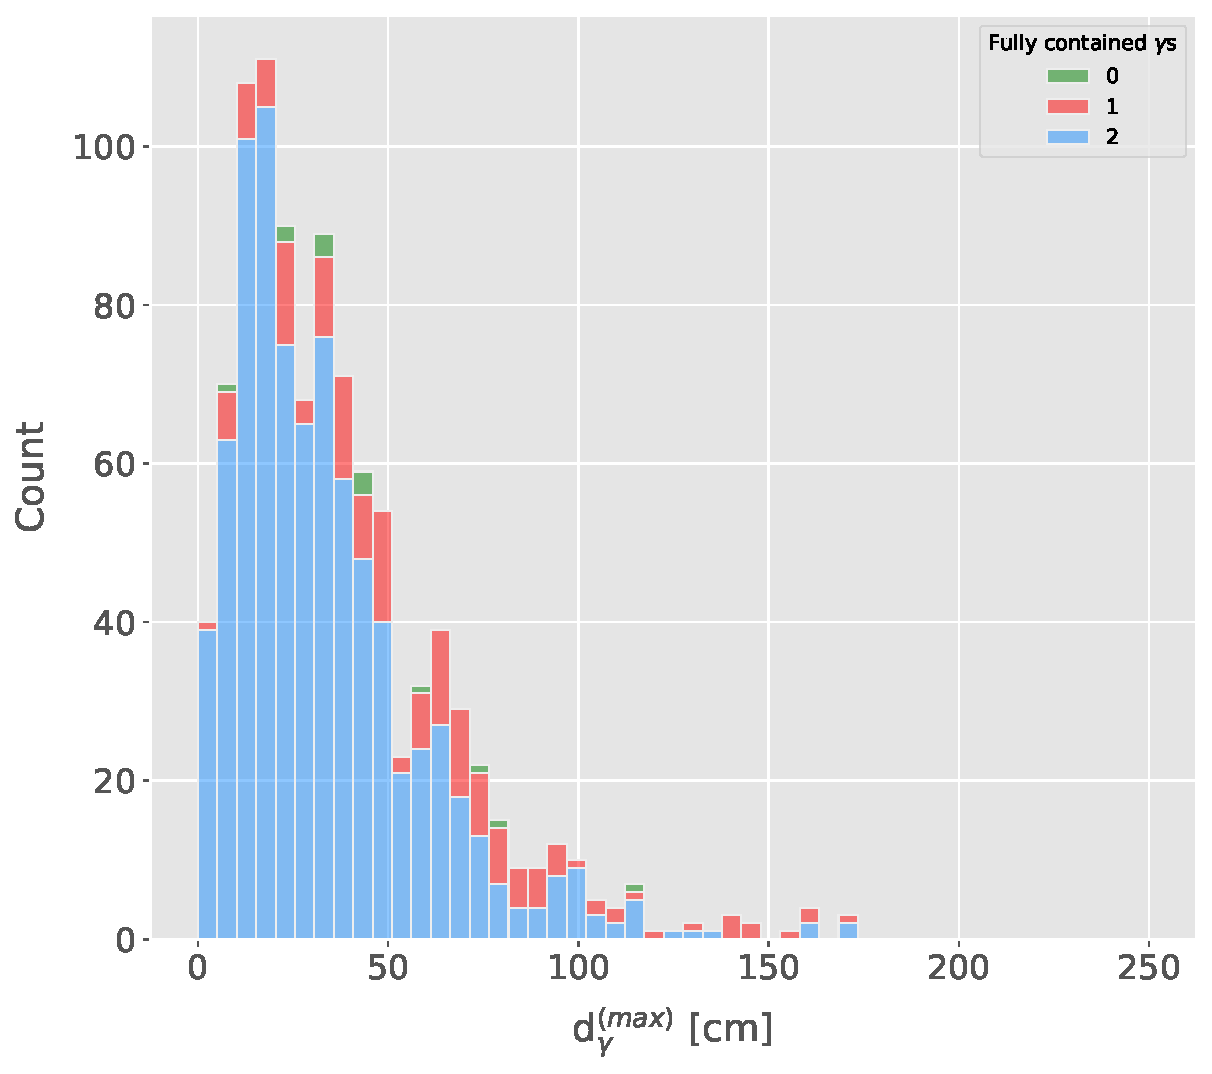
\includegraphics[width=.99\linewidth]{Images/Matched_Filter/gamma_length}
	\end{subfigure}
	\caption[Distributions of the particles track length in the liquid argon for the generated single particle monoenergetic samples.]{Left panel: distributions of the particles track length in the liquid argon for the generated $E_{k} = 100 \ \mathrm{MeV}$ monoenergetic samples, electrons (blue), muons (red), protons (green) and neutral pions (purple). Right panel: distribution of the length of the longest photon in the neutral pion sample after the decay process $\pi^{0} \rightarrow \gamma\gamma$.}
	\label{fig:lengths}
\end{figure}

For simplicity, I restricted the particles to start drifting in a single TPC volume\footnote{A TPC volume is defined as the drift region between a single APA and the cathode. Therefore, for one drift volume of a HD module, there are twice as many TPC volumes as there are APAs in the corresponding anode.}, so I can focus exclusively on the signals coming from one APA. The chosen kinetic energy for all the particles is $E_{k} = 100 \ \mathrm{MeV}$, as this produce tracks which are typically contained in one TPC volume. Figure \ref{fig:lengths} (left panel) shows the distributions of the track lengths in the liquid argon of all generated particles with $E_{k} = 100 \ \mathrm{MeV}$. One can see that, in the case of the track-like particles (i.e. muons and protons), their length distributions are quite sharp and centered at relatively low distances ($30$ and $8 \ \mathrm{cm}$, respectively). For electrons, the distribution is quite broad but it does not extend past $\sim 30 \ \mathrm{cm}$. The case of the neutral pions can be misleading. As they decay promptly, the track length associated to the true MC particle is always $< 1 \ \mathrm{cm}$. In Fig. \ref{fig:lengths} (right panel) I show the effective length distribution of the longest photon after the pion decays as $\pi^{0} \rightarrow \gamma \gamma$, highlighting the number of fully contained photons in the TPC volume per event (either zero, one, or two). One can see that the vast majority of events have both photons contained in the TPC volume, whereas just a negligible fraction of them have none. However, for the sake of caution, I keep only the pion events with both photons contained.

The next step is to process the sample through the detector simulation. To make adequate estimations of the noise levels, one needs to turn off the default zero-suppression of the waveforms produced by the simulation. At this stage I am only interested int the waveforms with noise added, so I keep the noise addition option as true in the configuration. However, for studies related to the hit finder performance one also needs to store the noiseless waveforms, to retrieve the truth information of the hits. I will discuss this approach next.

To reduce the amount of data that will go for processing, I used the information from the Geant4 step of the simulation to select only the active channels, i.e. the channels where some ionisation electrons arrived. Moreover, I only extract the waveforms from one APA and exclusively the ones coming from induction channels. The resulting \texttt{ROOT} file contains a \texttt{TTree} with two branches, one containing the waveforms for each event and channel and the other with the corresponding offline channel numbers.

Finally, I extract the truth values for the orientation of the tracks and the energies of the particles to use them in the analysis. These are stored in a \texttt{ROOT} file with a single \texttt{TTree}, containing several branches with information such as the components of the initial momentum of the particles, initial and final positions, track length, etc.

For the analysis of the resulting waveforms and truth values I used a custom analysis code independent of LArSoft. Among other functionality, it allows the user to read the \texttt{ROOT} files, export the raw data as \texttt{pandas} objects, apply the filters and compute the S/N of both the raw and filtered signals. The default configuration for the filtering uses the set of optimal matched filter coefficients that I found using the ProtoDUNE-SP data samples.

\begin{figure}[t]
	\begin{subfigure}{0.5\textwidth}
		\centering
		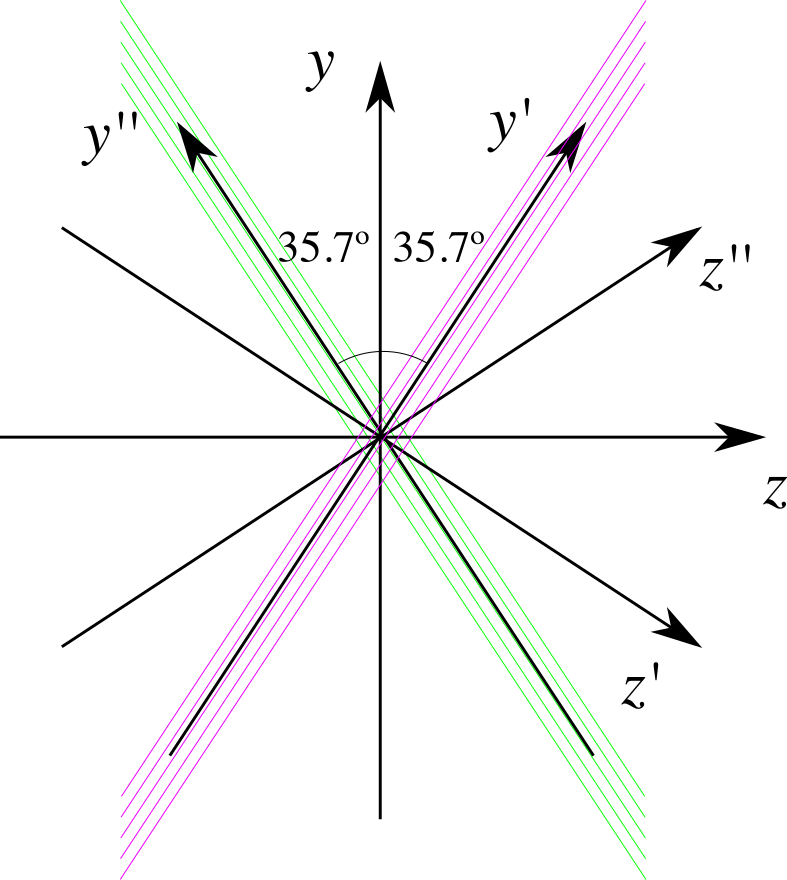
\includegraphics[width=.8\linewidth]{Images/Matched_Filter/sim_rotation}
	\end{subfigure}
	\begin{subfigure}{0.5\textwidth}
		\centering
		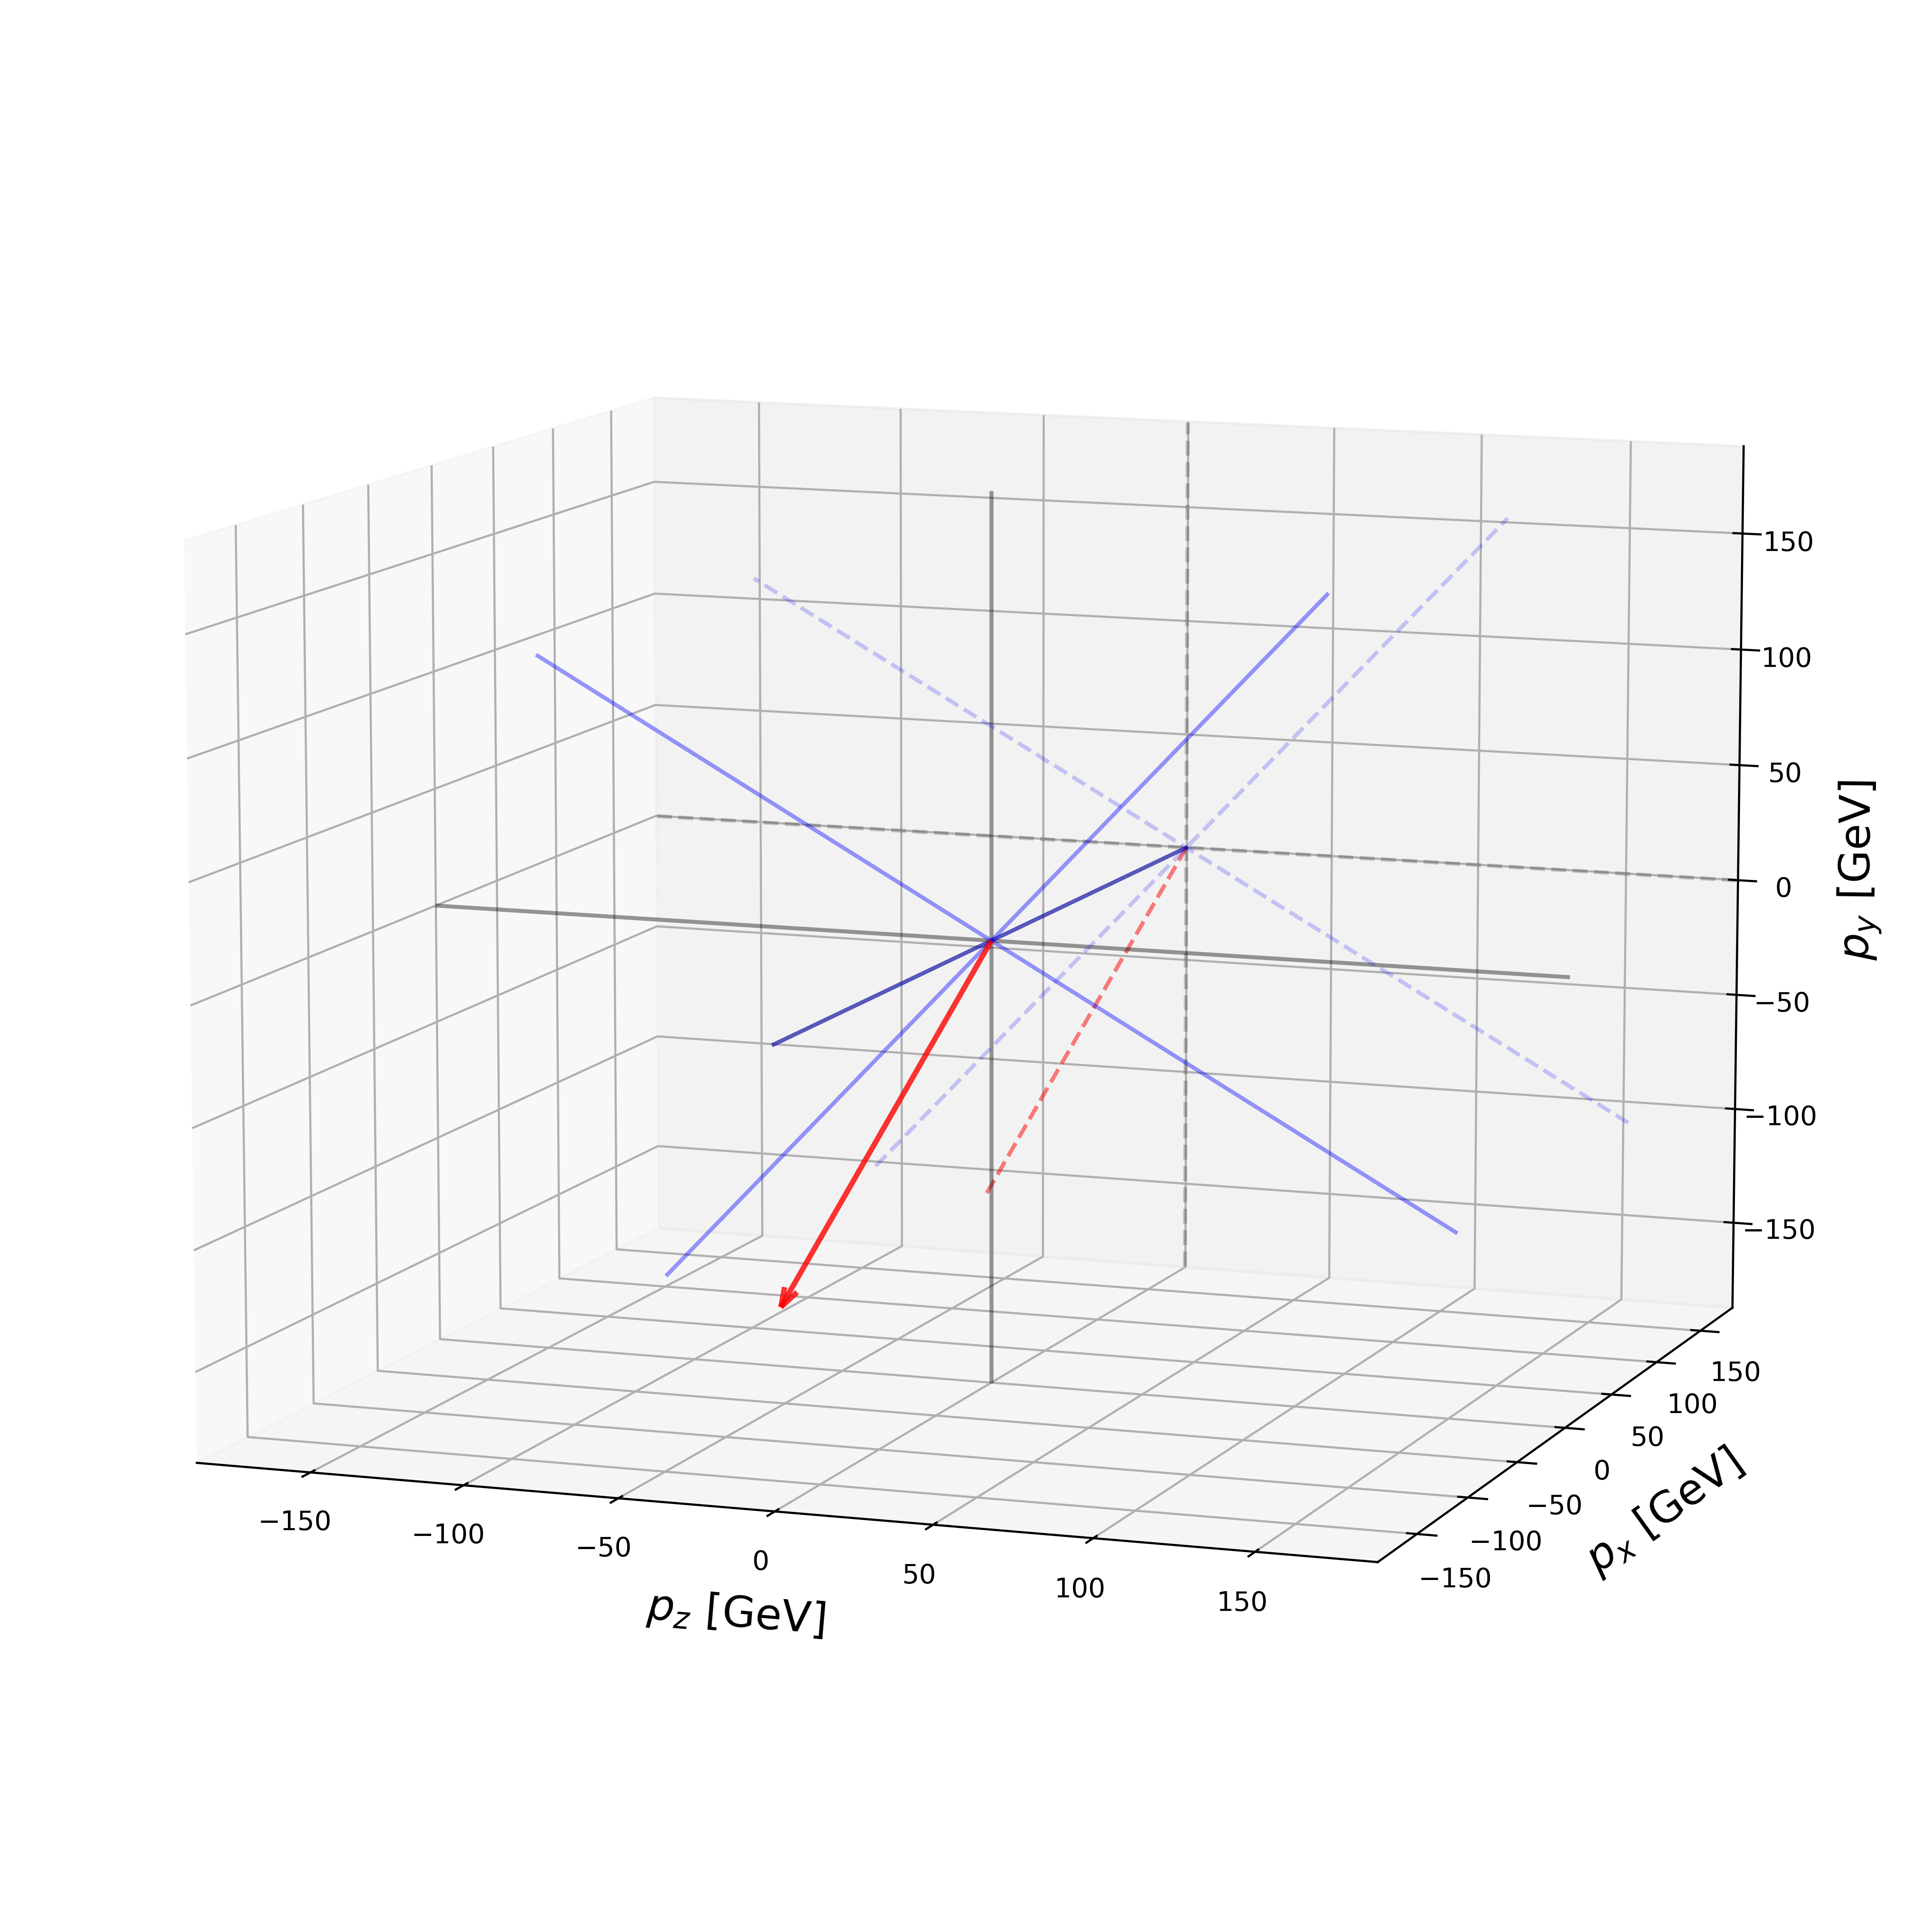
\includegraphics[width=.99\linewidth]{Images/Matched_Filter/3D_rotation}
	\end{subfigure}
	\caption[Schematic representation of the two rotated reference frames used in the analysis of the MC filter performance.]{Left panel: schematic representation of the two new rotated reference frames used in this analysis (denoted as prime and double prime), viewed from the $yz$ plane. The magenta stack of lines represent the wires in the U plane, whereas the green lines correspond to the wires in the V plane. Right panel: 3D representation of the momentum of one of the generated monoenergetic muons (red arrow) in the original reference frame (black lines), along with the new reference frame used for the U plane waveforms (blue lines). In the $yz$ plane I added the projection of these three.}
	\label{fig:reference_frame}
\end{figure}

Additionally, for the analysis of the samples it was necessary to use two different reference frames, to study separately the signals coming from the U and V induction planes. Focussing on a single APA, the U and V channels have a different orientation in the $yz$ plane. In the case of U channels, these are tilted $35.7^{\circ}$ clockwise from the vertical ($y$ direction), whereas the V channels are at the same angle but in the counter-clockwise direction. Because of this, the best option is to deal with two new coordinate systems rotated by $\pm 35.7^{\circ}$ along the $x$ axis, so the new $y'$ and $y''$ directions are aligned with the U and V induction channels, respectively. Figure \ref{fig:reference_frame} (left panel) shows a schematic representation of the original reference frame together with the two rotated ones (denoted by primed and double primed). This way, one can easily understand how parallel was a track to the channels in the two induction planes. Figure \ref{fig:reference_frame} (right panel) shows a 3D representation of the momentum of a track (red arrow) in the original reference frame (black lines), along with the new reference frame for the U plane (blue lines). I added the projections onto the $yz$ plane of these, to show the usefulness of the new reference frame to tell whether a track is parallel or perpendicular to the channels in a induction plane.

\begin{figure}[t]
	\centering
	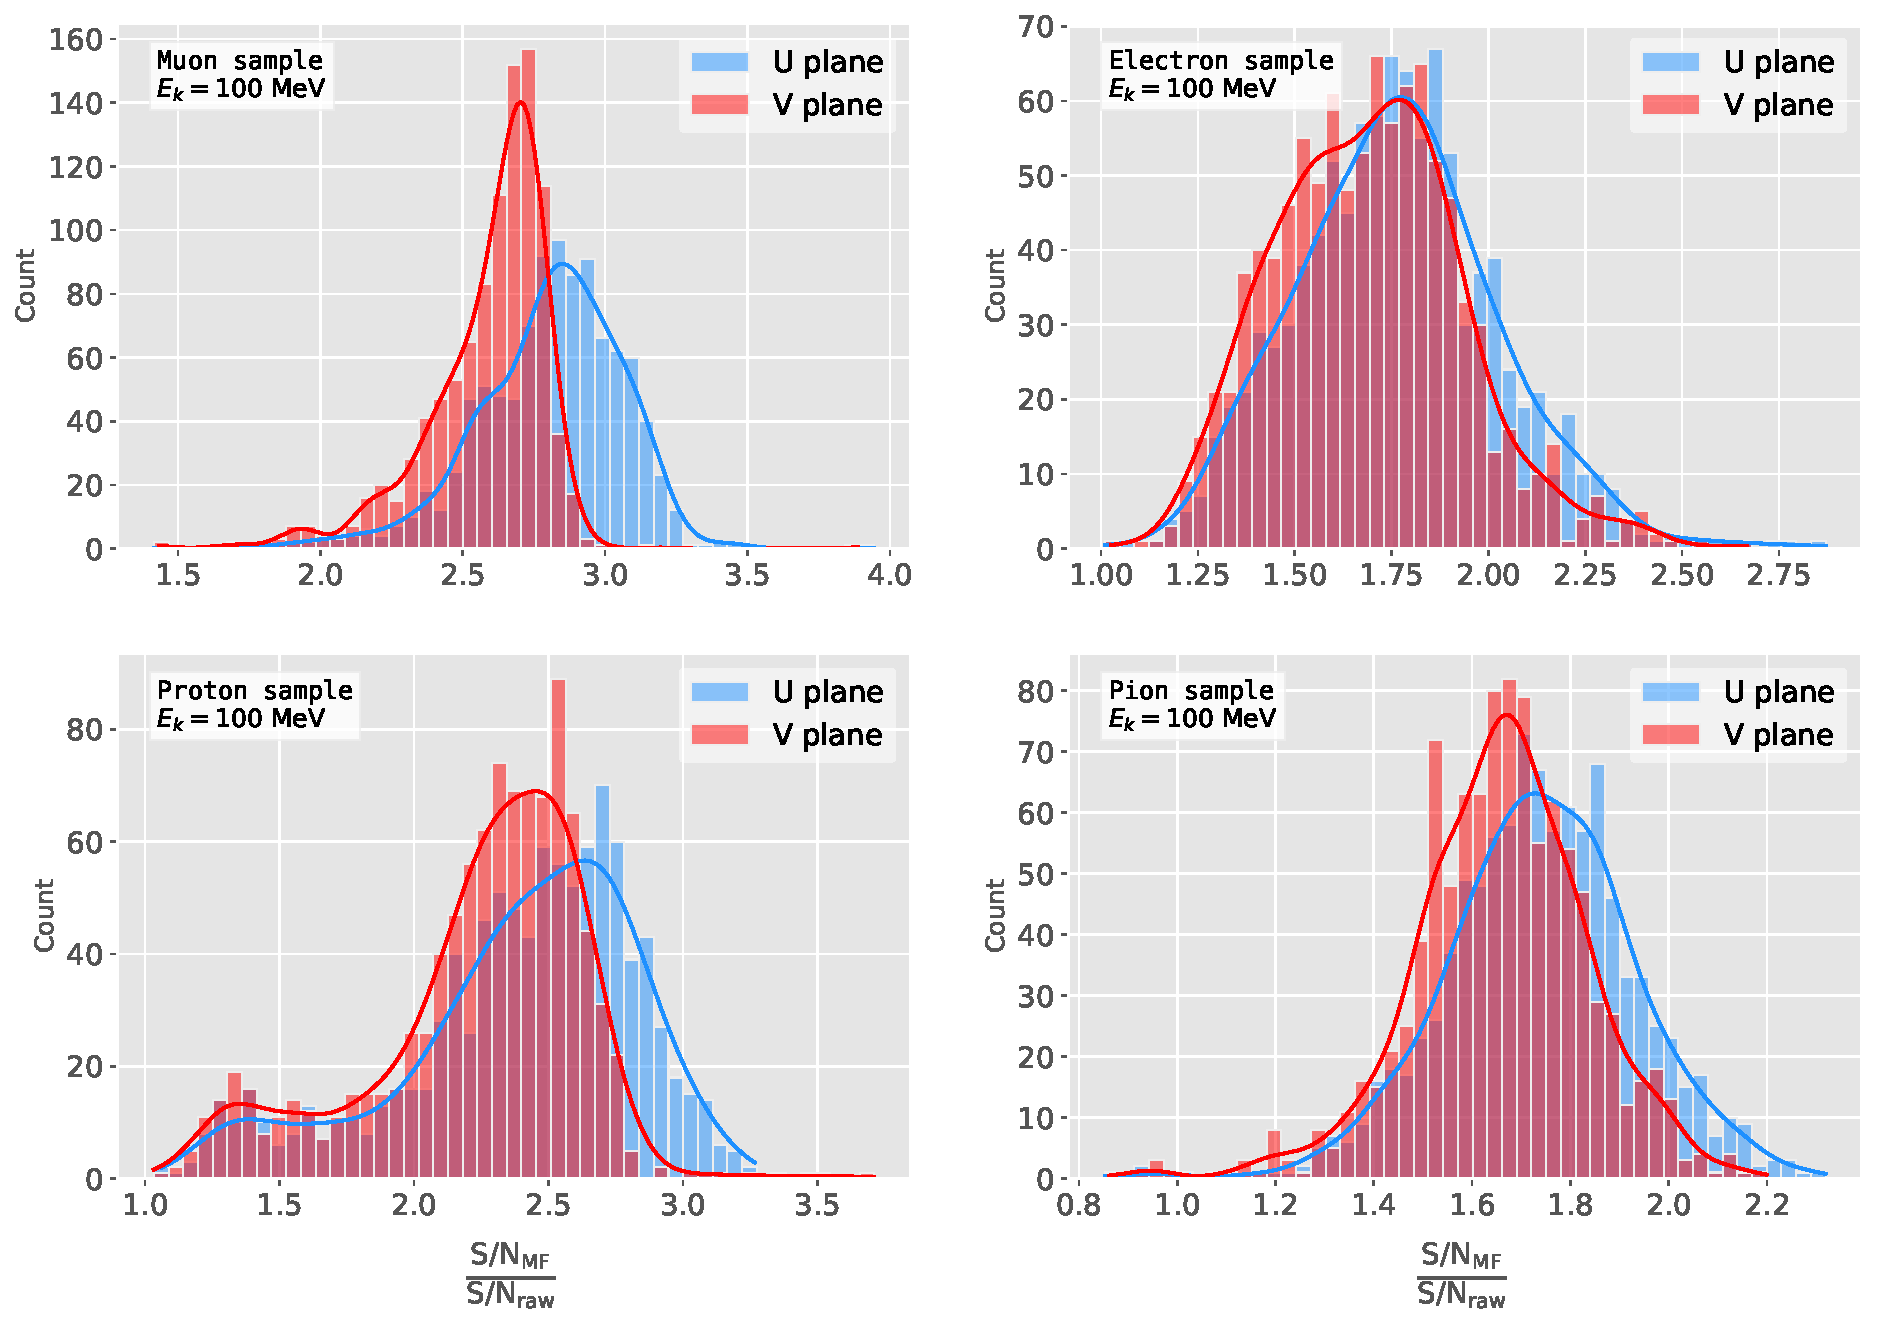
\includegraphics[width=0.9\linewidth]{Images/Matched_Filter/larsoft_sn_hists.pdf}
	\caption[Distributions of the mean S/N change per event for the different MC samples after applying the matched filters.]{Distributions of the mean S/N change per event for the different MC samples after applying the matched filters. Here I separated the change in the U plane (blue) and the V plane (red) channels. From top left to the right: muon, electron, proton and neutral pion. All the events have a fixed kinetic energy of $E_{k} = 100 \ \mathrm{MeV}$.}
	\label{fig:mono_summary_hist}
\end{figure}

Figure \ref{fig:mono_summary_hist} shows the distribution of the average S/N change per event when I apply the optimised matched filters. I produce separate distributions for the channels in the U (red) and V (blue) induction planes. Notice that the S/N distributions for the track-like particles, i.e. muons (top left panel) and protons (bottom left panel), have significantly larger mean values than the distributions of the shower like particles, i.e. electrons (top right panel) and neutral pions (bottom right panel). An important difference between these results and the ones obtained before for the ProtoDUNE-SP data is that the overall improvements that I get with simulated data are more significant. This could be due to an underestimation of the noise levels in the LArSoft simulation. Nonetheless, the concluding message is that the previously optimised matched filters give an overall significant improvement of the S/N for the different samples.

About the convention I follow to present the results results, in the case of the raw and filtered S/N of each event I take the average of these quantities over all the active channels in the event. That is, if a certain event has $N_{chan}$ active channels the two S/N values are computed as:
\begin{equation}
\begin{split}
\left(S/N_{fir}\right)_{event} &= \frac{\sum_{i=0}^{N_{chan}} \left(S/N_{fir}\right)_{i}}{N_{chan}},\\
\left(S/N_{raw}\right)_{event} &= \frac{\sum_{i=0}^{N_{chan}} \left(S/N_{raw}\right)_{i}}{N_{chan}}.
\end{split}
\end{equation}
However, for the ratio of the raw and filtered S/N (what I call the S/N change) per event I do not take the ratio of the previous two quantities but compute the average of the individual ratios per channel in the event:
\begin{equation}
\left(\frac{S/N_{fir}}{S/N_{raw}}\right)_{event} = \frac{\sum_{i=0}^{N_{chan}} \left(\frac{S/N_{fir}}{S/N_{raw}}\right)_{i}}{N_{chan}},
\end{equation}
therefore:
\begin{equation}
\left(\frac{S/N_{fir}}{S/N_{raw}}\right)_{event}  \neq \frac{\left(S/N_{fir}\right)_{event}}{\left(S/N_{raw}\right)_{event}}.
\end{equation}

\subsection{Angular dependence}
\label{subsec:2.5.1}

\begin{figure}[t]
	\centering
	\includegraphics[width=0.9\linewidth]{Images/Matched_Filter/larsoft_muon_angular.pdf}
	\caption[Angular dependence of the mean S/N and the S/N improvement for the monoenergetic muon sample.]{Angular dependence of the mean S/N and the S/N improvement for the monoenergetic muon sample. The top and bottom rows correspond to the U and V planes, respectively. The top subplots show the mean S/N for raw (blue) and filtered (red) waveforms whereas the bottom subplots depict the averaged S/N improvement (black).}
	\label{fig:angular_muon}
\end{figure}

Having these monoenergetic samples, one can study the angular dependence of the matched filter performance. This is an important point, as it is a well established fact that for certain track configurations the S/N is much lower than average as the corresponding waveforms are severely distorted. Therefore, I am interested in seeing how the matched filter behaves in different cases and how the S/N change for those compare to the average.

\begin{figure}[t]
	\centering
	\includegraphics[width=0.9\linewidth]{Images/Matched_Filter/larsoft_electron_angular.pdf}
	\caption[Angular dependence of the mean S/N and the S/N improvement for the monoenergetic electron sample.]{Angular dependence of the mean S/N and the S/N improvement for the monoenergetic electron sample. The top and bottom rows correspond to the U and V planes, respectively. The top subplots show the mean S/N for raw (blue) and filtered (red) waveforms whereas the bottom subplots depict the averaged S/N improvement (black).}
	\label{fig:angular_electron}
\end{figure}

Figure \ref{fig:angular_muon} shows the angular dependence of the S/N for the monoenergetic $E_{k}=100 \ \mathrm{MeV}$ isotropic muons, for the different induction planes and projections. The angles for each event are given by the components of the initial value of the momentum of the particles, taking the angles of the projections on the $xz$ and $yz$ planes with respect to the $z$ axis (more accurately, one needs to compute these angles twice for each event, a pair for the $xy'z'$ coordinate system and the other for the $xy''z''$, as explained previously). The top row shows the dependence on the angles corresponding to the U plane, i.e. $\theta_{xz'}$ and $\theta_{y'z'}$, whereas the bottom row shows the angular dependence viewed from the V plane, $\theta_{xz''}$ and $\theta_{y''z''}$. In each panel, the top subplot represents the mean values of the S/N for the raw (blue) and matched filtered (red) signals, and the bottom subplot the averaged S/N change (black). The solid lines represent the mean value obtained for the corresponding angular bin, whereas the semitransparent bands represent one standard deviation around the mean at each point.

As expected, the S/N is in general higher when tracks are parallel to the APA (i.e. $\theta_{xz} \sim 0$) and lower when they are normal to the plane ($\theta_{xz} \sim \pm 90^{\circ}$). In the same way, tracks parallel to the wires ($\theta_{yz} \sim \pm 90^{\circ}$) tend to have higher S/N than those perpendicular to these ($\theta_{yz} \sim \pm 0$).

Figure \ref{fig:angular_electron} shows the corresponding angular dependence results for the $E_{k}=100 \ \mathrm{MeV}$ electrons sample. Notice that, in this case, the S/N behaviour discussed above does not hold. A possible explanation can be that, because most hits in these events are produced by the secondary particles generated in the EM shower, the signal peaks whose S/N ratios were computed do not correspond to the directional information of the primary electron.

\begin{figure}[t]
	\begin{subfigure}{0.5\textwidth}
		\centering
		\includegraphics[width=.99\linewidth]{Images/Matched_Filter/evt_xz_0_yz_90_U}
	\end{subfigure}
	\begin{subfigure}{0.5\textwidth}
		\centering
		\includegraphics[width=.99\linewidth]{Images/Matched_Filter/evt_xz_90_yz_0_U}
	\end{subfigure}
	\caption[Waveforms for two muon events, one parallel to the APA and to the wires in the U plane and other normal to the APA plane and perpendicular to the U plane wires.]{Selected consecutive waveforms corresponding to two monoenergetic $E_{k} = 100 \ \mathrm{MeV}$ muon events, one is parallel to the APA and to the wires in the U plane (left panel) and the other is normal to the APA plane and perpendicular to the U plane wires (right panel). The solid lines represent the raw waveforms whereas the dashed lines correspond to the waveforms after the matched filter was applied. The waveforms on the left panel have been scaled by a factor of $0.15$ to have similar amplitudes to the ones on the right panel.}
	\label{fig:example_orientation}
\end{figure}

\subsection{Distortion and peak asymmetry}
\label{sec:A.5}

As a case study, I select two of the simulated $E_{k} = 100 \ \mathrm{MeV}$ monoenergetic muon events. With respect to the U induction plane, one is parallel to the APA (low $\theta_{xz'}$) and to the wires (high $\theta_{y'z'}$) and the other is normal to the APA plane (high $\theta_{xz'}$) and perpendicular to the wires (low $\theta_{y'z'}$). As expected from the results on the angular dependence discussed above, the former has a higher S/N (both before and after the filtering) when compared to the latter. An interesting thing to notice about these two samples is that, even though one has a much larger S/N than the other, it is the one with the smallest S/N the one that gets a more significant averaged S/N improvement. In Tab. \ref{tab:case} I include all the relevant parameters of these two $E_{k} = 100 \ \mathrm{MeV}$ muon events, namely the angles with respect to the $xy'z'$ reference frame, the values of the S/N, the S/N change and also the so-called peak asymmetry $\Delta_{peak}$, that I will define next.

\begin{figure}[t]
	\begin{subfigure}{0.5\textwidth}
		\centering
		\includegraphics[width=.99\linewidth]{Images/Matched_Filter/deltaPeak_dist}
	\end{subfigure}
	\begin{subfigure}{0.5\textwidth}
		\centering
		\includegraphics[width=.99\linewidth]{Images/Matched_Filter/deltaPeak_SN_ratio}
	\end{subfigure}
	\caption[Distribution of the peak asymmetry for the monoenergetic muon sample and dependence of the S/N change on the mean peak asymmetry of the event.]{Left panel: peak asymmetry distribution for the case of the monoenergetic $E_{k} = 100 \ \mathrm{MeV}$ muon sample. Each value corresponds to a single bipolar signal peak from a channel in any event. The blue distribution represents the peaks on U plane channels, whereas the red corresponds to signal peaks in V wires. Right panel: relation between the mean peak asymmetry per event with the S/N for U channel waveforms from the $E_{k} = 100 \ \mathrm{MeV}$ muon sample. The top subplot shows the decimal logarithm of the mean S/N for the raw (red) and the matched filtered (blue) waveforms. The bottom subplot contains the mean S/N improvement ratio after the matched filter was applied.}
	\label{fig:asymmetry}
\end{figure}

\begin{table}[h!]
	\centering
	\caption[Characteristic parameters of the two monoenergetic muon events selected for the peak asymmetry study.]{Characteristic parameters of the two monoenergetic muon events selected, relative to the U plane: projected angles in the $xz'$ and $y'z'$ planes, S/N values for the raw and filtered waveforms, mean improvement of the S/N and peak asymmetry.}
	\begin{tabular}{l|llllll}
		& $\theta_{xz'} \ (^{\circ})$ & $\theta_{y'z'} \ (^{\circ})$ & $\mathrm{S/N}_{\mathrm{raw}}$ & $\mathrm{S/N}_{\mathrm{MF}}$ & $\frac{\mathrm{S/N}_{\mathrm{MF}}}{\mathrm{S/N}_{\mathrm{raw}}}$ & $\Delta_{peak} \ (\mathrm{ADC})$ \\ \hline
		High ("parallel") & -1.58                     & -77.76                     & 41.65       & 112.44      & 2.83                          & -35.73                                                          \\
		Low ("normal")  & 76.92                     & -2.56                      & 8.07        & 25.46       & 3.12                          & -10.38                                                         
	\end{tabular}
	\label{tab:case}
\end{table}

One can try to understand better the nature of these two events by looking at the raw and filtered data from some of their active channels. Figure \ref{fig:example_orientation} shows a selection of consecutive raw and filtered U plane waveforms from the event with high S/N (left panel) and the one with low S/N (right panel). To show both collections of waveforms at a similar scale I had to apply a factor of $0.15$ to the waveforms with high S/N. Additionally, next to each waveform I include the values of the raw and matched filtered S/N for the corresponding channel. The first thing to notice is that the amplitude of the signal peaks from the normal track have a much smaller amplitude, and also appear quite distorted when compared to the others. On the other hand, although the matched filtered S/N for each channel are still smaller, the relative improvements are larger than in the parallel case.

A way to quantify the difference between the shape of the waveforms of these two events is using their peak asymmetry. I define the peak asymmetry as the (signed) difference between the positive and the negative peaks of the bipolar shape, i.e.:
\begin{equation}
\Delta_{peak} \equiv h_{+} - h_{-},
\end{equation}
where both heights $h_{+}$ and $h_{-}$ are positive. Figure \ref{fig:asymmetry} (left panel) shows the distribution of this peak asymmetry for all the waveforms corresponding to channels in the U (blue) and V (red) planes for the monoenergetic muon sample. One can see that these distributions are clearly shifted to negative values, with means $\mu_{\Delta}^{\mathrm{U}} = -10.57 \ \mathrm{ADC}$ and $\mu_{\Delta}^{\mathrm{V}} = -5.72 \ \mathrm{ADC}$, respectively. Notice how the peak asymmetry value of the selected event with the high S/N sits at the left tail of the distribution, whereas the corresponding value of the sample with the low S/N lies around the mean.

It is possible to correlate the peak asymmetry with the S/N and the S/N change per event. Figure \ref{fig:asymmetry} (right panel) shows the result of comparing the mean peak asymmetry per event to the averaged raw (red) and matched filtered (blue) S/N per event (top subplot). The horizontal lines sit at the mean value obtained in the fit and represent the width of the $-\Delta_{peak}$ bins used, while the vertical lines indicate one standard deviation around that mean value. Notice how there is an approximate linear relation between the peak asymmetry and the S/N, except for peak asymmetry values bigger than $- 5 \ \mathrm{ADC}$ where the S/N remains constant.

Also, in the bottom subplot of Fig. \ref{fig:asymmetry} (right panel) I show the relation between the peak asymmetry and the mean S/N change. In this case, one can see that there is a clear maximum at $\Delta_{peak} \sim -10 \ \mathrm{ADC}$. As mentioned previously, this is also the value of the mean of the peak asymmetry distribution. In fact, it is expected that our filter favours the signal peaks with the most common values of the peak asymmetry, as this was one of the features I target in our filter coefficient optimisation through the parameter $\delta$.

These results suggest that events with poorer values of the mean S/N, usually associated to non-favourable track orientations, tend to have smaller values of the mean peak asymmetry (in absolute value). Nonetheless, because our matched filters have been optimised to account for these asymmetries, the improvement on the S/N for these events is sizeable if not better than the one for events which already had a high S/N.

\subsection{Hit sensitivity}
\label{subsec:2.5.3}

\begin{figure}
	\centering
	\includegraphics[width=0.9\linewidth]{Images/Matched_Filter/electron_k100_full_run_1_evt_3}
	\caption[Raw event display for an electron event showing the true, standard, and matched filter hits produced.]{Raw event display showing the time (in firmware ticks) versus offline channel number for a $E_{k} = 100 \ \mathrm{MeV}$ electron event. The produced true hits are superimposed (black boxes) as well as the hits coming from the standard hit finder chain (blue circles) and the hit finder using the matched filter (green triangles).}
	\label{fig:evthitcomp}
\end{figure}

One of the advantages of the matched filter, directly related to increasing the S/N, is the capability of forming TPs that before fell below the threshold. For instance, Fig. \ref{fig:evthitcomp} shows the raw ADC data from an example electron event with the produced true hits superimposed (black boxes), together with the hits produced by the standard hit finder chain (blue circles), i.e. using the current FIR filter, and the hits obtained using the matched filters (green triangles). Both the standard and the matched filter hit finders run with a threshold of $10 \ \mathrm{ADC}$. Notice that the standard hits match well the true ones in the initial part of the event, where we have a track-like object. However, it misses most of the hits produced by the EM shower at later times. On the other hand, the hits produced with the matched filter have a better agreement with the true hits even for the more diffuse shower activity.

Even though the matched filter produces more hits as a results of the enhancement of the signal peaks relative to the noise level, it is also true that it may pick up some spurious hits not related to any real activity if one lowers the thresholds too much. Therefore, some optimisation of the threshold is needed, as there is a trade-off between precision and sensitivity.

Having this in mind, I compare the produced hits from both the standard  and the matched filter hit finders to the true hits. By running the hit finders on the samples with different values of the threshold I can understand how low these can be pushed, and then evaluate the gains obtained from this.

To study how the hit formation depends on the energy, I prepared new isotropic samples with the same types of particles as previously (muons, electrons, protons and neutral pions) but with a flat kinetic energy distribution ranging from $5$ to $100 \ \mathrm{MeV}$.

To estimate the hit sensitivity for a certain sample, one needs to recover the set of true hits to be able to compare these with the ones produced. To do so, I modify the procedure I use to extract the raw waveforms. For this kind of study, I run the detector simulation in two steps, first I produce the waveforms without noise and extract them in the same format I used for the raw data. Then, the noise is added and the noisy waveforms are similarly written to a file.

To have a better comparison between the true hits and the ones produced from the raw waveforms after applying the two filters, I apply the FIR filter and the matched filters to the noiseless waveforms as well. I run the hit finder with a minimal threshold (in this case I use $1 \ \mathrm{ADC}$) on the filtered noiseless waveforms, generating two sets of true hits. I will refer to these as the standard true hits (with the default FIR filter) and the matched filter true hits, respectively. This allows for a more precise matching between the different groups of hits produced, as it will account for any delays and distortions introduced by the filters.

In the case of the raw waveforms (with noise added), I run the hit finder on them with different values of the threshold, after applying either the FIR or the matched filters. I name theses simply standard and matched filter hits, respectively. Then, I match the generated hits to the true hits, the standard hits to the standard true hits and the matched filter hits to the matched filter true hits. The matching is performed by comparing the channel number and the timestamp of the hits. To count as a match, I require that all hits with the same channel number and timestamp have overlapping hit windows, i.e. the time windows between their hit end and hit start times need to overlap. If more than one hit in one of the groups have hit overlap with the same hit in the other group, I only count the match with the closest hit peak time value.

To quantify the performance of the two hit finder approaches, I use a classical method from statistical classification known as confusion matrix \cite{Stehman1997}. It divides the outputs in four categories: true positive (TP, both truth and predicted values are true), false negative (FN, truth value is true but predicted is false), false positive (FP, truth value is false but predicted is true) and true negative (TN, both truth and predicted values are false).

\begin{figure}[t]
	\centering
	\includegraphics[width=.99\linewidth]{Images/Matched_Filter/hit_study_muon_scores_indct}
	\caption[Dependence of the precision, sensitivity, and $F_{1}$ scores on the threshold values used in the hit finder for the FIR and matched filters.]{Dependence of the precision (blue), sensitivity (red), and $F_{1}$ (green) scores on the threshold values used in the hit finder, for the FIR (left panel) and matched filter (right panel) cases. The results were obtained after matching the hits to the true hits in the case of the isotropic muon sample with kinetic energy in the range $5$ to $100 \ \mathrm{MeV}$, taking only into account the induction plane channels. The points represent the mean value while the error bars indicate one standard deviation around that mean value.}
	\label{fig:threshold_opt}
\end{figure}

The contents of the confusion matrix allow us to compute other derived scores to assess the performance of our classification. In this study, I make use of three of these metrics, namely the precision or positive predictive value:
\begin{equation}
	\mathrm{PPV} = \frac{\mathrm{TP}}{\mathrm{TP} + \mathrm{FP}},
\end{equation}
the sensitivity or true positive rate:
\begin{equation}
	\mathrm{TPR} = \frac{\mathrm{TP}}{\mathrm{TP} + \mathrm{FN}},
\end{equation}
and the $F_{1}$ score \cite{Taha2015}:
\begin{equation}
	F_{1} = \frac{\mathrm{2 TP}}{2\mathrm{TP} + \mathrm{FP} + \mathrm{FN}},
\end{equation}
which is the harmonic mean of the precision and the sensitivity.

For this specific case I am not going to make use of the true negative category, as its definition in this context can be ambiguous because one does not have clear instances in the classification process. This way, I only count the number of true positives as the total amount of hits I can match between true and raw populations, the number of false negatives will be the number of missing true hits, and the false positives the number of hits which do not match any true hit.

In Fig. \ref{fig:threshold_opt} I show the precision (blue), sensitivity (red) and $F_{1}$-score (green) I obtain as a function of the threshold used in the hit finder for the muon sample. Because the matched filters are only applied to induction channels, I consider exclusively the hits coming from the U and V planes. The panel on the left corresponds to the results I get when running the hit finder on the FIR filtered waveforms, whereas the right panel contains the scores for the matched filter case. The points are centered at the threshold value used and represent the mean value obtained for each score using all the generated events, while the error bars indicate one standard deviation around the mean value.

One can see that the precision for the matched filter case is lower when the thresholds are very low, as the noise baseline is slightly amplified, but then rises to high values quicker than for the FIR case. The other difference one can spot is that the sensitivity in the FIR case starts dropping faster at around the same threshold values where the precision stabilises around $1$, while in contrast for the matched filter this rapid decrease starts at higher threshold values. A similar scan for the same thresholds was performed for the electron sample in the same energy range, yielding similar results.

\begin{figure}[t]
	\begin{subfigure}{0.5\textwidth}
		\centering
		\includegraphics[width=.99\linewidth]{Images/Matched_Filter/hit_study_muon_sensitivity_30}
	\end{subfigure}
	\begin{subfigure}{0.5\textwidth}
		\centering
		\includegraphics[width=.99\linewidth]{Images/Matched_Filter/hit_study_electron_sensitivity_30}
	\end{subfigure}
	\caption[Dependence of the averaged hit sensitivity on the kinetic energy of the events for the matched filter and standard hits, for the case of the muon and electron samples.]{Dependence of the averaged hit sensitivity on the kinetic energy of the events for the matched filter (blue) and standard (red) hits, for the case of the muon (left panel) and electron (right panel) samples, separated between U (top plots) and V (bottom plots) induction wire planes. The top subplots contain the hit sensitivities for the two hit finder alternatives, while the bottom subplots show the ratio between the two. The horizontal lines sit at the mean value and represent the size of the energy bins, while the vertical error bars indicate one standard deviation around that mean value.}
	\label{fig:sensitivity_energy}
\end{figure}

In Fig. \ref{fig:sensitivity_energy} I show the average hit sensitivity versus the kinetic energy of the events, both for the matched filter hits (blue) and the standard hits (red). The left panel corresponds to the muon sample, whereas the one on the right corresponds to the electron sample, both with kinetic energies between $5$ and $100 \ \mathrm{MeV}$. In each panel, the top plot corresponds to hits in the U plane, while the bottom plot contains the same information for the V plane. Each plot contains two subplots, the one on the top shows the hit sensitivity values for the matched filter and standard hits separate, while the bottom subplot depicts the ratio between the matched filter and standard sensitivities. The horizontal lines are placed at the mean value obtained in the fit and represent the width of the $E_{k}$ bins used, while the vertical error bars indicate one standard deviation around that mean. In both cases, the threshold used was $30 \ \mathrm{ADC}$, as I require the precision to be higher than $0.99$ for both matched filter and standard cases.

\begin{figure}[t]
	\centering
	\includegraphics[width=.99\linewidth]{Images/Matched_Filter/hit_study_electron_concurrence}
	\caption[Distributions of the hit sensitivity in the U and V planes versus the sensitivity in the X plane for the standard hits and the matched filter hits in the electron sample.]{Distributions of the hit sensitivity in the U (top panels) and V (bottom panels) planes versus the hit sensitivity in the X plane, both for the standard hits (left panels) and the matched filter hits (right panels), in the case of the electron sample and a threshold of $30 \ \mathrm{ADC}$.}
	\label{fig:electron_concurrence}
\end{figure}

In general, the improvements are better for the U than for the V plane. While for the U channels I achieve a mean improvement of $50\%$ and $80\%$ for muons and electrons, respectively, the improvement in the V plane is stalled at $10\%$ and $25\%$. Nevertheless, looking at the sensitivities for the matched filter hits in both planes, one can see these have similar mean values for each energy bin. On the other hand, for the standard hits the sensitivity remains higher for the V plane. This way, it looks there is a less significant gain because the hit sensitivity was already high.

Another interesting observation is the different behaviors for muons and electrons. While hit sensitivity for muons grows significantly with energy, in the case of electrons it slightly decreases the higher the kinetic energy of the event is. However, when it comes to the improvement on the sensitivities, this remains almost constant in all cases.

\begin{figure}[t]
	\centering
	\includegraphics[width=.99\linewidth]{Images/Matched_Filter/hit_study_electron_residuals}
	\caption[Standard residuals and quantile-quantile plots for the hit sensitivity of the X and U planes.]{Top panels: standard residual plots of the hit sensitivities between the X and U planes. Bottom panels: quantile-quantile plots of the hit sensitivity standard residuals between the X and U planes. In all cases, the left panel corresponds to the standard hits while the right panel represents the matched filter case, all from the electron sample with a $30 \ \mathrm{ADC}$ threshold.}
	\label{fig:electron_residuals}
\end{figure}

Furthermore, we can look at how the concurrence of hits between the different wire planes has changed. For any given event, I expect to have a similar number of hits in the three planes. As the ionisation electrons need to cross the U and V planes prior to reach the collection plane X, they will induce current in those wire planes. A way to check the concurrence of hits across planes is comparing the hit sensitivities in the different planes for each individual event. Although the sensitivities will not be exactly equal across planes, ideally they should be normally distributed around the diagonal.

Figure \ref{fig:electron_concurrence} shows the hit sensitivity in the U (top panels) and V (bottom panels) planes versus the hit sensitivity in the X plane, for the case of the standard hits (left panels) and the matched filter hits (right panels). All plots were generated for the electron sample and a threshold of $30 \ \mathrm{ADC}$. From these, one can see a clear trend. The standard hit finder chain produces hit sensitivities in the induction planes that are systematically lower than the sensitivity in the X plane, i.e. most of the points sit below the diagonal (red dashed line). In contrast, when the matched filters are applied, the majority of the events are distributed around the diagonal. This points out that the concurrence of hits across planes has improved.

To exemplify the improvement I obtain, I take the residuals of the hit sensitivities for the X and U planes. Assuming the diagonal hypothesis, i.e. given a dataset of the form $(x, y)$ for any $x$ I take the predicted $y$ value to be equal to the value of $x$, I can compute the standard residuals for the hit sensitivities in U given the sensitivities for X. In Fig. \ref{fig:electron_residuals} (top panels) I show these standard residuals against the corresponding values of the hit sensitivity in the U plane, for the electron sample with kinetic energy between $5$ and $100 \ \mathrm{MeV}$. Comparing the scatter points in the case of the standard hits (left panel) and the matched filter hits (right panel), it can be seen that the residuals for the standard hit finder follow a certain pattern and their mean deviates from $0$.

To see clearly if the residuals are normally distributed, in Fig. \ref{fig:electron_residuals} (bottom panels) I plot the corresponding quantile-quantile plot for both the standard (left panel) and matched filter (right panel) residuals. One can clearly see that the points for the standard hit finder case follow a strongly non-linear pattern, suggesting that the residuals do not follow a normal distribution. In contrast, for the matched filter hits the points conform to a roughly linear path, implying that in this case the normality condition is fulfilled.

All these results hint at the fact that the concurrence of hits across the wire planes can be strengthened by applying the matched filters.

\begin{figure}[t]
    \centering
    \includegraphics[scale = 0.2]{Images/Matched_Filter/VD_Coldbox_Diagram.png}
    \caption{Schematic diagram of the vertical drift ColdBox setup at CERN.}
    \label{fig:vdcoldbox}
\end{figure}

\section{VD ColdBox data taking}
\label{sec:matched_filter_vdcoldbox}

\begin{figure}[t]
    \centering
    \includegraphics[scale = 0.5]{Images/Matched_Filter/TRDisplay_np02_coldbox_run020676_0001.pdf}
    \caption[Event display of the data taken with the matched filter and HMA trigger at the VD ColdBox.]{Event display of the data taken with the matched filter and HMA trigger at the VD ColdBox. The display shows the data from 3 ADC links for the full trigger window, with the black squares representing the produced TPs. The bottom panel represents the TP counts as a function of time in the trigger window.}
    \label{fig:example_hma_evd}
\end{figure}

Between February and April 2023 the vertical drift (VD) ColdBox setup at CERN, shown in Fig. \ref{fig:vdcoldbox}, was recommissioned for cold electronics testing with CRP5. That provided an opportunity for testing the firmware TP generation in a real LArTPC. However, during the two run periods new software-related complications that were not observed in previous running conditions arose.

These prevented us from taking data with the whole system. As a palliative measure, new configurations were developed that allowed to run with TP generation enabled for a subset of the ADC links. With these workarounds, we managed to run with up to three out of twelve ADC links and the horizontal muon trigger algorithm (HMA).

\begin{figure}[t]
    \centering
    \includegraphics[scale = 0.5]{Images/Matched_Filter/np02_coldbox_tp_comp.pdf}
    \caption[Comparison between firmware-produced and simulated TP quantities for a matched filter run at the VD ColdBox.]{Comparison between firmware-produced and simulated TP quantities for a matched filter run at the VD ColdBox.}
    \label{fig:vdcoldbox_tp_comp}
\end{figure}

Additionally, an alternative firmware version was prepared featuring the matched filter coefficients optimised for the induction plane hit finding. The version of the filter we used for the data taking is slightly different from the one of the previous studies, as in this case we needed to apply the same filter coefficients to all channels irrespective of the readout plane they come from. With this, we also managed to run with three ADC links and the HMA trigger. Figure \ref{fig:example_hma_evd} shows an example event display from the longest run we recorded with the matched filter firmware.

We used the recorded data, together with our standalone TPG simulation tool, to perform comparisons between the firmware and simulated TPs. One such comparison for a matched filter run can be seen in Fig. \ref{fig:vdcoldbox_tp_comp}. The agreement achieved is within the expectation, from what we have seen in previous samples.

All the studies presented demonstrate the robustness of the matched filter approach to form TPs. I have used both ProtoDUNE-SP data and MC samples to assess its impact on the S/N and TP production of the induction channels. Additionally, I have shown that it is possible to run with it in a real detector environment, after the tests at the VD ColdBox setup.
\chapter[Dark Matter searches with neutrinos from the Sun]{Dark Matter searches\\ with neutrinos from the Sun}\label{chapter:dm_analysis}

\begin{chapquote}{Leo Tolstoy, \textit{Anna Karenina}}
	He stepped down, trying not to look long at her, as if she were the Sun, yet he saw her, like the Sun, even without looking.
\end{chapquote}

%Solar DM capture
The idea of detecting neutrino signals coming from the core of the Sun to probe \gls{dm} is not new. The main focus of these searches has usually been high-energy neutrinos originating from \gls{dm} annihilations into heavy particles \cite{Silk1985, Srednicki1986, Hagelin1986, Gaisser1986}. However, recent studies have proposed to look at the low-energy neutrino flux arising from the decay of light mesons at rest in the Sun \cite{Bernal2012, Rott2012, Rott2015, DUNE2021}, previously thought undetectable.

%
In this Chapter, I demonstrate the capability of \gls{dune} to constrain this kind of \gls{dm} scenario. I use the neutrino fluxes arising from \gls{dm} annihilations in the core of the Sun to compute the projected limits that \gls{dune} would be able to set on the annihilation rates of \gls{dm} particles in the Sun and the \gls{dm} scattering cross sections.

\section{Gravitational capture of DM by the Sun}
\label{sec:dm_analysis_theory}

The Sun and the centre of the Earth are possible sources of \gls{dm} annihilations, and are especially interesting because of their proximity. Their gravitational attraction ensures the capture of \gls{dm} from the local halo through repeated scatterings of \gls{dm} particles. Only very weakly interacting particles such as neutrinos produced from \gls{dm} annihilations can escape the dense interior of these objects. Therefore, neutrino telescopes are the most useful experimental layouts to pursue \gls{dm} searches from the cores of these astrophysical objects.

The neutrino flux from \gls{dm} annihilations inside the Sun depends on the \gls{dm} capture rate, which is proportional to the \gls{dm} scattering cross section, and the annihilation rate, which is proportional to the velocity-averaged \gls{dm} annihilation cross section. The total number of \gls{dm} particles inside the Sun follows the Boltzmann equation \cite{Bernal2012}:
\begin{equation}\label{2.1}
	\frac{\mathrm{d} N_{DM}}{\mathrm{d} t} = C_{\odot} - A_{\odot} N_{DM}^{2},
\end{equation}
where $C_{\odot}$ and $A_{\odot}$ are the total Sun \gls{dm} capture and annihilation rates respectively. In this expression I neglected the evaporation term, proportional to $N_{DM}$, which only contribute for $m_{\mathrm{DM}}\lesssim 4$ GeV \cite{Busoni2013}. As the current threshold of neutrino telescopes is a few GeV, this region falls below the probed range but can be important in future low-energy projects like \gls{dune}.

This equation has an equilibrium solution:
\begin{equation}\label{2.2}
	N_{DM}^{eq} = \sqrt{\frac{C_{\odot}}{A_{\odot}}},
\end{equation}
which represents the amount of \gls{dm} inside the Sun if the capture and annihilation have reached equilibrium. As the Sun is approximately $4.6$ Gyr old \cite{Bahcall1995}, it is usually assumed that equilibrium has been achieved. Therefore, the anomalous neutrino flux from the Sun would be proportional to the \gls{dm} scattering cross section, enabling us to set limits on this quantity. If one does not assume equilibrium, some assumptions on the \gls{dm} annihilation cross section are necessary to extract predictions from the neutrino signals.

A detailed discussion regarding the computation of the capture rates is given in App. \ref{sec:dm_analysis_capture_rates}.

\section{Neutrino flux from DM annihilations}
\label{sec:dm_analysis_flux}

When \gls{wimp}s annihilate inside the Sun, a flux of high-energy neutrinos is expected from heavy quarks, gauge bosons and $\tau^{+}\tau^{-}$ final states, which decay before losing energy in the dense solar medium \cite{Rott2012}. These produce a continuous neutrino spectra up to $E_{\nu} \sim m_{\mathrm{DM}}$. In the case of direct annihilation into neutrinos, one would have a monochromatic flux with $E_{\nu} = m_{\mathrm{DM}}$. These kinds of signals have been extensively studied (see e.g. Ref. \cite{Baratella2013} for a review), allowing strong limits on the \gls{sd} \gls{wimp}-proton cross section for large $m_{\mathrm{DM}}$. However, the number of high-energy neutrinos per \gls{wimp} annihilation is small and the spectrum depends on the unknown final state. Moreover, although background rejection is easier for large $m_{\mathrm{DM}}$, neutrinos with $E_{\nu} \gtrsim 100 ~ \mathrm{GeV}$ are significantly attenuated by interactions in the Sun.

Nevertheless, most \gls{wimp} annihilation final states eventually produce a low-energy neutrino spectrum.  In this case one does not just consider the more massive final states but also annihilations into $e^{+}e^{-}$, $\mu^{+}\mu^{-}$ and light quarks \cite{Bernal2012}. In particular, light mesons would be produced and stopped in the dense medium, thus decaying at rest and producing a monoenergetic neutrino signal. The decay-at-rest of kaons will produce a $\nu_{\mu}$ flux with $E_{\nu} = 236 ~ \mathrm{MeV}$, while in the case of pions one would have $E_{\nu}  = 29.8 ~ \mathrm{MeV}$. In practice, only the $K^{+}$ and $\pi^{+}$ contribute to these signals, as the $K^{-}$ and $\pi^{-}$ are usually Coulomb-captured in an atomic orbit and get absorbed by the nucleus. There is also a low-energy neutrino signal coming from muon decays, which are produced in kaon or pion decays, leptonic decays of other hadrons and heavy leptons or even directly from \gls{wimp} annihilations. These can decay at rest and contribute to the previous low-energy neutrino flux with a well known spectrum below $52.8 ~ \mathrm{MeV}$.

These monoenergetic $\mathrm{MeV}$ neutrinos were previously considered undetectable but, due to the large yield, the known spectra and the modern advances in the detector technology, this low-energy neutrino flux can be a good probe of the \gls{sd} \gls{wimp}-proton cross section in the standard solar \gls{wimp} capture scenario, as it is sensitive to low \gls{wimp} masses and insensitive to the particular final state. A good place to look for these signals are next-generation neutrino experiments such as \gls{dune} \cite{DUNE2021}.

\section{Computing limits from solar neutrino fluxes}
\label{sec:dm_analysis_limits}

\begin{figure}[t]
	\centering
	\includegraphics[width=0.9\linewidth]{Images/DM_Analysis/nu_Ar_xsection}
	\caption[\texttt{NuWro}-computed $\nu_{\mu}-\ce{^{40}Ar}$ charged-current scattering cross section as a function of the neutrino energy.]{\texttt{NuWro}-computed $\nu_{\mu}-\ce{^{40}Ar}$ charged-current scattering cross section as a function of the neutrino energy. The black line shows to the total cross section, whereas the others correspond to the different contributions (in red quasi-elastic scattering, in green resonant pion exchange, in blue deep inelastic scattering and in purple meson exchange current).}
	\label{fig:nu_Ar_xsection}
\end{figure}

The first step to use these fluxes to search for \gls{dm} in the Sun is to determine the expected number of atmospheric background events. For a given exposure, after directionality selection has been applied, this can be written as:
\begin{equation}\label{4.1}
	N_{B} = \eta_{B} \int \mathrm{d}\Omega \int_{E_{min}}^{E_{max}} \mathrm{d}E_{\nu} \ \frac{\mathrm{d}^{2}\Phi_{atm}^{\mu}}{\mathrm{d}E_{\nu} \mathrm{d}\Omega} \times \left(A_{eff}^{(\mu)}(E_{\nu}) T\right),
\end{equation}
where $\eta_{B}$ is the background efficiency, $E_{min}$ and $E_{max}$ the minimum and maximum energies to integrate over, $\mathrm{d}^{2}\Phi_{atm}^{\mu} / \mathrm{d}E_{\nu} \mathrm{d}\Omega$ the double differential flux of atmospheric muon neutrinos in energy and solid angle, $A_{eff}^{(\mu)}$ is the effective area of \gls{dune} to muon neutrinos, and $T$ is the exposure time. The effective area can be expressed as the product of the neutrino-nucleus scattering cross section and the number of nuclei in the fiducial volume of the detector. This way, for \gls{dune} we have:
\begin{equation}\label{4.2}
	A_{eff}^{(\mu)}(E_{\nu}) = (6.0 \times 10^{-10} \ \mathrm{m}^{2}) \left(\frac{\sigma_{\nu - \mathrm{Ar}}^{(\mu)}(E_{\nu})}{10^{-38} \ \mathrm{cm}^{2}}\right) \left(\frac{M_{target}}{40 \ \mathrm{kT}}\right),
\end{equation}
where $\sigma_{\nu - \mathrm{Ar}}^{(\mu)}$ is the $\nu_{\mu}-\ce{^{40}Ar}$ charged-current scattering cross section. In Fig. \ref{fig:nu_Ar_xsection} I show the computed value of the cross section as a function of the neutrino energy $E_{\nu}$, in the range of interest both for the atmospheric background and signal events. It was computed using the \texttt{NuWro} Monte Carlo neutrino event generator \cite{Golan2012}, including the \gls{qe} (red line), \gls{mec} (purple line), \gls{res} (green line), and \gls{dis} (blue line) \gls{cc} contributions.

The background rejection will depend on the resolution of the detector and the selection one applies on the events. A geometry argument can be used to estimate the maximum background rejection one can achieve in this case, considering one can efficiently discriminate all events coming from a direction different from that of the Sun. In that case, the optimal background efficiency will simply be the relative angular coverage of the Sun. Taking the angular diameter of the Sun as seen from the Earth to be approximately $0.5^{\circ}$, one obtains an optimal background efficiency:
\begin{equation}\label{4.3}
	\eta_{B}^{(opt)} \simeq \frac{\pi \left(\frac{\delta_{\odot}}{2}\right)^{2}}{4\pi} = 4.76 \times 10^{-6}.
\end{equation}
This value gives an optimistic estimate of the number of background events. However, it can be regarded as an upper limit, as it represents the best case scenario.

In Fig. \ref{fig:homestake_fluxes} I show the fluxes of atmospheric neutrinos at the Homestake mine during solar minimum, taken from Ref. \cite{Honda2015}. The values are averaged over the two angular directions. In blue I have the flux of muon neutrinos while in red I indicate the flux of electron neutrinos. Additionally, the dashed lines correspond to both antineutrino species.

Using these values for the muon neutrino and the corresponding total \gls{cc} cross section, one can compute the total number of expected background events by integrating over the given energy range. For this I choose the energy range for the \gls{dune} \gls{fd} specified in \cite{DUNE2020TDR2}, $E_{min} = 10^{-1} \ \mathrm{GeV}$ and $E_{max} = 10 \ \mathrm{GeV}$. Taking all these into account, I find the total number of background events to be:
\begin{equation}\label{4.4}
	N_{B} \simeq  \eta_{B} \times \left(3.827 \times 10^{4}\right) \times \left(\frac{\mathrm{exposure}}{400 \ \mathrm{kT \ yr}}\right).
\end{equation}

\begin{figure}[t]
	\centering
	\includegraphics[width=0.9\linewidth]{Images/DM_Analysis/homestake_fluxes}
	\caption[Expected atmospheric neutrino flux as a function of the neutrino energy $E_{\nu}$ at Homestake at solar minimum.]{Expected atmospheric neutrino flux as a function of the neutrino energy $E_{\nu}$ at Homestake at solar minimum, taken from Ref. \cite{Honda2015}. The blue solid (dashed) line correspond to muon neutrinos (antineutrinos) and the red solid (dashed) line correspond to electron neutrinos (antineutrinos).}
	\label{fig:homestake_fluxes}
\end{figure}

To estimate the sensitivity of \gls{dune} to this kind of signal, one can consider a hypothetical data set where the number of observed neutrinos is taken to be the expected number of background events rounded to the nearest integer, $N_{obs} = \mathrm{round}(N_{B})$ \cite{Cowan2010}. Now, if I assume that the number of signal and background events seen by \gls{dune} are given by Poisson distributions with means equal to the expected number of signal and background events, $N_{S}$ and $N_{B}$, one can denote by $N_{S}^{90}$ to the number of expected signal events such that the probability of having an experimental run with a number of events greater than $N_{obs}$ is $90\%$. This number can be obtained as the numerical solution to the equation:
\begin{equation}\label{4.5}
	1 - \frac{\Gamma\left(N_{obs}+1, N_{S}^{90}+N_{B}\right)}{N_{obs}!} = 0.9,
\end{equation}
where $\Gamma(x,y)$ is the upper incomplete gamma function. I adopt this method from a previous \gls{dune} \gls{fd} analysis which looked for $\nu_{\mu}$ CC interactions from decays at rest of charged kaons in the Sun \cite{DUNE2021}.

The number of signal events is related to the neutrino flux from \gls{dm} annihilations in a similar way as the background events to the atmospheric neutrino flux. In this case I have:
\begin{equation}\label{4.6}
	N_{S} = \eta_{S} \ \Gamma_{A}^{eq} \int_{z_{min}}^{z_{max}} \mathrm{d}z \ \frac{\mathrm{d}N_{\nu}}{\mathrm{d}A \mathrm{d}N_{A} \mathrm{d}z}  \times \left(A_{eff}^{\mu}(z) T\right),
\end{equation}
where $\eta_{S}$ is the signal efficiency, $\Gamma_{A}^{eq}$ is the total annihilation rate of \gls{dm} particles at equilibrium, $\Gamma_{A}^{eq} = A_{\odot} \left(N_{DM}^{eq}\right)^{2}$, $z_{min}$ and $z_{max}$ the minimum and maximum relative energies to integrate over (given by $z_{min, max} = E_{min, max}/m_{\mathrm{DM}}$ for each $m_{\mathrm{DM}}$) and $\mathrm{d}N_{\nu}/\mathrm{d}A \mathrm{d}N_{A} \mathrm{d}z$ the muon neutrino flux per \gls{dm} annihilation in the Sun.

Having obtained $N_{S}^{90}$ one can use the relation in Eq. (\ref{4.6}) to compute $\Gamma_{A}^{eq,90}$ for different values of the \gls{dm} mass. Then, I can directly translate those values into the projected sensitivities for \gls{dune} to the \gls{dm} scattering cross sections, for a given exposure. The relation between the annihilation rate and the \gls{dm}-nucleon cross section comes from the equilibrium condition through the solar \gls{dm} capture rate, discussed above.

\section{High energy DM neutrino signals}
\label{sec:dm_analysis_high_e_nu}

\begin{figure}[t]
	\centering
	\includegraphics[width=1\linewidth]{Images/DM_Analysis/solardm_nu_mu_spectra.pdf}
	\caption[Computed spectra of muon neutrinos at the \gls{dune} \gls{fd} site from $\tau^{+} \tau^{-}$ and $b\bar{b}$ annihilations in the Sun for different \gls{dm} masses.]{Computed spectra of muon neutrinos at the \gls{dune} \gls{fd} site from $\tau^{+} \tau^{-}$ (left panel) and $b\bar{b}$ (right panel) annihilations in the Sun for the \gls{dm} masses $m_{\mathrm{DM}} = 10 \ \mathrm{GeV}$ (red line), $50 \ \mathrm{GeV}$ (green line) and $100 \ \mathrm{GeV}$ (blue line), plotted in relative energy units.}
	\label{fig:solardm_nu_mu_spectra}
\end{figure}

To make accurate estimates of the capability of the \gls{dune} \gls{fd} to constrain the parameter space of the \gls{dm} using solar neutrino fluxes, I need to account for the detector resolution effects and the topologies of the different signatures. As a starting point, I focus on specific \gls{dm} self-annihilation channels. For the case of \gls{dune}, the relevant ones are mainly the hard channels $\tau^{+} \tau^{-}$ and $\nu \bar{\nu}$ and the soft channel $b\bar{b}$. For the same \gls{dm} mass value, the neutrino spectra from the hard channels are more flat and reach higher energies than the ones from the soft channel, which drop faster as the annihilation products produce other particles in the solar medium. These three are the annihilation channels open for relatively low mass \gls{wimp}s that will actually give sizeable neutrino fluxes. Other channels, like $W^{+} W^{-}$ and $ZZ$, are open for more massive \gls{wimp}s. However, those will produce a higher energy neutrino flux that will be out of reach for \gls{dune} (the maximum neutrino energy for a detector like the \gls{dune} \gls{fd} is taken to be $E_{max} = 10 \ \mathrm{GeV}$).

In Fig. \ref{fig:solardm_nu_mu_spectra} I show the muon neutrino spectra at the \gls{dune} \gls{fd} location (44$^{\circ} $ 20' N, 103$^{\circ} $ 45' W) generated with \texttt{WimpSim} \cite{WimpSim} from $\tau^{+} \tau^{-}$ (left panel) and $b\bar{b}$ (right panel) annihilations in the core of the Sun, for different \gls{dm} masses. Here, one can clearly see the meaning of the previous distinction between hard and soft channels.

In this case, I prepared two sets of samples, one for $\tau^{+} \tau^{-}$ and the other for $b\bar{b}$, for \gls{dm} masses in the range from $5$ to $100 \ \mathrm{GeV}$ (for $b\bar{b}$ the first mass point I consider is $7.5 \ \mathrm{GeV}$, as this annihilation channel is not kinematically allowed for a \gls{wimp} with $m_{\mathrm{DM}}=5 \ \mathrm{GeV}$). For each channel and mass value, I generate $10^{5}$ neutrino events in \texttt{WimpSim}, that I then pass to \texttt{NuWro} which simulates the neutrino interaction with the argon.

\texttt{WimpSim} outputs both a flux file and an event list for the specified channel and mass value. The directions of these events are given in terms of the azimuth and altitude angles viewed from the specified location, so first I need to convert these into the \gls{dune} \gls{fd} coordinates. Once I have done this, each event is used as input for \texttt{NuWro}. I restrict the event generation to charged current interactions, but I allow all the different contributions to the \gls{cc} cross section, i.e. \gls{qe}, \gls{mec}, \gls{res}, and \gls{dis}. I exclusively take into account the \gls{cc} contribution because I am only interested in final states with charged leptons, as we have a better chance of reconstructing the kinematics of these events because of the distinct signature the muons leave in the \gls{lartpc}.

\begin{figure}[t]
	\centering
	\includegraphics[width=1\linewidth]{Images/DM_Analysis/solardm_nu_mu_interactions.pdf}
	\caption[Distribution of the muon neutrino energies from the $\tau^{+} \tau^{-}$ and $b\bar{b}$ annihilation channels.]{Distribution of the muon neutrino energies from the $\tau^{+} \tau^{-}$ (left panel) and $b\bar{b}$ (right panel) annihilation channels, for $m_{\mathrm{DM}} = 10 \ \mathrm{GeV}$, separated by \gls{cc} interaction type: \gls{qe} (blue), \gls{mec} (orange), \gls{res} (green) and \gls{dis} (red).}
	\label{fig:solardm_nu_mu_interactions}
\end{figure}

For the atmospheric fluxes I follow a similar procedure, using the fluxes binned in azimuth and altitude angles. This way, I transform these to \gls{dune} coordinates and process the fluxes for each bin separated with \texttt{NuWro}, generating a total of $10^{5}$ background events.

At this point, I have two sets of neutrino signal events with different energies and final states. In Fig. \ref{fig:solardm_nu_mu_interactions} one can see the distribution of the muon neutrino energies for the case $m_{\mathrm{DM}} = 10 \ \mathrm{GeV}$, both for the $\tau^{+} \tau^{-}$ (left panel) and $b\bar{b}$ (right panel) channels, separated by interaction. One can clearly see that there are various energy regimes where different interaction types dominate. This leads to a plurality of event topologies, therefore making it difficult to implement a general approach to the selection of events in detriment of the background. As a way to proceed, I decided to focus on a subset of the samples, based on the different interaction modes and contents of the final state. Thus, I consider a \gls{cc} \gls{dis} sample and a single proton \gls{cc} \gls{qe} sample.

\begin{figure}[t]
	\centering
	\includegraphics[width=0.95\linewidth]{Images/DM_Analysis/solardm_bb_100_dis_angular_dists.pdf}
	\caption[Angular distributions for the $b\bar{b}$ \gls{dis} sample with $m_{\mathrm{DM}} = 10 \ \mathrm{GeV}$ and the atmospheric background.]{Distributions of the muon angle (left panel), jet angle (central panel) and momentum conservation plane angle (right panel) for the $b\bar{b}$ sample with $m_{\mathrm{DM}} = 10 \ \mathrm{GeV}$ (blue) and the atmospheric background (red).}
	\label{fig:solardm_bb_100_dis_angular_dists}
\end{figure}

\subsection{DIS-like events}

To begin with, I consider the high energy part of the neutrino spectrum. In this region \gls{dis} events dominate, i.e. interactions of the form $\nu_{\mu} + q_{d}(\bar{q}_{u}) \rightarrow \mu^{-} + q_{u}(\bar{q}_{d})$. Therefore, our final states will contain a muon and a hadronic jet from the fragmentation of the outgoing quark. As all these events have $E_{\nu} \gtrsim 1 \ \mathrm{GeV}$ the momentum transfer to the remnant nucleus is negligible. For this reason, the neutrino energy can be effectively reconstructed just taking into account the momenta of the muon and the jet. This technique was successfully used in Ref. \cite{Rott2019} to select monoenergetic \gls{dm} solar neutrino events from the $\nu \bar{\nu}$ annihilation channels.

Using momentum conservation one sees that the plane generated by the momenta of the muon and the jet also needs to contain the momentum of the neutrino. As we are interested in neutrinos coming from the Sun, the direction of the neutrino can be regarded as known beforehand. This will allow us to define the angle of the outgoing muon and jet with respect to the incoming neutrino for each event. Moreover, one can also use that information to reject poorly reconstructed jets, checking for deviations of these from the momentum conservation plane.

To account for the limited angular resolution of the detector, I smeared the momenta of the muons and hadrons. In a \gls{lartpc} muons are expected to be tracked with high precision, therefore I take the associated angular resolution to be $1^{\circ}$ \cite{DUNE2020TDR2}. In the case of jets, it is expected that for the hadrons dominating the cascade a detector like the \gls{dune} \gls{fd} will have an angular resolution between $1^{\circ}$ to $5^{\circ}$ \cite{DUNE2020TDR2}, so I take the latter for a more conservative estimate.

As a first step, I perform a truth-level pre-selection on the \gls{dis} events, requiring the \gls{fsi} particles to have kinetic energies above the detection thresholds of \gls{dune}. For muons and photons the specified threshold energy is $30 ~ \mathrm{MeV}$, for charged pions $100 ~ \mathrm{MeV}$, and for other hadrons $50 ~ \mathrm{MeV}$ \cite{DUNE2020TDR2}. This way, I will drop an event if the outgoing muon has an energy lower than the required threshold. For the case of hadrons and photons, I require at least one particle above the energy threshold, so then one can compute the jet momentum using the (smeared) momenta of the $N$ particles above threshold as:
\begin{equation}
	\vec{p}_{j} = \sum_{i=1}^{N} \vec{p}_{i}.
\end{equation}

\begin{figure}[t]
	\centering
	\includegraphics[width=0.95\linewidth]{Images/DM_Analysis/solardm_bb_100_dis_angular_cuts.pdf}
	\caption[Signal efficiency and background rejection for the $b\bar{b}$ sample with $m_{\mathrm{DM}} = 10 \ \mathrm{GeV}$ as a function of the angular cuts.]{Left panel: signal efficiencies (blue lines) and background rejections (red lines) for events passing the cuts $\theta < \theta_{cut}$ for the jet (solid lines) and muon (dashed lines) angles. Right panel: signal efficiency (blue line) and background rejection (red line) for events passing the cut $\theta_{plane} < \theta_{cut}$ for the momentum conservation plane deviation.}
	\label{fig:solardm_bb_100_dis_angular_cuts}
\end{figure}

Additionally, I also estimate the deposited hadronic energy as:
\begin{equation}
	E_{j}^{dep} = \Delta m + \sum_{i=1}^{N} \sqrt{|\vec{p}_{i}|^{2} + m_{i}^{2}},
\end{equation}
where $\Delta m$ is the mass difference between the remnant and the initial nucleus. This quantity is useful for selecting events with enough hadronic visible energy in the detector. For events where most of the hadronic energy is scattered across plenty of hadrons with individual energies below the detection threshold, this estimation will give $E_{j}^{dep} \leq 0$. In these cases it is expected that the jet momentum is poorly reconstructed, and therefore I require events to pass the cut $E_{j}^{dep} > 0$.

For the events passing the pre-selection, I can compute the angles for the muon and jet with respect to the incoming neutrino as:
\begin{align}
	\mathrm{cos} \ \theta_{\mu} &= \hat{p}_{\nu} \cdot \hat{p}_{\mu},\\
	\mathrm{cos} \ \theta_{j} &= \hat{p}_{\nu} \cdot \hat{p}_{j},
\end{align}
and the deviation from the momentum conservation plane as:
\begin{equation}
	\mathrm{sin} \ \theta_{plane} = \left|\frac{\hat{p}_{\mu} \cross \hat{p}_{\nu}}{|\hat{p}_{\mu} \cross \hat{p}_{\nu}|} \cdot \hat{p}_{j}\right|.
\end{equation}

In Fig. \ref{fig:solardm_bb_100_dis_angular_dists} I show some distributions of these quantities for the case of the $b\bar{b}$ sample with $m_{\mathrm{DM}} = 10 \ \mathrm{GeV}$ (blue histograms) and for the atmospheric backgrounds (red). To select the atmospheric events I follow the same criteria as for the signal events. However, because in the signal case I use the true direction of the neutrino as input, as it should be that of the Sun at that time and therefore known, in the atmospheric case I use a set of solar positions as the ansatz for the neutrino direction. From the distributions, one can see that the muon and the jet for the signal events are predominantly forward, and also that the deviations from the momentum conservation plane are peaked at zero, as one should expect.

\begin{figure}[t]
	\centering
	\includegraphics[width=0.9\linewidth]{Images/DM_Analysis/solardm_dis_signal_acceptance.pdf}
	\caption[Signal efficiencies for the $\tau^{+} \tau^{-}$ and $b\bar{b}$ \gls{dis} samples as functions of the \gls{dm} mass.]{Signal efficiencies for the $\tau^{+} \tau^{-}$ (blue line) and $b\bar{b}$ (red line) \gls{dis} samples as functions of the \gls{dm} mass, $m_{\mathrm{DM}}$, obtained by applying the optimal angular cuts $\theta_{\mu} < 27^{\circ}$, $4^{\circ} < \theta_{j} < 26^{\circ}$ and $\theta_{plane} < 3.5^{\circ}$.}
	\label{fig:solardm_dis_efficiency}
\end{figure}

Now, I can start applying a set of cuts to maximise our signal selection efficiency, while at the same time I try to minimise the amount of atmospheric background events passing the selection. To this end, I need to find some lower and upper cuts for $\theta_{j}$ and $\theta_{\mu}$ and an upper bound for $\theta_{plane}$. In Fig. \ref{fig:solardm_bb_100_dis_angular_cuts} I show how upper bound cuts in the different angular variables affect the signal efficiency (blue lines) and the background rejection (red lines). Notice that the signal efficiency behaves in quite a different way when I apply cuts in the jet and the muon angles. On the contrary, the cuts on both variables have a similar effect on the background rejection.

In order to obtain the optimal set of cuts, I perform a multidimensional scan. I do this separately for the $\tau^{+} \tau^{-}$ and the $b\bar{b}$ samples. For each case, I scan the possible cuts for every mass point and then I take the mean value of the signal efficiency for each configuration, to get the mean efficiency for each set of cuts. I do a similar scan for the atmospheric sample independently. Then, I take the sets of cuts such that the background rejection achieved is greater than $99.8\%$ and search for the one which maximises the $\tau^{+} \tau^{-}$ and $b\bar{b}$ sample efficiencies. Keeping a high background rejection at expense of the signal efficiency is necessary, as this search is dominated by the background.

The cuts were optimised separately for both channels and mass values. However, all the different optimal configurations obtained fell in the same ranges, and the overall performance was not particularly affected when varying the cuts within them. Therefore, I decided to report a single cut that maximises the mean signal efficiency across the different mass points for the two samples. I found that with the cuts $\theta_{\mu} < 27^{\circ}$, $4^{\circ} < \theta_{j} < 26^{\circ}$ and $\theta_{plane} < 3.5^{\circ}$ I get a background rejection of $99.80\%$ while achieving $49.40\%$ and $44.92\%$ mean signal efficiencies for the $\tau^{+} \tau^{-}$ and $b\bar{b}$ samples, respectively.

In Fig. \ref{fig:solardm_dis_efficiency} I show the signal efficiencies as a function of the \gls{dm} mass for the $\tau^{+} \tau^{-}$ (blue line) and the $b\bar{b}$ (red line) \gls{dis} events, after applying the cuts discussed above, as well as the energy thresholds and hadronic visible energy pre-selections. One can see that the efficiency grows with the mass, as annihilations of more massive \gls{dm} particles will produce a neutrino spectrum centered at higher energies. This makes it easier to separate the signal from the atmospheric background, which peaks at lower energies. Notice also that the efficiency is higher for the $\tau^{+} \tau^{-}$ case at every mass point, as in general this channel produces neutrinos at higher energies than the corresponding $b\bar{b}$ channel.

\begin{figure}[t]
	\centering
	\includegraphics[width=0.95\linewidth]{Images/DM_Analysis/solardm_tau_5_qel_angular_dists.pdf}
	\caption[Angular distributions for the $\tau^{+}\tau^{-}$ \gls{qe} sample with $m_{\mathrm{DM}} = 5 \ \mathrm{GeV}$ and the atmospheric background.]{Distributions of the muon angle (left panel), proton angle (central panel) and remnant nucleus angle (right panel) for the $\tau^{+}\tau^{-}$ \gls{qe} sample with $m_{\mathrm{DM}} = 5 \ \mathrm{GeV}$ (blue) and the atmospheric background (red).}
	\label{fig:solardm_tau_5_qel_angular_dists}
\end{figure}

\subsection{Single proton QE-like events}

Now, one can try to explore the low energy tail of the neutrino energy distributions. This regime is dominated by the \gls{qe} interactions, i.e. events of the type $\nu_{\mu} + n \rightarrow \mu^{-} + p$. The topology of these is very different from that of the \gls{dis} events, having typically just a muon and one proton in the final state. I will follow a similar treatment to that in Ref. \cite{DUNE2021} for the neutrinos from the $K^{+}$ decays at rest. However, the events at hand have higher energies and are not monochromatic.

In this case the momentum transfer to the remnant nucleus can be reconstructed from the kinematics of the \gls{fsi} particles. This can be important for events with $E_{\nu} \leq 1 ~ \mathrm{GeV}$. Therefore, I do not make the approximation of assuming that the momentum of the muon and the proton will give an adequate estimation of the reconstructed neutrino energy.

As before, I can take the direction of the incoming neutrino as known. That way, one can estimate the energy of the neutrino as:
\begin{equation}\label{6.6}
	E_{\nu}^{reco} = E_{\mu} + E_{p} + \Delta m,
\end{equation}
and using momentum conservation I can write the momentum of the remnant nucleus as:
\begin{equation}\label{6.7}
	\vec{p}_{N} = \hat{p}_{\nu} \left(E_{\mu} + E_{p} + \Delta m\right) - \vec{p}_{\mu} - \vec{p}_{p}.
\end{equation}

As in the previous case, I need to drop the events where the muon or the proton fall below the kinetic energy detection threshold \cite{DUNE2020TDR2}. Also, I again apply a smearing to the momenta of the particles, $1\%$ for muons and $5\%$ for protons \cite{DUNE2020TDR2}.

\begin{figure}[t]
	\centering
	\includegraphics[width=0.95\linewidth]{Images/DM_Analysis/solardm_tau_5_qel_bdt_classifier.pdf}
	\caption[Performance of the \gls{bdt} classifier for the $\tau^{+}\tau^{-}$ \gls{qe} signal with $m_{\mathrm{DM}} = 5 \ \mathrm{GeV}$.]{Left panel: distributions of the predicted probabilities assigned by the \gls{bdt} classifier to the test sample for the signal (blue) and the atmospheric background (red). Right panel: ROC curve in the signal efficiency versus background rejection plane (blue line). The value of $\eta_{S}$ for which the target background rejection of $99.8\%$ is achieved is also indicated (dashed red line). In both cases, the signal corresponds to the $\tau^{+}\tau^{-}$ \gls{qe} sample with $m_{\mathrm{DM}} = 5 \ \mathrm{GeV}$.}
	\label{fig:solardm_tau_5_qel_classifier}
\end{figure}

Having done that, one can compute the angles of the muon, the proton, and the remnant nucleus with respect to the incoming neutrino as:
\begin{align}
	\mathrm{cos} \ \theta_{\mu} &= \hat{p}_{\nu} \cdot \hat{p}_{\mu},\label{6.8} \\
	\mathrm{cos} \ \theta_{p} &= \hat{p}_{\nu} \cdot \hat{p}_{p},\label{6.9} \\
	\mathrm{cos} \ \theta_{N} &= \hat{p}_{\nu} \cdot \hat{p}_{N}. \label{6.10}
\end{align}

Figure \ref{fig:solardm_tau_5_qel_angular_dists} shows the distributions of these angular variables for the $\tau^{+}\tau^{-}$ \gls{qe} sample with $m_{\mathrm{DM}} = 5 \ \mathrm{GeV}$ (blue) and the atmospheric background (red). Again, for the atmospheric events I use a random solar position as the ansatz for the incoming neutrino direction. Notice that in this case the proton is typically not as forward as the hadronic jet is in the \gls{dis} events. Also, the nucleus angle is uniform for signal events, whereas for the background it is biased towards low values. However, the spread of this angular distribution is significant.

As a consequence of these features, the usual approach of applying simple angular cuts proved to be not as effective as it was in the case of the \gls{dis} events. Therefore, as a possible solution, I used a boosted decision tree (\gls{bdt}) classifier to separate between signal and background events. In this case, the predicted probability from the classification can be used to form a decision boundary, which will give an estimate of the signal efficiency and the background rejection.

For each \gls{dm} mass value and channel, as well as for the background, I divide the events into training, validation, and test samples. The input variables for the classifier are the angular variables defined in Eqs. (\ref{6.8} - \ref{6.10}). I use the \gls{bdt} classifier implemented in \texttt{scikit-learn} \cite{scikit-learn}, with a maximum depth of four trees, a maximum number of estimators of $400$, and early stopping enabled. The rest of the \gls{bdt} parameters are set to their default values. I do not perform a full optimisation of the hyperparameters, as the goal is simply to demonstrate the power of this method.

\begin{figure}[t]
	\centering
	\includegraphics[width=0.9\linewidth]{Images/DM_Analysis/solardm_qel_signal_acceptance_new.pdf}
	\caption[Signal efficiencies for the $\tau^{+} \tau^{-}$ and $b\bar{b}$ single proton \gls{qe} samples as functions of the \gls{dm} mass.]{Signal efficiencies for the $\tau^{+} \tau^{-}$ (blue line) and $b\bar{b}$ (red line) single proton \gls{qe} samples as functions of the \gls{dm} mass, $m_{\mathrm{DM}}$, obtained by requiring a background rejection greater than $99.8\%$.}
	\label{fig:solardm_qel_signal_acceptance}
\end{figure}

The results of the training process for the $\tau^{+}\tau^{-}$ \gls{qe} signal with $m_{\mathrm{DM}} = 5 \ \mathrm{GeV}$ are shown in Fig. \ref{fig:solardm_tau_5_qel_classifier}. On the left panel I have the distributions of the probabilities predicted by the model, separated in true signal (blue) and background (red) events, for the test sample. On the right panel I show the receiver operating characteristic (ROC) curve for this same sample. This represents the background rejection of the classifier as a function of the signal efficiency. Requiring a background rejection of $99.80\%$ would give a signal efficiency of $64.47\%$ in this case (indicated by the dashed red line).

To obtain a robust estimate of the signal efficiencies, I use a cross-validation approach. In particular, I use the \texttt{StratifiedKFold} method in \texttt{scikit-learn}. This divides the data into $k$ equal-sized samples (or folds). Then, it performs $k$ training iterations, each time using $k-1$ of the samples as training data while the remaining fold acts as test sample. In this case, I set $k=5$ and the metric I extract from the test data is the signal efficiency value which yields a $99.80\%$ background rejection. The final signal efficiency for each channel and mass point is the mean of the metrics obtained from the cross-validation.

Figure \ref{fig:solardm_qel_signal_acceptance} shows the result of this procedure. Notice that again the efficiencies for the $\tau^{+}\tau^{-}$ channel (blue line) are consistently higher than the ones for the $b\bar{b}$ channel (red line). The angular distributions of the high energy neutrinos are easier to separate from the atmospheric background. Therefore, the signal efficiency grows with the \gls{dm} mass, and benefits from a harder annihilation channel.

\begin{comment}
This can be due to the fact that, for each \gls{dm} mass point, the neutrino spectrum coming from the $b\bar{b}$ annihilation channel is centered at lower energies when compared to the $\tau^{+}\tau^{-}$ spectrum. This directly translates into more low energy neutrinos undergoing \gls{qe} interactions, which give signals that can be easily separated from the atmospheric background. This explanation also help us understand why in both cases the signal acceptance drops when the \gls{dm} mass increases. In all cases, the background rejection took values between $99.8\%$ to $99.9\%$. I will assume a $99.8\%$ background rejection value in all cases to keep our estimation conservative.
\end{comment}

\subsection{Results}

To estimate the \gls{dm} cross section sensitivities, the expected number of background events needs to be re-computed. As I am separating events by interaction type, Eq. (\ref{4.4}) does not hold anymore because in that case I integrated over the total neutrino-argon cross section. In this instance, the expected number of background events for \gls{dis}-like events is approximately given by:
\begin{equation}\label{6.11}
	N_{B}^{DIS} \simeq \eta_{B}^{DIS} \times \left(4.655 \times 10^{3}\right) \times \left(\frac{\mathrm{exposure}}{400 \ \mathrm{kT} \ \mathrm{yr}}\right),
\end{equation}
whereas for \gls{qe}-like events we have:
\begin{equation}\label{6.12}
	N_{B}^{QE} \simeq \eta_{B}^{QE} \times \left(2.248\times 10^{4}\right) \times \left(\frac{\mathrm{exposure}}{400 \ \mathrm{kT} \ \mathrm{yr}}\right).
\end{equation}

\begin{figure}[t]
	\centering
	\includegraphics[width=0.95\linewidth]{Images/DM_Analysis/solardm_xsection_sd.pdf}
	\caption[Projected 90\% confidence level upper limits for \gls{dune} on the spin-dependent \gls{dm}-nucleon scattering cross section as a function of $m_{\mathrm{DM}}$.]{Projected 90\% confidence level upper limits for \gls{dune} (400 kT yr) on the spin-dependent \gls{dm}-nucleon scattering cross section as a function of $m_{\mathrm{DM}}$, for the annihilation channels $\tau^{+}\tau^{-}$ (blue) and $b\bar{b}$ (red) separated by interaction mode (up triangles denote \gls{dis} interactions whereas down triangles represent \gls{qe} interactions). I also show the previous limits from IceCube \cite{IceCube2021} (solid lines) and Super-Kamiokande \cite{Super-Kamiokande2015} (dash-dotted), and the projected sensitivities for Hyper-Kamiokande \cite{Bell2021} (dotted lines), as well as the direct detection limits from PICASSO \cite{Behnke2016} (solid green line) and PICO-60 $\mathrm{C}_{3}\mathrm{F}_{8}$ \cite{PICO2019} (dashed green line).}
	\label{fig:solardm_xsection_sd}
\end{figure}

Now, using these together with Eqs. (\ref{4.5}) and (\ref{4.6}) one can obtain the $90\%$ C.L. upper limit on the total annihilation rate at equilibrium for both kind of events. Then, applying the computed \gls{dm}-nucleons capture rates, I can translate these into limits on the \gls{dm}-nucleon cross section by means of Eq. (\ref{2.2}).

Figure \ref{fig:solardm_xsection_sd} shows the obtained limits on the \gls{sd} \gls{dm}-nucleon cross section for \gls{dune}, using the \gls{dis} (up triangles) and \gls{qe} (down triangles) events both for the $\tau^{+}\tau^{-}$ (blue) and the $b\bar{b}$ (red) samples, for an exposure of $400 \ \mathrm{kT} \ \mathrm{yr}$. The coloured bands represent the difference between the realistic efficiencies obtained and the limit of perfect signal efficiency and the optimistic background rejection given by Eq. (\ref{4.3}). I also include the corresponding current limits from IceCube \cite{IceCube2021} (solid lines) and Super-Kamiokande \cite{Super-Kamiokande2015} (dash-dotted lines), as well as the projected sensitivities for Hyper-Kamiokande \cite{Bell2021} (dotted lines). For comparison, I also show the reported direct detection limits from PICASSO \cite{Behnke2016} (solid green line) and PICO-60 $\mathrm{C}_{3}\mathrm{F}_{8}$ \cite{PICO2019} (dashed green line).

Notice that, for most of the mass range, the limits one can set using the \gls{dis} events are stronger than those of the \gls{qe} interactions, except for the low mass part of both the $\tau^{+}\tau^{-}$ and the $b\bar{b}$ curves where the \gls{qe} events dominate. In general, the expected sensitivity of \gls{dune} for \gls{dm} masses $\lesssim 25 \ \mathrm{GeV}$ surpasses the stronger current indirect limits. However, experiments like Hyper-Kamiokande are foreseen to have an overall better sensitivity in this kind of searches, as they have a bigger active volume and accept a broader energy range.

A pending question is what happens when we add the \gls{res} and \gls{mec} charged-current interaction contributions. In that case, it would probably be more convenient to split the samples by final state interaction topologies. Also, another necessary improvement would be adding a full detector simulation and reconstructions. This will also require considering the effect of poorly reconstructed events or final states containing neutral particles, such that they mimic the desired topology at the reconstruction level. The particle identification and tracking capabilities of the detector will also play an important role in the analysis, and are likely to affect the way we extract the variables used in the event selection (either using a cut-based or \gls{bdt} approach). However, these fall out of scope for this first sensitivity study.

In Apps. \ref{sec:dm_analysis_kk_dm} and \ref{sec:dm_analysis_leptophilic_dm} I show the results of two additional studies, where I apply the techniques described before to two specific realisations of the \gls{dm} interactions (Kaluza-Klein \gls{dm} and leptophilic \gls{dm}).

\section{Systematic uncertainties}
\label{sec:dm_analysis_systematics}

The estimation of the \gls{dm} cross sections using neutrinos from \gls{wimp} annihilations inside the Sun is affected by systematic uncertainties from different sources, as is the atmospheric background estimation. There are uncertainties common to both types of events, as well as others specific to each. In this section, I try to provide a comprehensive summary of the main sources of uncertainty for this analysis, which should be taken into account in any future extensions.

\begin{table}[t]
	\caption[Systematic uncertainties for the solar \gls{wimp} signal events.]{Systematic uncertainties for the solar \gls{wimp} signal events. Table adapted from Ref. \cite{Principato2021}.}
	\begin{center}
		\begin{small}
			\begin{tabular}{c|c}
				Systematic                         & Value \\[2mm] \hline
				\rule{0pt}{1.1\normalbaselineskip}Form factor                      & Does not apply to \gls{sd} \cite{Wikstroem2009} \\[2mm]
				Solar model                      & $3\%$ \cite{Wikstroem2009} \\[2mm]
				Local \gls{dm} density                 & Not relevant for relative interpretations \cite{Wikstroem2009,Super-Kamiokande2015} \\[2mm]
				Dynamics of solar system         & Negligible \cite{Rott2011} \\[2mm]
				Velocity distributions           & $20\%$ at $20~\mathrm{GeV}$ \cite{Wikstroem2009,Super-Kamiokande2015} \\[2mm] \hline
				\rule{0pt}{1.1\normalbaselineskip}Oscillation parameters           & $8\%$ for $\tau^{+}\tau^{-}$, $5\%$ for $b\bar{b}$ \cite{Boliev2013} \\[2mm]
				Neutrino interactions in the Sun & $10\%$ \\[2mm]
				Matter effects in the Earth      & $10\%$ 
			\end{tabular}
		\end{small}
	\end{center}
	\label{tab:solar_dm_signal_uncertainties}
\end{table}

\subsection{Systematic uncertainties in the solar WIMP signal}

The systematic uncertainties affecting the solar \gls{wimp} neutrino signal can be divided into two categories. On the one hand, we have those affecting the solar \gls{wimp} annihilation rate. On the other hand, there are those which modify the neutrino flux resulting from the annihilations reaching our detector.

\begin{itemize}
	\item \textbf{Uncertainties on the annihilation rate}. These include the astrophysical effects that affect the normalisation of the solar \gls{dm} neutrino flux. The main contributions are the solar model choice, the form factor uncertainties (only for \gls{si} searches), the gravitational effect of other planets, the local \gls{dm} density (not relevant for relative comparisons, as it affects direct detection experiments in the same way), and the \gls{dm} halo and dispersion velocities.
	\item \textbf{Uncertainties on the neutrino flux}. These are related to the oscillation effects, as well as the absorption and regeneration of neutrinos in the Sun. Matter effects inside the Earth also affect the neutrino flux measured by the detectors.
\end{itemize}

Table \ref{tab:solar_dm_signal_uncertainties} summarises the contributions of the different sources of uncertainty for the signal events. These are the signal systematic uncertainties that have been taken into account in previous solar \gls{dm} searches with neutrinos \cite{Boliev2013,Super-Kamiokande2015,Principato2021}.

\begin{table}[t]
	\caption[Systematic uncertainties for the solar \gls{wimp} atmospheric background events.]{Systematic uncertainties for the solar \gls{wimp} atmospheric background events. Table adapted from Ref. \cite{Super-Kamiokande2017}.}
	\begin{center}
		\begin{small}
			\begin{tabular}{c|c}
				Systematic                                            & Value \\[2mm] \hline
				\rule{0pt}{1.1\normalbaselineskip}Flux normalisation                                    & $25-7\%$ for $0.1 < E_{\nu} \leq 1~\mathrm{GeV}$ (linear in $\mathrm{log} ~ E_{\nu}$)\\[1mm] & $7\%$ up to $10~\mathrm{GeV}$ \\[2mm]
				$(\nu_{\mu}+\bar{\nu}_{\mu})/(\nu_{e}+\bar{\nu}_{e})$ & $2\%$ for $E_{\nu} \leq 1~\mathrm{GeV}$ \\[1mm] & $3\%$ for $1 < E_{\nu} \leq 10~\mathrm{GeV}$ \\[2mm]
				$\bar{\nu}_{\mu}/\nu_{\mu}$                           & $2\%$ for $E_{\nu} \leq 1~\mathrm{GeV}$ \\[1mm] & $6\%$ for $1 < E_{\nu} \leq 10~\mathrm{GeV}$ \\[2mm]
				$\mathrm{K}/\pi$ ratio                                & $5\%$ $E_{\nu} \leq 100~\mathrm{GeV}$
			\end{tabular}
		\end{small}
	\end{center}
	\label{tab:solar_dm_background_uncertainties}
\end{table}

\subsection{Systematic uncertainties in the atmospheric background}

For the atmospheric background events, one needs to take into account the systematic uncertainties affecting the atmospheric $\nu_{\mu}$ flux. These have been extensively studied in the context of atmospheric neutrino oscillation measurements. Among these, the energy-dependent flux normalisation uncertainty dominates in the low energy regime. Other important contributions to the uncertainty come from the ratios between the muon to electron neutrino and the muon to anti-muon neutrino components of the flux. Additional uncertainty is introduced by the errors in the pion and kaon production rates calculated for the hadronic interactions of cosmic rays in the atmosphere \cite{Honda2006}.

Table \ref{tab:solar_dm_background_uncertainties} shows a summary of the leading contributions to the uncertainty on the atmospheric muon neutrino flux, in the energy range relevant for this analysis.

\subsection{Common systematic uncertainties}

Finally, there are sources of uncertainty common to both signal and backgrounds. These have two different origins:

\begin{itemize}
	\item \textbf{Uncertainties on the neutrino cross section}. These are introduced by the modelling of the neutrino-nucleus interactions. In the context of the solar \gls{wimp} analysis, these have been estimated to be $10\%$ for \gls{dm} masses around $10~\mathrm{GeV}$ \cite{Boliev2013}.
	\item \textbf{Uncertainties related to the detector}. They affect the measurement of the neutrino interaction and the final state particles produced. The main detector uncertainties relevant to this analysis are those related to the energy and angular resolutions of the \gls{dune} \gls{fd}. Other effects, like the timing and triggering efficiencies, will also contribute to the uncertainties. The particular values these will take for this analysis need to be evaluated in the context of \gls{dune}.
\end{itemize}

\section{Summary}

In this Chapter, I discussed my work on the solar \gls{dm} analysis. I explained how the \gls{dune} \gls{fd} can be used to probe \gls{dm} interactions by measuring the neutrino flux coming from \gls{dm} annihilations in the core of the Sun. After introducing the topic of \gls{dm} capture and annihilation in a massive object like the Sun in section \ref{sec:dm_analysis_theory}, I described what kind of neutrino signals one can expect from such events in section \ref{sec:dm_analysis_flux}. Later, in section \ref{sec:dm_analysis_limits} I commented on how \gls{dune} could constrain the \gls{dm} parameter space by performing counting experiments. In section \ref{sec:dm_analysis_high_e_nu} I studied the selection efficiency for the $\tau^{+}\tau^{-}$ and $b\bar{b}$ channels. I focus on two different kinematic regimes: the high energy neutrinos where \gls{dis} interactions with argon dominate, and the low energy part of the spectrum where neutrinos mainly undergo \gls{qe} interactions. This allowed me to compute the projected generator-level \gls{dm} cross section sensitivities, showing how \gls{dune} can be complementary to other indirect \gls{dm} searches. Additionally, I presented a summary of the relevant systematic uncertainties in section \ref{sec:dm_analysis_systematics}.
%\chapter{Improving the reconstruction}
\label{chapter:garsoft_reco}

One of the current priorities for the ND-GAr group is to quantify the physics impact of ND-GAr, in order to deliver a physics-driven design. The key ingredient to do so is the implementation of ND-GAr in the LBL analysis, putting together a pipeline from the event generators (GENIE, NuWro, ...) to the oscillation fitters (Mach3 and CAFAna), including the full event reconstruction (GArSoft). This will make it easier to test and compare the impact of any changes made to the ND-GAr design.

The first samples we need to provide to the LBL analysis will be divided in pion multiplicity. The goal is to select topologies with $0\pi$, $1\pi$ and $\geq2\pi$. To that end, we need a reliable PID able to identify pions with a high purity and across a broad energy range. A first attempt at a PID algorithm using the GArSoft outputs showed that, with the current reconstruction, the purity achieved in the sample selection was far from what we observed previously with the parametric reconstruction.

In this Chapter I discuss some of the reconstruction topics I worked on recently, all of them aimed at improving the PID capabilities of GArSoft.

\section{Energy loss in the TPC}

Among the parameters extracted from the track fitting, ionisation is particularly useful as it is a function of the particle velocity. Although for the case of relativistic particles this dependence is not very strong, measuring the track on a large number of points may allow us to estimate the amount of ionisation accurately, so paired with a measurement of the momentum it still may allow us to perform particle identification.

The first calculation of the energy loss per unit length of relativistic particles using a quantum-mechanical treatment is due to Bethe \cite{Bethe1930}. Using this approach, the mean ionisation rate of a charged particle traveling through a material medium is (using natural units $G=\hbar=c=1$):
\begin{equation}\label{Eq:3.1}
    \expval{\frac{\mathrm{d}E}{\mathrm{d}x}} = \frac{4 \pi N e^{4}}{m_{e}\beta^{2}} z^{2} \left(\mathrm{log} \frac{2m_{e}\beta^{2}\gamma^{2}}{I} - \beta^{2}\right),
\end{equation}
where $N$ is the number density of electrons in the medium, $e$ the elementary charge, $m_{e}$ is the electron mass, $z$ the charge of the particle in units of $e$, $\beta$ is the velocity of the particle, $\gamma = (1-\beta^{2})^{-1}$ and $I$ denotes the effective ionisation potential averaged over all electrons. This relation is known as the Bethe-Bloch formula.

From Eq. (\ref{Eq:3.1}) one can see that the ionisation loss does not depend explicitly on the mass of the charged particle, that for non-relativistic velocities it falls as $\beta^{-2}$, then goes through a minimum and increases as the logarithm of $\gamma$. This behaviour at high velocities is commonly known as the relativistic rise. The physical origin of this effect is partly due to the fact that the transverse electromagnetic field of the particle is proportional to $\gamma$, therefore as it increases so does the cross section.

It was later understood that the relativistic rise could not grow indefinitely with $\gamma$. A way to add this feature in the Bethe-Bloch formula is by introducing the so-called density effect term. It accounts for the polarisation effect of the atoms in the medium, which effectively shield the electromagnetic field of the charged particle halting any further increase of the energy loss \cite{Fermi1940}. Denoting the correction as $\delta(\beta)$, one can rewrite Eq. (\ref{Eq:3.1}) as:
\begin{equation}\label{Eq:3.2}
    \expval{\frac{\mathrm{d}E}{\mathrm{d}x}} = \frac{4 \pi N e^{4}}{m_{e}\beta^{2}} z^{2} \left(\mathrm{log} \frac{2m_{e}\beta^{2}\gamma^{2}}{I} - \beta^{2}-\frac{\delta(\beta)}{2}\right).
\end{equation}

In general, the form of $\delta(\beta)$ depends on the medium and its state of aggregation, involving the usage of tabulated parameters and implicit relations \cite{Sternheimer1984}.

Another standard method to compute the amount of ionisation a charged particle produces is the so-called photo-absorption ionisation (PAI) model proposed by Allison and Cobb \cite{Allison1980}. Within their approach, the mean ionisation is evaluated using a semiclassical calculation in which one characterises the continuum material medium by a complex dielectric constant $\varepsilon(k, \omega)$. However, in order to model the dielectric constant they rely on the quantum-mechanical picture of photon absorption and collision.

Therefore, in the PAI model the computation of the ionisation loss involves a numerical integration of the measured photo-absorption cross-section for the relevant material.

In a particle physics experiment, the typical way of determining the energy loss per unit length as a function of the particle velocity is studying identified particles over a range of momenta. Once we have established this relation we can use it for other, unknown particles. In this sense, it makes sense to have a regular mathematical expression for this relation that one can use.

It happens that neither the Bethe-Bloch theory nor the PAI model from Allison and Cobb offer a close mathematical form for the ionisation curve. This is the reason why a full parametrisation of the ionisation curves can be useful. A parametrisation originally proposed for the ALEPH TPC \cite{Blum2008} and later used by the ALICE TPC \cite{ALICETPC2013} groups that manages to capture the features of the ionisation energy loss is:
\begin{equation}\label{Eq:3.3}
    f(\beta\gamma) = \frac{P_{1}}{\beta^{P_{4}}}\left(P_{2}-\beta^{P_{4}}-\mathrm{log}\left[P_{3}+\frac{1}{(\beta\gamma)^{P_{5}}}\right]\right),
\end{equation}
where $P_{i}$ are five free parameters.

\subsection{Energy calibration}

In order to obtain the amount of energy loss by a charged particle due to ionisation in our TPC we need to determine the conversion between the charge deposited in our readout planes and the actual energy depositions. This procedure is known as energy calibration.

In a general, the first step of the calibration involves a non-uniformity correction, to make sure that the detector response is uniform throughout the TPC. These are typically divided into three categories, non-uniformities in the transverse $YZ$ plane, non-uniformities along the drift direction $X$ and variations of the detector response over time (would not apply to us as the detector is not built yet). These would correct for effects such as electron diffusion and attenuation, space charge effects or channel misconfiguration. However, because at the moment I am only interested in making sure we recover a sensible result from our simulation, I will not apply uniformity corrections to our charge deposits.

Other effects, like electron-ion recombination or ADC saturation, lead to a non-linear relation between the observed charge and the deposited energy in the detector, with the observed readout charge saturating at high ionisation energies. In this case, because we are dealing with gaseous argon and therefore recombination is not as important as in liquid, we do not simulate recombination effects in the TPC. Even so, the simulation of the electronic response will still introduce charge saturation, and one needs to correct for it in order to obtain the exact amount of energy loss due to ionisation.

By default, the track fitting algorithm in GArSoft provides a \texttt{TrackIonization} object associated to each reconstructed track. It contains two collections of charge deposits, one for each fitting direction, consisting on pairs of charge values ($\mathrm{d}Q$, in $\mathrm{ADC}$) and step sizes ($\mathrm{d}x$, in $\mathrm{cm}$).

In order to estimate the ionisation loss in the ND-GAr TPC, I have used a Monte Carlo simulated sample consisting of single, isotropic protons propagating in the TPC. The starting points of the protons were sampled inside a $50\times50\times25 \ \mathrm{cm}$ box centered at $(100, -150, 1250)$, and their momenta are uniformly distributed in the range $0.25 - 1.75 \ \mathrm{GeV}$. I ran the simulated sample through GArSoft's default detector simulation and reconstruction, and then a custom analyser module that extracts the ionisation data together with other reconstructed track information from the Kalman fit.

\begin{figure}[t]
	\centering
	\includegraphics[width=.99\linewidth]{Images/GArSoft_Reco/dEdx/geant_selection_dEdx.pdf}
	\caption{Left panel: distribution of the fraction of Geant4-level energy deposits per track with residual range less than $20\%$ of the total track length, for the isotropic proton sample. Right panel: distribution of the ionisation per unit length of the energy deposits in the proton sample after removing the tracks with less than $30\%$ of their energy deposits in the last $20\%$ of the track.}
	\label{fig:geant_edeps}
\end{figure}

For studying the energy loss of the protons I select the reconstructed tracks that range out (i.e. slow down to rest) inside the TPC. A characteristic feature of the energy loss profile of any stopping ionising particle is the so-called Bragg peak, a pronounced peak that occurs immediately before the particle comes to rest. From Eq. (\ref{Eq:3.1}) we can see that this behaviour is expected, as the energy loss for non-relativistic particles is inversely proportional to $\beta^{2}$. In data, a way of identifying the Bragg peak, and thus select the stopping particles, is checking the number of energy deposits towards the end of the track. In this case, I count the fraction of the Geant4 simulated energy deposits with a residual range value (the distance from a given energy deposit to the last deposit in the track trajectory) less than a $20\%$ of the corresponding track length\footnote{As we are applying this selection at the Geant4 level we could have simply selected the stopping protons using the \texttt{EndProcess} labels from the simulation. However, the Bragg peak identification method displayed here could serve as a starting point for a selection of stopping protons in real data.}. The distribution of this fraction of energy deposits for our proton sample is shown in Fig. \ref{fig:geant_edeps} (left panel). We can clearly see two well separated peaks in this distribution, one centered at $0.2$ and another, narrower, one centered at a higher value. The first one corresponds to non-stopping protons, as in that case the number of energy deposits towards the end of the track is uniformly distributed due to the absence of the Bragg peak. In that way, I apply a cut in this distribution, requiring that at least $30\%$ of the simulated energy deposits sit in the last $20\%$ of the tracks, to ensure that the Bragg peak is present.

\begin{figure}[t]
	\begin{subfigure}{0.5\textwidth}
		\centering
		\includegraphics[width=.90\linewidth]{Images/GArSoft_Reco/dEdx/reco_dQdx_groups.pdf}
	\end{subfigure}
	\begin{subfigure}{0.5\textwidth}
		\centering
		\includegraphics[width=.90\linewidth]{Images/GArSoft_Reco/dEdx/dQdx_recluster_gain.pdf}
	\end{subfigure}
	\caption{Left panel: distribution of the reconstructed ionisation charge per unit length for our MC stopping proton sample. The different colors indicate how many consecutive $\mathrm{d}Q/\mathrm{d}x$ pairs were grouped together. Right panel: distribution of the median change in $\mathrm{d}Q/\mathrm{d}x$ per track after $N_{group}=4$ clusters were reclustered together.}
	\label{fig:reco_dQ_groups}
\end{figure}

Fig. \ref{fig:geant_edeps} (right panel) shows the distribution of the energy loss per unit length for the Geant4 simulated energy deposits of the selected stopping protons. We can see that it follows the expected shape of a Landau distribution, which describes the fluctuations of the ionisation energy losses \cite{Landau1944}. This distribution has a characteristic asymmetric PDF, with a long right tail that translates into a high probability for high-energy ionisation losses. The origin of these fluctuations is mainly the possibility of transferring a high enough energy to an electron, so it becomes a ionising particle itself.

Now, from the point of view of the reconstruction, the objects that we have available to extract the ionisation information for the different reconstructed tracks are the collections of $\mathrm{d}Q$ and $\mathrm{d}x$ pairs, as stated before. The $\mathrm{d}Q$ values come from adding up the amplitude of all the reconstructed hits in a cluster, which is the input object to the Kalman fit.

Fig. \ref{fig:reco_dQ_groups} (left panel) shows the distribution of the ionisation charge deposits per unit length for the track in the stopping proton sample (blue line). As one can notice, this distribution does not resemble the expected shape of the Landau PDF. This distribution peaks sharply at $0$ and has a heavy tailed behaviour. Notice, however, how the distribution changes its shape as we group together $N_{group}$ consecutive charge deposit pairs (red, purple and green lines). The distribution in the $N_{group} = 4$ case already has a shape which resembles that of the Geant4-level ionisation per unit length, so I will proceed using this amount of reclustering for the reconstruction-level depositions.

An extra factor I need to account for, when reclustering is applied, is how the overall $\mathrm{d}Q/\mathrm{d}x$ per track changes. To do so, we can look at the ratio between the median $\mathrm{d}Q/\mathrm{d}x$ after and before the reclustering. Fig. \ref{fig:reco_dQ_groups} (right panel) shows the median enhancement in $\mathrm{d}Q/\mathrm{d}x$ per track for the stopping proton sample in the case $N_{group}=4$. From a Landau fit to this distribution, I estimate the most probable value of this ratio to be $G_{group} = 2.24$.

At this point, I am left with determining the conversion between the charge deposits per unit length $\mathrm{d}Q/\mathrm{d}x$ and the energy deposits per unit length $\mathrm{d}E/\mathrm{d}x$. To this end, we need a way of comparing the two. I can use the residual range $z$ to get a prediction of the most probable $\mathrm{d}E/\mathrm{d}x$ by using the following empirical parametrisation \cite{Ulmer2010}:
\begin{equation}\label{Eq:3.4}
	\frac{\mathrm{d}E}{\mathrm{d}x}(z) = \frac{z^{\frac{1}{p}-1}}{p\Lambda^{\frac{1}{p}}},
\end{equation}
which is quoted in the literature as the Bragg-Kleeman formula. In order to obtain the $p$ and $\Lambda$ parameters I perform a fit using the energy losses and the residual ranges given by the Geant4 stage of our proton sample.

Within our simulation, the residual range is sampled with a maximum size of $5~\mathrm{mm}$. Therefore, to perform the fit to the Bragg-Kleeman formula, we can use a fine-grained residual range binning. For each of the residual range bins I extract the $\mathrm{d}E/\mathrm{d}x$ distribution and fit it to a Landau distribution convolved with a Gaussian, to obtain the value of the most probable $\mathrm{d}E/\mathrm{d}x$ in the bin together with a statistical uncertainty. I then fit Eq. (\ref{Eq:3.4}) to these most probable values and the centres of the residual range bins. This procedure is depicted in Fig. \ref{fig:bragg_kleeman}, where I show the distribution of the energy loss per unit length versus the residual range, together with the most probable $\mathrm{d}E/\mathrm{d}x$ values and their uncertainty in each bin (golden points) and the curve with the best fit of the Bragg-Kleeman relation to those values (black line).

\begin{figure}[t]
	\centering
	\includegraphics[width=.85\linewidth]{Images/GArSoft_Reco/dEdx/bragg_kleeman_geant_langau.pdf}
	\caption{Distribution of the Geant4-simulated energy losses per unit length versus residual range for the stopping proton sample. The overlaid points represent the fitted most probable value of the $\mathrm{d}E/\mathrm{d}x$ distribution in each residual range bin, whereas the curve is their best fit to the Bragg-Kleeman formula from Eq. (\ref{Eq:3.4}).}
	\label{fig:bragg_kleeman}
\end{figure}

Having an analytical expression that relates the residual range to $\mathrm{d}E/\mathrm{d}x$, I can take our reconstruction-level residual ranges from the stopping proton sample and compute the most probable energy loss associated.

In order to parametrise the charge saturation, we can use the following logarithmic function inspired by the modified box model for recombination:
\begin{equation}\label{Eq:3.5}
	\frac{\mathrm{d}E}{\mathrm{d}x} = \frac{\mathrm{e}^{\frac{\mathrm{d}Q}{\mathrm{d}x}B\frac{W_{ion}}{G_{group}C}}-A}{B},
\end{equation}
where $A$ and $B$ are the saturation parameters we need to determine, $W_{ion}$ is the average energy to produce an electron-ion pair, $G_{group}$ is the gain from the reclustering discussed above and $C$ is the calibration constant to convert number of electrons to ADC counts, commonly refer to as gain (also to be obtained in the fit). In this case, I use a value for the electron-ion production energy of $W_{ion} = 26.4 \ \mathrm{eV}$ \cite{Aprile2008}. This value, used in our simulation as well, was measured for gaseous argon in normal conditions, and therefore should be checked in the future to describe correctly the high-pressure argon-$\mathrm{CH}_{4}$ mixture of ND-GAr.

For the saturation fit I follow a procedure similar to the previous one for Eq. (\ref{Eq:3.4}). Binning the $\mathrm{d}E/\mathrm{d}x$ range, I fit a Landau distribution convolved with a Gaussian to the corresponding $\mathrm{d}Q/\mathrm{d}x$ distribution to obtain the most probable value. The resulting data points are shown in Fig. \ref{fig:energy_calibration} (red bars), the horizontal error bars depict the width of the $\mathrm{d}E/\mathrm{d}x$ bin whereas the vertical bars represent the error associated to the most probable value estimation. The fit to the logarithmic function in Eq. (\ref{Eq:3.5}) is also shown (black line), with a reduced chi-square value of $\chi^{2}/ndf=18.13$.

We can compare the value obtained for the gain with the one I use as input in the simulation. In GArSoft this value is set to $5 \ \mathrm{ADC}/e$ by default. The value of $4.94 \pm 0.49 \ \mathrm{ADC}/e$ that I get from the fit is in reasonable agreement with our expectation.

\begin{figure}[t]
	\centering
	\includegraphics[width=.85\linewidth]{Images/GArSoft_Reco/dEdx/dEdx_vs_dQdx_log_fit.pdf}
	\caption{Distribution of the reconstructed ionisation charge per unit length for our MC stopping proton sample. The different colors indicate how many consecutive $\mathrm{d}Q/\mathrm{d}x$ pairs were grouped together.}
	\label{fig:energy_calibration}
\end{figure}

\begin{comment}
\begin{table}[h!]
	\caption{Effective recombination parameters obtained from the fit of ND-GAr simulated stopping proton sample to the modified box model. The corresponding parameters obtained by the LAr TPC experiments ArgoNeuT, $\mu$BooNE and ProtoDUNE are also shown for comparison.}
	\begin{center}
		\begin{tabular}{lcccc}
			\hline
																						   & ArgoNeuT        & $\mu$BooNE     & ProtoDUNE  & ND-GAr \\ \hline
			modified box model $\alpha$                                                    & $0.93\pm0.02$   & $0.92\pm0.02$  & $0.93\pm0.02$ & $0.91\pm0.02$       \\ \hline
			modified box model $\beta'$\\ $(\mathrm{kV/cm})(\mathrm{g/cm^{2}})/\mathrm{MeV}$ & $0.212\pm0.002$ & $0.184\pm0.02$ & $0.20\pm0.03$ & $0.040\pm0.004$     \\ \hline
			\end{tabular}
	\end{center}
	\label{tab:modified_box_fits}
\end{table}
\end{comment}

\section{Pion decay finding}

As discussed previously, in GArSoft the TPC tracks are formed after a pattern recognition algorithm and a Kalman filter are applied to the TPC clusters. These two steps can find discontinuities in the track candidates (e.g. due to a particle decay) when these so-called breakpoints are large enough. However, for some, more subtle, cases they may miss them and form a single reconstructed track. It has been noted in the literature that Kalman filters offer, as a by-product, additional information to form test statistics to identify these breakpoints \cite{Fruehwirth1988,Astier2000}.

\begin{figure}[t]
	\begin{subfigure}{0.5\textwidth}
		\centering
		\includegraphics[width=.99\linewidth]{Images/GArSoft_Reco/pion_decay/pion_decay_status.pdf}
	\end{subfigure}
	\begin{subfigure}{0.5\textwidth}
		\centering
		\includegraphics[width=.99\linewidth]{Images/GArSoft_Reco/pion_decay/pion_decay_evd.png}
	\end{subfigure}
	\caption{Left panel: number of non-decaying, decaying and decaying in the fiducial volume pions for a MC sample of $10^{5}$, $p=500 \ \mathrm{MeV}$ isotropic positively charged pions inside the TPC. Right panel: event display for a positive pion decaying inside the fiducial volume, with a single reconstructed track for the pion and muon system.}
	\label{fig:pion_decays}
\end{figure}

Considering the mean life of the charged pion, $\tau = (2.6033\pm0.0005)\times10^{-8} \ \mathrm{s}$, one can estimate that about $12\%$ of the pions with momentum $p \sim \mathcal{O}(500 \ \mathrm{MeV})$ (roughly the peak of the pion momentum distribution in $\nu_{\mu}$ CC interactions off argon) decay inside the TPC. Fig. \ref{fig:pion_decays} (left panel) shows the amount of charged pions decaying in the full TPC and fiducial volumes from an isotropic, monoenergetic sample of $10^{5}$ negatively charged pions with $p=500 \ \mathrm{MeV}$. We see that about $10\%$ of those decayed, with more than half of them decaying inside the TPC fiducial volume.

Fig. \ref{fig:pion_decays} (right panel) shows an example event display of a charged pion (magenta line) decays in flight inside the TPC, but because the angle of the muon (blue line) is small both were reconstructed as one single track (black line). In this case, the composite track reaches the ECal, where it undergoes a muon-like interaction, thus being classified as a muon.

A way to understand what decaying pion tracks were totally or partially reconstructed together with the daughter muon is looking at the relative energy contributions to the reconstructed track. In order to select a sample of such events, I require that a minimum $50\%$ of the total energy comes from the pion and at least $20\%$ from the muon.

To identify potential decays we can use the information we obtain from the Kalman filter at each step of the fitted track. The simplest test we can think about is computing the $\chi^{2}$ of the mismatch between all the parameters in the forward and the backward fits:
\begin{equation}
	\chi^{2 \ (FB)}_{k} = (\hat{\mathrm{x}}^{B}_{k}-\hat{\mathrm{x}}^{F}_{k})^{T}[V^{(\hat{\mathrm{x}}_{k},B)}+V^{(\hat{\mathrm{x}}_{k},F)}]^{-1}(\hat{\mathrm{x}}^{B}_{k}-\hat{\mathrm{x}}^{F}_{k}),
\end{equation}
where $\hat{\mathrm{x}}^{F}_{k}$, $\hat{\mathrm{x}}^{B}_{k}$ are the Kalman filter state vector estimates at step $k$ in the forward and backward fits and $V^{(\hat{\mathrm{x}}_{k},F)}$, $V^{(\hat{\mathrm{x}}_{k},B)}$ the covariance matrices of $\hat{\mathrm{x}}^{F}_{k}$ and $\hat{\mathrm{x}}^{B}_{k}$ respectively. Using the values of the $\chi^{2}$ at measurement $k$ for the forward and backward fits we can compute another $\chi^{2}$ value that characterises the overall track fit:
\begin{equation}
	\chi^{2}_{track} = \chi^{2 \ (F)}_{k} + \chi^{2 \ (B)}_{k} + \chi^{2 \ (FB)}_{k},
\end{equation}
which remains approximately constant for all $k$.

An alternative approach proposed in the context of the NOMAD experiment was using a fit with a more elaborate breakpoint hypothesis, so we can perform a comparison of the $\chi^{2}$ with and without breakpoints. This can be achieved by using some alternative parametrisation with extra parameters, which allows some of the track parameters to be discontinuous at certain points. A decay changes the momentum magnitude and direction, so we can use the new state vector:
\begin{equation}
	\alpha=\begin{pmatrix}y,& z,& 1/R_{F},& 1/R_{B},& \phi_{F},& \phi_{B},& \mathrm{tan}\lambda_{F},& \mathrm{tan}\lambda_{B}\end{pmatrix}^{T}.
\end{equation}

\begin{figure}[t]
	\centering
	\includegraphics[width=.85\linewidth]{Images/GArSoft_Reco/pion_decay/pion_decay_variables_event_425.pdf}
	\caption{Values of $\chi^{2 \ (FB)}_{k}$ (top left panel), $F_{k}$ (top right panel), $D^{1/R}_{k}$ (bottom left panel) and $D^{\phi}_{k}$ (bottom right panel) versus position along the drift direction for a reconstructed track in a positive pion decay event. The vertical red dashed line indicates the true location of the decay point.}
	\label{fig:breakpoint_variables_example}
\end{figure}

As we already have the estimates from the standard Kalman filter and their covariance matrices at each point, we do not need to repeat the Kalman fit for the new parametrisation. Instead, I can compute the values of $\alpha$ at each point $k$ that minimise the $\chi^{2}$ resulting from comparing them to $\{\hat{\mathrm{x}}^{B}_{k}, \hat{\mathrm{x}}^{F}_{k}\}$. Introducing the two $5 \times 8$ matrices:
\begin{equation}
	H^{F}=\begin{pmatrix}1&0&0&0&0&0&0&0 \\ 0&1&0&0&0&0&0&0 \\ 0&0&1&0&0&0&0&0 \\ 0&0&0&0&1&0&0&0 \\ 0&0&0&0&0&0&1&0\end{pmatrix}, \
	H^{B}=\begin{pmatrix}1&0&0&0&0&0&0&0 \\ 0&1&0&0&0&0&0&0 \\ 0&0&0&1&0&0&0&0 \\ 0&0&0&0&0&1&0&0 \\ 0&0&0&0&0&0&0&1\end{pmatrix},
\end{equation}
we can write this as:
\begin{equation}
	\begin{split}
		\chi_{k}^{2 \ (FB)} (\alpha) &= (\hat{\mathrm{x}}_{k}^{F}-H^{F}\alpha)^{T}\left[V^{(\hat{\mathrm{x}}_{k},F)}\right]^{-1}(\hat{\mathrm{x}}_{k}^{F}-H^{F}\alpha)\\
		&+(\hat{\mathrm{x}}_{k}^{B}-H^{B}\alpha)^{T}\left[V^{(\hat{\mathrm{x}}_{k},B)}\right]^{-1}(\hat{\mathrm{x}}_{k}^{B}-H^{B}\alpha).
	\end{split}
\end{equation}

The minimum of $\chi_{k}^{2 \ (FB)} (\alpha)$ is found when the measured new state vector takes the value:
\begin{equation}
	\hat{\alpha}_{k} = V^{(\hat{\alpha}_{k})} H^{T} (V^{(\hat{\mathrm{x}}_{k})})^{-1} \hat{\mathrm{X}},
\end{equation}
where $\hat{\mathrm{X}} = \{\hat{\mathrm{x}}^{B}_{k}, \hat{\mathrm{x}}^{F}_{k}\}$, $V^{(\hat{\mathrm{x}}_{k})}$ is the block diagonal matrix formed by $V^{(\hat{\mathrm{x}}_{k},F)}$ and $V^{(\hat{\mathrm{x}}_{k},B)}$ and $V^{(\hat{\alpha}_{k})}$ is the covariance matrix of $\hat{\alpha}_{k}$, given by:
\begin{equation}
	V^{(\hat{\alpha}_{k})} = \left(H^{T} (V^{(\hat{\mathrm{x}}_{k})})^{-1} H\right)^{-1}.
\end{equation}

\begin{figure}[t]
	\begin{subfigure}{0.5\textwidth}
		\centering
		\includegraphics[width=.99\linewidth]{Images/GArSoft_Reco/pion_decay/pion_decay_resolution_chisqfb.pdf}
	\end{subfigure}
	\begin{subfigure}{0.5\textwidth}
		\centering
		\includegraphics[width=.99\linewidth]{Images/GArSoft_Reco/pion_decay/pion_decay_resolution_fisher.pdf}
	\end{subfigure}
	\caption{Fractional residual distributions of the true and reconstructed decay position along the drift coordinate, using the position of the maximum of $\chi^{2 \ (FB)}_{k}$ (left panel) and $F_{k}$ (right panel) as estimates of the decay position. Also shown are double Gaussian fits to these points (red lines).}
	\label{fig:pion_decay_resolution}
\end{figure}

From these new fit estimates we can compute the $F$ statistic, which tells us whether the model with breakpoint provides a statistically significant better fit:
\begin{equation}
	F_{k}=\left(\frac{\chi^{2}_{track,k}-\chi^{2}_{full,k}}{8-5}\right)/\left(\frac{\chi^{2}_{full,k}}{N-8}\right).
\end{equation}

One can also compute the signed difference of the duplicated variables divided by their standard deviation at each point. These represent how significant the discontinuity in each variable is. For any variable $\eta$ we can write it as:
\begin{equation}
	D^{\eta}_{k} = \frac{\hat{\eta}^{B}_{k}-\hat{\eta}^{F}_{k}}{\sqrt{\mathrm{Var}[\hat{\eta}^{F}_{k}]+\mathrm{Var}[\hat{\eta}^{B}_{k}]-2\mathrm{Cov}[\hat{\eta}^{F}_{k}, \hat{\eta}^{B}_{k}]}}.
\end{equation}
In our case, the relevant ones to look at are $D^{1/R}_{k}$ and $D^{\phi}_{k}$.

Fig. \ref{fig:breakpoint_variables_example} shows the values of $\chi^{2 \ (FB)}_{k}$, $F_{k}$, $D^{1/R}_{k}$ and $D^{\phi}_{k}$ as functions of the position along the drift direction, for an example reconstructed track with $55.5\%$ of the energy coming from the charged pion and $45.5\%$ from the daughter muon. The true position of the decay is indicated (dashed red lines). Notice how $\chi^{2 \ (FB)}_{k}$ and $F_{k}$, $D^{1/R}_{k}$ reach their maxima near the decay point. In the former case this indicates a large forward-backward difference in the track fit. In the later it represents that the extended state vector improves the fit particularly around that point.

I can estimate the decay position finding resolution by computing the difference between the $X$ position of the maxima of $\chi^{2 \ (FB)}_{k}$ and $F_{k}$ and the $X$ position of the true decay. Fig. \ref{fig:pion_decay_resolution} represent the  the fractional residual distributions for both cases, from the sample of tracks containing pion decays. Fitting a double Gaussian to the distributions (red lines) I find a resolution of $13.62\%$ and $7.45\%$ respectively.

In principle, the $F$-statistic should follow a Fisher distribution with $(8-5)$ and $(N-8)$ degrees of freedom under the null hypothesis. In most of our cases $N\sim\mathcal{O}(100)$, so the probability density functions will look very similar. In this case, it is safe to take the limit $N\rightarrow\infty$ in the Fisher PDF:
\begin{equation}
	\begin{split}
		\tilde{f}(x;a-b)&=\lim_{N \rightarrow \infty} f(x;a-b,N-a)\\
		&= \frac{2^{-\frac{a-b}{2}}}{\Gamma\left(\frac{a-b}{2}\right)}\left(a-b\right)^{\frac{a-b}{2}}x^{\frac{a-b}{2}-1}\mathrm{e}^{-\frac{a-b}{2}x}.
	\end{split}
\end{equation}
In our case $a-b = 8-5 = 3$, so we would obtain a p-value of $0.05$ at $x=2.60$.

\begin{figure}[t]
	\centering
	\includegraphics[width=.85\linewidth]{Images/GArSoft_Reco/pion_decay/pion_decay_variables.pdf}
	\caption{Distributions of the extreme values of $\chi^{2 \ (FB)}_{k}$ (top left panel), $F_{k}$ (top right panel), $D^{1/R}_{k}$ (bottom left panel) and $D^{\phi}_{k}$ (bottom right panel) for non-decaying reconstructed pion tracks (blue) and tracks which include the decay inside the fiducial volume (red).}
	\label{fig:breakpoint_variables}
\end{figure}

Fig. \ref{fig:breakpoint_variables} contains the distributions of the maxima of $\chi^{2 \ (FB)}_{k}$, $F_{k}$ and $D^{\phi}_{k}$ and the minima of $D^{1/R}_{k}$ for a sample of non-decaying pion tracks (blue) and another sample of reconstructed tracks containing part of the pion and the daughter muon from a decay inside the fiducial volume (red). Notice that, even though the values of $F^{(max)}_{k}$ for the decay sample are typically larger than for the non-decaying one, just a small fraction of the events go beyond the aforementioned value of $F=2.60$. Therefore, from a practical point of view, it is not the most efficient variable to use for selecting the decay events.

However, looking at the $D^{1/R \ (min)}_{k}$ distribution we can see there is a big difference between non-decaying and decaying events in this variable. One can use a combination of these four variables to distinguish between the pion decay events (signal) and the non-decaying pions (background).

\begin{figure}[t]
	\centering
	\includegraphics[width=.85\linewidth]{Images/GArSoft_Reco/pion_decay/pion_decay_summary_bdt.pdf}
	\caption{Left panel: distributions of the predicted probabilities assigned by the BDT classifier to a test sample of decaying pion+muon tracks (blue) and non-decaying pion tracks (red). Left: signal efficiency versus background acceptance (ROC curve) obtained from the BDT for the test sample.}
	\label{fig:breakpoint_bdt}
\end{figure}

\begin{figure}[t]
	\centering
	\includegraphics[width=.85\linewidth]{Images/GArSoft_Reco/pion_decay/pion_decay_angle_summary2.pdf}
	\caption{Left panel: dependence of the decay position finding resolution on the true value of the decay angle for the $\chi_{k}^{2 \ (FB)}$ (red) and $F_{k}$ (blue) methods. Right panel: signal efficiency (blue line) and background rejection (red line) from the BDT classifier versus true decay angle.}
	\label{fig:breakpoint_angle}
\end{figure}

An approach to this classification could be using a boosted decision tree (BDT). One of the advantages of BDTs is that they are easy to interpret and identify the relative importance of the different input variables. Training a BDT with $400$ estimators and a maximum depth of $4$ I can obtain an efficient classification without overtraining. Fig. \ref{fig:breakpoint_bdt} (left panel) shows the distribution of probabilities predicted by the BDT for a test sample. The signal efficiency as a function of background acceptance, the so-called ROC curve, is shown in Fig. \ref{fig:breakpoint_bdt} (right panel). With a relative importance of $0.83$, the most important variable turned out to be $D_{k}^{1/R \ (min)}$.

One thing we can check is how the resolution to the decay and the signal efficiency in the classification changes with the true decay angle. Using an equal-frequency binning for the decay angles, we can repeat the previous steps for each bin.

Fig. \ref{fig:breakpoint_angle} (left panel) shows the dependence on the decay angle of the decay finding resolution. We can see that for the $\chi_{k}^{2 \ (FB)}$ maximum location method the resolution consistently lies between $12$ to $16\%$. However, the $F^{(max)}_{k}$ approach gives a significantly better resolution for high angle values, reaching the $4-6\%$ range for decay angles $\geq 4^{\circ}$.

For the classification dependence on the angle, I use the same classifier I trained before but evaluating the test sample for each individual angular bin. I compute the signal efficiency in each bin for a fixed value of the background rejection, in this case $90\%$. Similarly, for the background rejection estimation I use a fixed signal efficiency value of $90\%$. Fig. \ref{fig:breakpoint_angle} (right panel) represents the change in signal efficiency (blue) and background rejection (red) with the value of the true decay angles.

\begin{figure}[t]
	\centering
	\includegraphics[width=.90\linewidth]{Images/GArSoft_Reco/cluster/cluster_primitive_recluster_example.png}
	\caption{Example clustering steps for the strip layers of an ECal barrel module in a $\nu_{\mu}$ CC interaction. From the top left to the right: input hits, NN clustering, re-clustering and strip view merging. The two clusters on the left correspond to a photon pair from a $\pi^{0}$ decay, whereas the one on the right comes from a proton.}
	\label{fig:clustering_example}
\end{figure}

\section{ECal clustering}

Another important reconstruction item is the clustering algorithm of ECal hits in GArSoft. The default module features a NN algorithm that treats all hits in the same way, independently of the layer each hit comes from. However, the current ECal design of ND-GAr has two very different types of scintillator layers. The inner layers are made out of tiles, which provide excellent angular and timing resolutions. On the other hand, the outer layers are cross scintillator strips. That way, an algorithm that treats hits from both kinds of layers differently may be able to improve the current performance.

Inspired by the reconstruction of T2K's ND280 downstream ECal \cite{T2KUK2013}, the idea was to put together a clustering module that first builds clusters for the different ECal views (tiles, strips segmented in the $X$ direction and strips segmented in $Y$ direction), and then tries to match them together to form the final clusters.

Working on a module-by-module basis, the algorithm first separates the hits depending on the layer type they come from. Then, it performs a NN clustering for the 3 sets of hits separately. For the tile hits it clusters together all the hits which are in nearest-neighbouring tiles and nearest-neighbouring layers, for strip hits it looks at nearest-neighbouring strips and next-to-nearest-neighbouring layers (as the layers with strips along the two directions are alternated). For strip clusters an additional cut in the direction along the strip length is needed.

After this first clustering I then apply a recursive re-clustering for each collection of strip clusters based on a PCA method. In each case, we loop over the clusters with $N_{hits}\geq2$, computing the centre of mass and three principal components. Propagating these axes up to the layers of the rest of the clusters, we check if the propagated point and the centre of mass of the second cluster are within next-to-nearest-neighbouring strips. An additional cut in the direction along the strip length is also needed. Moreover, I require that the two closest hits across the two clusters are at most in next-to-nearest-neighbouring strips. I merge the clusters if these three conditions are satisfied. The re-clustering is repeated until no more cluster pairs pass the cuts.

The clusters in each strip view are combined if their centres of mass are close enough and they point in the same direction. An alternative approach for the strip cluster merging could be to compute the overlap between the ellipsoids defined by the principal axes of the clusters, and then merge the pair if the overlap exceeds some threshold. Further study is needed to understand if this change would have an impact in the overall clustering performance.

To merge the tile clusters to the combined strip clusters I propagate the principal axis of the strip cluster towards the inner layers, up to the centre of mass layer of the tile cluster. I merge the clusters if the distance between the propagated point and the centre of mass is bellow a certain cut.

The last step is to check if clusters in neighbouring modules should be merged together, both across two barrel modules, across end cap modules and between barrel end cap modules. I check the distance between the two closest hits in the pair of clusters and merge them if it passes this and an additional direction cut.

Fig. \ref{fig:clustering_example} presents an example of the clustering steps relevant for strip layer hits, from the input hits (top left panel) to the NN clustering (top right panel) and re-clustering (bottom left panel) for each strip view and the final merging strip clusters (bottom right panel). It shows the hits from a single ECal barrel module in a $\nu_{\mu}$ CC interaction event with a neutral pion and a proton in the final state. The two clusters on the left correspond to the photon pair from the $\pi^{0}$ decay and the one on the upper right corner is associated to the proton.

\begin{figure}[t]
	\centering
	\includegraphics[width=.99\linewidth]{Images/GArSoft_Reco/cluster/coolcluster_optimisation_F1S.pdf}
	\caption{Mean values of the $F_{1}$-score marginal distributions for the different free parameters of the new clustering algorithm, with the error bars representing one standard deviation around the mean. The $F_{1}$-score values were computed for the 6561 possible parameter configurations using 1000 $\nu_{\mu}$ CC interaction events.}
	\label{fig:clustering_optimisation}
\end{figure}

\begin{table}[h!]
	\centering
	\caption{Summary of parameters and sampled values used in the optimisation of the clustering algorithm.}
	\begin{tabular}{l|l|l|p{7cm}}
		Name         & Units  & Sampled values & Description                                                                  \\ \hline
		PrimMinorCut & strips & 2, 3, 4        & Distance along strip length in NN clustering                                 \\
		RecMinorCut  & strips & 3, 5, 8        & Distance between propagated point and CM along strip length in re-clustering \\
		RecPerpCut   & strips & 2, 3, 4        & Closest hit pair distance in re-clustering                                   \\
		StripDistCut & strips & 3, 5, 8        & Distance between CMs in strip cluster merging                                \\
		StripDirCut  & cos    & 0.5, 0.7, 0.9  & Main axes direction cut in strip cluster merging                             \\
		PointDistCut & tiles  & 3, 5, 8        & Distance between propagated point and CM in strip-tile matching              \\
		MergePerpCut & cm     & 10, 20, 30     & Closest hit pair distance in module merging                                  \\
		MergeDirCut  & cos    & 0.5, 0.7, 0.9  & Main axes direction cut in module merging                                   
	\end{tabular}
	\label{tab:clustering_optimisation}
\end{table}

This algorithm has a total number of eight free parameters that need to be optimised. I used a sample of 1000 $\nu_{\mu}$ CC interactions in order to obtain the optimal configuration of clustering parameters. This sample was generated up to the default ECal hit clustering level, so then I could run the new clustering algorithm each time with a different configuration of parameters. As the number of parameters is relatively large, I only performed a coarse-grained scan of the parameter space. Sampling each of the eight parameters at three different points each I obtain 6561 different configurations. These parameters, together with the used values, are summarised in Tab. \ref{tab:clustering_optimisation}.

In order to measure the performance of the clustering, I use a binary classification approach. For each formed cluster, I identify the Geant4 Track ID of the matching MC particle and the energy fraction of each hit. Then, I assign to each cluster the Track ID with the highest total energy fraction. For each of the different Track IDs associated to the clusters, I select the cluster with the highest energy (only from the hits with the same Track ID). I identify such a cluster as the main cluster for that Track ID. I count as true positives (TPs) the hits with the correct Track ID in each main cluster. False positives (FPs) are the hits with the incorrect Track ID for the cluster they are in, not only main clusters. The false negatives (FNs) are the hits with the correct Track ID in clusters other than the main.

Fig. \ref{fig:clustering_optimisation} shows the computed $F_{1}$-score values for the different cuts. In each case, the central value represents the mean of the $F_{1}$-score distribution for the specified value of the corresponding variable and the vertical error bar represents one standard deviation around the mean. Also shown are the Pearson correlation coefficients of these central values. We can see that five of the variables have a sizeable effect on the $F_{1}$-score, with an absolute difference between the last and first values as big as $4\%$.

The working configuration is obtained as follows. I first select all configurations with purity $\geq90\%$. Among those, I choose the combinations that yield the maximum $F_{1}$-score. If more than one configuration remains I select the one with the highest sensitivity. Doing so, I end up with a parameter configuration with an efficiency of $88\%$ and a $90\%$ purity. Compared with the default algorithm, which gives an efficiency of $76\%$ and a purity of $91\%$ for the same sample, I have managed to improve the efficiency by a factor of $1.16$.

\begin{figure}[t]
	\begin{subfigure}{0.5\textwidth}
		\centering
		\includegraphics[width=.99\linewidth]{Images/GArSoft_Reco/cluster/coolcluster_clusters_per_photon.pdf}
	\end{subfigure}
	\begin{subfigure}{0.5\textwidth}
		\centering
		\includegraphics[width=.99\linewidth]{Images/GArSoft_Reco/cluster/coolcluster_invariant_mass_vertex.pdf}
	\end{subfigure}
	\caption{Left panel: distributions of the number of ECal clusters per photon from $\pi^{0}$ decays for the standard (red) and new (blue) clustering algorithms. Right panel: reconstructed invariant mass distributions for photon pairs from single $\pi^{0}$ events using the standard (red) and new (blue) ECal clustering algorithms.}
	\label{fig:clustering_pizero}
\end{figure}

\subsection{Neutral pion reconstruction}

One of the potential applications of the new ECal hit clustering is the reconstruction of neutral particles, in particular pions. Neutral pions decay promptly after being produced, through the $\pi^{0} \rightarrow \gamma\gamma$ channel $(98.823 \pm 0.034)\%$ of the time. The photon pair does not leave any traces in the HPgTPC (unless one or both of them converts into an electron-positron pair), but each of them will produced an electromagnetic shower in the ECal.

To test the potential impact of the new algorithm in $\pi^{0}$ reconstruction, I generated a MC sample of single, isotropic neutral pions inside the HPgTPC. All pions were generated with a momentum $p = 500 \ \mathrm{MeV}$ and their initial positions were uniformly sampled inside a $2 \times 2 \times 2 \ \mathrm{m}$ box aligned with the centre of the TPC. I ran both the default and the new clustering algorithms, using for the latter the optimised configuration discussed above.

The first thing to notice is that the number of clusters produced per photon has decreased. Fig. \ref{fig:clustering_pizero} (left panel) shows these distributions for the default (red) and new (blue) algorithms. Using a simple Gaussian fit, we see that the mean number of ECal clusters per photon went from $1.82 \pm 0.01$ to $1.09 \pm 0.03$. This effectively means that with the new algorithm the ECal activity of one true particle is typically reconstructed as a single object. From the reconstruction point of view this can be an advantage. As now most of the photon energy ends up in a single ECal cluster, I can simply use cluster pairs to identify the $\pi^{0}$ decay.

In general, one calculates the invariant mass of the photon pair as:
\begin{equation}
	m_{\gamma\gamma} = \sqrt{2E_{1}E_{2}(1-\mathrm{cos} \ \theta)},
\end{equation}
where $E_{i}$ are the energies of the photons and $\theta$ the opening angle between them. In this case I can use the energies deposited in the ECal and their incident directions. This quantity is computed for all possible pairs of clusters, using their position together with the true decay point. In a more realistic scenario, e.g. $\nu_{\mu}$ CC interaction, one could use the position of the reconstructed primary vertex instead. I also tried to use the principal direction of the clusters, but that approach gave considerably worse results. For each event I only keep the pair with an invariant mass closer to the true $\pi^{0}$ mass value.

Fig. \ref{fig:clustering_pizero} (right panel) shows the invariant mass distributions for the photon pairs we get using the default (red) and the new (blue) ECal clustering algorithms. For the fit I used a modified version of the Crystal Ball function \cite{Gaiser1982}, obtained by taking the limit where the parameter controlling the power-law tail goes to infinity:
\begin{equation}
	f(x; N, \mu, \sigma, \alpha) = N \cdot
	\left\{
	\begin{array}{ll}
		\mathrm{e}^{\frac{\alpha(2x-2\mu+\alpha\sigma)}{2\sigma}};& x \leq \mu - \alpha\sigma,\\
		\mathrm{e}^{-\frac{(x-\mu)^{2}}{2\sigma^{2}}};& x > \mu - \alpha\sigma.
	\end{array}
	\right.
\end{equation}
Comparing the fitted mean and standard deviation values for the Gaussian cores, we see that the distribution for the new algorithm is a $67\%$ narrower and also peaks much closer to the true $m_{\pi^{0}}$ value, going from $101.3 \pm 0.4 \ \mathrm{MeV}$ to $130.8 \pm 0.6 \ \mathrm{MeV}$.

\section{TPC track - ECal cluster matching}

One of the main players in the particle identification, in particular for muon and pion separation, is the way we associate clusters in the ECal to reconstructed tracks in the TPC. Missing some associations or making wrong ones can bias the ECal quantities that we can use for classifying particles. The current algorithm in GArSoft provides precise associations, i.e. most of the associations that it produces are correct, but it appears to miss an important number of associations (at least when using the default configuration).

The current TPC track-ECal cluster association algorithm is divided in four parts. It first checks whether the track end point fulfils certain conditions to be extrapolated. There are two cut values in this step, one for the drift direction and other radial.

If the point can be extrapolated, the code computes the coordinates of the centre of curvature using the Kalman fit estimates at the track end $(y, \ z, \ 1/R, \ \phi, \ \mathrm{tan}\lambda)$. It then compares the distance between this and the cluster in the $(z,y)$ plane with $R$. This introduces another cut in the perpendicular direction.

The next step is different for clusters is in the barrel or in one of the end caps. If it is a barrel cluster the algorithm extrapolates the track up to the radial distance of the cluster. There are three possible outcomes, the extrapolated helix can cut the cylinder of radius $r_{clus}$ two, one or zero times. I get the cut point that is closer to the cluster and check that it is either in the barrel or the end caps. Computing the difference between the $x$ coordinates of the cluster and the extrapolated point, the module checks that this is not greater than a certain cut. If the cluster is in an end cap, I propagate the track up to the $x$ position of the cluster. Then, the algorithm computes the angle in the $(z,y)$ plane between the centre of curvature and the cluster, $\alpha$, and the centre of curvature and the propagated point, $\alpha'$. A cut is applied to the quantity $(\alpha-\alpha')R$.

If the cluster contains more than a certain number $N$ of hits, I apply an extra cut to the dot product of the direction of the track at the propagated $x$ value and the cluster direction.

The code makes sure to only associate one end of the track (if any) to a cluster. However, it can associate more than one track to the same cluster. This makes sense, as different particles can contribute to the same cluster in the ECal, but it makes it difficult to quantify the relative contributions of the tracks to a certain cluster.

As a way of comparing the performance of this algorithm, a new, simpler association module was written. The goal was to have a simple and robust algorithm, which depends on as few parameters as possible and that can produce a one-to-one matching between tracks and ECal clusters.

\begin{figure}[t]
	\begin{subfigure}{0.5\textwidth}
		\centering
		\includegraphics[width=.85\linewidth]{Images/GArSoft_Reco/associations/helix_propagation_example.pdf}
	\end{subfigure}
	\begin{subfigure}{0.5\textwidth}
		\centering
		\includegraphics[width=.99\linewidth]{Images/GArSoft_Reco/associations/helix_propagation_metrics_2.pdf}
	\end{subfigure}
	\caption{Left panel: example reconstructed track (red line) propagated up to an angle $\phi_{max} = \pi/2$ (dashed blue line). Also shown are the ECal clusters in the event (green squares). Right panel: performance metrics.}
	\label{fig:associations}
\end{figure}

For each reconstructed track, the new algorithms applies the same procedure to the forward and the backward fits irrespective of their end point positions. It first gets the Kalman fit parameters at the corresponding end point together with the $X$ position, $x_{0}$, $(y_{0}, \ z_{0}, \ 1/R, \ \phi_{0}, \ \mathrm{tan}\lambda)$.

For each ECal cluster, I compute the radial distance to the centre of the TPC and find the $\phi$ value in the range $[\phi_{0}, \ \phi_{0}+\mathrm{sign}(R)\phi_{max})$ that makes the propagated helix intersect with the circle defined with such radius. The $(x,y,z)$ position of the helix for the $\phi$ value found (if any) is then computed. In case there are two intersections, I keep the one that minimises the distance between $(y, z)$ and $(y_{c}, z_{c})$.

Fig. \ref{fig:associations} (left panel) shows an example track (red line) being propagated up to $\phi_{0}+\mathrm{sign}(R)\pi/2$ (dashed blue line). The image also shows the ECal clusters present in the event (green squares). For each of them, the algorithm will try to find the intersections of the propagated helix and the circles defined with their corresponding radii.

I then calculate $\chi^{2}$ value based on the Euclidean distance between the propagated point and the cluster:
\begin{equation}
	\chi^{2}/ndf = \frac{\sum_{n=0}^{2}\left(x^{(n)}-x^{(n)}_{c}\right)^{2}}{3}.
\end{equation}
If there was no intersection I store a $-1$ instead. In the end, for each reconstructed track in the event one ends up with two collections of $\chi^{2}$ values, one for each ECal cluster and fit directions.

The current code only supports having ECal clusters associated to one end of each track. We have two options to decide what track end to keep. The first one tries to cheat the selection, looking at the distance between the two track ends and the true start position of the associated MC particle. The second one keeps the track end with more $\chi^{2}$ entries below the cut.

This feature of only considering one track end limits the algorithm, making it not suitable for reconstructing events with particles originating outside the TPC. However, as for the moment the main concern of the group is the study of neutrino interactions off the gaseous argon, this is an acceptable assumption.

In order to associate a cluster to a track, I take all clusters with a $\chi^{2}$ value in the range $[0, \chi^{2}_{cut})$. If a cluster has been assigned to more than one track we leave it with the one with the lowest $\chi^{2}$.

This default behaviour of the algorithm can be modified to associate more than one track to each cluster. Not only that, but the $\chi^{2}$ values can be used to assign relative weights to the different contributions.

To evaluate the performance of the association method, I use a binary classification approach. In this case, I check the leading MC Track IDs associated to the reconstructed tracks and ECal clusters. I count an association as true positive (TP) if both Track IDs coincide. An association is considered false positive (FP) when the Track IDs are different. If a cluster has not been associated to any track but it shares the Track ID with a reconstructed track it is counted as a false negative (FN).

Fig. \ref{fig:associations} (right panel) shows the precision (blue line), sensitivity (red line), accuracy (orange line) and $F_{1}$-score (green line) for different values of $\chi^{2}_{cut}$. For comparison, the same metrics computed for the default algorithm with the current configuration are also shown (dashed lines). Notice that we can achieve similar values of the precision with this new code while having a considerably higher sensitivity.

\begin{figure}[t]
	\centering
	\includegraphics[width=.99\linewidth]{Images/GArSoft_Reco/associations/drift_correction.pdf}
	\caption{Schematics of possible options to deal with track-ECal associations in non-zero $t_{0}$ neutrino interaction events. The first option (left panel) tries to correct for the drift direction uncertainty in a cluster-by-cluster basis using the cluster time, $t_{cluster}$. The second option (right panel) is based on a track-by-track approach, propagating two additional helices for each track corrected by factors of $\pm t_{spill}/2$.}
	\label{fig:associations_drift}
\end{figure}

One of the possible weak points of this approach is that it relies on the position along the drift direction to make the decisions. Within the current ND-GAr design implemented in GArSoft, the timing information is provided by the ECal. That effectively means that prior to make the track-ECal associations the reconstructed $X$ positions of the track trajectories differ from the simulated ones by an amount:
\begin{equation}
	x_{reco}^{(n)} - x_{sim}^{(n)} = v_{drift} \ t_{0},
\end{equation}
where $v_{drift}$ is the mean drift velocity in our medium and the initial time is in the range $t_{0}\in[0, t_{spill})$ where $t_{spill}$ is the spill length. For a $10 \ \mu\mathrm{s}$ spill this translates into a maximum $30 \ \mathrm{cm}$ uncertainty on the drift direction position.

The current default in GArSoft sets $t_{0} = 0$, but the functionality to randomly sample this within the spill time is in place. Therefore, we need to understand what is the impact of a non-zero $t_{0}$ on the associations algorithm and foresee possible ways of minimising a loss in performance.

Fig. \ref{fig:associations_drift} represents two different options to tackle the associations problem when having events with a non-zero initial time $t_{0}$. The circles represent the original points, whereas the squares indicate the corrected positions. The end points of the track and the propagated points up to the cluster radius are indicated using filled and unfilled markers respectively. The red square represents the position of the cluster.

In the first option (left panel) I try to correct for the drift coordinate position using the time associated to the cluster. Assuming that the drift time is much larger than the propagation time, $t_{cluster}$ could be used as a good estimation of the $t_{0}$. An alternative can be using the earliest time associated to a hit in said cluster. Doing this for each cluster before computing the $\chi^{2}$ value could be used as an alternative to knowing the specific value of the $t_{0}$, as when the association is correct this will provide the right correction but its impact is small enough to not change the position significantly in the case the cluster does not correspond to a given track.

The second method depicted in Fig. \ref{fig:associations_drift} (right panel) tries to propagate three different helices for each reconstructed track and fit direction. One is the original, uncorrected helix and the other two are obtained by adding factors of $\pm t_{spill}/2$ when computing the drift coordinate position. In this case one would compute a set of $\chi^{2}$ values for each helix, keeping in the end the collection that manages to keep more values below $\chi^{2}_{cut}$. An alternative approach could be using a family of helices instead, using uniformly sampled time correction values in the $\pm t_{spill}/2$ range.

Both options could offer a solution to the $t_{0}$ problem, and still need to be explored.

All the topics discussed in this Chapter represent the main changes I made to the reconstruction in GArSoft. They were motivated by the need of a PID and in particular the reconstruction of the pion multiplicity. I introduced each of them pointing out how they relate to the PID and showed that the proposed solution manages to tackle the specific problem. The only point that is missing is to demonstrate the impact these changes have on the PID and the pion multiplicity. That is my main priority at the moment, as once that is understood I will be able to generate the new samples to be used in the LBL analysis.
\chapter{Particle identification in ND-GAr}
\label{chapter:garsoft_pid}

\begin{chapquote}{Charlotte Brontë, \textit{Jane Eyre}}
	I am no bird; and no net ensnares me; I am a free human being with an independent will.
\end{chapquote}

\begin{comment}
ND-GAr is a magnetised, high-pressure gaseous argon TPC (HPgTPC), surrounded by an electromagnetic calorimeter (ECal) and a muon detector (commonly refer to as $\mu$ID). A detailed discussion on the requirements, design, performance and physics of ND-GAr can be found in the DUNE ND CDR \cite{DUNE2021NDCDR} and the ND-GAr whitepaper (cite).

In DUNE Phase II ND-GAr will fulfill the role of TMS, measuring the momentum and sign of the charged particles exiting ND-LAr. Additionally, it will be able to measure neutrino interactions inside the HPgTPC, achieving lower energy thresholds than those of the ND and FD LArTPCs. By doing so ND-GAr will allow to constrain the relevant systematic uncertainties for the LBL analysis even further.

The goal of the present chapter is to review the requirements that the physics program of DUNE impose on ND-GAr, present the current status of its design and describe the GArSoft package, its simulation and reconstruction software.

As decided during the DUNE Phase II workshop in June 2023 [reference], we want to build ND-GAr physics case by showing:
\begin{itemize}
    \item That ND-GAr can constrain systematic uncertainties that ND-LAr might miss.
    \item The impact on the neutrino oscillation results if such systematic uncertainties are missed.
    \item That ND-GAr is necessary to reach DUNE's main physics goals.
\end{itemize}

This way, the design of ND-GAr will be physics driven.

In order to study the effects of final state interactions (FSI) in CC interactions, ND-GAr should be able to measure the spectrum of protons and charged pions at low energies. ND-GAr also needs to be able to measure the pion multiplicity, specially for energies above $100~\mathrm{MeV}$ as at these energies the pions shower in the LAr, to inform the pion mass correction in the ND and FD LArTPCs.

In order to correctly identify electrons, muons, pions, kaons and protons ND-GAr can use a combination of: $\mathrm{d}E/\mathrm{d}x$ measurements in the HPgTPC, $E_{ECAL}/p$ using the ECAL total energy and the momentum obtained from magnetic spectroscopy in the HPgTPC and penetration information through the ECAL and muon tagger.
\end{comment}

% more on ND-GAr and the ND, and why we want to do this!
In DUNE Phase II, ND-GAr will fulfill the role of TMS measuring the momentum and sign of the charged particles exiting ND-LAr. Additionally, it will measure neutrino interactions inside the HPgTPC. This way, ND-GAr will allow to constrain certain cross-section systematic uncertainties and study the effect of FSI in CC interactions. To do so, it needs to measure the spectrum of protons and charged pions at low energies, as well as the pion multiplicity. This puts strong requirements to the particle identification (PID) capabilities of the detector, as well as stimulates the relevant developments in the reconstruction.

The goal of the present Chapter is to review the status and design of the GArSoft package, the simulation and reconstruction software of ND-GAr, and present the different contributions and upgrades that I have added to the reconstruction with the PID in mind.

\section{GArSoft}\label{section:garsoft}

GArSoft is a software package developed for the simulation and reconstruction of events in ND-GAr. It is inspired by the LArSoft toolkit \cite{Church2013} used for the simulation of LArTPC experiments, like the DUNE FD modules. It is based on \texttt{art}, the framework for event processing in particle physics experiments \cite{ART}. Other of its main dependencies are \texttt{ROOT} \cite{Brun1997}, \texttt{GENIE} \cite{Andreopoulos2009} and \texttt{Geant4} \cite{GEANT42002}. It allows the user to run all the steps of a generation-simulation-reconstruction workflow using Fermilab Hierarchical Configuration Language (FHiCL) files.

\subsection{Event generation}

The standard generator FHiCLs in GArSoft run the event generation and particle propagation simulation (i.e. \texttt{Geant4}) in the same job by default. However, it is possible to split them up if needed. The current version of GArSoft provides five different event generators, each of them producing \texttt{simb::MCTruth} products. The available modules are:
\begin{itemize}
	\item \texttt{SingleGen}: particle gun generator. It produces the specified particles with a given distribution of momenta, initial positions and angles.
	\item \texttt{TextGen}: text file generator. The input file must follow the \texttt{hepevt} format, the module simply copies the event records into \texttt{simb::MCTruth} objects.
	\item \texttt{GENIEGen}: \texttt{GENIE} neutrino event generator. The module runs the neutrino-nucleus interaction generator using the options specified in the driver FHiCL file (flux file, flavour composition, number of interactions per event, $t_{0}$ distribution, ...). Current default version is \texttt{v3_04_00}, tune \texttt{G18}.
	\item \texttt{RadioGen}: radiological generator. It produces a set list of particles to model radiological decays.
	\item \texttt{CRYGen}: cosmic ray generator. The module runs the \texttt{CRY} event generator \cite{Hagmann2007} with a configuration specified in the FHiCL file (for example latitude and altitude of the detector, and energy threshold).
\end{itemize}

\begin{comment}
	\footnote{In brief, each event contains at least two  lines.  The first line contains two entries, the event number and the number of particles in the event. Each following line contains 15 entries to describe each particle. The entries are: status code, pdg code for the particle, entry of the first mother for this particle, entry of the second mother for this particle, entry of the first daughter for this particle, entry of the second daughter for this particle, $x$ component of the particle momentum, $y$ component of the particle momentum, $z$ component of the particle momentum, energy of the particle, mass of the particle, $x$ component of the particle initial position, $y$ component of the particle initial position, $z$ component of the particle initial position, and time of the particle production.}
\end{comment}

The module \texttt{GArG4} searches for all the generated \texttt{simb::MCTruth} data products, using them as inputs to the \texttt{Geant4} simulation with the specified detector geometry. The current version of the simulated ND-GAr geometry is that described in section \ref{subsec:ndgar_design}. A constant $0.5~\mathrm{T}$ magnetic field along the drift coordinate is assumed. The main outputs of this step are \texttt{simb::MCParticle} objects for the generated \texttt{Geant4} particles, \texttt{gar::EnergyDeposit} data products for the energy deposits in the HPgTPC and \texttt{gar::CaloDeposit} data products for the energy deposits in the ECal and muon system.

\subsection{Detector simulation}

The standard detector simulation step in GArSoft is all run with a single FHiCL, but the different modules can be run independently as well. First the \texttt{IonizationReadout} module simulates the charge readout of the HPgTPC, and later the \texttt{SiPMReadout} module runs twice, once for the ECal and then for the muon system, with different configurations.

The \texttt{IonizationAndScintillation} module collects all the \texttt{gar::EnergyDeposit} data products, to compute the equivalent number of ionisation electrons for each energy deposit. The \texttt{ElectronDriftAlg} module simulates the electron diffusion numerically, both in the longitudinal and transverse directions, and applies an electron lifetime correction factor. The induced charge on the nearest and neighbouring readout pads is modeled using the provided pad response functions. The digitisation of the data is then simulated with the \texttt{TPCReadoutSimAlg} module. By default, the ADC sampling rate used is $50.505~\mathrm{MHz}$. The resulting raw waveforms for each channel are stored with zero-suppression, in order to save memory and CPU time. The algorithms keep blocks of ADC values above a certain threshold, plus some adjustable additional early and late tick counts. The results of these three steps are \texttt{gar::raw::RawDigit} data products.

For the ECal and the muon system the \texttt{SiPMReadout} module calls either the \texttt{ECALReadoutSimStandardAlg} or \texttt{MuIDReadoutSimStandardAlg} modules. These take all the \texttt{gar::CaloDeposit} data products in the corresponding detector, and perform the digitisation depending on whether the hit was in a tile or strip layer. They include single photon statistics, electronic noise, SiPM saturation and time smearing. The resulting objects are \texttt{gar::raw::CaloRawDigit} data products.

\subsection{Reconstruction}

The reconstruction in GArSoft is also run as a single job by default. It first runs the hit finding, clustering, track fitting and vertex identification in the HPgTPC, followed by the hit finding and clustering in the ECal and muon system. After those, it produces the associations between the tracks and the ECal clusters.

Focusing first on the HPgTPC reconstruction, the \texttt{CompressedHitFinder} module takes the zero-suppressed ADCs from the \texttt{gar::raw::RawDigit} data products. The reconstructed hits largely correspond to the above threshold blocks, however the hit finder identifies waveforms with more than one maximum, diving them in multiple hits if they dip below a certain threshold. The data products produced are of the form \texttt{gar::rec::Hit}. These are the inputs to the clustering of hits in the \texttt{TPCHitCluster} module. Hits close in space and time are merged, and the resulting centroids are found. This module outputs \texttt{gar::rec::TPCClusters} objects and associations to the input hits.

The following step prior to the track fitting is the pattern recognition. The module called \texttt{tpcvechitfinder2} uses the \texttt{gar::rec::TPCClusters} data products to find track segments, typically called vector hits. They are identified by performing linear 2D fits to the positions of the clusters in a $10~\mathrm{cm}$ radius, one fit for each coordinate pair. For each direction, the sum of slopes (in absolute value) in the 2D fits is computed. Using as independent variable the direction with the smallest slope sum, a final 3D fit defines the line segment of the vector hit. The clusters are merged into a given vector hit if they are less than $2~\mathrm{cm}$ away from the line segment. The outputs are \texttt{gar::rec::VecHit} data products, as well as associations to the clusters. The \texttt{tpcpatrec2} module takes the \texttt{gar::rec::VecHit} objects to form the track candidates. The vector hits are merged together if their direction matches, their centers are within $60~\mathrm{cm}$ and their direction vectors point roughly to their respective centers. Once the clusters of vector hits are formed, they are used to make a first estimation of the track parameters simply taking three clusters along the track. The module produces \texttt{gar::rec::Track} data products and associations between these tracks and the clusters and vector hits.

The track is fitted by means of a Kalman filter in the \texttt{tpctrackfit2} module, using the position along the drift direction as the independent variable. Two different fits are performed per track, a forward and a backwards fit, each starting from one of the track ends. The Kalman filter state vector $(y,z,R,\phi,\mathrm{tan}\lambda)$ is estimated at each point along the track using a Bayesian update. The track parameters reported in the forward and backwards fits are the ones computed at the opposite end where the fit started. The main outputs of the track fit are the \texttt{gar::rec::Track} objects. Additionally, the module stores the fitted 3D positions along the track in the \texttt{gar::rec::TrackTrajectory} data products, and the total charge and step sizes for each point also get stored in the form of \texttt{gar::rec::TrackIonization} objects.

\begin{figure}[t]
	\centering
	\includegraphics[width=.90\linewidth]{Images/GArSoft_PID/gar_workflow.pdf}
	\caption{Schematic diagram showing the different modules involved in the ND-GAr neutrino event production.}
	\label{fig:gar_workflow}
\end{figure}

After the tracking step, the \texttt{vertexfinder1} module looks at the reconstructed \texttt{gar::rec::Track} products, creating vertex candidates with the track ends that are within $12~\mathrm{cm}$ of each other. The vertices are then fitted using linear extrapolations from the different track ends associated. The results are \texttt{gar::rec::Vertex} data products, and associations to the tracks and corresponding track ends.

For the ECal and muon tagger, the \texttt{SiPMHitFinder} module runs twice with different configurations, adapted to the particular capabilities of both. The module simply takes the \texttt{gar::raw::CaloRawDigit} products, applies a calibration factor to convert the ADC counts to $\mathrm{MeV}$, and for the strip layer hits it calculates the position along the strip using the times recorded by both SiPMs. This module produces \texttt{gar::rec::CaloHit} data products. Next, these objects are used as inputs to the \texttt{CaloClustering} module. It merges the hits based on a simple nearest neighbours (NN) algorithm. For the resulting clusters it also computes the total energy and position of the centroid. The results are stored as \texttt{gar::rec::Cluster} data products, with associations to the hits.

The last step in the reconstruction is associating the reconstructed tracks in the HPgTPC to the clusters formed in the ECal and muon system. The \texttt{TPCECALAssociation} module checks first the position of the track end points, considering only the points that are at least $215~\mathrm{cm}$ away from the cathode or have a radial distance to the center greater than $230~\mathrm{cm}$. The candidates are propagated up to the radial position, in the case of clusters in the barrel, or the drift coordinate position, for the end cap clusters, of the different clusters in the collection using the track parameters computed at the end point. The end point is associated to the cluster if certain proximity criteria are met. This module creates associations between the tracks, the end points and the clusters. The criteria for the associations are slightly different for the ECal and the muon tagger.

Figure \ref{fig:gar_workflow} shows the simulation and reconstruction workflow of a neutrino event production in ND-GAr. Apart from the modules here discussed within GArSoft, the diagram also presents other external packages used to produce analysis files.

\section[\texorpdfstring{$\mathrm{d}E/\mathrm{d}x$}{dE/dx} measurement in the TPC]{\boldmath\texorpdfstring{$\mathrm{d}E/\mathrm{d}x$}{dE/dx} measurement in the TPC}\label{section:dEdx}

Among the parameters extracted from the track fitting, ionisation is particularly useful for particle identification, as it is a function of the particle velocity. Although for the case of relativistic particles this dependence is not very strong, measuring the track on a large number of points may allow us to estimate the amount of ionisation accurately. This, paired with a measurement of the momentum, may allow us to identify the particle type.

The first calculation of the energy loss per unit length of relativistic particles using a quantum-mechanical treatment is due to H. Bethe \cite{Bethe1930}. Using this approach, the mean ionisation rate of a charged particle traveling through a material medium is (using natural units $G=\hbar=c=1$):
\begin{equation}\label{Eq:3.1}
    \expval{\frac{\mathrm{d}E}{\mathrm{d}x}} = \frac{4 \pi N e^{4}}{m_{e}\beta^{2}} z^{2} \left(\mathrm{log} \frac{2m_{e}\beta^{2}\gamma^{2}}{I} - \beta^{2}\right),
\end{equation}
where $N$ is the number density of electrons in the medium, $e$ the elementary charge, $m_{e}$ is the electron mass, $z$ the charge of the particle in units of $e$, $\beta$ is the velocity of the particle, $\gamma = (1-\beta^{2})^{-1}$, and $I$ denotes the effective ionisation potential averaged over all electrons. This relation is known as the Bethe-Bloch formula.

From Eq. (\ref{Eq:3.1}) one can see that the ionisation loss does not depend explicitly on the mass of the charged particle, that for non-relativistic velocities it falls as $\beta^{-2}$, then goes through a minimum and increases as the logarithm of $\gamma$. This behaviour at high velocities is commonly known as the relativistic rise. The physical origin of this effect is partly due to the fact that the transverse electromagnetic field of the particle is proportional to $\gamma$, therefore as it increases so does the cross section.

It was later understood that the relativistic rise could not grow indefinitely with $\gamma$. A way to add this feature in the Bethe-Bloch formula is by introducing the so-called density effect term. It accounts for the polarisation effect of the atoms in the medium, which effectively shield the electromagnetic field of the charged particle halting any further increase of the energy loss \cite{Fermi1940}. Denoting the correction as $\delta(\beta)$, one can rewrite Eq. (\ref{Eq:3.1}) as:
\begin{equation}\label{Eq:3.2}
    \expval{\frac{\mathrm{d}E}{\mathrm{d}x}} = \frac{4 \pi N e^{4}}{m_{e}\beta^{2}} z^{2} \left(\mathrm{log} \frac{2m_{e}\beta^{2}\gamma^{2}}{I} - \beta^{2}-\frac{\delta(\beta)}{2}\right).
\end{equation}

In general, the form of $\delta(\beta)$ depends on the medium and its state of aggregation, involving the usage of tabulated parameters and implicit relations \cite{Sternheimer1984}.

Another standard method to compute the amount of ionisation a charged particle produces is the so-called photo-absorption ionisation (PAI) model proposed by W. Allison and J. Cobb \cite{Allison1980}. Within their approach, the mean ionisation is evaluated using a semiclassical calculation in which one characterises the continuum material medium by means of a complex dielectric constant $\varepsilon(k, \omega)$. However, in order to model the dielectric constant they rely on the quantum-mechanical picture of photon absorption and collision. Therefore, in the PAI model the computation of the ionisation loss involves a numerical integration of the measured photo-absorption cross section for the relevant material.

In a particle physics experiment, the typical way of determining the energy loss per unit length as a function of the particle velocity is studying identified particles over a range of momenta. Once we have established this relation we can use it for other, unknown particles. In this sense, it makes sense to have a regular mathematical expression for this relation that one can use.

It happens that neither the Bethe-Bloch theory nor the PAI model from Allison and Cobb offer a close mathematical form for the ionisation curve. This is the reason why a full parametrisation of the ionisation curves can be useful. A parametrisation originally proposed for the \gls{aleph} TPC \cite{Blum2008} and later used by the ALICE TPC \cite{ALICETPC2013} group that manages to capture the features of the ionisation energy loss is:
\begin{equation}\label{Eq:3.3}
    f(\beta\gamma) = \frac{P_{1}}{\beta^{P_{4}}}\left(P_{2}-\beta^{P_{4}}-\mathrm{log}\left[P_{3}+\frac{1}{(\beta\gamma)^{P_{5}}}\right]\right),
\end{equation}
where $P_{i}$ are five free parameters. Hereafter, we will refer to Eq. (\ref{Eq:3.3}) as the \gls{aleph} $\mathrm{d}E/\mathrm{d}x$ parametrisation.

\subsection[Truncated \texorpdfstring{$\mathrm{d}E/\mathrm{d}x$}{dE/dx} mean]{Truncated \boldmath\texorpdfstring{$\mathrm{d}E/\mathrm{d}x$}{dE/dx} mean} \label{subsec:mean_dEdx}

GArSoft provides a collection of charge deposits for each reconstructed track. In order to obtain the mapping between charge and energy in the HPgTPC, I produced an MC sample consisting of single, isotropic protons. The starting points of the protons were sampled inside a $50\times50\times25 \ \mathrm{cm}$ box centered at $(100, -150, 1250)~\mathrm{cm}$, and their momenta are uniformly distributed in the range $0.25 - 1.75 ~ \mathrm{GeV}$. The details of this calibration are given in App. \ref{section:dEdx_calibration}.

Once we have a collection of $\mathrm{d}E/\mathrm{d}x$ values for each track, we can compute the corresponding most probable ionisation loss per unit length of the particle. This is the value predicted by the Bethe-Bloch or the PAI models, and together with a measurement of the momentum it allows for particle identification.

However, estimating the most probable $\mathrm{d}E/\mathrm{d}x$ value for each reconstructed track is not a trivial task. As mentioned before, the $\mathrm{d}E/\mathrm{d}x$ follows a Landau-like distribution. Therefore, one should perform e.g. a LanGauss fit to correctly estimate the most probable values. Automating this kind of fits is often problematic, as they usually incur in convergence problems. Moreover, the reconstructed $\mathrm{d}E/\mathrm{d}x$ distributions we obtain tend to have relatively small statistics, which may also produce poor fits. In practice, doing these unsupervised fits may degrade our performance, and a more robust method is preferred.

A possibility could be taking the mean of the reconstructed $\mathrm{d}E/\mathrm{d}x$ distribution for each particle. The problem with this approach is that the high energy Landau tail, combined with our limited statistics, can induce large fluctuations in the computation of the mean. Imagine you have two protons with the same kinetic energy, but due to reconstruction problems in one case you do not get as many charge deposits reconstructed in its high ionisation loss region. If you do not remove the tails, the computed $\mathrm{d}E/\mathrm{d}x$ means will be significantly different.

\begin{figure}[t]
	\centering
	\includegraphics[width=.70\linewidth]{Images/GArSoft_PID/dEdx/reco_dEdx_truncation_comp_alt.pdf}
	\caption[Fractional residuals between the true and the reconstructed calibrated $\mathrm{d}E/\mathrm{d}x$ means and the $60\%$ truncated means.]{Fractional residuals between the true and the reconstructed calibrated $\mathrm{d}E/\mathrm{d}x$ means (blue) and the $60\%$ truncated means (yellow), for each event in the stopping proton sample.}
	\label{fig:energy_trucation_comp}
\end{figure}

In order to avoid those fluctuations, one can compute the mean of a truncated $\mathrm{d}E/\mathrm{d}x$ distribution instead. By keeping only a given fraction of the lowest energy deposits we obtain an estimate of the mean energy loss that is more resilient to reconstruction inefficiencies and statistical effects. Figure \ref{fig:energy_trucation_comp} shows a comparison between the $\left<\mathrm{d}E/\mathrm{d}x\right>$ computed by taking the mean of the full distribution (blue line) and the $60\%$ lowest energy clusters (yellow line), for the stopping proton sample. The fractional residuals are computed for each proton, taking the corresponding means using their collections of true and reconstructed energy deposits. One can see that using the simple mean translates into a high bias and uncertainty in the $\left<\mathrm{d}E/\mathrm{d}x\right>$ estimation, whereas applying the truncation reduces both significantly.

\begin{comment}
	Additionally, I performed a comparison between the $60\%$ truncated mean $\mathrm{d}E/\mathrm{d}x$ obtained using the different methods discussed earlier, namely the calibrated but uncorrected (blue), the calibrated and corrected (yellow) and the uncalibrated but corrected (red) distributions. The results are shown in Fig. \ref{fig:energy_trucation_comp} (right panel). While the widths of these distributions are similar, the bias obtained for the corrected sample, i.e. calibration function and correction factor applied, is a factor of $\sim2$ lower than in the uncalibrated case and almost three times smaller than for the uncorrected sample.
\end{comment}

\begin{figure}[t]
	\centering
	\includegraphics[width=.90\linewidth]{Images/GArSoft_PID/dEdx/reco_dEdx_truncation_opt.pdf}
	\caption[Estimated values of the mean $\mathrm{d}E/\mathrm{d}x$ bias and resolution for the stopping proton sample at different values of the truncation factor.]{Estimated values of the mean $\mathrm{d}E/\mathrm{d}x$ bias (left panel) and resolution (right panel) obtained using the corrected data from the stopping proton sample, for different values of the truncation factor.}
	\label{fig:energy_trucation_opt}
\end{figure}

The next step is to optimise the level of truncation we are going to apply to our data. To do so, I use different truncation factors, i.e. the percentage of energy-ordered reconstructed energy deposits we keep to compute the mean, on the corrected $\mathrm{d}E/\mathrm{d}x$ sample of the stopping protons. Then, following the same procedure of computing the fractional residuals as before, I fit the resulting histograms using a double Gaussian function. This is simply the sum of two Gaussian functions of the type:
\begin{equation}
	g(x;~\mu, \sigma, A) = A~\mathrm{e}^{-\frac{(x-\mu)^{2}}{2\sigma^{2}}}.
\end{equation}
I do not add the classical normalisation factor of the Gaussian, $1/\sqrt{2\pi}\sigma$, therefore the amplitude $A$ simply represents the maximum of the function. One of the two Gaussian functions describes the core part of the distribution, while the other captures the behaviour of the tails.

For each truncation factor, I look at the bias and the resolution I obtain. I define these as the weighted means of the corresponding parameters in the fits:
\begin{equation}\label{eq:weighted_par_double_gauss}
	\bar{x} = \frac{A_{core}~x_{core}+A_{tail}~x_{tail}}{A_{core}+A_{tail}},
\end{equation}
where $A_{core}$ and $A_{tail}$ are the amplitudes of the core and tail distributions respectively and $x$ is either the mean $\mu$ or the width $\sigma$ of said distributions.

Figure \ref{fig:energy_trucation_opt} shows the bias (left panel) and the resolution (right panel) I obtain for the stopping proton sample, using different values of the truncation. From these, it can be seen that a truncation factor of $50\%$ minimises the bias in the estimation, while $70\%$ gives the best resolution. That way, I settled on the intermediate value of $60\%$ truncation, which yields a $\left<\mathrm{d}E/\mathrm{d}x\right>$ resolution of $5.00\pm0.08~\%$ for stopping protons.

\subsection[Mean \texorpdfstring{$\mathrm{d}E/\mathrm{d}x$}{dE/dx} parametrisation]{Mean \boldmath\texorpdfstring{$\mathrm{d}E/\mathrm{d}x$}{dE/dx} parametrisation} \label{subsec:dEdx_parametrisation}

\begin{figure}[t]
	\centering
	\includegraphics[width=.85\linewidth]{Images/GArSoft_PID/dEdx/dEdx_betagamma_examples.pdf}
	\caption[Examples of the truncated mean $\mathrm{d}E/\mathrm{d}x$ LanGauss fits for various $\beta\gamma$ bins, from a simulated FHC neutrino sample.]{Examples of the truncated mean $\mathrm{d}E/\mathrm{d}x$ LanGauss fits for various $\beta\gamma$ bins, from a simulated FHC neutrino sample.}
	\label{fig:dEdx_betagamma_fits}
\end{figure}

Now that we have a way to estimate the mean energy loss of a particle in the HPgTPC, we can determine the value of the free parameters in the \gls{aleph} formula, Eq. (\ref{Eq:3.3}). For this, I produced a sample of $10^{5}$ reconstructed FHC neutrino events inside ND-GAr. In this case I do not use the stopping proton sample, as we need to cover the full kinematic range of interest for the neutrino interactions in our detector.

Among the reconstructed data objects, the sample does not include an estimation of the velocity of the tracks. Instead, the tracks have a value for the reconstructed momentum and the associated PDG code of the \texttt{Geant4}-level particle that created the track. Therefore, one can extract some of the tracks in the sample, in this case I select the ones associated to electrons, muons, pions and protons, and compute $\beta$ and $\gamma$ using the reconstructed momentum and their mass. In terms of $\beta\gamma$ the mean $\mathrm{d}E/\mathrm{d}x$ does not depend on the particle species, so one can consider all the dataset as a whole. For this fit, I will express $\beta$ in terms of the $\beta\gamma$ product as:
\begin{equation}
    \beta = \frac{\beta\gamma}{\sqrt{1+(\beta\gamma)^{2}}},
\end{equation}
which can be easily proven from the definition of $\gamma$.

\begin{figure}[t]
	\centering
	\includegraphics[width=.85\linewidth]{Images/GArSoft_PID/dEdx/mcmc_weighted_equal_frequency_bin_200.pdf}
	\caption[Resulting one and two dimensional projections of the posterior probability distributions of the \gls{aleph} $\left<\mathrm{d}E/\mathrm{d}x\right>$ parameters obtained by fitting the $60\%$ truncated mean $\mathrm{d}E/\mathrm{d}x$ values from a FHC neutrino sample.]{Resulting one and two dimensional projections of the posterior probability distributions of the \gls{aleph} $\left<\mathrm{d}E/\mathrm{d}x\right>$ parameters obtained by fitting the $60\%$ truncated mean $\mathrm{d}E/\mathrm{d}x$ values from a FHC neutrino sample in ND-GAr. The vertical dashed lines in the 1D distributions represent the 16th, 50th and 84th percentiles.}
	\label{fig:dEdx_aleph_fit}
\end{figure}

Next, I bin the sample in $\beta\gamma$. I chose a fine binning so as to capture the different features of the ionisation curve. Instead of fixing the bin width, I select them so each one has approximately the same statistics. Then, for each $\beta\gamma$ slice, I compute the median and the interquartile range (IQR) of the $\left<\mathrm{d}E/\mathrm{d}x\right>$ distribution. Using these, I make a histogram in the range $[\mathrm{median}-\mathrm{IQR},~ \mathrm{median}+5~\mathrm{IQR})$, which I fit to a LanGauss function in order to extract the MPV. Using this range accounts for the asymmetric nature of the distributions, while also helps avoiding a second maximum present at low $\beta\gamma$, probably a result of reconstruction failures.

\begin{figure}[t]
	\centering
	\includegraphics[width=.85\linewidth]{Images/GArSoft_PID/dEdx/dEdx_aleph_data_with_fit.pdf}
	\caption[Truncated mean $\mathrm{d}E/\mathrm{d}x$ obtained for the FHC neutrino sample as a function of the $\beta\gamma$ product, together with the fitted most probable values for each $\beta\gamma$ bin and the best fit obtained using the \gls{aleph} parametrisation.]{Truncated mean $\mathrm{d}E/\mathrm{d}x$ obtained for the FHC neutrino sample as a function of the $\beta\gamma$ product (upper panel). Also shown are the fitted most probable values for each $\beta\gamma$ bin (red points) and the best fit obtained using the \gls{aleph} parametrisation (black line). The residuals resulting from the fit are shown in the lower panel.}
	\label{fig:dEdx_betagamma_aleph}
\end{figure}

A few examples of these fits are shown in Fig. \ref{fig:dEdx_betagamma_fits}. The chosen values of $\beta\gamma$ sit in very distinct points along the $\left<\mathrm{d}E/\mathrm{d}x\right>$ curve, going from the high ionisation region at low velocities (top left panel), to the minimum point (top right panel), the beginning of the relativistic rise (bottom left panel), and the plateau produced by the density effect (bottom right panel).

I use the resulting most probable $\left<\mathrm{d}E/\mathrm{d}x\right>$ values and the centres of the $\beta\gamma$ bins as the points to fit to the \gls{aleph} formula. For this particular fit, I employ the least-squares method to get a first estimation of the \gls{aleph} parameters. Applying some uniform priors, I then use these values as the starting point of a $100000$ steps MCMC. Figure \ref{fig:dEdx_aleph_fit} shows the posterior probability distributions I obtain for each parameter. The reported best fit points are based on the 16th, 50th, and 84th percentiles in the marginalised distributions.

\begin{figure}[t]
	\centering
	\includegraphics[width=.90\linewidth]{Images/GArSoft_PID/dEdx/dEdx_curves_with_fit.pdf}
	\caption[Distribution of the $60\%$ truncated mean $\mathrm{d}E/\mathrm{d}x$ versus reconstructed momentum for the FHC neutrino sample.]{Distribution of the $60\%$ truncated mean $\mathrm{d}E/\mathrm{d}x$ versus reconstructed momentum for the FHC neutrino sample. The black lines indicate the predictions of the \gls{aleph} parametrisation for electrons, muons, charged pions and protons.}
	\label{fig:dEdx_vs_momentum}
\end{figure}

The resulting fit (black line), compared to the data points (red points) and the underlying distribution is shown in Fig. \ref{fig:dEdx_betagamma_aleph} (top panel). The overall fit is good, with a reduced chi-squared of $\chi^{2}/ndf=1.02$. However, there are some regions where the fit does not describe the data correctly, like the very low $\beta\gamma$ regime, where the fit severely underestimates for energy losses $\geq 50 ~ \mathrm{keV}/\mathrm{cm}$, and the start of the relativistic raise, where we have a slight overestimation. This is a result of those points having a larger uncertainty when compared to the ones around the dip or the plateau areas. These differences can be better seen in the residual plot, Fig. \ref{fig:dEdx_betagamma_aleph} (bottom panel).

\begin{comment}
\begin{table}[t]
	\caption{Best fit parameters obtained fitting a ND-GAr simulated FHC neutrino sample to the \gls{aleph} mean $\mathrm{d}E/\mathrm{d}x$ parametrisation from Eq. (\ref{Eq:3.3}).}
	\begin{center}
		\begin{small}
			\begin{tabular}{l|l|l}
				Parameter & Best fit $\pm 1\sigma$ & $3\sigma$ range \\ \hline
				$P_{1}$   &                        &                 \\
				$P_{2}$   &                        &                 \\
				$P_{3}$   &                        &                 \\
				$P_{4}$   &                        &                 \\
				$P_{5}$   &                        &                
			\end{tabular}
		\end{small}
	\end{center}
	\label{tab:aleph_fit}
\end{table}
\end{comment}

It is interesting to look at the results of the fit in momentum space, for the different particle species. Figure \ref{fig:dEdx_vs_momentum} shows the truncated mean $\mathrm{d}E/\mathrm{d}x$ values versus the reconstructed momentum for the neutrino sample. Using a logarithmic scale for the momentum helps visualising the curves corresponding to the various particles. The resulting fits for electrons, muons, pions and protons are also shown (solid black lines). Notice that each curve stops at different momentum values, as the fits only extend up to $\beta\gamma = 200$ and translating this limit into momentum depends on the particle.

From this plot, the particle separation power of the $\left<\mathrm{d}E/\mathrm{d}x\right>$ measurement is evident. In the low momentum regime separating electrons, muons and pions is possible, while protons can be reliably identified up to $1.5~\mathrm{GeV}/c$.

\begin{figure}[t]
	\centering
	\includegraphics[width=.90\linewidth]{Images/GArSoft_PID/dEdx/proton_dEdx_momentum.pdf}
	\caption[Estimated values of the mean $\mathrm{d}E/\mathrm{d}x$ bias and resolution obtained for the true protons in a FHC neutrino sample as a function of the momentum.]{Estimated values of the mean $\mathrm{d}E/\mathrm{d}x$ bias (left panel) and resolution (right panel) obtained for the true protons in the FHC neutrino sample as a function of the reconstructed momentum.}
	\label{fig:proton_dEdx_momentum}
\end{figure}

Relevant to the separating power is the $\left<\mathrm{d}E/\mathrm{d}x\right>$ resolution. This can be obtained from the fit, by taking the ratio of the difference between the expected energy loss for a given particle type and momentum and the measured value over the expectation. Then, performing a double Gaussian fit we can extract the bias and the resolution by means of Eq. (\ref{eq:weighted_par_double_gauss}). Figure \ref{fig:proton_dEdx_momentum} presents the values of the $\left<\mathrm{d}E/\mathrm{d}x\right>$ bias (left panel) and resolution (right panel) as a function of the momentum for the true protons in the neutrino sample.

When compared to the values for the resolution obtained for the stopping proton sample (see e.g. Fig. \ref{fig:energy_trucation_opt}), it appears that the performance now is much lower. For that low energy sample the resolution obtained was $5\%$, whereas now we only achieve those numbers for momenta $\geq 0.75~\mathrm{GeV}/c$. However, there are several differences between these two cases. The former was obtained for a single proton sample, with tracks fully contained in the detector volume. On top of that, I refined the selection requiring a single reconstructed track per event, which eliminates any misreconstruction effects. In this case, we are dealing with tracks that may have fragmented, or even have contributions from different true particles. Also, note that at low energies the $\left<\mathrm{d}E/\mathrm{d}x\right>$ for protons is much higher than it is for other particles. Therefore, having a poor resolution in that range does not have an impact on the proton separation.

\section{Muon and pion separation in the ECal and MuID}\label{section:muon_bdt}

\begin{figure}[t]
	\centering
	\includegraphics[width=.70\linewidth]{Images/GArSoft_PID/BDT/ndgar_fhc_numu_cc_mu_spectrum.pdf}
	\caption[True momentum distribution for the primary muon in $\nu_{\mu}$ CC $N\pi^{\pm}$ interactions inside the fiducial volume of ND-GAr, compared to the post FSI charged pion spectrum.]{True momentum distribution for the primary muon in $\nu_{\mu}$ CC $N\pi^{\pm}$ interactions inside the fiducial volume of ND-GAr (blue line), compared to the post FSI charged pion spectrum (red line).}
	\label{fig:primary_muon_spectrum}
\end{figure}

As it can be seen from Fig. \ref{fig:dEdx_vs_momentum}, it is not possible to separate muons and charged pions in the HPgTPC using $\mathrm{d}E/\mathrm{d}x$ for momenta $\geq 300~\mathrm{MeV}/c$. In ND-GAr, approximately $70\%$ of the interactions in FHC mode will be $\nu_{\mu}$ CC (compared to the $47\%$ of $\bar{\nu}_{\mu}$ CC interactions when operating in RHC mode), while $24\%$ are neutral currents. Out of these, around $53\%$ and $47\%$ of them will produce at least one charged pion in the final state, respectively. Figure \ref{fig:primary_muon_spectrum} shows a comparison between the spectra of the primary muons and the charged pions for $\nu_{\mu}$ CC interactions in ND-GAr producing one or more charged pions. From this, one can see that (i) the majority of muons and charged pions are not going to be distinguishable with a $\left<\mathrm{d}E/\mathrm{d}x\right>$ measurement, and that (ii) particle identification is necessary both to classify correctly the $\nu_{\mu}$ CC events and identify the primary muon within them.

ND-GAr features two other subdetectors which can provide additional information for this task, namely the ECal and MuID. The current ECal design, described in section \ref{subsec:ndgar_design}, consists of $42$ layers, made of $5~\mathrm{mm}$ of Pb, $7~\mathrm{mm}$ of plastic scintillator, and an additional $1~\mathrm{mm}$ PCB board for the tile layers. The total thickness of this calorimeter is $1.66$ nuclear interaction lengths, or $1.39$ pion interaction lengths. The MuID design is in a more conceptual stage, however it is envisioned to feature layers with $10~\mathrm{cm}$ of Fe and $2~\mathrm{cm}$ of plastic scintillator. With its three layers, it will have a thickness of $1.87$ or $1.53$ nuclear or pion interaction lengths, respectively.

\begin{comment}
	\footnote{It is not mentioned anywhere, but I assume that there should also be another layer of PCB board of $1~\mathrm{mm}$. However, in this case its contribution to the total thickness of the sampling calorimeter would be negligible.}
\end{comment}

Because pion showers are dominated by inelastic nuclear interactions, the signatures of these particles in the calorimeter will look significantly different from those of muons. Although our ECal is not thick enough to fully contain the hadronic showers of the charged pions at their typical energies in FHC neutrino interactions, they can still be used to understand whether the original particle was more hadron-like or MIP-like. In Fig. \ref{fig:ecal_example} I show two examples of energy distributions created by a muon (left panel) and a charged pion (right panel) of similar momenta interacting in the ECal. These figures represent the transverse development of the interactions. For each of them, I computed the principal component and centre of mass of the interaction, projecting the position of the hits onto the plane perpendicular to that direction, and taking the distances relative to the centre. It can be seen that the muon follows an almost MIP-like behaviour, being the central bin in the histogram the one with the highest deposited energy. On the other hand, the pion not only deposits more energy overall, but also this energy is more spread-out among the different hits. It is this kind of information that would allow us to tell apart muons from pions.

This way, I identify three main action points that need to be addressed if one wants to use these detectors to distinguish between muons and charged pions. These are:
\begin{enumerate}
	\item the way we make the associations between tracks in the HPgTPC to the activities (what in GArSoft we call clusters) in the ECal and the MuID,
	\item what variables or features one can extract from the calorimeters that encapsulate the information we are interested about,
	\item and how to carry out the classification problem.
\end{enumerate}

\begin{figure}[t]
	\centering
	\includegraphics[width=.95\linewidth]{Images/GArSoft_PID/BDT/ecal_energy_distribution_example.pdf}
	\caption[Distributions of energy deposits in the ECal for a muon and a charged pion with similar momenta.]{Distributions of energy deposits in the ECal for a muon (left panel) and a charged pion (right panel) with similar momenta. The energy is projected onto the plane perpendicular to the principal component of the hits, and the positions are relative to the center of the interaction.}
	\label{fig:ecal_example}
\end{figure}

\subsection{Track-ECal matching}

One of the main players in the muon and pion separation is the way we associate clusters in the ECal to reconstructed tracks in the HPgTPC. Missing some associations or making wrong ones can bias the ECal quantities that we can use for classifying particles. The current algorithm in GArSoft provides precise associations, i.e. most of the associations that it produces are correct, but it appears to miss an important number of associations.

The current TPC track-ECal cluster association algorithm is divided in four parts. It first checks whether the track end point fulfils certain conditions to be extrapolated. There are two cut values in this step, one for the drift direction and other radial.

If the point can be extrapolated, the code computes the coordinates of the centre of curvature using the Kalman fit estimates at the track end $(y, \ z, \ 1/R, \ \phi, \ \mathrm{tan}\lambda)$. It then compares the distance between this and the cluster in the $(z,y)$ plane with $R$. This introduces another cut in the perpendicular direction.

The next step is different for clusters in the barrel or in one of the end caps. If it is a barrel cluster the algorithm extrapolates the track up to the radial distance of the cluster. There are three possible outcomes, the extrapolated helix can cut the cylinder of radius $r_{cluster}$ two, one or zero times. It gets the cut point that is closer to the cluster and check that it is either in the barrel or the end caps. Computing the difference between the $x$ coordinates of the cluster and the extrapolated point, the module checks that this is not greater than a certain cut. If the cluster is in an end cap, it propagates the track up to the $x$ position of the cluster. Then, the algorithm computes the angle in the $(z,y)$ plane between the centre of curvature and the cluster, $\alpha$, and the centre of curvature and the propagated point, $\alpha'$. A cut is applied to the quantity $(\alpha-\alpha')R$.

If the cluster contains more than a certain number $N$ of hits, it applies an extra cut to the dot product of the direction of the track at the propagated $x$ value and the cluster direction.

The code makes sure to only associate one end of the track (if any) to a cluster. However, it can associate more than one track to the same cluster. This makes sense, as different particles can contribute to the same cluster in the ECal, but it makes it difficult to quantify the relative contributions of the tracks to a certain cluster.

As a way of comparing the performance of this algorithm, I developed a new, simpler association module. The goal was to have a simple and robust algorithm, which depends on as few parameters as possible and that can produce a one-to-one matching between tracks and ECal clusters.

For each reconstructed track, the new algorithm applies the same procedure to the forward and the backward fits irrespective of their end point positions. It first gets the Kalman fit parameters at the corresponding end point, together with the position along the drift direction, $x_{0}$ and $(y_{0}, \ z_{0}, \ 1/R, \ \phi_{0}, \ \mathrm{tan}\lambda)$.

For each ECal cluster, I compute the radial distance to the centre of the TPC and find the $\phi$ value in the range $[\phi_{0}, \ \phi_{0}+\mathrm{sign}(R)\phi_{max})$ that makes the propagated helix intersect with the circle defined with such radius. The $(x,y,z)$ position of the helix for the $\phi$ value found (if any) is then computed. In case there are two intersections, I keep the one that minimises the distance between $(y, z)$ and $(y_{cluster}, z_{cluster})$.

\begin{figure}[t]
	\begin{subfigure}{0.5\textwidth}
		\centering
		\includegraphics[width=.90\linewidth]{Images/GArSoft_PID/associations/helix_propagation_metrics_no_t0.pdf}
	\end{subfigure}
	\begin{subfigure}{0.5\textwidth}
		\centering
		\includegraphics[width=.90\linewidth]{Images/GArSoft_PID/associations/helix_propagation_metrics_ecal.pdf}
	\end{subfigure}
	\caption[Performance of the new track-cluster association algorithm for different values of the $\chi^{2}$ cut.]{Left panel: comparison between the precision (blue), sensitivity (yellow) and $F_{1}$ score (red) obtained for the default (horizontal lines) and new algorithms, both with the $\chi^{2}$-based direction estimator (squares) and cheated directions (circles), for different values of the $\chi^{2}$ cut. Right panel: comparison of the performance of the new algorithm when applying the cluster $t_{0}$ correction (squares) and when no correction is applied (circles).}
	\label{fig:associations}
\end{figure}

\begin{comment}
Figure \ref{fig:associations} (left panel) shows an example track (red line) being propagated up to $\phi_{0}+\mathrm{sign}(R)\pi/2$ (dashed blue line). The image also shows the ECal clusters present in the event (green squares). For each of them, the algorithm will try to find the intersections of the propagated helix and the circles defined with their corresponding radii.
\end{comment}

I then calculate a $\chi^{2}$ value based on the Euclidean distance between the propagated point and the cluster:
\begin{equation}
	\chi^{2}/ndf = \frac{\sum_{n=0}^{2}\left(x^{(n)}-x^{(n)}_{c}\right)^{2}}{3}.
\end{equation}
If there was no intersection I store a $-1$ instead. In the end, for each reconstructed track in the event one ends up with two collections of $\chi^{2}$ values, one for each ECal cluster and fit directions.

The current code only supports having ECal clusters associated to one end of each track. We have two options to decide what track end to keep. The first one tries to cheat the selection, looking at the distance between the two track ends and the true start position of the associated MC particle. The second one keeps the track end with more $\chi^{2}$ entries below the cut.

This feature of only considering one track end limits the algorithm, making it not suitable for reconstructing events with particles originating outside the HPgTPC. However, as for the moment our main concern is the study of neutrino interactions in the gaseous argon volume, this is an acceptable assumption.

In order to associate a cluster to a track, I take all clusters with a $\chi^{2}$ value in the range $[0, \chi^{2}_{cut})$. If a cluster has been assigned to more than one track we leave it with the one with the lowest $\chi^{2}$.

This default behaviour of the algorithm can be modified to associate more than one track to each cluster. Not only that, but the $\chi^{2}$ values can be used to assign relative weights to the different contributions.

To evaluate the performance of the association method, I use a binary classification approach. In this case, I check the leading MC Track IDs associated to the reconstructed tracks and ECal clusters. I count an association as true positive (TP) if both Track IDs coincide. An association is considered false positive (FP) when the Track IDs are different. If a cluster has not been associated to any track but it shares the Track ID with a reconstructed track it is counted as a false negative (FN).

For the testing, I produced a sample of $10^{4}$ FHC neutrino events inside the HPgTPC. Figure \ref{fig:associations} (left panel) shows the precision (blue line), sensitivity (yellow line), and $F_{1}$ score (red line) I obtain for different values of $\chi^{2}_{cut}$. For comparison, the same metrics computed for the default algorithm with the current configuration are also shown (dashed lines). In the case of the new algorithm, I use both the $\chi^{2}$-based method to estimate the track direction described earlier (square markers) and the cheated direction from the \texttt{Geant4}-level information (circle markers). For either of these we achieve similar values of the precision compared to the old code, while having a considerably higher sensitivity. It can be seen that cheating the direction of the tracks only makes a difference at high $\chi^{2}_{cut}$, past the optimal value of the cut around the $F_{1}$ score maximum. Therefore, I set the $\chi^{2}$ method as the default.

\begin{figure}[t]
	\centering
	\includegraphics[width=.55\linewidth]{Images/GArSoft_PID/associations/drift_correction.png}
	\caption{Schematics of a possible option to deal with track-ECal associations in non-zero $t_{0}$ neutrino interaction events, trying to correct for the drift direction uncertainty in a cluster-by-cluster basis using the cluster time, $t_{cluster}$.}
	\label{fig:associations_drift}
\end{figure}

One of the possible weak points of this approach is that it relies on the position along the drift direction to make the decisions. Within the current ND-GAr design implemented in GArSoft, the timing information is provided by the ECal. That effectively means that prior to make the track-ECal associations the reconstructed $x$ positions of the track trajectories differ from the simulated ones by an amount:
\begin{equation}
	x_{reco}^{(n)} - x_{sim}^{(n)} = v_{drift} \ t_{0},
\end{equation}
where $v_{drift}$ is the mean drift velocity in our medium and the initial time is in the range $t_{0}\in[0, t_{spill})$ where $t_{spill}$ is the spill length. For a $10 \ \mu\mathrm{s}$ spill this translates into a maximum $30 \ \mathrm{cm}$ uncertainty on the drift direction position.

The current default in GArSoft sets $t_{0} = 0$, but the functionality to randomly sample this within the spill time is in place. Therefore, we need to understand what is the impact of a non-zero $t_{0}$ on the associations algorithm and foresee possible ways of minimising a loss in performance.

\begin{comment}
Figure \ref{fig:associations_drift} represents two different options to tackle the associations problem when having events with a non-zero initial time $t_{0}$. The circles represent the original points, whereas the squares indicate the corrected positions. The end points of the track and the propagated points up to the cluster radius are indicated using filled and unfilled markers respectively. The red square represents the position of the cluster.

In the first option (left panel) I try to correct for the drift coordinate position using the time associated to the cluster. Assuming that the drift time is much larger than the propagation time, $t_{cluster}$ could be used as a good estimation of the $t_{0}$. An alternative can be using the earliest time associated to a hit in said cluster. Doing this for each cluster before computing the $\chi^{2}$ value could be used as an alternative to knowing the specific value of the $t_{0}$, as when the association is correct this will provide the right correction but its impact is small enough to not change the position significantly in the case the cluster does not correspond to a given track.

The second method depicted in Fig. \ref{fig:associations_drift} (right panel) tries to propagate three different helices for each reconstructed track and fit direction. One is the original, uncorrected helix and the other two are obtained by adding factors of $\pm t_{spill}/2$ when computing the drift coordinate position. In this case one would compute a set of $\chi^{2}$ values for each helix, keeping in the end the collection that manages to keep more values below $\chi^{2}_{cut}$. An alternative approach could be using a family of helices instead, using uniformly sampled time correction values in the $\pm t_{spill}/2$ range.

Both options could offer a solution to the $t_{0}$ problem, and still need to be explored.
\end{comment}

Figure \ref{fig:associations_drift} represents a possible option to tackle the association problem when having events with a non-zero initial time $t_{0}$. The black and white circles represent the original points, whereas the squares indicate the corrected positions. The end points of the track and the propagated points up to the cluster radius are indicated using filled and unfilled markers respectively. The red square represents the position of the cluster.

Here I try to correct for the drift coordinate position using the time associated to the cluster. Assuming that the drift time is much larger than the propagation time, $t_{cluster}$ could be used as a good estimation of the $t_{0}$. An alternative can be using the earliest time associated to a hit in said cluster. Doing this for each cluster before computing the $\chi^{2}$ value could be used as an alternative to knowing the specific value of the $t_{0}$, as when the association is correct this will provide the right correction but its impact is small enough to not change the position significantly in the case the cluster does not correspond to a given track.

\begin{figure}[t]
	\centering
	\includegraphics[width=.80\linewidth]{Images/GArSoft_PID/BDT/fraction_vs_preco_no_duplicates.pdf}
	\caption{Momentum distribution for the reconstructed muons (top panel) and charged pions (bottom panel) in a FHC neutrino sample, together with the fraction of them reaching the ECal (red) and MuID (blue). Each entry corresponds to a reconstructed track, backtracked to a true muon or pion which has not produced any other reconstructed track.}
	\label{fig:fraction_particles_ecal_muid}
\end{figure}

I tested the effect of this correction again using a sample of $10^{4}$ FHC neutrino events, this time with $t_{0}$ values uniformly distributed within the spill. Figure \ref{fig:associations} (right panel) shows the performance of the algorithm for the case where the cluster $t_{0}$ correction is applied (square markers), and for the no correction case (circle markers), as a function of $\chi^{2}_{cut}$. In this case, the differences are particularly notorious at low values of the cut. It makes sense, as the $t_{0}$ effect becomes subdominant when the distance we consider grows large. Overall, the correction increases the sensitivity while keeping the precision almost unchanged. As a result, I apply the $t_{0}$ correction to the generated samples by default.

\subsection{Classification strategy}

\begin{figure}[t]
	\centering
	\includegraphics[width=.80\linewidth]{Images/GArSoft_PID/BDT/dEdx_fit_only.pdf}
	\caption{Predicted truncated mean $\mathrm{d}E/\mathrm{d}x$ versus momentum, for electrons, muons, charged pions and protons, obtained using the \gls{aleph} parametrisation. The vertical dashed lines represent the boundaries of the six regions used for the muon and pion classification training.}
	\label{fig:dEdx_vs_momentum_regions}
\end{figure}

The problem of the muon and charged pion separation has to be viewed in the broader context of the particle identification in our detector. Focusing on the beam neutrino interactions, it is clear that we are going to have muons and pions spanning a broad momentum range. Not only that, but we will also have other particles with similar characteristics that will make the classification even more challenging. Therefore, we are presented with a task that will depend heavily on the kinematic range we are looking at each time, as both the available information and the possible impurities of other particle species vary.

For instance, distinguishing muons from pions could be difficult at low momenta, as a great number of them do not reach the ECal. Therefore, we could think of tailoring a version of the classification for that particular case, which could be complemented with a $\mathrm{d}E/\mathrm{d}x$ measurement. Likewise, for momenta $\geq 1~\mathrm{GeV}$ muons and pions reach the calorimeters efficiently, but so do protons. Because of this, one can try to train another classifier for this energy range, and rely on other methods to remove as many of the protons as possible.

Figure \ref{fig:fraction_particles_ecal_muid} shows the momentum distribution of the reconstructed muons (top) and pions (bottom) in a FHC sample. It also contains the fraction of particles reaching the ECal (red) and MuID (blue), for the different momentum bins. In Fig. \ref{fig:dEdx_vs_momentum_regions} I show the mean $\mathrm{d}E/\mathrm{d}x$ of different particles as a function of the momentum, computed using the \gls{aleph} parametrisation with the best fit parameters found in section \ref{subsec:mean_dEdx}.

Using these two figures as references, I decided to approach the classification by dividing the problem into six different momentum regions. A summary of these can be found in Tab. \ref{tab:bdt_regions}. The idea is to select a number of regions where the basic classification can be complemented with other methods. For the problem at hand, I prepared separated samples of isotropic single muons and pions, with momenta uniformly distributed along the corresponding momentum range. Each sample contains $5 \times 10^{4}$ events of the corresponding particle species. I do not generate samples for the first region, as it is assumed that the separation can be achieved using $\mathrm{d}E/\mathrm{d}x$ only. For the last region, I generate particles up to a momentum of $10~\mathrm{GeV}/c$, as that is well above the typical energies of muons and pions from FHC neutrino interactions in ND-GAr. In all cases, the ratios between training and testing data are $80:20$.

Additionally, I prepare another sample of $10^{5}$ FHC neutrino events. For each interaction, I select the reconstructed particles which were backtracked to true muons or charged pions. I use this dataset to perform validation checks, to see how the models trained with the single particle data generalise to a more realistic scenario.

\begin{table}[t]
	\caption{Momentum ranges and description of the PID approach assumed for the muon and pion classification task.}
	\begin{center}
		\begin{small}
			\begin{tabular}{p{2.7cm}|l}
				Momentum range                                    & Description                                                                          \\[1mm] \hline \rule{0pt}{1.1\normalbaselineskip}
				$< 0.1$ \hfill $\mathrm{GeV}/c$      & All tracks can be separated with $\mathrm{d}E/\mathrm{d}x$                           \\[2mm]
				$[0.1,~0.3)$ \hfill $\mathrm{GeV}/c$ & Use ECal for reaching muons and pions, $\mathrm{d}E/\mathrm{d}x$ for the rest        \\[2mm]
				$[0.3,~0.8)$ \hfill $\mathrm{GeV}/c$ & Use ECal for muons and pions, $\mathrm{d}E/\mathrm{d}x$ for protons                  \\[2mm]
				$[0.8,~1.5)$ \hfill $\mathrm{GeV}/c$ & Use ECal and MuID for muons and pions,  $\mathrm{d}E/\mathrm{d}x$ for protons        \\[2mm]
				$[1.5,~3.0)$ \hfill $\mathrm{GeV}/c$ & Use ECal and MuID for muons and pions, ToF for protons                               \\[2mm]
				$\geq 3.0$ \hfill $\mathrm{GeV}/c$   & Use ECal and MuID for muons and pions, $\mathrm{d}E/\mathrm{d}x$ and ToF for protons
			\end{tabular}
		\end{small}
	\end{center}
	\label{tab:bdt_regions}
\end{table}

To tackle this classification problem, I make use of Boosted Decision Trees (\gls{bdt}). A decision tree uses a flowchart-like structure to make decisions based on some input data. It starts from a root node, which represents the complete dataset, and then it splits this based on the variable or feature which gives the best separation between classes, creating two new nodes. The process repeats for each node until it reaches a certain limit, like a maximum number of splits or some tolerance criteria. The last set of nodes are often called leave nodes, and represent the final prediction of the classifier.

Boosting refers to a family of methods to combine the predictions from multiple classifiers, following a sequential approach where each new model learns from the errors of the previous one. The process starts with a simple decision tree, which is used to make predictions on the training data. Then, the data points misclassified by the first model are assigned higher weights, and another decision tree is trained on the data with adjusted weights. The predictions of the two trees are then combined, and the cycle repeats for a predefined number of iterations. Gradient boosting uses the direction of the steepest error descent to guide the learning process and improve the accuracy with each iteration.

\subsection{Feature selection and importance}

Using the reconstructed tracks as a starting point, I compute a number of ECal and MuID variables for each of them. As there can be more than one cluster associated to a track, what I do is collect all associated clusters and compute these variables from the complete collection of associated hits. For the MuID, because it only features three layers and typically there will be less hits, I also allow single hits to be associated with tracks\footnote{At the reconstruction level what happens is that non-clustered hits are put into single hit clusters, instead of being thrown away. This is necessary to keep the consistency of the track-cluster association code.}. I can roughly divide the variables in three types: energy-related, geometry-related and statistical. In the following, I briefly describe the variables related exclusively to the ECal:

\begin{itemize}
	\item \textbf{Energy-related ECal}
	\begin{itemize}
		\item ECal total energy (ClusterTotalEnergy): sum of the energy of all the ECal hits.
		\item Mean ECal hit energy (HitMeanEnergy): mean of the hit energy distribution.
		\item Standard deviation ECal hit energy (HitStdEnergy): standard deviation of the hit energy distribution.
		\item Maximum ECal hit energy (HitMaxEnergy): maximum of the hit energy distribution.
	\end{itemize}
	\item \textbf{Geometry-related ECal}
	\begin{itemize}
		\item Mean distance hit-to-cluster (DistHitClusterMean): mean of the distance distribution between the hits and the corresponding cluster's main axis.
		\item RMS distance hit-to-cluster (DistHitClusterRMS): root mean square of the distance distribution between the hits and the corresponding cluster's main axis.
		\item Maximum distance hit-to-centre (DistHitCenterMax): maximum of the distance distribution between the hits and the centre of the HPgTPC.
		\item Time-of-Flight velocity (TOFVelocity): slope obtained when fitting a straight line to the hit time versus hit distance to the centre (i.e. $d = v \times t$).
	\end{itemize}
	\item \textbf{Energy and geometry ECal}
	\begin{itemize}
		\item Radius 90\% energy (Radius90E): distance in the hit-to-cluster distribution for which 90\% of the total energy is contained in the hits that are closer to the axis (i.e. radius that contains 90\% of the energy).
	\end{itemize}
	\item \textbf{Statistical ECal}
	\begin{itemize}
		\item Number of hits (NHits): total number of hits associated to the track.
		\item Number of layers with hits (NLayers): difference between the last and the first layer with hits.
	\end{itemize}
\end{itemize}

\begin{figure}[p!]
	\centering
	\includegraphics[width=.95\linewidth]{Images/GArSoft_PID/BDT/ecal_feature_distribution_all_example.pdf}
	\caption[Example ECal feature distributions for muons and charged pions in the five different momentum ranges considered.]{Example ECal feature distributions for muons (blue) and charged pions (red) in the five different momentum ranges considered (from top to bottom, in ascending momentum order). From left to right: mean hit energy, mean distance hit-to-cluster, and number of layers with hits.}
	\label{fig:ecal_feature_example}
\end{figure}

\begin{figure}[t]
	\centering
	\includegraphics[width=.95\linewidth]{Images/GArSoft_PID/BDT/muid_feature_distribution_all_example.pdf}
	\caption[Example MuID feature distributions for muons and charged pions in the three different momentum ranges considered.]{Example MuID feature distributions for muons (blue) and charged pions (red) in the three different momentum ranges considered (from top to bottom, in ascending momentum order). From left to right: standard deviation hit energy, maximum distance hit-to-hit, and number of hits.}
	\label{fig:muid_feature_example}
\end{figure}

Figure \ref{fig:ecal_feature_example} shows the distributions of three different ECal variables, separating true muons (blue) and charged pions (red), for the five momentum ranges considered. I chose to show one feature from each category, namely the mean energy per hit (left column), the mean distance between the hits and the centre of the cluster (middle column), and the number of ECal layers with hits (right column). These give an idea of the separating power of the different features, and how it changes considerably with the energy. In the number of layers with hits distributions, the peak at $6$ is due to the fact that the first six ECal layers sit inside the pressure vessel\footnote{Note to self: check this. I thought the ECal barrel had 8 layers of tiles, and that all of them were inside the pressure vessel.}. Therefore, some of the particles get stopped crossing it, never making it to the seventh layer.

In the case of the MuID, because at low momenta a significant fraction of the particles do not make it past the ECal, I only consider the information coming from this detector for momenta $\geq 0.8~\mathrm{GeV}/c$, i.e. for the last three momentum regions. The variables I extract from it are the following:
\begin{itemize}
	\item \textbf{Energy-related MuID}
	\begin{itemize}
		\item MuID total energy (ClusterMuIDTotalEnergy): sum of the energy of all the MuID hits.
		\item Mean MuID hit energy (HitMuIDMeanEnergy): mean of the MuID hit energy distribution.
		\item Standard deviation MuID hit energy (HitMuIDStdEnergy): standard deviation of the MuID hit energy distribution.
		\item Maximum MuID hit energy (HitMuIDMaxEnergy): maximum of the MuID hit energy distribution.
	\end{itemize}
	\item \textbf{Geometry-related MuID}
	\begin{itemize}
		\item Maximum distance MuID hit-to-hit (DistHitMuIDMax): maximum distance between pairs of MuID hits.
		\item Maximum distance MuID hit-to-centre (DistHitCenterMuIDMax): maximum of the distance distribution between the MuID hits and the centre of the HPgTPC.
	\end{itemize}
	\item \textbf{Statistical MuID}
	\begin{itemize}
		\item Number of hits (NHitsMuID): total number of MuID hits associated to the track.
		\item Number of layers with hits (NLayersMuID): difference between the last and the first layer with MuIDhits.
	\end{itemize}
\end{itemize}

Figure \ref{fig:muid_feature_example} shows the distributions of three different MuID variables, separating true muons (blue) and charged pions (red), for the three momentum ranges which use the muon tagger information. In this case I decided to show the standard deviation of the MuID hit energy distribution (left column), the maximum distance between the MuID hit pairs (middle column), and the number of MuID hits (right column). These variables are used together with the ECal features at high momenta, providing additional disambiguation power.

For both the ECal and the MuID, I add as an extra feature the ratio between the total energy from the clusters and the momentum measured in the HPgTPC. This variable is typically used for electron discrimination in calorimeters, as the small difference between their momentum and kinetic energy makes it peak around $1$.

\begin{figure}[t]
	\centering
	\includegraphics[width=.95\linewidth]{Images/GArSoft_PID/BDT/summary_pca_p0_0.55_sigmap_0.25.pdf}
	\caption{Left panel: cumulative explained variance for the first three principal components (top panel) and contribution of the different features to the principal axes in feature space (bottom panel). Right panel: Shapley (blue) and Gini (red) feature importances for the different input features. Both figures correspond to the samples in the momentum range $0.3 \leq p < 0.8 ~ \mathrm{GeV}/c$.}
	\label{fig:bdt_pca_importance_ii}
\end{figure}

\begin{figure}[t]
	\centering
	\includegraphics[width=.95\linewidth]{Images/GArSoft_PID/BDT/summary_pca_p0_1.15_sigmap_0.35.pdf}
	\caption{Left panel: cumulative explained variance for the first three principal components (top panel) and contribution of the different features to the principal axes in feature space (bottom panel). Right panel: Shapley (blue) and Gini (red) feature importances for the different input features. Both figures correspond to the samples in the momentum range $0.8 \leq p < 1.5 ~ \mathrm{GeV}/c$.}
	\label{fig:bdt_pca_importance_iii}
\end{figure}

\begin{comment}
\begin{figure}[t]
	\begin{subfigure}{0.32\textwidth}
		\centering
		\includegraphics[width=.99\linewidth]{Images/GArSoft_PID/BDT/importance/feature_importance_p0_1.15_sigmap_0.35_MuID.pdf}
	\end{subfigure}
	\begin{subfigure}{0.32\textwidth}
		\centering
		\includegraphics[width=.99\linewidth]{Images/GArSoft_PID/BDT/importance/feature_importance_p0_2.25_sigmap_0.75_MuID.pdf}
	\end{subfigure}
	\begin{subfigure}{0.32\textwidth}
		\centering
		\includegraphics[width=.99\linewidth]{Images/GArSoft_PID/BDT/importance/feature_importance_p0_6.50_sigmap_3.50_MuID.pdf}
	\end{subfigure}
	\caption{Left panel: number of non-decaying, decaying and decaying in the fiducial volume pions for a MC sample of $10^{5}$, $p=500 \ \mathrm{MeV}$ isotropic positively charged pions inside the TPC. Right panel: event display for a positive pion decaying inside the fiducial volume, with a single reconstructed track for the pion and muon system.}
	\label{fig:pion_decays}
\end{figure}
\end{comment}

Once our features have been defined, one can do some exploratory analysis to understand how well the variables describe the target class, and avoid the black-box approach by checking what features are most relevant for the learning process. This way, I perform a feature analysis for each of the momentum ranges I divided this classification problem into. It follows three steps: first a principal component analysis (PCA), followed by a feature importance study using Gini and Shapley values, and finally a feature permutation importance analysis.

The PCA is useful to understand the variance of the feature space. It is an unsupervised machine learning technique that allows the user to perform a dimensionality reduction. It uses a singular value decomposition (SVD) of the input features to project them into a lower dimensional space. The idea is to find the matrix $\mathbf{C}_{q}$, whose columns are the first $q$ orthonormal eigenvectors of the input covariance matrix. Consider the $n \times p$ real matrix of input data $\mathbf{X}$, where $n$ is the number of samples and $p$ the number of features. If $\mathbf{X}$ is centred, i.e. the means of its columns are equal to zero, we can write the covariance matrix of $\mathbf{X}$ as $\mathbf{C}=\mathbf{X}^{\intercal}\mathbf{X}/(n-1)$. This matrix can be diagonalised, yielding:
\begin{equation}
	\mathbf{C}=\mathbf{V}\mathbf{L}\mathbf{V}^{\intercal},
\end{equation}
where $\mathbf{V}$ is a matrix of eigenvectors and $\mathbf{L}$ a diagonal matrix with eigenvalues $\lambda_{i}$. Then, performing SVD on $\mathbf{X}$ gives us:
\begin{equation}
	\mathbf{X}=\mathbf{U}\mathbf{S}\mathbf{W}^{\intercal},
\end{equation}
where $\mathbf{U}$ is a unitary matrix, whose columns are called left singular vectors, $\mathbf{S}$ is a diagonal matrix of singular values $s_{i}$, and $\mathbf{W}$ is another unitary matrix, its columns known as right singular vectors. This way, we can write:
\begin{equation}
	\mathbf{C}=\mathbf{W}\mathbf{S}\mathbf{U}^{\intercal}\mathbf{U}\mathbf{S}\mathbf{W}^{\intercal}/(n-1)=\mathbf{W}\frac{\mathbf{S}^{2}}{n-1}\mathbf{W}^{\intercal}.
\end{equation}
meaning that the right singular vectors are also the eigenvectors of the covariance matrix. The SVD can be computed numerically following an iterative approach.

This way, taking an input data vector $X \in \mathbb{R}^{p}$, the resulting feature vector $Y \in \mathbb{R}^{q}$ is given by:
\begin{equation}
	Y = \mathbf{C}_{q}^{\intercal} X.
\end{equation}
The new features capture most of the variance of the original sample, while being lower dimensional, as $q<p$.

Before applying the PCA reduction one needs to centre and scale the input data. Centring is necessary when using SVD to obtain the eigenvectors of the covariance matrix, as only in that case we can do the identification with the right singular vectors from the input data. Scaling is needed when variables are on different scales, as some can then dominate the PCA procedure.

I use the PCA module of \texttt{scikit-learn}, together with the \texttt{RobustScaler}, which centres the data and scales it based on the interquartile range. In Fig. \ref{fig:bdt_pca_importance_ii} (left panel) and Fig. \ref{fig:bdt_pca_importance_iii} (left panel) I show the results I obtained from the PCA for the momentum ranges $0.3 \leq p < 0.8 ~ \mathrm{GeV}/c$ and $0.8 \leq p < 1.5 ~ \mathrm{GeV}/c$, respectively. Notice that in the second case the number of features increases considerably, as this is the first region which uses the MuID variables. I find that, in all the cases, adding a fourth PC does not add additional information. As it can be seen in the top panels of the figures, the cumulative explained variance is already over $80\%$ with three PCs.

The bottom panels show the contribution of the variables to the principal axes. For the two first momentum regions, I observe a tendency of the energy-related and the geometry-related ECal variables to be clustered together. For the other ranges, when I include the MuID variables, there seems to be a division between ECal and MuID variables. For these, it seems like the number of ECal layers with hits also plays an important role.

The next step in the analysis is to quantify the importance of the features based on two additional metrics, namely the Gini and the Shapley values. The Gini importance, often called mean decrease impurity, is based on how much a feature contributes to the purity improvement at the splits in each decision tree. The purity is measured in terms of the Gini impurity index, defined as \cite{Jost2006}:
\begin{equation}
	I_{G} = 1 - \sum_{i} f_{i},
\end{equation}
where $f_{i}$ is the fractional abundance of the $i$-th class. Then, for each split one can compute the weighted decrease in impurity as:
\begin{equation}
	\Delta_{G} = \frac{N_{t}}{N} \left(I_{G} - \frac{N_{t}^{R}}{N_{t}} I_{G}^{R} - \frac{N_{t}^{L}}{N_{t}} I_{G}^{L}\right),
\end{equation}
where $N$ represents the total number of samples, $N_{t}$ the number of samples at the current node, $N_{t}^{R}$ and $N_{t}^{L}$ the number of samples in the right and left children respectively, $I_{G}$ is the Gini impurity at the current node, and $I_{G}^{R}$ and $I_{G}^{L}$ the Gini impurities of the resulting right and left children.

For each decision tree, one will have a normalised vector with the accumulated decrease in Gini impurity for each feature. In the case of a BDT, the feature importances are simply the mean for all the estimators in the ensemble\footnote{Note to self: this appears not to be the case. If you get the \texttt{feature_importance} for each tree in the BDT and take the average, the result is not the same to be one reported in the \texttt{feature_importance} attribute of the BDT.}.

\begin{figure}[t]
	\centering
	\includegraphics[width=.85\linewidth]{Images/GArSoft_PID/BDT/summary_top_six.pdf}
	\caption{Evolution of the SHAP importance for the top six most important features across all five momentum ranges.}
	\label{fig:bdt_shap_regions}
\end{figure}

The concept of Shapley values originated in the context of game theory, and it measures the marginal contribution of a feature in enhancing the accuracy of a classifier \cite{Shapley1951}. Take $F$ to be the set of all features in a problem, and $S \subseteq F$ a subset of features. To compute the Shapley value of the $i$-th feature, one has to train a model with that feature present, $f_{S \cup \{i\}}$, and another model trained without it, $f_{S}$. This has to be repeated for all possible combinations of subsets $S \subset F \setminus \{i\}$, and evaluating the models predictions on the appropriate sets of data $x_{S}$. This way, the Shapley value results \cite{SHAP2017}:
\begin{equation}
	\varphi_{i} = \sum_{S \subset F \setminus \{i\}} \frac{|S|!(|F|-|S|-1)!}{|F|!} \left[f_{S \cup \{i\}}(x_{S \cup \{i\}}) - f_{S}(x_{S})\right].
\end{equation}

I train the \texttt{GradientBoostingClassifier} from \texttt{scikit-learn} with the default configuration in order to evaluate both the Gini and Shapley importances. The Gini scores are automatically computed by \texttt{scikit-learn}, using the training data. For the Shapley importance, I use the implementation from the \texttt{SHAP} package \cite{SHAP2017}, computing it using the test sample. The results can be seen in Fig. \ref{fig:bdt_pca_importance_ii} (right panel) and Fig. \ref{fig:bdt_pca_importance_iii} (right panel), again for the momentum ranges $0.3 \leq p < 0.8 ~ \mathrm{GeV}/c$ and $0.8 \leq p < 1.5 ~ \mathrm{GeV}/c$. The length of the bars denote either the SHAP (blue) or the Gini (red) importance of the feature. One interesting thing to notice is that, when looking at the Gini importance, there is always one feature that dominates over the rest. This is not the case for the SHAP importance, where importances tend to be more balanced.

\begin{figure}[p]
	\centering
	\includegraphics[width=.99\linewidth]{Images/GArSoft_PID/BDT/summary_permutation.pdf}
	\caption{Permutation importances for the ten most important features in the different momentum ranges (from left to right, top to bottom, in increasing momentum order). The bars indicate the effect that permutations of each feature have on the purity (blue) and the sensitivity (yellow), the translucent regions representing one standard deviation around the central value.}
	\label{fig:bdt_permutations}
\end{figure}

Across all momentum ranges, I observe that the most important features are rather consistent. For the five regions considered, only six variables sit in the top five at least once. Figure \ref{fig:bdt_shap_regions} shows the evolution of the SHAP importance of these six features. It is interesting to see that the time-of-flight variable keeps its importance almost unchanged for all momenta. Also, it looks like the ECal energy ratio gets less relevant the higher the momentum is, but the RMS of the hit-to-cluster distance distribution and the maximum ECal hit energy become more important in the high momentum ranges.

The last step in the feature selection analysis is the feature permutation. This technique measures the contribution of each feature to the performance of a model by randomly shuffling its values and checking how some scores degrade. For the present case, I am interested in the precision or purity, and the sensitivity or efficiency, as these two are the most relevant metrics from a physics point of view. The \texttt{scikit-learn} module provides the user with a method to perform the permutation scans.

The results of these are shown in Fig. \ref{fig:bdt_permutations}. For the different momentum ranges I show the permutation importances for the ten most important features. For each of the variables I report the effect the permutations have on the precision (blue) and sensitivity (yellow) of the models. The bars indicate the importance value, with the lighter part representing one standard deviation around the mean (hinted as an additional vertical line). Something to notice is that, in the first momentum region, the feature permutations have an effect on both the precision and the sensitivity. However, for the rest the precision is almost unaffected, while the sensitivity changes are considerably larger.

It is also interesting to see that most of the variables identified as important here are the same I found when looking at the Shapley values. The behaviour of these across the momentum ranges is also similar, with the same patterns of some features being important at low momenta and then dropping in importance for the high momentum ranges.

With this, I conclude the study of the features. I have prepared the training and testing datasets and understood what features are likely to have the largest impact on the performance of the classifiers.

\subsection{Hyperparameter optimisation}

Any BDT requires the user to specify a number of parameters that will dictate its behaviour. They can be divided into two categories: (i) tree-specific parameters, which affect each individual tree in the model, and (ii) boosting parameters, which control the boosting operation in the model. The value of these so-called hyperparameters affect the performance and predictive power of the models. Therefore, one needs to carefully select their optimal values in order to extract as much information as possible from the data.

From all the parameters used to define a tree in the \texttt{scikit-learn} implementation of the BDT classifier, I only consider a subset of them. This is due to the fact that some are mutually exclusive, but also because I noticed that others have little effect on the problem at hand. Therefore, the parameters I investigate are the following:
\begin{itemize}
	\item \texttt{min_samples_split}: defines the minimum number of samples required in a node to be considered for splitting. High values prevent a model from learning relations which might be highly specific to the particular sample, but may led to underfitting.
	\item \texttt{min_samples_leaf}: defines the minimum samples required in a leaf node. For imbalanced problems it should take a low value, as there will not be many cases where the minority class dominates.
	\item \texttt{max_depth}: maximum depth of a tree. Useful to prevent overfitting, as high depths allow the model to learn relations specific to the training sample.
\end{itemize}
In the case of the boosting parameters, the ones I look at are:
\begin{itemize}
	\item \texttt{learning_rate}: determines the impact of each tree on the final outcome. Low values make the model robust to the specific characteristics of a tree, and thus allow it to generalise well. However, that usually requires a large number of trees to model the data properly.
	\item \texttt{n_estimators}: number of sequential trees to be trained. In general, BDTs are fairly robust to high numbers of trees, but they can still overfit at a point.
	\item \texttt{subsample}: fraction of observations to be selected for each tree. Values slightly less than $1$ make the model robust by reducing the variance.
\end{itemize}

In general, hyperparameters depend on each other. Thus, it is not possible to optimise them independently. In the literature, we find two main strategies to explore the hyperparameter space. We could use a grid search, in which one discretises a portion of the space of hyperparameters and evaluates the model at each point. Another approach is the randomised search, where a certain number of random configurations of hyperparameters are explored.

In this case, I use the random search to scan the hyperparameter space. Also, because it is not guaranteed that a set of hyperparameters can be efficiently applied across different datasets, I perform the optimisation for each of the momentum ranges considered. Table \ref{tab:bdt_hyperpars} shows the list of hyperparameters considered, and the range within which I let them vary. I decided to fix the number of estimators to $400$ in all cases, as its value is correlated with that of the learning rate.

\begin{figure}[t]
	\begin{subfigure}{0.32\textwidth}
		\centering
		\includegraphics[width=.99\linewidth]{Images/GArSoft_PID/BDT/precision_vs_sensitivity_p0_0.20_sigmap_0.10.pdf}
	\end{subfigure}
	\begin{subfigure}{0.32\textwidth}
		\centering
		\includegraphics[width=.99\linewidth]{Images/GArSoft_PID/BDT/precision_vs_sensitivity_p0_1.15_sigmap_0.35.pdf}
	\end{subfigure}
	\begin{subfigure}{0.32\textwidth}
		\centering
		\includegraphics[width=.99\linewidth]{Images/GArSoft_PID/BDT/precision_vs_sensitivity_p0_6.50_sigmap_3.50.pdf}
	\end{subfigure}
	\caption[Values of the precision and sensitivity obtained for 10000 BDT hyperparameter configurations, for the momentum regions I, III and V.]{Values of the precision and sensitivity obtained for 10000 BDT hyperparameter configurations, for the momentum regions I, III and V. The red contours indicate the curves of equal $F_{1}$-score, while the green crosses are the selected configurations.}
	\label{fig:hyper_precision_sensitivity}
\end{figure}

I evaluate 10000 different hyperparameter configurations for each momentum range. For the hyperparameter tuning, I use subsamples containing $10\%$ of the full datasets, keeping the original proportions between classes, in order to reduce the computational load. The performance of the models was assessed using a stratified 3-fold cross-validation with replacement. Cross-validation involves dividing the data in a number of subsets, training the model using some of them, and testing it with the rest. In our case, I divide the data in 3 equal-sized subsets, maintaining the class proportions of the original dataset. Then, for 3 consecutive iterations, I train the models using 2 of the subsets while I compute the precision and sensitivity scores with the other. This approach provides a more robust estimate of the performance on unseen data.

\begin{table}[t]
	\caption{Optimal values of the hyperparameters used by the BDT, for each momentum range.}
	\begin{center}
		\begin{small}
			\begin{tabular}{l|l|lllll}
				\multirow{2}{*}{Hyperparameter} & \multirow{2}{*}{Range} & \multicolumn{5}{l}{Best value}                           \\[1mm] \cline{3-7}
												&                        & \rule{0pt}{1.1\normalbaselineskip}I & II & III & IV & V \\[1mm]
												\hline
				\rule{0pt}{1.1\normalbaselineskip}\texttt{min_samples_split}      & $[0.001, ~1]$          & 0.10     & 0.06      & 0.05       & 0.27      & 0.06     \\[2mm]
				\texttt{min_samples_leaf}       & $[0.001, ~1]$          & 0.02     & 0.03      & 0.01       & 0.02      & 0.07     \\[2mm]
				\texttt{max_depth}              & $\{2, ~3, ~..., ~8\}$  & 8        & 2         & 4          & 2         & 7      \\[2mm]
				\texttt{learning_rate}          & $[0.05, ~1]$           & 0.10     & 0.23      & 0.07       & 0.13      & 0.09     \\[2mm]
				\texttt{subsample}              & $[0.01, ~1]$           & 0.75     & 0.65      & 0.79       & 0.86      & 0.95    
			\end{tabular}
		\end{small}
	\end{center}
	\label{tab:bdt_hyperpars}
\end{table}

Figure \ref{fig:hyper_precision_sensitivity} shows the results in the precision versus sensitivity plane, for the momentum regions I, III and V (from left to right). The contours represent the curves of equal $F_{1}$-score, i.e. the harmonic mean of the precision and the sensitivity. In order to select the optimal configurations (indicated in the plots with a green cross), I chose the point with the highest $F_{1}$-score.

The results for the different momentum ranges are summarised in Tab. \ref{tab:bdt_hyperpars}. One can see some consistency in hyperparameter choices, with models generally preferring small values for the tree-specific parameters, small learning rate, and relatively large subsample sizes.

\begin{table}[t]
	\caption{Performance metrics of the BDTs with optimal hyperparameters, for the different momentum ranges.}
	\begin{center}
		\begin{small}
			\begin{tabular}{l|lllll}
				\multirow{2}{*}{Metric} & \multicolumn{5}{l}{Value $\pm ~ 1\sigma$}                                                                \\[2mm] \cline{2-6}
										& \rule{0pt}{1.1\normalbaselineskip}I                 & II                & III               & IV                & V                 \\[2mm] \hline
										\rule{0pt}{1.1\normalbaselineskip}Accuracy                & $0.779 \pm 0.003$ & $0.812 \pm 0.003$ & $0.846 \pm 0.002$ & $0.861 \pm 0.003$ & $0.874 \pm 0.002$ \\[2mm]
				Precision               & $0.769 \pm 0.003$ & $0.752 \pm 0.005$ & $0.788 \pm 0.002$ & $0.805 \pm 0.003$ & $0.815 \pm 0.003$ \\[2mm]
				Sensitivity             & $0.745 \pm 0.009$ & $0.921 \pm 0.006$ & $0.965 \pm 0.002$ & $0.967 \pm 0.002$ & $0.976 \pm 0.001$ \\[2mm]
				$F_{1}$-score           & $0.757 \pm 0.004$ & $0.828 \pm 0.003$ & $0.867 \pm 0.002$ & $0.879 \pm 0.002$ & $0.889 \pm 0.002$ \\[2mm]
				ROC AUC                 & $0.868 \pm 0.003$ & $0.865 \pm 0.003$ & $0.899 \pm 0.002$ & $0.902 \pm 0.002$ & $0.911 \pm 0.001$
			\end{tabular}
		\end{small}
	\end{center}
	\label{tab:bdt_metrics}
\end{table}

Now that I have obtained the optimal values of the hyperparameters, I can train the different BDTs. In this case I use the complete datasets, keeping $20\%$ of the data for testing. Table \ref{tab:bdt_metrics} shows the values of the different performance metrics obtained using the selected hyperparameters and 5-fold cross-validation. The last row indicates the value of the area under the receiver operating characteristic (ROC) curve. This represents the sensitivity of a model as a function of the false positive rate. I have included it here as it is a classic model metric used in the machine learning community. Overall, there is a clear trend of models performing better at higher momentum.

\subsection{Probability calibration}

So far, the trained BDTs are able to provide predictions of the class labels. Ideally, one would like the output of a classifier to give a confidence level about the prediction. However, it is not straightforward to interpret the outputs of our BDTs in terms of probabilities.

\begin{figure}[t]
	\centering
	\includegraphics[width=.75\linewidth]{Images/GArSoft_PID/BDT/ecal_bdt_output_example_calibration_curves.pdf}
	\caption{Reliability diagrams for the BDT classifier used in the momentum range $0.3 \leq p < 0.8 ~ \mathrm{GeV}/c$, both for the original (blue circles) and calibrated (yellow squares) responses. For reference, the response of a perfectly calibrated classifier is also shown (black dashed line).}
	\label{fig:bdt_calibration_curves}
\end{figure}

A way to visualise how well the predictions of a classifier are calibrated is using reliability diagrams \cite{Wilks1995}. They represent the probability of the positive label versus the probability predicted by the classifier. These can be obtained by binning the predicted probabilities, and then compute the conditional probability $P(y_{true}=1|y_{i} \leq y_{pred} < y_{i+1})$ by checking the fraction of true positive instances in each bin. The reliability diagram of a perfectly calibrated classifier would be a diagonal line.

In this case, I try to correct the raw response of the classifiers by applying a sigmoid function:
\begin{equation}
	\sigma(x;~A,B) = \frac{1}{1+\mathrm{e}^{Ax+B}},
\end{equation}
where the parameters $A$ and $B$ are real numbers determined using the method of least squares.

\begin{figure}[t]
	\centering
	\includegraphics[width=.95\linewidth]{Images/GArSoft_PID/BDT/ecal_bdt_output_example_calibration.pdf}
	\caption{Uncalibrated (left panel) and calibrated (right panel) predicted probabilities assigned by the BDT classifiers for true muons (blue) and charged pions (red) in the momentum range $0.3 \leq p < 0.8 ~ \mathrm{GeV}/c$.}
	\label{fig:bdt_calibration_output}
\end{figure}

For each classifier, I perform a grid search to obtain the optimal values of $A$ and $B$. For any pair, I compute the predicted probabilities as $y_{pred} = \sigma(y_{raw};~A,B)$, where $y_{raw}$ are the raw predictions of the classifier\footnote{In \texttt{scikit-learn} these correspond to the outputs of the \texttt{decision_function} method.}. Then, I calculate the corresponding reliability curve, and take the sum of the squared residuals between it and the response of the perfectly calibrated classifier.

Figure \ref{fig:bdt_calibration_curves} shows the reliability diagrams for the original (blue) and calibrated (yellow) probability predictions of the classifier for the III momentum range, $0.3 \leq p < 0.8 ~ \mathrm{GeV}/c$. The original response of the classifier is given by $y_{pred} = \sigma(y_{raw};~-2,0)$, which is the transformation applied by \texttt{scikit-learn} to produce the probability estimate. Notice how the calibrated prediction matches the ideal response much better than the original, across all the probability range.

One can also compare the responses of the uncalibrated and calibrated classifiers broken down by true particle type, as shown in Fig. \ref{fig:bdt_calibration_output}. It can be seen that the distributions for both muons (blue) and charged pions (red) smoothen after calibration, but still the separating power of the classifier remains unchanged.

\subsection{Performance}

\begin{figure}[t]
	\centering
	\includegraphics[width=.95\linewidth]{Images/GArSoft_PID/BDT/ecal_bdt_validation_output_regions.pdf}
	\caption[Calibrated predicted probabilities assigned by the BDT classifiers for the true muons and charged pions in a FHC neutrino sample.]{Calibrated predicted probabilities assigned by the BDT classifiers for the true muons (blue) and charged pions (red) in a FHC neutrino sample.}
	\label{fig:bdt_validation_output}
\end{figure}

At this point, having the trained classifiers and the probability calibration parameters, I am able to assess the performance of the classification strategy in a physics-relevant case. For this, I prepared a sample of $10^{5}$ FHC neutrino interaction events in the HPgTPC. Using the truth matching information, I select all true muons and pions, and apply the corresponding BDT classifier based on their momentum.

Figure \ref{fig:bdt_validation_output} shows the resulting calibrated output of the classifiers for the different momentum regions. I do not include the first region, $0.10 \leq p < 0.30 ~ \mathrm{GeV}/c$, as it only contains a small fraction of signal events. The distributions obtained for this validation sample appear quite consistent with the results found in the single particle case.

\begin{figure}[t]
	\centering
	\includegraphics[width=.75\linewidth]{Images/GArSoft_PID/BDT/ecal_bdt_validation_momentum.pdf}
	\caption[Efficiency and purity of the muon selection as a function of the reconstructed momentum for the FHC neutrino sample.]{Efficiency (blue) and purity (red) of the muon selection as a function of the reconstructed momentum for the FHC neutrino sample.}
	\label{fig:bdt_validation_output}
\end{figure}

I also studied the performance of the muon identification in a track-by-track selection. To do so, I apply a simple cut on the output of the BDT classifiers. Every particle with a predicted probability higher than the cut is considered a muon, while the ones not passing the cut are taken to be pions. The results obtained for a cut of $0.50$ are shown in Fig. \ref{fig:bdt_validation_output}. Both the efficiency (blue) and the purity (red) of the selection are displayed as a function of the momentum. The binning was chosen so that there were no bins in between different momentum ranges and each had roughly the same number of events. Even without optimising the value of the cut, the performance of the selection is excellent. The only issues appear in the first momentum range, where efficiency and purity sit slightly below $0.50$. However, a $\mathrm{d}E/\mathrm{d}x$ measurement could help enhance the selection there.

This shows that the method behaves as expected when using unseen data, generalising without problems from single particle to full neutrino events. In the coming Chapter, I will study how to use the outputs of the BDT, hereafter referred to as muon scores, to perform realistic event selections in ND-GAr.

\section{ECal time-of-flight}\label{section:tof}

Looking at Fig. \ref{fig:dEdx_vs_momentum_regions}, it is clear that for momentum values in the range $1.0-3.0 ~ \mathrm{GeV}/c$ it is not possible to separate pions and protons using a $\left<\mathrm{d}E/\mathrm{d}x\right>$ measurement in the HPgTPC. However, in the previous section I assumed that protons at those energies could be identified by other means, and therefore were not an issue for the muon and pion discrimination.

Some detectors, like ALICE \cite{ALICE2011} or the ILD concept \cite{Einhaus2021}, complement the PID capabilities of their gaseous trackers with time-of-flight measurements. The use of fast timing silicon sensors, with hit time resolutions under $100~\mathrm{ps}$, would allow for the identification of charged hadrons via a ToF measurement up to $5.0 ~ \mathrm{GeV}/c$. In the case of ND-GAr, one could think of using the inner layers of the ECal, the ones consisting of high-granularity tiles, to obtain a ToF-based PID, with some inputs from the TPC.

Measuring the momentum and the velocity of a charged particle allows for a determination of the mass through the relativistic momentum formula:
\begin{equation}\label{8.19}
	m = \frac{p}{\beta} \sqrt{1-\beta^{2}}.
\end{equation}
In our case, the momentum is measured in the TPC, using the curvature and the dip angle of the helix inside the magnetic field. The velocity of the particle can be written as:
\begin{equation}
	\beta = \frac{\ell_{track}}{c \tau},
\end{equation}
where $\ell_{track}$ is the length of the track, and $\tau$ the arrival time to the ECal.

In GArSoft, the track length is computed at the Kalman filter stage. It is simply the sum of the line segments along the track, either in the forward or backward fit. In this case, because we are only interested in the particles that make it to the ECal, I choose the fit direction based on the results of the track-cluster associations.

\begin{figure}[t]
	\centering
	\includegraphics[width=.75\linewidth]{Images/GArSoft_PID/tof/tof_diagram.png}
	\caption{Schematic of the hit selection used for the ToF measurement. The grid represents the layers of the inner ECal, with coloured squares indicating the tiles with hits. Green squares indicate the selected hits.}
	\label{fig:tof_diagram}
\end{figure}

Additionally, because the last $25~\mathrm{cm}$ of the HPgTPC radius are uninstrumented\footnote{Note to self: check this number.}, I need to correct for the length of the tracks. Using the track fit parameters to propagate the helix to its entry point in the ECal, one can write the total track length as:
\begin{equation}
	\ell_{track} = \ell + \left| \frac{\phi_{\mathrm{EP}} - \phi}{R^{-1}} \right| \sqrt{1+\mathrm{tan}^{2}\lambda},
\end{equation}
where $\phi_{\mathrm{EP}}$ is the angle of rotation at the entry point to the calorimeter, and $\ell$, $\phi$, $R$ and $\lambda$ are the track length, angle of rotation, radius of curvature and dip angle at the last point in the fit, respectively.

To test the idea of performing a ToF measurement with the inner ECal, I generated two data samples. Each consists of $10^{4}$ single particle events, either charged pions or protons. Their momenta are uniformly distributed in the range $0.5-5.0~\mathrm{GeV}/c$, and their directions are isotropic. I process each sample using different values of the time resolution, from $\Delta \tau = 0$, the perfect time resolution case for comparison, to the current nominal value of $\Delta \tau = 0.7~\mathrm{ns}$, and the worse scenario of $\Delta \tau = 1.0~\mathrm{ns}$.

\subsection{Arrival time estimations}

In the simulation, the limited time resolution of the ECal is taken into account by applying a Gaussian smearing to the true hit times. Other effects, like the digitisation of the signals, are not taken into account and fall beyond the scope of this study. After the track-cluster association, one ends up with a collection of ECal hits associated to each particle. From these, the arrival time of the particle to the ECal can be extracted.

The simplest possibilities are to either take the time of the earliest hit or the hit closest to the entry point. Because these two coincide, in general, I focus only on the earliest hit time. However, this needs to be corrected, to account for the distance travelled from the entry point to the position of the hit:
\begin{equation}\label{8.22}
	\tau_{earliest} = \tau_{hit} - \frac{d_{\mathrm{EP}-hit}}{c},
\end{equation}
where $\tau_{hit}$ is the time of the earliest hit, and $d_{\mathrm{EP}-hit}$ is the distance between that hit and the entry point of the particle to the ECal. This is computed as the arc length between the entry point and the point of the extrapolated helix up to the layer of the hit. This way of correcting the time assumes $c$ for the propagation of the particle, which may lead to biased estimates.

\begin{figure}[t]
	\centering
	\includegraphics[width=.99\linewidth]{Images/GArSoft_PID/tof/beta_vs_momentum_comparison_delta_0.1.pdf}
	\caption{Particle velocity versus momentum measured with different ECal arrival time estimations. From left to right: earliest hit time, average hit time, and fitted hit time. In all cases the time resolution is $\Delta \tau = 0.1 ~ \mathrm{ns}$.}
	\label{fig:tof_beta_comp}
\end{figure}

I also tried to estimate the arrival times using information from the rest of the hits. In order to do this, as a simplifying assumption, I approximate the hadronic shower considering only its MIP component. For each layer, I keep only the hit in the tile closest to the point of the extrapolated track up to that layer. Figure \ref{fig:tof_diagram} shows an example of how this hit selection works. The dashed line represents the extrapolated track, while the coloured squares are the tiles containing hits. I use green to indicate the tile closest to the track in each layer (in the sketch they correspond to the grid columns).

Now, I can use these collections of hits to estimate the arrival times. A possibility is to take the average of the times of the selected hits, denoted $\tau_{average}$. For that to work, one needs to correct these times, in a similar way as in Eq. (\ref{8.22}), before taking the average. However, as before, this correction assumes that the particle travels at the speed of light inside the ECal. Another option is to perform a linear fit to the hit times and the distances to the entry point. In that case, the arrival time would be the fitted value of the intercept, $\tau_{fit}$. This method would not assume a speed of light propagation.

Figure \ref{fig:tof_beta_comp} shows the velocity estimations as a function of the particle momentum, for the earliest hit time (left panel), average hit time (middle panel), and fitted hit time (right panel), for a time resolution of $\Delta \tau = 0.1 ~ \mathrm{ns}$. The two bands correspond to the $\pi^{\pm}$ and the $p$ particles. Notice how, for the earliest hit time method, the velocities are significantly biased towards larger values. For the multi-hit methods, the $\tau_{fit}$ estimate appears to produce a larger variance than when using the $\tau_{average}$ method.

\subsection{Proton and pion separation}

Once we have the velocities of the particles, one can estimate their masses through Eq. (\ref{8.19}). The resulting mass spectra are shown in Fig. \ref{fig:tof_mass_spectra}. I computed the masses for the three arrival time estimates discussed above, and three different values of the time resolution: $\Delta \tau = 0.00$ (perfect time resolution), $\Delta \tau = 0.10 ~ \mathrm{ns}$, and $\Delta \tau = 0.70 ~ \mathrm{ns}$. Although in all cases we have the same number of events, it appears as if the entries in the histograms decrease as the time resolution increases. Sometimes, the particles get unphysical values of $\beta > 1$, and in turn they do not contribute to the mass spectra. This is more likely to happen for higher values of $\Delta \tau$.

\begin{figure}[t]
	\centering
	\includegraphics[width=.95\linewidth]{Images/GArSoft_PID/tof/reco_mass_comparison.pdf}
	\caption{Mass spectra for $p$ (blue) and $\pi^{\pm}$ (yellow) particles, using different ECal time resolution values (from top to bottom, in ascending order), and arrival time estimates. From left to right: earliest hit time, average hit time, and fitted hit time. The dashed lines indicate the true masses of the particles.}
	\label{fig:tof_mass_spectra}
\end{figure}

As noted before, the average hit time method produces the most robust estimates when increasing $\Delta \tau$. Intuitively this makes sense, as by taking the mean one averages out the effect of the Gaussian smearing. Going forward, I will use this arrival time estimator, as it appears to be the best performing one.

\begin{figure}[t]
	\centering
	\includegraphics[width=.75\linewidth]{Images/GArSoft_PID/tof/proton_selection_beta_metrics.pdf}
	\caption{Efficiency (top panel) and purity (bottom panel) for the proton selection as a function of the momentum, for $\Delta \tau = 0.10 ~ \mathrm{ns}$.}
	\label{fig:tof_beta_selection}
\end{figure}

It is possible to use the velocity estimations to select a sample of protons. In this case, I do so by dividing the relevant momentum range in bins of $0.1~\mathrm{GeV}/c$. For each momentum bin, I compute the expected velocity for the protons via the inverse of Eq. (\ref{8.19}), and then take the fractional residuals of the measured velocities. Using that distribution, I choose the cut that maximises the $F_{1}$-score of the proton selection.

The results can be seen in Fig. \ref{fig:tof_beta_selection}, for the case $\Delta \tau = 0.10 ~ \mathrm{ns}$. As expected from Fig. \ref{fig:tof_beta_comp}, the performance of the selection degrades rapidly with increasing momentum. However, the purity is still around $75\%$ at $3.0~\mathrm{GeV}/c$. This is likely to be sufficient, as we do not expect protons or charged pions with higher energies from the beam neutrino interactions.

\begin{figure}[t]
	\centering
	\includegraphics[width=.95\linewidth]{Images/GArSoft_PID/tof/numu_cc_proton_tof_summary.pdf}
	\caption{Distributions of the velocities measured by ToF with the
	inner ECal, for different momentum bins, in a FHC neutrino interaction sample. The Gaussian fits are performed around the maxima for each particle species.}
	\label{fig:tof_beta_fhc}
\end{figure}

Figure \ref{fig:tof_beta_fhc} shows a few examples of the ToF velocity estimation in a FHC neutrino sample. Here, for the different momentum bins, I have taken the fractional residual of the expected value of $\beta$ for a proton and the measured values (black data points). The coloured lines represent Gaussian fits to the distributions of the different true particle, with the gray line being the sum of these. It can be seen that, even for momenta close to $2.0~\mathrm{GeV}/c$, a good proton separation can be achieved. This idea will be explored further later, in the context of the event selection.

\section{Integration in GArSoft}\label{section:integration}

All the additions and improvements to the reconstruction discussed in this Chapter had to be integrated in the GArSoft framework. This is necessary both to allow a more streamlined path for development, as this makes testing and adding features straightforward, as well as make the changes usable in future productions of simulated data. In this section, I outline the current status of the integration in GArSoft of the reconstruction work presented above.

The new track-cluster association code has been implemented in GArSoft, under the name of \texttt{TPCECALAssociation2}, and has now become the new default in the reconstruction. The structure of the module is similar to the previous implementation, and the data products they output are identical in form. Therefore, any existing code using the association objects does not need to be modified.

\begin{figure}[t]
    \centering
    \includegraphics[width=.99\linewidth]{Images/GArSoft_PID/caf_proton_scores.pdf}
    \caption[Distributions of proton $\mathrm{d}E/\mathrm{d}x$ and ToF scores for a sample of 100000 FHC neutrino interactions in the HPgTPC.]{Distributions of proton $\mathrm{d}E/\mathrm{d}x$ (left panel) and ToF (right panel) scores for a sample of 100000 FHC neutrino interactions in the HPgTPC. The distributions are broken down by the true particle type associated to the reconstructed particle.}
    \label{fig:proton_scores}
\end{figure}

The computation of the truncated mean $\mathrm{d}E/\mathrm{d}x$ of the tracks, the evaluation of the muon score for muon and pion separation, and the estimation of the velocity from time-of-flight are all orchestrated by the new \texttt{CreateRecoParticles} module. Each one of these is implemented as a separate algorithm, which is then called by the parent module. This generates the \texttt{gar::rec::RecoParticle} products, a new high-level data object in GArSoft. These combine the information from the HPgTPC, ECal, and $\mu$ID to create an object useful for analysers. At the moment, these data products are only generated for charged particles. However, in the future the module can be extended to incorporate other algorithms used for the identification of neutral particles, like neutral pions and neutrons.

Additionally, analogous to the muon score, the \texttt{gar::rec::RecoParticle} objects contain two other scores based on the $\left<\mathrm{d}E/\mathrm{d}x\right>$ and ToF estimates which measure the ``protoness'' of a reconstructed particle. These are obtained in a number of momentum bins, and are a measure of the distance to the point in the corresponding distribution that maximises the $F_{1}$-score for the proton separation. This distance is then transformed applying a sigmoid function, which produces a score in the $0-1$ range, with coefficients obtained following a procedure similar to the one used to calibrate the response of the muon score. The $\mathrm{d}E/\mathrm{d}x$ proton score is defined for all particles with momenta $p_{\mathrm{reco}} < 1.5~\mathrm{GeV}/c$, whereas the ToF proton score is available for the particles with at least one associated hit in the inner ECal and momentum in the range $0.5 \leq p_{\mathrm{reco}} < 3.0~\mathrm{GeV}/c$. As an example, Fig. \ref{fig:proton_scores} shows the distributions of the $\mathrm{d}E/\mathrm{d}x$ (left panel) and ToF (right panel) proton scores for the reconstructed particles in a $10^{5}$ FHC neutrino sample.

The calculation of the track breakpoint variables for pion decay identification discussed in App. \ref{section:pi_decay} is currently implemented as an analysis module in GArSoft. It would be interesting to add this information to the \texttt{gar::rec::RecoParticle} products, possibly calling the code as an additional algorithm in the \texttt{CreateRecoParticles} module. However, the best way to propagate the information to the high-level objects is still unclear.

About the new ECal clustering algorithm proposed in App. \ref{section:neutral}, it is still in a development phase, and as such it has not replaced the current clustering module. At the moment, its latest version is integrated in GArSoft as the \texttt{CaloClustering2} module. The algorithm used is implemented separately, and then invoked in the main code. The module can be run standalone on the outputs of the reconstruction, creating a second instance of the \texttt{gar::rec::Cluster} collection. In the future it may replace the current algorithm as the default in the reconstruction chain. However, more work is needed in order to understand its performance in all the different use cases.

This Chapter reviews my work on the reconstruction for ND-GAr. In section \ref{section:dEdx} I describe how to use the calibrated energy deposits in the HPgTPC to compute the mean $\mathrm{d}E/\mathrm{d}x$ for the reconstructed particles. I finish the section providing a parametrisation for how this depends on the momentum. The problem of the muon and pion separation is the topic of section \ref{section:muon_bdt}. I propose to use the information from the ECal to achieve this classification. In this section, I describe the features and the procedure I follow to train the classifier, showing its performance as a function of the particle momentum. In section \ref{section:tof} I explore the possibility of performing a ToF measurement with the ECal. With this, I achieve a separation between pions and protons in a momentum range beyond the reach of the HPgTPC alone. Finally, in section \ref{section:integration} I describe the status of the integration of the different additions to the reconstruction chain.
\chapter{Event selection in ND-GAr}
\label{chapter:gar_selection}

\section{Data sample}

\begin{table}[t]
	\caption{Event rates in ND-GAr.}
	\begin{center}
		\begin{small}
			\begin{tabular}{lcc}
                & \multicolumn{2}{c}{Events/ton/year}                                                                   \\[2mm] \cline{2-3} 
            \multicolumn{1}{c}{\rule{0pt}{1.1\normalbaselineskip}Process}       & $1.1 \times 10^{21} ~ \mathrm{POT}/\mathrm{year}$ & $1.9 \times 10^{21} ~ \mathrm{POT}/\mathrm{year}$ \\[2mm] \hline
            \rule{0pt}{1.1\normalbaselineskip}All $\nu_{\mu}$-CC                & $1.60 \times 10^{6}$                              & $2.83 \times 10^{6}$                              \\[2mm]
            $\hspace{0.5 cm}$ CC $0\pi$       & $5.28 \times 10^{5}$                              & $9.35 \times 10^{5}$                              \\[2mm]
            $\hspace{0.5 cm}$ CC $1\pi^{\pm}$ & $3.02 \times 10^{5}$                              & $5.34 \times 10^{5}$                              \\[2mm]
            $\hspace{0.5 cm}$ CC $1\pi^{0}$   & $1.65 \times 10^{5}$                              & $2.92 \times 10^{5}$                              \\[2mm]
            $\hspace{0.5 cm}$ CC $2\pi$       & $3.18 \times 10^{5}$                              & $5.63 \times 10^{5}$                              \\[2mm]
            $\hspace{0.5 cm}$ CC $3\pi$       & $1.36 \times 10^{5}$                              & $2.41 \times 10^{5}$                              \\[2mm]
            $\hspace{0.5 cm}$ CC other        & $1.52 \times 10^{5}$                              & $2.69 \times 10^{5}$                              \\[2mm] \hline
            \rule{0pt}{1.1\normalbaselineskip}All $\bar{\nu}_{\mu}$-CC          & $7.54 \times 10^{4}$                              & $1.33 \times 10^{5}$                              \\[2mm]
            All NC                            & $5.50 \times 10^{5}$                              & $9.73 \times 10^{5}$                              \\[2mm]
            All $\nu_{e}$-CC                  & $2.70 \times 10^{4}$                              & $4.78 \times 10^{4}$                             
            \end{tabular}
		\end{small}
	\end{center}
	\label{tab:ndgar_event_rates}
\end{table}

\section[\texorpdfstring{$\nu_{\mu}$}{numu} CC selection]{\boldmath\texorpdfstring{$\nu_{\mu}$}{numu} CC selection}

In a $\nu_{\mu}$ CC inclusive selection, the signal topology we look for is a neutrino-induced muon with or without other final state particles. Here, I also require the neutrino vertex to be located inside the fiducial volume (FV) of ND-GAr.

The FV is defined as a smaller cylinder within the cylindrical volume of the HPgTPC. The FV has a radius $R_{\mathrm{FV}}$ and a half-length $L_{\mathrm{FV}}$. For a particle position to lie within the FV it must satisfy:
\begin{equation}
    \vec{x}_{i} \in \left\{\vec{x} \in \mathbb{R}^{3} \mid |x_{0}| \leq L_{\mathrm{FV}} ~ \& ~ \sqrt{x_{1}^{2}+x_{2}^{2}} \leq R_{\mathrm{FV}}\right\},
\end{equation}
in the reference frame of the HPgTPC. For convenience, I define:
\begin{equation}
    \begin{split}
        \Delta R_{\mathrm{FV}} &= R_{\mathrm{HPgTPC}} - R_{\mathrm{FV}}, \\
        \Delta L_{\mathrm{FV}} &= L_{\mathrm{HPgTPC}} - L_{\mathrm{FV}},
    \end{split}
\end{equation}
where $R_{\mathrm{HPgTPC}}$ and $L_{\mathrm{HPgTPC}}$ refer to the radius and the half-length of the HPgTPC, respectively. Figure \ref{fig:ndgar_ana_geometry} shows the HPgTPC volume with the FV inside of it. In that representation, the FV is defined as $\Delta L_{\mathrm{FV}} = 30.0 ~ \mathrm{cm}$ and $\Delta R_{\mathrm{FV}} = 30.0 ~ \mathrm{cm}$. Also shown is the HPgTPC reference frame, with $x$ being the drift direction and $z$ aligned along the beam direction.

In some cases, it is interesting to divide the signal events in different categories based on their true interaction mode. In this work, I will distinguish between charged-current quasi-elastic (CCQE), coherent (CCCOH), resonant (CCRES), and deep-inelastic (CCDIS) interactions. I also use a separate category for the interactions not included in any of the other categories (CCOther).

Any other events are considered backgrounds. For this selection, I use the following categorisation of background events:
\begin{itemize}
    \item Out of FV: if the true neutrino vertex lies outside the defined FV.
    \item NC: if the event is a true neutral-current event.
    \item $\bar{\nu}_{\mu}$ CC: if the true neutrino candidate is of muon antineutrino flavour.
    \item Other: if the event is not signal nor falls in any of the other background categories.
\end{itemize}

\begin{figure}[t]
\centering
\includegraphics[width=.90\linewidth]{Images/GAr_selection/ndgar_ana_geometry.pdf}
\caption[Schematic diagram of the HPgTPC including the fiducial volume.]{Schematic diagram of the HPgTPC including the fiducial volume (FV). In this case the FV is given by $\Delta L_{\mathrm{FV}} = 30.0 ~ \mathrm{cm}$ and $\Delta R_{\mathrm{FV}} = 30.0 ~ \mathrm{cm}$.}
\label{fig:ndgar_ana_geometry}
\end{figure}

The key to the CC selection is the identification of a primary muon candidate. Typically, this is the longest track in the event. However, sometimes protons and pions leave tracks longer than that of the muon. This is particularly important in the GAr medium, considerably less dense than the LAr. For this reason, the muon identification in ND-GAr relies heavily on the capabilities of the ECal.

The selection strategy proposed combines the information coming from the three main detection systems of ND-GAr: the HPgTPC charge readout, and the ECal and $\mu$ID detectors. It consists of five steps:
\begin{enumerate}
    \item Event contains reconstructed particles.
    \item Select particles with reconstructed negative charge, $q_{\mathrm{reco}} = -1$.
    \item Select particles passing the muon score cut, $\mu_{\mathrm{score}} \geq \mu_{\mathrm{score}}^{\mathrm{cut}}$.
    \item Keep reconstructed particle with the highest momentum, $\mathrm{max}\left[p_{\mathrm{reco}}\right]$.
    \item Check that the remaining particle starts within the FV.
\end{enumerate}
All the events passing these cuts are classified as signal, and the selected particle is regarded as the primary muon candidate.

\begin{figure}[t]
    \centering
    \includegraphics[width=.99\linewidth]{Images/GAr_selection/true_numu_example_spectra_horizontal.pdf}
    \caption[True positive, false positive, and false negative true neutrino energy distributions for a $\nu_{\mu}$ CC selection.]{True positive (left panel), false positive (middle panel), and false negative (right panel) true neutrino energy distributions for the $\nu_{\mu}$ CC selection given by a muon score cut of $\mu_{\mathrm{score}}^{\mathrm{cut}} = 0.75$, and a FV defined as $\Delta L_{\mathrm{FV}} = 30.0 ~ \mathrm{cm}$ and $\Delta R_{\mathrm{FV}} = 30.0 ~ \mathrm{cm}$.}
    \label{fig:numuCC_spectra_example}
\end{figure}

\subsection{Selection optimisation}

I performed an optimisation of this selection, comparing the performance of a number of configurations. For the muon selection, I varied the value of $\mu_{\mathrm{score}}^{\mathrm{cut}}$ from $0.05$ to $0.95$, using a step size of $0.05$. Additionally, to optimise the FV, I systematically explored a number of different parameter configurations, moving within the $10.0-70.0~\mathrm{cm}$ range for $\Delta L_{\mathrm{FV}}$ and $25.0-75.0~\mathrm{cm}$ for $\Delta R_{\mathrm{FV}}$, in increments of $10.0~\mathrm{cm}$ and $5.0~\mathrm{cm}$ respectively.

For each parameter configuration, I extract three different true neutrino energy distributions. These are built combining the results of the selection described previously, which we can refer to as the ``reco'' selection, and a ``true'' selection. The later identifies the true $\nu_{\mu}$ CC events using the GENIE event records, and checks that the true neutrino vertices are contained in the FV.

The first distribution consists of the events passing both selections, i.e., these are the true $\nu_{\mu}$ CC events which pass the ``reco'' selection. The second distribution contains the events passing the ``reco'' selection but failing the ``true'' selection. These are the background events that the selection misidentifies. Finally, the third distribution corresponds to the events picked by the ``true'' selection but not by the ``reco'' one. In other words, these are the true $\nu_{\mu}$ CC events that our selection misses. In analogy to the machine learning jargon, I refer to these distributions as the true positive (TP), false positive (FP), and false negative (FN) spectra, respectively. Figure \ref{fig:numuCC_spectra_example} shows an example of these three distributions for the case $\mu_{\mathrm{score}}^{\mathrm{cut}} = 0.75$, $\Delta L_{\mathrm{FV}} = 30.0 ~ \mathrm{cm}$, and $\Delta R_{\mathrm{FV}} = 30.0 ~ \mathrm{cm}$.

By making different combinations of these distributions one can compute a series of performance metrics. Using the full information from the spectra allows to obtain the scores as a function of the true neutrino energy, whereas the totals can be obtained by integrating the histograms. This way, the efficiency of the selection is given by:
\begin{equation}
    \begin{split}
        \mathrm{Efficiency} &= \frac{\text{Selected true } \nu_{\mu} \text{ CC events}}{\text{Total true } \nu_{\mu} \text{ CC events}}\\
        &= \frac{\mathrm{TP}}{\mathrm{TP}+\mathrm{FN}},
    \end{split}
\end{equation}
while the purity can be written as:
\begin{equation}
    \begin{split}
        \mathrm{Purity} &= \frac{\text{Selected true } \nu_{\mu} \text{ CC events}}{\text{Total selected events}}\\
        &= \frac{\mathrm{TP}}{\mathrm{TP}+\mathrm{FP}}.
    \end{split}
\end{equation}

Another scoring metric typically used when quantifying the performance of a selection is the significance. It is defined as:
\begin{equation}
    \mathrm{Significance} = \frac{S}{\sqrt{S+B}} = \frac{\mathrm{TP}}{\sqrt{\mathrm{TP} + \mathrm{FP}}}.
\end{equation}
The significance measures the relative size of the true signal within the selection, $S=\mathrm{TP}$ with respect to one standard deviation of the counting experiment. Assuming Poisson statistics, the variance is equal to the number of observations, and therefore the standard deviation equals to $\sqrt{N}=\sqrt{S+B}=\sqrt{\mathrm{TP} + \mathrm{FP}}$. I use this metric to 

\begin{figure}[t]
    \centering
    \includegraphics[width=.99\linewidth]{Images/GAr_selection/efficiency_and_purity_error_boxes.pdf}
    \caption[Efficiency and purity for the $\nu_{\mu}$ CC selection as a function of the muon score cut, FV half-length cut, and radial cut.]{Efficiency (blue) and purity (red) for the $\nu_{\mu}$ CC selection as a function of the muon score cut (left panel), FV half-length cut (middle panel), and radial cut (right panel). The height of the boxes represents the IQR of the conditional distributions, whereas the horizontal line corresponds to the mean.}
    \label{fig:numuCC_metrics_opt}
\end{figure}

\begin{figure}[t]
    \centering
    \includegraphics[width=.99\linewidth]{Images/GAr_selection/significance_error_boxes.pdf}
    \caption[Significance for the $\nu_{\mu}$ CC selection as a function of the muon score cut, FV half-length cut, and radial cut.]{Significance for the $\nu_{\mu}$ CC selection as a function of the muon score cut (left panel), FV half-length cut (middle panel), and radial cut (right panel). The height of the boxes represents the IQR of the conditional distributions, whereas the horizontal line corresponds to the mean.}
    \label{fig:numuCC_significance_opt}
\end{figure}

Figure \ref{fig:numuCC_metrics_opt} shows the change in efficiency (blue) and purity (red) of the $\nu_{\mu}$ CC selection as a function of the different cuts. From left to right, I vary $\mu_{\mathrm{score}}^{\mathrm{cut}}$, $\Delta L_{\mathrm{FV}}$, and $\Delta R_{\mathrm{FV}}$. For each value of the cuts, I compute the median and IQR (represented by the horizontal lines and the heights of the boxes, respectively) of the corresponding conditional distributions of efficiency and purity. This representation is useful to get an idea of the general trend the scores follow with the cuts, as well as the spread. It is clear that the muon score cut has the biggest impact on the efficiency, which ranges between $0.05$ to $0.80$, whereas the purity remains stable with values around $0.85$.

\begin{figure}[t]
    \centering
    \includegraphics[width=.95\linewidth]{Images/GAr_selection/numuCC_metric_heatmap.pdf}
    \caption{Normalised 2D distributions of efficiency, purity and significance for the $\nu_{\mu}$ CC selection. The $S/\sqrt{S+B}$ is normalised to the highest value achieved. The vertical dashed line indicates a purity value of $0.85$, whereas the horizontal one corresponds to an efficiency of $0.80$.}
    \label{fig:numuCC_metric_heat}
\end{figure}

A similar depiction of the significance can be found in Fig. \ref{fig:numuCC_significance_opt}. In this case, one can see that the $S/\sqrt{S+B}$ decreases as the cuts grow tighter. However, there are hints of local maxima at intermediate values.

Selecting the cut configuration with the highest significance, $147 \pm 11$ for the parameter values explored here, results in an efficiency and purity of $0.754 \pm 0.006$ and $0.833 \pm 0.007$, respectively. Figure \ref{fig:numuCC_metric_heat} shows the 2D distributions resulting when combining pairs of efficiency, purity and significance, obtained for the cut configurations explored. Looking at it, it is clear that a selection with highest efficiency and purity can be achieved, maintaining a similar significance level.

Therefore, to get a more refined selection, I first select the configurations with a purity and an efficiency higher than $0.85$ and $0.80$, respectively. After that, I select the tuple of cuts yielding the highest significance. The resulting value for the muon score cut is $\mu_{\mathrm{score}}^{\mathrm{cut}} = 0.10$, and the FV is given by $\Delta L_{\mathrm{FV}} = 30.0~\mathrm{cm}$ and $\Delta R_{\mathrm{FV}} = 50.0~\mathrm{cm}$. With these, one obtains a total efficiency of $0.800 \pm 0.007$ and purity of $0.851 \pm 0.008$, with a significance of $138 \pm 11$. I use this optimised selection cuts hereafter, unless specified otherwise.

\begin{table}[t]
	\caption[Step-by-step $\nu_{\mu}$ CC selection cuts and cumulative passing rates.]{Step-by-step $\nu_{\mu}$ CC selection cuts and cumulative passing rates. Relative passing rates are indicated in parentheses.}
	\begin{center}
		\begin{small}
			\begin{tabular}{c|ccc}
                Cut \# & Selection cut                       & Events & Passing rates          \\[2mm] \hline
                \rule{0pt}{1.1\normalbaselineskip}0      & Total number of events (No cuts)    & 100000 & $100.00\% ~(100.00\%)$ \\[2mm]
                1      & At least one reconstructed particle                              & 85680  & $85.68 \% ~(85.68 \%)$ \\[2mm]
                2      & Negatively charged particles only                                & 62054  & $62.05\% ~(72.43\%)$   \\[2mm]
                3      & $\mu_{\mathrm{score}} \geq \mu_{\mathrm{score}}^{\mathrm{cut}}$  & 46585  & $46.59\% ~(75.07\%)$   \\[2mm]
                4      & Candidate $\vec{x}_{\mathrm{start}}$ in FV                       & 31834  & $31.83\% ~(68.34\%)$  
                \end{tabular}
		\end{small}
	\end{center}
	\label{tab:numuCC_selection}
\end{table}

A summary of the selection can be found in Tab. \ref{tab:numuCC_selection}. It shows the number of events in the selected sample after each selection cut, as well as the absolute and relative passing rates. Figure \ref{fig:numuCC_selection_steps} shows the overall efficiencies (blue) and purities (red) after each cut in the event selection is applied. As expected, the efficiency drops while the purity increases with the successive cuts. Notice how 

\begin{figure}[t]
	\centering
	\includegraphics[width=.90\linewidth]{Images/GAr_selection/numu_cc_selection_steps.pdf}
	\caption[Cumulative efficiency and purity for the $\nu_{\mu}$ CC selection.]{Cumulative efficiency (blue) and purity (red) of the $\nu_{\mu}$ CC selection. The secondary axis indicates the number of events in the sample after each cut (black crosses).}
	\label{fig:numuCC_selection_steps}
\end{figure}

\subsection{Selection performance}

Using the stored spectra discussed above, the true neutrino energy distribution for the selected events can be recovered doing $\mathrm{TP}+\mathrm{FP}$. Similarly, the combination $\mathrm{TP}+\mathrm{FN}$ gives the true spectrum. Figure \ref{fig:numuCC_selection_true_enu} (top panel) shows the true (black dots) and selected (blue line) $E_{\nu}$ distributions for the optimised $\nu_{\mu}$ CC selection. These allow to compute the efficiency and purity of the selection as a function of the true neutrino energy, as shown in Fig. \ref{fig:numuCC_selection_true_enu} (bottom panel).

\begin{figure}[t]
	\centering
	\includegraphics[width=.80\linewidth]{Images/GAr_selection/nu_energy_with_metrics.pdf}
	\caption[True neutrino energy spectra for the $\nu_{\mu}$ CC selection.]{Top panel: true neutrino energy spectra for the $\nu_{\mu}$ CC selection. The true distribution is also shown (black data points). Bottom panel: efficiency (blue) and purity (yellow) of the $\nu_{\mu}$ CC selection as a function of the true neutrino energy.}
	\label{fig:numuCC_selection_true_enu}
\end{figure}

A variation of the $\nu_{\mu}$ CC selection one can try is to apply it without the reconstructed charge cut. Figure \ref{fig:numuCC_sign_selection} shows the $E_{\nu}$ distributions corresponding to the selection with (left panel) and without (right panel) the sign selection. In the former case, the out of FV contamination amounts to $9.06\%$ of the total, while the NC contamination results $4.77\%$ and the wrong-sign contamination $0.57\%$. For the later, these backgrounds account for the $10.01\%$, $10.82\%$, and $2.18\%$ of the selected events, respectively. As expected, removing the positive particles does not change the FV-related effects noticeably. However, the sign selection proves its worth in the rejection of $\bar{\nu}_{\mu}$ CC events, which drop almost by one order of magnitude. Additionally, the charge selection cuts the NC events in half, as it reduces the chances of misidentifying a positively charged hadron for a muon.

\begin{figure}[t]
	\begin{subfigure}{0.5\textwidth}
		\centering
		\includegraphics[width=.99\linewidth]{Images/GAr_selection/nu_energy_with_breakdown.pdf}
	\end{subfigure}
	\begin{subfigure}{0.5\textwidth}
		\centering
		\includegraphics[width=.99\linewidth]{Images/GAr_selection/nu_energy_with_breakdown_no_sign.pdf}
	\end{subfigure}
	\caption[True neutrino energy spectra for the $\nu_{\mu}$ CC selection with and without sign selection.]{True neutrino energy spectra for the $\nu_{\mu}$ CC selection with (left panel) and without (right panel) sign selection. The selected events are broken down by signal or background category. The true distribution is also shown (black data points).}
	\label{fig:numuCC_sign_selection}
\end{figure}

\begin{figure}[t]
    \centering
    \includegraphics[width=.99\linewidth]{Images/GAr_selection/numuCC_true_vertex_position_fiducial.pdf}
    \caption[Distributions of the true $\nu_{\mu}$ CC vertex positions for the full HPgTPC and the FV.]{Distributions of the true $\nu_{\mu}$ CC vertex positions for the full HPgTPC volume (blue) and the optimised FV (yellow), given by $\Delta L_{\mathrm{FV}} = 30.0 ~ \mathrm{cm}$ and $\Delta R_{\mathrm{FV}} = 50.0 ~ \mathrm{cm}$.}
    \label{fig:numuCC_true_vertex}
\end{figure}

\subsection{Primary muon kinematics}

\begin{figure}[t]
	\centering
	\includegraphics[width=.99\linewidth]{Images/GAr_selection/numuCC_muon_kinematic.pdf}
	\caption[Primary muon true momentum and angle distributions for the true and the selected $\nu_{\mu}$ CC events.]{Left panel: primary muon true momentum distribution for the true and the selected $\nu_{\mu}$ CC events (top panel), and efficiency and purity as a function of the true momentum (bottom panel). Right panel: primary muon true angular distribution for the true and the selected $\nu_{\mu}$ CC events (top panel), and efficiency and purity as a function of the true angle (bottom panel).}
	\label{fig:numuCC_muon_kinematics}
\end{figure}

\section{Charged pion identification}

\subsection[\texorpdfstring{$\nu_{\mu}$}{numu} CC \texorpdfstring{$1\pi^{\pm}$}{1pi} selection]{\boldmath\texorpdfstring{$\nu_{\mu}$}{numu} CC \boldmath\texorpdfstring{$1\pi^{\pm}$}{1pi} selection}
\chapter{Conclusions}
\label{chapter:conclusion}

%%------------------------------------------------------------------------------------
%% Appendices 
%%------------------------------------------------------------------------------------
%\appendix % resets chapter numbering, uses letters for appendix chapter numbers

%\chapter{An appendix}


%%------------------------------------------------------------------------------------
%% Beginning of Backmatter
%%------------------------------------------------------------------------------------
\backmatter % turns off chapter numbering 


%Bibliography
%------------------------------------------------------------------
\bibliography{InitialFinalMaterials/Bibliography.bib}{}
%\bibliographystyle{plain}
\bibliographystyle{jhep}


% \printindex 		% to make the index
\end{document}
